\documentclass[a4paper,12pt,fourier,numbered,index,UKenglish,print]{thesis-doc}
% ******************************************************************************
% ****************************** Custom Margin *********************************

% Add `custommargin' in the document class options to use this section
% Set {innerside margin / outerside margin / topmargin / bottom margin}  and
% other page dimensions
\ifsetCustomMargin
  \RequirePackage[left=37mm,right=30mm,top=35mm,bottom=30mm]{geometry}
  \setFancyHdr % To apply fancy header after geometry package is loaded
\fi

% Add spaces between paragraphs
%\setlength{\parskip}{0.5em}
% Ragged bottom avoids extra whitespaces between paragraphs
\raggedbottom
% To remove the excess top spacing for enumeration, list and description
%\usepackage{enumitem}
%\setlist[enumerate,itemize,description]{topsep=0em}

% *****************************************************************************
% ******************* Fonts (like different typewriter fonts etc.)*************

% Add `customfont' in the document class option to use this section

\ifsetCustomFont
  % Set your custom font here and use `customfont' in options. Leave empty to
  % load computer modern font (default LaTeX font).
  %\RequirePackage{helvet}

  % For use with XeLaTeX
  %  \setmainfont[
  %    Path              = ./libertine/opentype/,
  %    Extension         = .otf,
  %    UprightFont = LinLibertine_R,
  %    BoldFont = LinLibertine_RZ, % Linux Libertine O Regular Semibold
  %    ItalicFont = LinLibertine_RI,
  %    BoldItalicFont = LinLibertine_RZI, % Linux Libertine O Regular Semibold Italic
  %  ]
  %  {libertine}
  %  % load font from system font
  %  \newfontfamily\libertinesystemfont{Linux Libertine O}
\fi

% *****************************************************************************
% **************************** Custom Packages ********************************

% ************************* Algorithms and Pseudocode **************************

%\usepackage{algpseudocode}


% ********************Captions and Hyperreferencing / URL **********************

% Captions: This makes captions of figures use a boldfaced small font.
\RequirePackage[small,bf]{caption}

\RequirePackage[labelsep=space,tableposition=top]{caption}
\renewcommand{\figurename}{Fig.} %to support older versions of captions.sty


% *************************** Graphics and figures *****************************

%\usepackage{rotating}
%\usepackage{wrapfig}

% Uncomment the following two lines to force Latex to place the figure.
% Use [H] when including graphics. Note 'H' instead of 'h'
%\usepackage{float}
%\restylefloat{figure}

% Subcaption package is also available in the sty folder you can use that by
% uncommenting the following line
% This is for people stuck with older versions of texlive
%\usepackage{sty/caption/subcaption}
\usepackage{subcaption}

% ********************************** Tables ************************************
\usepackage{booktabs} % For professional looking tables
\usepackage{multirow}

%\usepackage{multicol}
%\usepackage{longtable}
%\usepackage{tabularx}


% *********************************** SI Units *********************************
\usepackage{siunitx} % use this package module for SI units


% ******************************* Line Spacing *********************************

% Choose linespacing as appropriate. Default is one-half line spacing as per the
% University guidelines

\doublespacing
% \onehalfspacing
% \singlespacing


% ************************ Formatting / Footnote *******************************

% Don't break enumeration (etc.) across pages in an ugly manner (default 10000)
%\clubpenalty=500
%\widowpenalty=500

%\usepackage[perpage]{footmisc} %Range of footnote options

% ******************************************************************************
% ************************* User Defined Commands ******************************
% ******************************************************************************

% *********** To change the name of Table of Contents / LOF and LOT ************

%\renewcommand{\contentsname}{My Table of Contents}
%\renewcommand{\listfigurename}{My List of Figures}
%\renewcommand{\listtablename}{My List of Tables}


% ********************** TOC depth and numbering depth *************************

\setcounter{secnumdepth}{2}
\setcounter{tocdepth}{2}


% ******************************* Nomenclature *********************************

% To change the name of the Nomenclature section, uncomment the following line

%\renewcommand{\nomname}{Symbols}


% ********************************* Appendix ***********************************

% The default value of both \appendixtocname and \appendixpagename is `Appendices'. These names can all be changed via:

%\renewcommand{\appendixtocname}{List of appendices}
%\renewcommand{\appendixname}{Appndx}

% *********************** Configure Draft Mode **********************************

% Uncomment to disable figures in `draft'
%\setkeys{Gin}{draft=true}  % set draft to false to enable figures in `draft'

% These options are active only during the draft mode
% Default text is "Draft"
%\SetDraftText{DRAFT}

% Default Watermark location is top. Location (top/bottom)
%\SetDraftWMPosition{bottom}

% Draft Version - default is v1.0
\SetDraftVersion{v0.1}

% Draft Text grayscale value (should be between 0-black and 1-white)
% Default value is 0.75
%\SetDraftGrayScale{0.8}


% ******************************** Todo Notes **********************************
%% Uncomment the following lines to have todonotes.

%\ifsetDraft
%	\usepackage[colorinlistoftodos]{todonotes}
%	\newcommand{\mynote}[1]{\todo[author=kks32,size=\small,inline,color=green!40]{#1}}
%\else
%	\newcommand{\mynote}[1]{}
%	\newcommand{\listoftodos}{}
%\fi

% Example todo: \mynote{Hey! I have a note}

% *****************************************************************************
% ******************* Better enumeration my MB*************
\usepackage{enumitem}


\usepackage[minimal]{../atlaslatex/latex/atlaspackage}
\usepackage{../atlaslatex/latex/atlasbiblatex}
\usepackage{../atlaslatex/latex/atlascontribute}
\usepackage{../atlaslatex/latex/atlasmisc}
\usepackage{../atlaslatex/latex/atlasparticle}
\usepackage{../atlaslatex/latex/atlasunit}
\usepackage{../atlaslatex/latex/atlasjetetmiss}
\usepackage{thesis-defs}
\usepackage{pgfplots}
\usepackage{bm}
% \usepackage{CJKutf8}
\pgfplotsset{compat=1.8}


\addbibresource{../atlaslatex/bib/ATLAS.bib}
\addbibresource{../atlaslatex/bib/CMS.bib}
\addbibresource{../atlaslatex/bib/ConfNotes.bib}
\addbibresource{../atlaslatex/bib/PubNotes.bib}
\addbibresource{../atlaslatex/bib/ATLAS-useful.bib}
\addbibresource{thesis-bib.bib}
\addbibresource{1_MainChapters/Chap1_Intro/intro.bib}
\addbibresource{1_MainChapters/Chap2_Theory/theory.bib}
\addbibresource{1_MainChapters/Chap3_ATLAS/atlas-chap.bib}
\addbibresource{1_MainChapters/Chap4_TauRec/tau.bib}


% ************************ Thesis Information & Meta-data **********************
%% The title of the thesis
\title{
    Novel Boosted $\mathbf{\tau}_\mathrm{lep}\mathbf{\tau}_\mathrm{had}$ Reconstruction Techniques for 
    TeV--Scale Graviton Search in $HH\rightarrow{b}{\bar{b}}{\tau}_\mathrm{\mu}{\tau}_\mathrm{had}$ Channel with the ATLAS Detector}
%\texorpdfstring is used for PDF metadata. Usage:
%\texorpdfstring{LaTeX_Version}{PDF Version (non-latex)} eg.,
%\texorpdfstring{$sigma$}{sigma}


%% The full name of the author

\author{Dong Qichen}

%% Department (eg. Department of Engineering, Maths, Physics)
\dept{Department of Physics and Astronomy\\School of Natural Science\\Faculty of Science and Engineering\\University of Manchester}

%% University and Crest
% \university{University of Manchester}
% Crest minimum should be 30mm.
\crest{
\includegraphics[width=0.25\textwidth]{Manchester_master_crest_CMYK.jpg}}
%% Use this crest, if you are using the college crest
%% Crest long miminum should be 65mm
% \crest{
\includegraphics[width=0.2\textwidth]{name}}

%% College shield [optional] 
% Crest minimum should be 30mm.
\collegeshield{
\includegraphics[width=0.11\textwidth]{name}}


%% Supervisor (optional)
%% for multiple supervisors, append each supervisor with the \newline command
\supervisor{Prof. Terry Wyatt FRS}

%% Supervisor Role (optional) - Supervisor (default) or advisor
% \supervisorrole{\textbf{Supervisors: }}
%% if no title is desired:
% \supervisorrole{}

%% Supervisor line width: required to align supervisors
%\supervisorlinewidth{0.35\textwidth}

%% Advisor (optional)
%% for multiple advisors, append each advisor with the \newline command
%\advisor{Dr. A. Advisor\newline
%Dr. B. Advisor}

%% Advisor Role (optional) - Advisor (default) or leave empty
% \advisorrole{Advisors: }
%% if no title is required
% \advisorrole{}

%% Advisor line width: required to align supervisors
%\advisorlinewidth{0.25\textwidth}


%% You can redefine the submission text:
% Default as per the University guidelines:
% ``This dissertation is submitted for the degree of''
\renewcommand{\submissiontext}{This dissertation is submitted for the degree of}

%% Full title of the Degree
\degreetitle{Doctor of Philosophy}

%% College affiliation (optional)
% \college{King's College}

%% Submission date
% Default is set as {\monthname[\the\month]\space\the\year}
%\degreedate{September 2014} 

%% Meta information
\subject{hep-ex} \keywords{{PhD Thesis} {Physics and Astronomy} {University of Manchester} {ATLAS} {LHC}}


\begin{document}
    \frontmatter
    \maketitle
    \begin{abstract} \begin{spacing}{1.25}
    In this thesis, I present significant advancements in the reconstruction and identification of highly boosted pairs of tau leptons within the ATLAS experiment, 
    alongside a search for the Graviton in the \(HH\rightarrow bb\tau\tau\) decay channel. The development of a muon-removal method for boosted 
    \(\tau_\mu\tau_{\text{had}}\) reconstruction has improved the identification efficiency of hadronically decaying taus in the 
    presence of nearby muons. This method recovers \(\tau_{\text{had}}\) identification efficiency to levels expected for isolated decays 
    across all working points, as well as restoring the precision of kinematic measurements for the visible \(\tau_{\text{had}}\) system. 
    Benchmarking with \(Z \rightarrow \tau_\mu\tau_{\text{had}}\) samples from the complete Run-2 dataset recorded by the ATLAS detector 
    affirmed the robustness of this method, showing agreement between data and Monte Carlo simulations. 
    Similarly, the electron-removal method for boosted \(\tau_e\tau_{\text{had}}\) reconstruction markedly improved the accurate 
    reconstruction of visible decay products of the tau lepton pairs within a single jet by removing the nearby electron contamination.
    Utilising the muon-removal advancements, we conducted a search for the Graviton in the \(HH\rightarrow bb\tau\tau\) channel using the full 
    ATLAS Run-2 dataset collected at \(\sqrt{s} = 13 \text{TeV}\) with an integrated luminosity of 140 fb\(^{-1}\). 
    Enhanced by a GNN-based \(bb\)-jet tagging algorithm and the muon-removal technique, our event selection process 
    achieved high signal efficiency. Results showed good agreement between data and Monte Carlo simulations in the control 
    region, demonstrating negligible QCD background contamination in the signal region. Evaluation of statistical and 
    systematic uncertainties led to the derivation of 95\% confidence level limits on the production cross-section
    \(\sigma(pp \rightarrow G \rightarrow HH)\) for mass points ranging from 2 to 5 TeV, significantly surpassing 
    previous ATLAS searches in the \(HH\rightarrow bb\tau\tau\) channel. 
    These advancements in tau lepton reconstruction and the subsequent Graviton search highlight the potential to 
    open up a new phase-space, enhancing the sensitivity of the ATLAS 
    experiment for discovering new physics phenomena in the highly boosted di-\(\tau\) channel.
\end{spacing}\end{abstract}

    % ******************************* Thesis Declaration ***************************

\begin{declaration}

    I hereby declare that except where specific reference is made to the work of 
    others, the contents of this dissertation are original and have not been 
    submitted in whole or in part for consideration for any other degree or 
    qualification in this, or any other university. This dissertation is my own 
    work and contains nothing which is the outcome of work done in collaboration 
    with others, except as specified in the text and Acknowledgements. 
    % This dissertation contains fewer than 65,000 words including appendices, 
    % bibliography, footnotes, tables and equations and has fewer than 150 figures.
    
    % Author and date will be inserted automatically from thesis.tex \author \degreedate
    
\end{declaration}
    % ************************** Thesis Acknowledgements **************************

\begin{acknowledgements}      
    First and foremost, I would like to express my deepest gratitude 
    to my supervisor, Terry Wyatt, for his unwavering support, guidance, 
    and encouragement throughout the course of my research. His invaluable 
    insights and expertise have been instrumental in the completion of this thesis.

    I also extend my heartfelt thanks to the ATLAS collaboration for providing 
    the opportunity to be part of such a prestigious and groundbreaking project. 
    The resources, data, and collaborative environment have significantly contributed 
    to the advancement of my research. Thanks to all the members of the ATLAS 
    collaboration, particularly the TauCP group, for their assistance and for fostering a spirit of scientific inquiry and 
    excellence.
    
    Furthermore, I am immensely grateful to the Manchester ATLAS group for their constant 
    support and camaraderie. The collective knowledge, stimulating discussions, 
    and constructive feedback from the group have greatly enhanced my understanding 
    and have been a source of inspiration throughout my research journey.
    
    Lastly, I would like to acknowledge the support of my family and friends, 
    particularly my loving wife, for her endless patience, understanding, and 
    encouragement during the challenging times.
    
    \textbf{Thank you all for making this thesis possible!}
\end{acknowledgements}

    % ******************************* Thesis Dedidcation ********************************

\begin{dedication} 

\centering{
    I dedicate this thesis to my loving wife, \textbf{Shang Jiayu}, 
    for her unwavering support and encouragement throughout this journey\dots
}

\end{dedication}



    \tableofcontents
    \listoffigures
    \listoftables

    % \printnomenclature[space] space can be set as 2em between symbol and description
    %\printnomenclature[3em]

    % \printnomenclature
    \mainmatter

    %!TEX root = ../thesis.tex

\chapter{Introduction}

The field of particle physics is a vibrant and rapidly evolving discipline that seeks to 
uncover the fundamental constituents of matter and the forces that govern their interactions. 
At the heart of this endeavour lies the Standard Model (SM) of particle physics~\cite{ParticleDataGroup:2022pth}, a robust 
theoretical framework that has successfully explained a wide array of experimental results. 
The SM encompasses the electromagnetic, weak, and strong forces, which are mediated by gauge 
bosons, and the Higgs mechanism, which imparts mass to these particles. However, despite 
its successes, the SM is known to be incomplete, prompting the exploration of extensions 
that can address its limitations.

The Standard Model provides a comprehensive description of the elementary particles and 
their interactions~\cite{RevModPhys.71.S96}. It classifies all known fundamental particles into two groups: 
fermions, which make up matter, and bosons, which mediate the forces between fermions. 
The fermions include quarks and leptons, while the bosons include the photon, W and Z bosons, 
and gluons. The Higgs boson, discovered in 2012 at the Large Hadron Collider (LHC)~\cite{Evans:2008zzb}, 
is a pivotal component of the SM, responsible for giving mass to the other fundamental particles 
through the Higgs mechanism.

Symmetry principles, particularly gauge invariance, underpin the SM. These principles dictate 
the interactions between particles, leading to the formulation of electroweak theory 
for electromagnetic interactions and weak interactions, quantum chromodynamics (QCD) for strong interactions.
Both of these theories has been rigorously tested
and confirmed through numerous experiments.

Despite its successes, the SM does not include gravity~\cite{Carlip_2015}, which is described by General Relativity 
in the classical regime. The quest for a quantum theory of gravity, which would unify all fundamental 
forces, remains one of the most significant challenges in theoretical physics. Various approaches, 
such as string theory and loop quantum gravity, aim to address this gap, but a complete and 
experimentally verified theory is yet to be established. Additionally, the SM does not account 
for dark matter and dark energy, which constitute approximately 95\%
of the universe's energy density. The existence of these components is inferred from astrophysical 
observations, such as the rotation curves of galaxies and the accelerated expansion of the universe. 
Extensions to the SM, including supersymmetry and theories involving extra dimensions, have been proposed 
to incorporate these phenomena, but experimental confirmation is still pending.

This thesis is dedicated to exploring the intricacies of the Standard Model and its potential gravitational extensions, as will be introduced in Chapter~2.
In the latter part of Chapter~2, the modelling of the proton-proton collisions at the Large Hadron Collider (LHC) will be discussed.
Chapter~3 will introduce the ATLAS detector, a sophisticated instrument designed to measure the 
properties of particles produced in high-energy collisions. The thesis will provide a comprehensive 
overview of the ATLAS detector's components, including the inner detector, calorimeters, muon 
spectrometer, and the trigger and data acquisition system. This chapter will also discuss the
reconstruction of particles within the ATLAS detector. 
In Chapter~4, special attention will be given to the reconstruction and identification of tau leptons, which 
play a crucial role in various searches for new physics. Innovative methods for tau lepton reconstruction, 
including machine learning techniques such as Recurrent Neural Networks (RNNs), will be discussed. 
The thesis will then present the development and performance evaluation of muon- and electron-removal 
methods in boosted $\tlth$ lepton-pair reconstruction in Chapter~5 and Chapter~6
respectively, along with benchmarks using $\Zttlephad$ events.
To put these new developments to test, in Chapter~7, the thesis will explore searches for heavy resonant particles. In particular, a hypothetical Graviton, 
in channels involving tau leptons and b-jets. These searches are motivated by theories that extend the SM and aim to provide insights into the nature of gravity.
Finally, Chapter~8 will summarise this thesis's key findings and discuss their implications for the field of particle physics.
This thesis aims to contribute to the ongoing efforts to understand the fundamental 
structure of the universe by leveraging the capabilities of the ATLAS experiment and exploring 
both established and novel aspects of particle physics.

While the theoretical underpinnings presented in Chapter~2 are well-established in the community, 
and the design and construction of the ATLAS detector described in Chapter 3 were carried out 
by the broader ATLAS Collaboration, I did not contribute directly to the formulation of these 
theories nor the detector hardware. 
My principal contributions begin in Chapter~5 and extend through Chapter~7, where I served as 
the primary analyst. Specifically, I led the development and performance evaluation of 
muon- and electron-removal methods for boosted $\tau$-lepton pair reconstruction, 
benchmarks using $\Zttlephad$ events, and the subsequent searches for heavy resonant 
particles such as hypothetical gravitons in final states involving $\tau$-leptons and 
$b$-jets. These analyses were performed in close collaboration with other members of 
the ATLAS team.
Although I was responsible for designing and executing the primary analyses described 
in those chapters, the work benefited significantly from the ATLAS software frameworks, 
simulation tools, and ongoing discussions within the collaboration.
    %!TEX root = ../thesis.tex
%*******************************************************************************
%****************************** Second Chapter *********************************
%*******************************************************************************



\chapter{Theory framework}

\graphicspath{{1_MainChapters/Chap2_Theory/Figs}}

This chapter provides an overview of the theoretical framework that underpins the research presented in this thesis.
The chapter begins with a discussion of the Standard Model of particle physics.
The chapter then introduces one possible extension to the Standard Model. To relate the theory to the experiments 
conducted at the Large Hadron Collider (LHC), the chapter concludes with a brief discussion of the modelling of proton-proton
collisions. This chapter is based on review articles of the Standard Model and particle physics~\cite{RevModPhys.71.S96,ParticleDataGroup:2022pth},
and the articles on the Randall-Sundrum model and phenomenology~\cite{Graviton_theory,Fitzpatrick:2007qr,Davoudiasl_2001}.

\section{The Standard Model of particle physics}
    The Standard Model of particle physics (SM) is a quantum field theory 
    describing the interactions of matter through three of the four 
    fundamental forces in nature: electromagnetic, weak, and strong 
    forces. Formulated from theoretical arguments and experimental 
    evidence, it is one of the most rigorously tested theories in physics. 
    Its core principle is the local gauge symmetry of the gauge group 
    $SU(3)_c \times SU(2)_L \times U(1)$. Here, the non-Abelian 
    $SU(3)_c$ and $SU(2)_L \times U(1)$ groups represent quantum chromodynamics (QCD) 
    and the electroweak sector, respectively.

    Figure~\ref{fig:SM_particles} summarise the particles
    in the Standard Model. Elementary particles in the model fall into two categories based on 
    their spin values: fermions, which have half-integer spin, and bosons, 
    which possess integer spin. The fundamental forces arise from interactions 
    between their corresponding gauge (spin-1) bosons and a subset of fermions. 
    Fermions and bosons are grouped in tables summarising their spin, 
    electric charge, and mass.

    Fermions are further classified into two basic types: leptons and quarks. 
    Each group has six particles, arranged into three generations. Every 
    fermion has an associated antiparticle with identical mass but opposite 
    quantum numbers. Leptons include the electron $(e)$, muon $(\mu)$, and tau $(\tau)$, 
    each paired with a corresponding neutrino $(\nu)$. Electrons, muons, 
    and taus are charged and progressively increase in mass, while neutrinos 
    are neutral and have very small masses. Quarks consist of up $(u)$, down $(d)$, 
    strange $(s)$, charm $(c)$, bottom $(b)$, and top $(t)$. They all possess 
    mass and are electrically charged, increasing in mass with each generation. 
    Additionally, quarks contain a colour charge, which determines their interaction 
    through the strong force.

    All fermions interact through the weak interaction, charged fermions engage 
    in electromagnetic interactions, and only quarks experience strong interactions. 
    The corresponding gauge bosons mediating these forces include the photon $(\gamma)$ 
    for the electromagnetic force, gluon $(g)$ for the strong force, and $W^+$, $W^-$, 
    and $Z$ bosons for the weak interaction. The theory also includes a scalar (spin-0) 
    boson, the Higgs boson $(H)$, which provides mass to both bosons and fermions 
    through the mechanism of spontaneous symmetry breaking within the electroweak 
    interaction. The discovery of the Higgs boson stands as a significant confirmation 
    of the predictive power of the SM. 

    \begin{figure}[htbp]
        \centering
        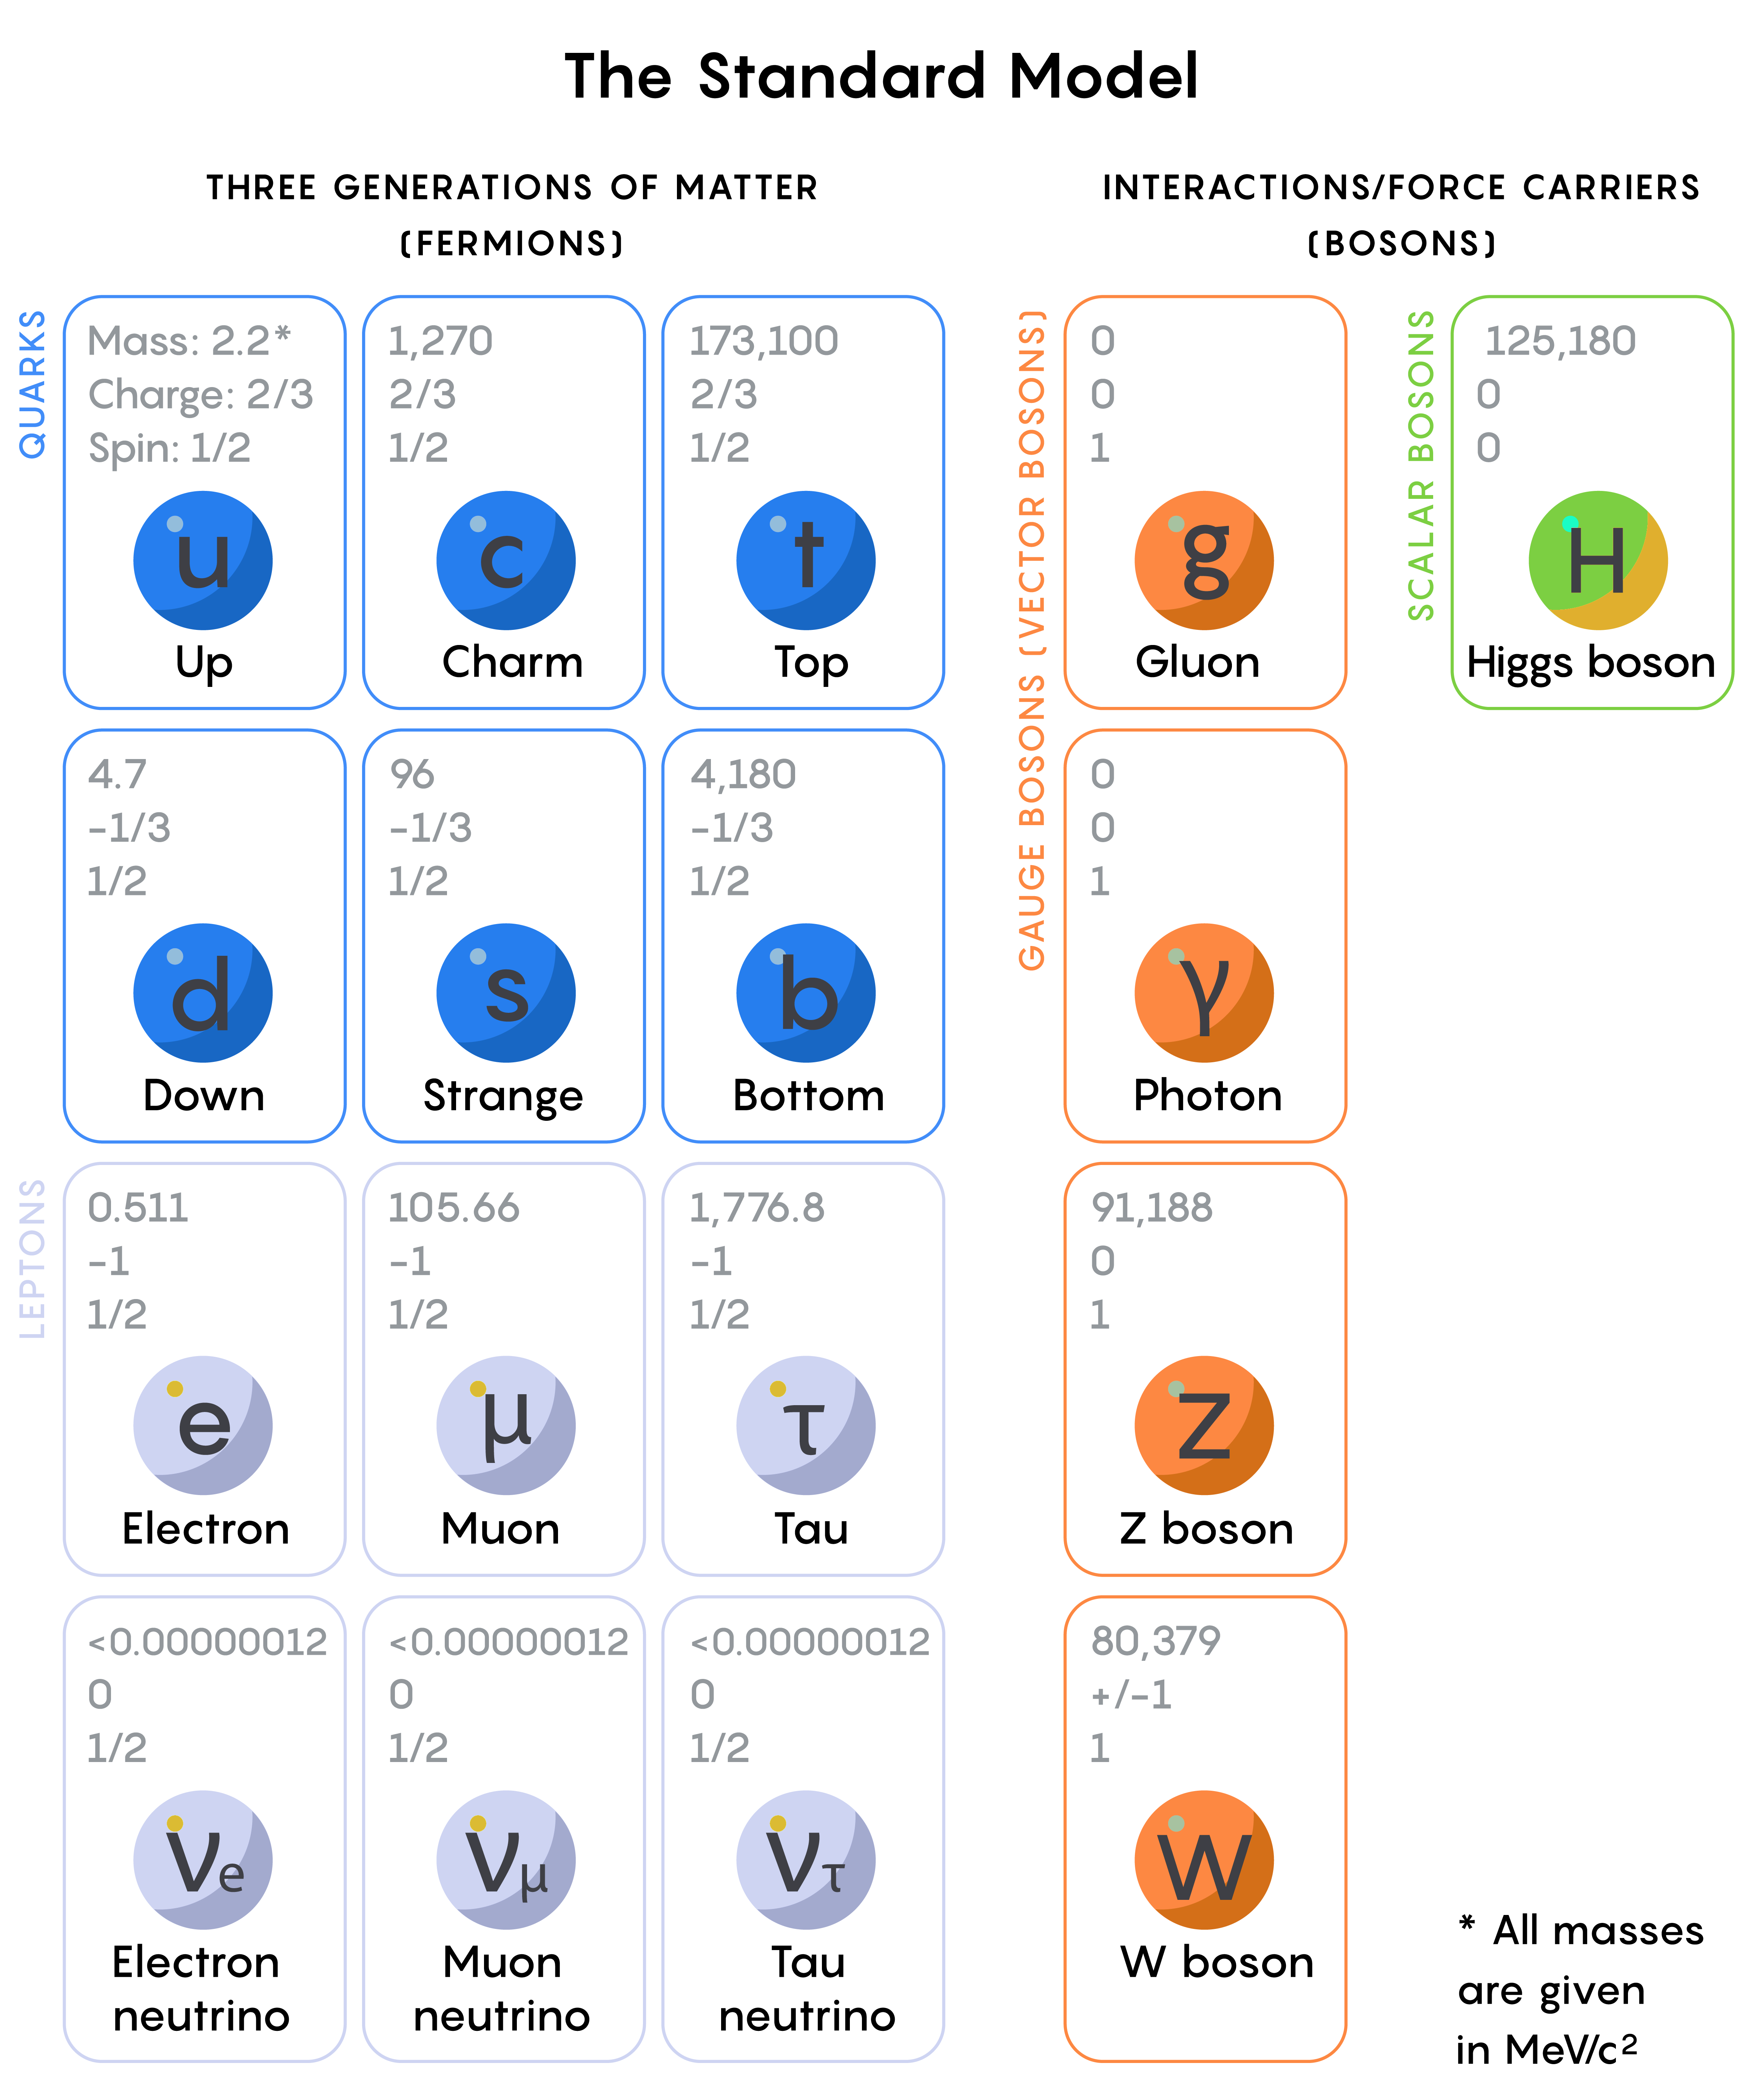
\includegraphics[width=1.0\textwidth]{Raster/SM_particles}
        \caption{
            The particles in the Standard Model of Particle Physics, with mass, charge, and spin. Taken from~\cite{quanta-magazine-2020}.
        }
        \label{fig:SM_particles}
    \end{figure}

    However, the Standard Model remains incomplete as it does not encompass gravity, 
    the fourth and weakest fundamental force, nor does it explain the observed 
    matter-antimatter asymmetry or the indirect evidence of dark matter. Therefore, 
    measuring Standard Model processes is crucial to uncovering discrepancies 
    between theory and experiment that could address these outstanding issues.

    In the following sections, we will discuss the symmetry principles,
    quantum field theory, the Standard Model of Particle Physics, and the gravitational extension.
    
    \subsection{Symmetry principles}
        The concept of symmetry is fundamental to the Standard Model. 
        According to the principle of Lorentz symmetry, the laws of 
        physics remain consistent for observers in different inertial reference 
        frames. This concept, along with quantum mechanics, bridges the gap between 
        classical mechanics and quantum field theories, which is essential for 
        understanding the Standard Model of particle physics.
        \subsubsection{Lagrangian formulation}
            In classical mechanics, the Lagrangian is a function of the
            generalised coordinates $q_i(t)$, generalised velocities $\dot{q}_i(t) = \frac{\text{d}q_i}{\text{d}t}$,
            and time $t$
            \begin{equation}
                L(q_i, \dot{q}_i) = T(q_i, \dot{q}_i) - V(q_i).
            \end{equation}
            where $T$ is the kinetic energy, and $V$ is the potential energy of the system.
            The action $S$ is defined as the integral of the 
            Lagrangian over time
            \begin{equation}
                S = \int L(q_i, \dot{q}_i) dt.
            \end{equation}
            The principle of least action states that the action $S$ is minimised
            along the path of motion of the system.
            A small perturbation, $q_i(t) \rightarrow q_i(t) + \delta q_i(t)$, should leave the action unchanged.
            The change in the action \( \delta S \) under the perturbation can be expressed as:
            \begin{equation}
                \delta S = 0 = \int_{t_1}^{t_2} \left( \delta q_i \frac{\partial L}{\partial q_i} + \delta \dot{q_i} \frac{\partial L}{\partial \dot{q_i}} \right) dt.
            \end{equation}
            This can be rearranged using integration by parts:
            \begin{equation}
                \delta S = 0 = \int_{t_1}^{t_2} \left( \delta q_i \frac{\partial L}{\partial q_i} + \frac{d}{dt} \left( \delta q_i \frac{\partial L}{\partial \dot{q_i}} \right) - \delta q_i \frac{d}{dt} \left( \frac{\partial L}{\partial \dot{q_i}} \right) \right) dt.
            \end{equation}
            By choosing the perturbation to vanish at the endpoints, the second term vanishes, and the equation simplifies to
            \begin{equation}
                \frac{\partial L}{\partial q_i} = \frac{d}{dt} \left( \frac{\partial L}{\partial \dot{q_i}} \right).
            \end{equation}
            This is the Euler-Lagrange equation, which describes the motion of the system.
        

            In field theories, the Lagrangian density, $L[\phi(x), \partial_{\mu}\phi(x)]$, is used instead of the $L$. 
            Here, $\phi(x)$ represents a scalar field dependent on the space-time four-vector $x$, 
            and $\partial_{\mu}\phi(x)$ is the derivative of the field with respect to the space-time coordinates
            \begin{equation}
                \partial_{\mu}\phi(x) = \frac{\partial \phi(x)}{\partial x^{\mu}}.
            \end{equation}
            The Lagrangian, as discussed in the previous paragraph, can be obtained by integrating the Lagrangian density over the space volume:
            \begin{equation}
                L = \int \mathcal{L}[\phi(x), \partial_{\mu}\phi(x)] d^{3}x.
            \end{equation}
            Additionally, the action S is defined by integrating the Lagrangian density over the entire four-dimensional spacetime:
            \begin{equation}
            S = \int \mathcal{L}[\phi(x), \partial_{\mu}\phi(x)] , d^{4}x.
            \end{equation}
            Similar to the classical mechanics, the Euler-Lagrange equation for the field $\phi(x)$ can be written as:
            \begin{equation}
                \partial_{\mu}(\frac{\partial \mathcal{L}}{\partial(\partial_\mu \phi)}) - \frac{\partial \mathcal{L}}{\partial \phi} = 0,
            \end{equation}
            following the same principle of least action. 
            Consider a free particle with mass $m$, the Lagrangian density can be written as:
            \begin{equation}
                \mathcal{L} = \frac{1}{2} \partial_{\mu}\phi(x) \partial^{\mu}\phi(x) - \frac{1}{2} m^{2} \phi^{2}(x).
            \end{equation}
            Using the Euler-Lagrange equation, the Klein-Gordon equation can be derived:
            \begin{equation}
                (\partial_{\mu}\partial^{\mu} + m^{2})\phi(x) = 0,
            \end{equation}
            which describes the motion of a free scalar field.
        \subsubsection{Symmetry and conservation Laws}
            Conservation laws are a direct consequence of the symmetry of the Lagrangian,
            not only in field theories but also in classical field theory and even in 
            the classical mechanics of point particles. For instance, symmetry under 
            time translation implies conservation of energy; symmetry under space 
            translation results in the conservation of momentum; and rotational 
            symmetry leads to the conservation of angular momentum. The Noether theorem
            states that for every symmetry of the Lagrangian
            there is a corresponding conserved quantity. Or, in field theory, for every
            symmetry of the Lagrangian density, there is a corresponding conserved current, 
            such that 
            \begin{equation}
                \partial_{\mu}j^{\mu} = 0.
            \end{equation}
            Consider a scalar field $\phi$, which undergoes an infinitesimal global transformation 
            $\phi \rightarrow \phi + \delta\phi$. Under such transformation, the Lagrangian density
            $\mathcal{L}[\phi, \partial_{\mu}\phi]$ remains invariant
            \begin{equation}
                \mathcal{L}[\phi, \partial_{\mu}\phi] \rightarrow \mathcal{L}[\phi, \partial_{\mu}\phi] + \delta\mathcal{L}(\phi, \partial_\mu\phi) = \mathcal{L}[\phi, \partial_{\mu}\phi],
            \end{equation}
            where $\delta\mathcal{L}(\phi, \partial_\mu\phi)$ is by definition zero. Expanding 
            $\delta\mathcal{L}(\phi, \partial_\mu\phi)$ in terms of $\phi$ and $\partial_\mu\phi$, 
            and using the Euler-Lagrange equation, the conserved current $j^{\mu}$ can be written as:
            \begin{equation}
                j^{\mu} = \frac{\partial \mathcal{L}}{\partial(\partial_{\mu}\phi)}\delta\phi,
            \end{equation}
            in this case, the conserved current is the Noether current.
        \subsubsection{Gauge symmetry}
            In the classical electromagnetic theory, the electric field $E$ and magnetic field $B$ are
            described by the Maxwell's equations,
            \begin{equation}
                \nabla \cdot \mathbf{E} = \frac{\rho}{\epsilon_0}, \\
                \nabla \cdot \mathbf{B} = 0,\\
                \nabla \times \mathbf{E} = -\frac{\partial \mathbf{B}}{\partial t},\\
                \nabla \times \mathbf{B} = \mu_0 \mathbf{J} + \mu_0 \epsilon_0 \frac{\partial \mathbf{E}}{\partial t},\\
            \end{equation}
            where $\rho$ is the charge density, $\mathbf{J}$ is the current density, 
            $\epsilon_0$ is the permittivity of free space, 
            and $\mu_0$ is the permeability of free space. 
            As implied by the Maxwell's equations, the magnetic fields
            are divergence-free, which implies that the magnetic field 
            can be described by a vector potential $\mathbf{A}$, such that
            $\mathbf{B} = \nabla \times \mathbf{A}$. The electric field
            can be described by a scalar potential $\phi$, such that
            $\mathbf{E} = -\nabla \phi - \frac{\partial \mathbf{A}}{\partial t}$.
            Both the scalar potential $\phi$ and the vector potential $\mathbf{A}$
            are not unique, as the electric and magnetic fields are invariant under
            the transformation $\phi \rightarrow \phi - \frac{\partial \Lambda}{\partial t}$,
            $\mathbf{A} \rightarrow \mathbf{A} + \nabla \Lambda$, where $\Lambda$ is an arbitrary
            function of space and time. This is known as the gauge symmetry of the electromagnetic field.

            The Maxwell's equations can be re-formulated by introducing the four-potential 
            $A^{\mu} = (\phi, \mathbf{A})$, such that the electromagnetic field tensor $F^{\mu\nu}$
            can be written as $F^{\mu\nu} = \partial^{\mu}A^{\nu} - \partial^{\nu}A^{\mu}$.
            The Maxwell's equations can be written in terms of the field tensor as:
            \begin{equation}
                \partial_{\mu}F^{\mu\nu} = \mu_0 J^{\nu},\hspace{0.2cm} 
                \partial_{\alpha} F_{\beta \gamma} + \partial_{\beta} F_{\gamma \alpha} + \partial_{\gamma} F_{\alpha \beta} = 0,\\
            \end{equation}
            where $J^{\nu} = (\rho, \mathbf{J})$ is the four-current. This is known as the covariant
            form of the Maxwell's equations. The gauge symmetry of the
            electromagnetic field can be written as $A^{\mu} \rightarrow A^{\mu} + \partial^{\mu}\Lambda$,
            where $\Lambda$ is an arbitrary function of space and time. 

            Using this formalism, the Lagrangian for an electromagnetic field can be expressed as follows:
            \begin{equation}
                \mathcal{L} = -\frac{1}{4}F^{\mu\nu}F_{\mu\nu} + A_{\mu}J^{\mu},
            \end{equation}
            The Lagrangian is invariant under gauge transformations, which is fundamental to the formulation 
            of quantum electrodynamics (QED). As we will show in the following chapter, the gauge symmetry 
            invariance leads to the interaction between the electromagnetic field and charged particles, for example, electrons 
            and positrons. This interaction is mediated by the exchange of photons, which are the gauge bosons
            of the electromagnetic field. 

    \subsection{Quantum electrodynamics}
        In the quest of finding an equation that would not only describe particles correctly
        and respect the symmetries of the Lorentz transformations, Paul Dirac proposed a first-order 
        linear differential equation, known as the Dirac equation,
        \begin{equation}
            (i\gamma^{\mu}\partial_{\mu} - m)\psi = 0,
        \end{equation}
        where $\psi$ is the Dirac spinor, $\gamma^{\mu}$ are the Dirac matrices, and $m$ is the mass of the particle.
        The $\gamma^{\mu}$ matrices are defined as follows:
        \begin{equation}
            \gamma^0 = \begin{pmatrix} I_2 & 0 \\ 0 & -I_2 \end{pmatrix},
            \gamma^i = \begin{pmatrix} 0 & \sigma^i \\ -\sigma^i & 0 \end{pmatrix},
        \end{equation}
        where $I_2$ is the identity matrix, and $\sigma^i$ are the Pauli matrices. 
        The Lagrangian of the Dirac field theory, which is based on the Dirac equation, can be written as:
        \begin{equation}
            \mathcal{L} = \bar{\psi}(i\gamma^{\mu}\partial_{\mu} - m)\psi,
        \end{equation}
        where $\bar{\psi} = \psi^{\dagger}\gamma^0$ is the Dirac adjoint. Using the Euler-Lagrange equation,
        the Dirac equation can be derived from the Lagrangian. 
        Under a global phase transformation $\psi \rightarrow e^{i\alpha}\psi$, the Lagrangian remains invariant,
        which implies that the Dirac field theory is invariant under global $U(1)$ transformations.
        However, the Dirac field theory is not invariant under local $U(1)$ transformations, where the phase
        transformation $\alpha$ is allowed to vary with space and time. To make the theory invariant under local
        $U(1)$ transformations, like in the classical field theory, a gauge field $A_{\mu}$ is introduced, 
        such that the covariant derivative $D_{\mu}$ can be written as:
        \begin{equation}
            D_{\mu} = \partial_{\mu} - iqA_{\mu},
        \end{equation}
        where $q$ is the charge of the particle. The full Lagrangian of the QED theory can be written as:
        \begin{equation}
            \mathcal{L}_{QED} = \bar{\psi}(i\gamma^{\mu}D_{\mu} - m)\psi - \frac{1}{4}F^{\mu\nu}F_{\mu\nu},
        \end{equation}
        Under a local $U(1)$ transformations, the first term of the Lagrangian remains invariant:
        \begin{equation}
            D_{\mu}\psi \rightarrow (\partial_{\mu} - iqA_{\mu})e^{iq\alpha}\psi = e^{iq\alpha}D_{\mu}\psi,
        \end{equation}
        The second term of the $\mathcal{L}_{QED}$, $F^{\mu\nu}F_{\mu\nu}$, which describes the the electromagnetic field, 
        is also invariant under local $U(1)$ transformations. 

        From a physics perspective, the QED theory describes the interaction between charged particles and the electromagnetic field.
        In the Dirac term in the Lagrangian, the covariant derivative \( D_\mu \) includes the electromagnetic interaction through the potential \( A_\mu \).
        And the interaction term \( ie \bar{\psi} \gamma^\mu A_\mu \psi \) shows how the charge particle field interacts with the electromagnetic field.
        The photon term in the Lagrangian, \( -\frac{1}{4} F^{\mu\nu} F_{\mu\nu} \), describes the quanta of electromagnetic field.
        The form of the QED Lagrangian also explains the massless nature of the photon, as including the photon mass term would break the gauge invariance of the theory.

        The QED theory is a renormalisable theory, to all orders in perturbation theory
        the divergences in the theory can be absorbed
        into the redefinition of the mass and charge of the particle. 

    \subsection{Quantum Chromodynamics}
        Quantum Chromodynamics (QCD) is the theory that describes the strong interaction, 
        which binds quarks and gluons into protons, neutrons, and other hadrons. 
        QCD is a type of quantum field theory known as a non-Abelian gauge theory, 
        based on the symmetry group SU(3). The Lagrangian of QCD is given by 
        the Yang-Mills equation:
        \begin{equation} \label{eq:QCD_Lagrangian}
            \mathcal{L}_{\text{QCD}} = \bar{\psi}(i\gamma^\mu D_\mu - m)\psi - \frac{1}{4}G_{\mu\nu}^a G^{a\mu\nu}.
        \end{equation}
        Here, $\psi$ represents the quark fields, $D_\mu = \partial_\mu - ig_s A_\mu^a T^a$
        is the covariant derivative, $A_\mu^a$ are the gluon fields, $T^a$ are the generators 
        of the SU(3) group, $g_s$ is the strong coupling constant, and 
        $G_{\mu\nu}^a = \partial_\mu A_\nu^a - \partial_\nu A_\mu^a + g_s f^{abc}A_\mu^b A_\nu^c$
        is the gluon field strength tensor, with \(f^{abc}\) being the structure constants of SU(3).

        To derive the QCD Lagrangian starting from the SU(3) transformation, we need to follow a few steps. 
        We will begin with the free Dirac Lagrangian and then introduce the SU(3) gauge fields. 
        The free Dirac Lagrangian that describes the motion of quarks is given by
        \begin{equation}
            \mathcal{L}_{\text{free}} = \bar{\psi}(i\gamma^\mu \partial_\mu - m)\psi,
        \end{equation}
        where $\psi$ is the quark field, $m$ is the quark mass, and $\gamma^\mu$
        are the gamma matrices.
        The quark field transforms under SU(3) as:
        \begin{equation}
            \psi \rightarrow U(x)\psi= e^{i\alpha^a(x)T^a}\psi,
        \end{equation}
        where $U(x)$ is an element of the SU(3) group, with $T^a$ being the generators of SU(3) 
        and $\alpha^a(x)$ being the parameters of the transformation.
        To maintain local SU(3) gauge invariance, we replace the partial derivative $\partial_\mu$
        with the covariant derivative $D_\mu$, defined as:
        \begin{equation}
            D_\mu = \partial_\mu - ig_s A_\mu^a T^a,
        \end{equation}
        where \(g_s\) is the strong coupling constant, \(A_\mu^a\) are the gluon fields.
        Similar to the QED, the covariant derivative now transforms as:
        \begin{equation}
            D_\mu\psi \rightarrow U(x)D_\mu\psi.
        \end{equation}
        Substitute the covariant derivative into the free Dirac Lagrangian
        \begin{equation}
            \mathcal{L}_{\text{QCD}} = \bar{\psi}(i\gamma^\mu D_\mu - m)\psi.
        \end{equation}
        This ensures that the Lagrangian is invariant under local SU(3) transformations.

        As we introduced, the kinetic term for the gluon fields is:
        \begin{equation}
            \mathcal{L}_{\text{gluon}} = -\frac{1}{4} G_{\mu\nu}^a G^{a\mu\nu}.
        \end{equation}
        Combining the quark and gluon parts, we obtain the full QCD Lagrangian in Equation \ref{eq:QCD_Lagrangian}

        In a non-Abelian group like SU(3), the generators \(T^a\) (where \(a = 1, 2, \ldots, 8\) 
        for SU(3)) do not commute. This means that for any two generators \(T^a\) and \(T^b\):
        \begin{equation}
            [T^a, T^b] = i f^{abc} T^c, \quad f^{abc} \neq 0.
        \end{equation}

        The form of the QCD Lagrangian is similar to the QED Lagrangian, with the quark 
        fields interacting with the gluon fields by term $g_s \bar{\psi} \gamma^\mu A_\mu^a T^a \psi$.
        The term $g_s f^{abc} A_\mu^b A_\nu^c$, shows that the gluons interact with each other, 
        unlike the photons in QED, giving rise to the self-interaction of the gluon fields.
        Physically, quarks come in three types of colour charges, conventionally labelled as red, 
        green, and blue. These colours are purely symbolic and represent the different states of 
        the SU(3) symmetry; anti-quarks carry anti-colours: anti-red, anti-green, and anti-blue.
        One of the most striking features of QCD is colour confinement, which means that quarks 
        and gluons are never found in isolation; they are always confined within hadrons. 
        The force between quarks does not diminish as they move apart. Instead, it remains 
        strong or even increases, preventing the isolation of individual quarks.
        At very short distances (high energies), the coupling constant $g_s$ becomes small, 
        and quarks behave as if they are free. 
        This phenomenon is known as asymptotic freedom, and it is one of the key features of QCD.
        To understand the running of $g_s$ we begin with the renormalisation group equation (RGE), 
        which governs the scale dependence of the coupling constant. The evolution of $g_s$ with 
        respect to the energy scale $\mu$ is described by the beta function, $\beta(g_s)$. At 
        one-loop level, the beta function for QCD is given by:
        \begin{equation}
            \beta(g_s) = \mu \frac{\partial g_s}{\partial \mu} = - \beta_0 \frac{g_s^3}{16\pi^2}.
        \end{equation}
        Here, $\beta_0$ is a constant that depends on the number of active quark flavours $n_f$. 
        Specifically, $\beta_0$ is expressed as
        \begin{equation}
            \beta_0 = 11 - \frac{2}{3} n_f
        \end{equation}
        For the case of QCD with three light quark flavours ($n_f = 3$), we have $\beta_0 = 9$.

        To determine how $g_s$ varies with the energy scale $\mu$, we integrate the renormalisation group equation
        \begin{equation}
            \frac{1}{g_s^2(\mu)} = \frac{1}{g_s^2(\mu_0)} + \frac{\beta_0}{8\pi^2} \ln \left( \frac{\mu}{\mu_0} \right).
        \end{equation}
        This equation illustrates how the strong coupling constant  $g_s$  evolves with the energy scale $\mu$. It 
        explicitly shows that $g_s$ decreases as $\mu$ increases, demonstrating the property of asymptotic freedom.
        It is often convenient to express the running of the coupling constant in terms of the strong coupling parameter \( \alpha_s \), defined as:
        \begin{equation}
            \alpha_s = \frac{g_s^2}{4\pi}
        \end{equation}
        Substituting $g_s$ in terms of $\alpha_s$ in the running equation, we obtain:
        \begin{equation}
            \alpha_s(\mu) = \frac{\alpha_s(\mu_0)}{1 + \frac{\alpha_s(\mu_0) \beta_0}{2\pi} \ln \left( \frac{\mu}{\mu_0} \right)}
        \end{equation}

        Figure~\ref{fig:QCD_running} shows the running of the strong coupling constant $\alpha_s$ with the energy scale $\mu$, as well 
        as experimental measurements of $\alpha_s$ at different energy scales from various experiments.
        \begin{figure}[htbp]
            \centering
            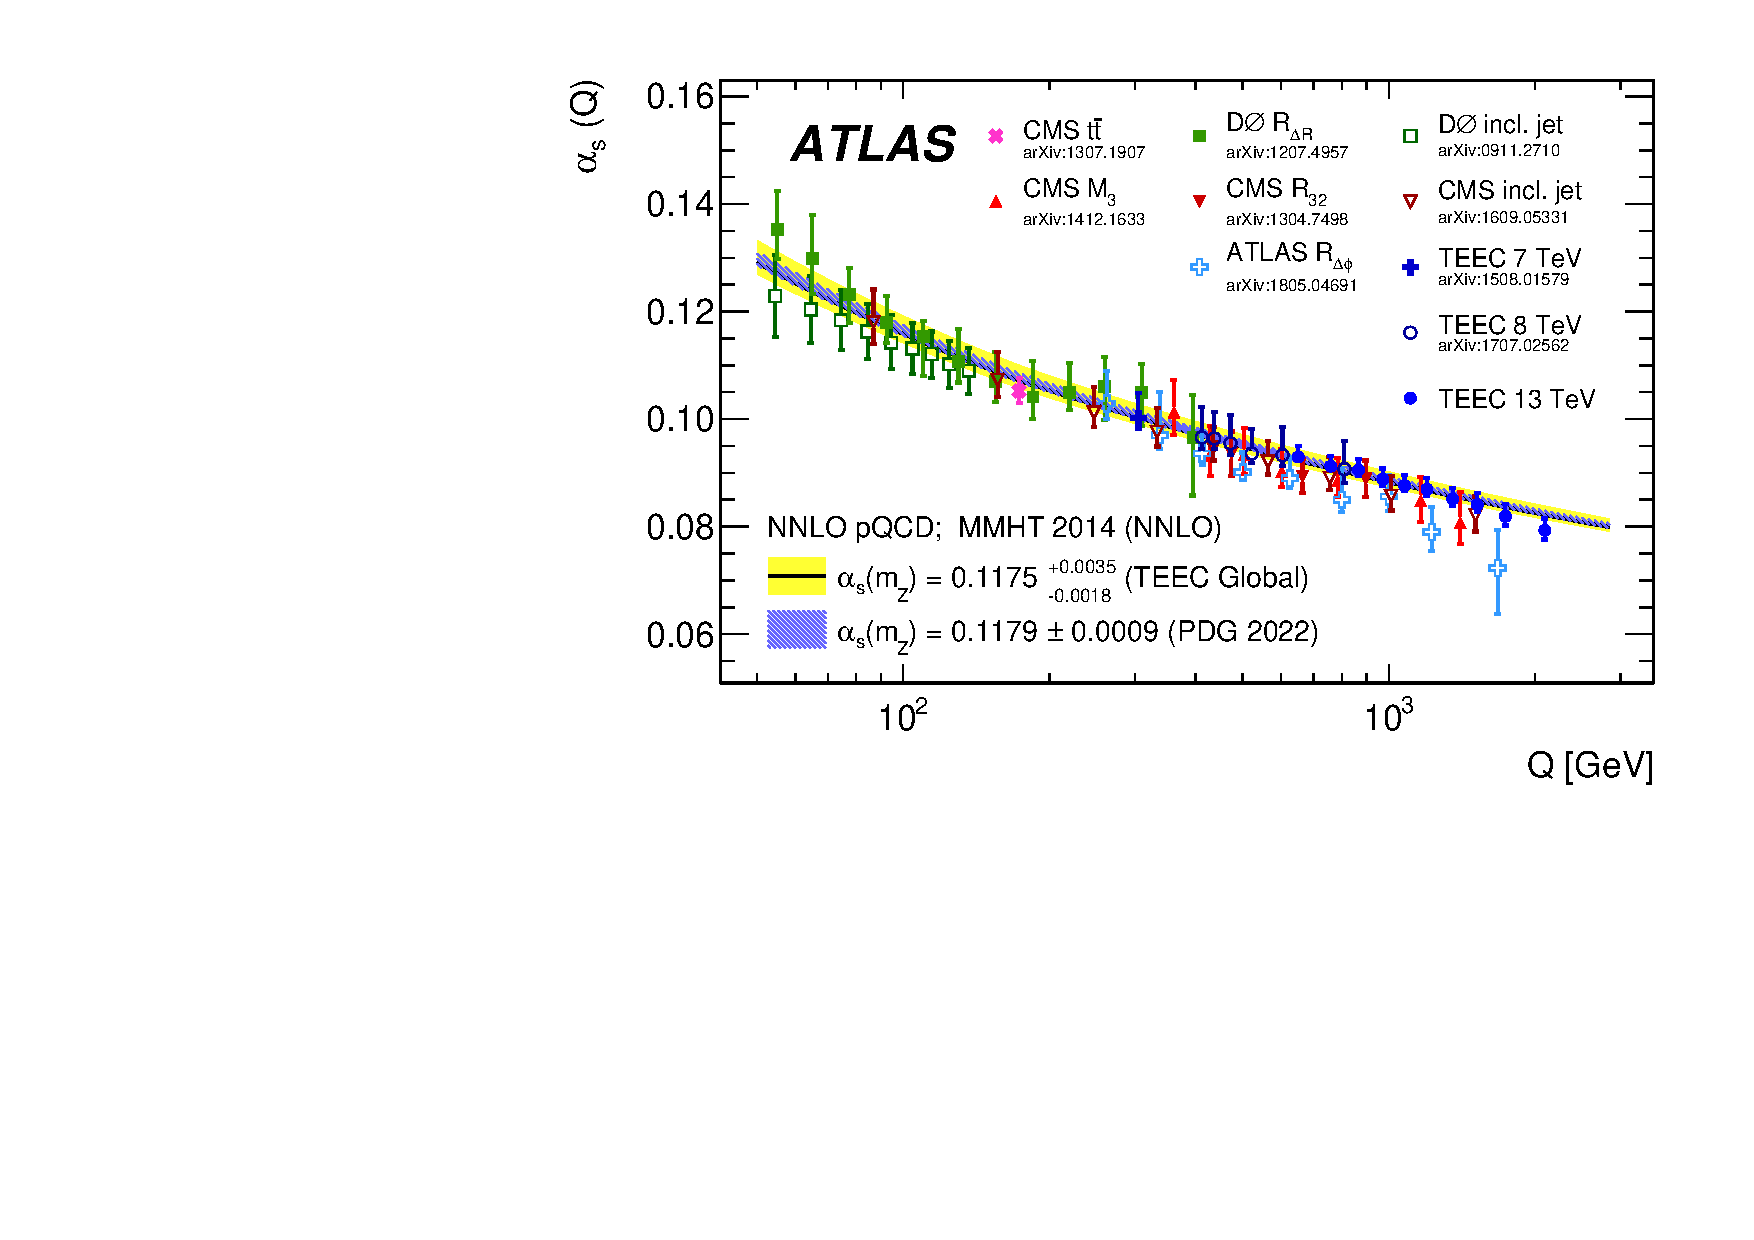
\includegraphics[width=0.6\textwidth]{Vector/QCD_running.pdf}
            \caption{
                The running of the strong coupling constant $\alpha_s$ with the energy scale $\mu$ in QCD, taken from~\cite{STDM-2018-51}.
                The coupling constant decreases as the energy scale increases, demonstrating asymptotic freedom.
                The experimental measurements of $\alpha_s$ at different energy scales are also shown.
            }
            \label{fig:QCD_running}
        \end{figure}

    \subsection{Weak force}
        The concept of the weak force emerged in the early 20th century with 
        the study of radioactive decay. In 1934, Enrico Fermi formulated a 
        theory of beta decay~\cite{Nanni_2019} that introduced the idea of a charged current weak interaction, 
        which was responsible for the transformation of a neutron into a proton,
        an electron, and an antineutrino. This interaction was initially thought 
        to be mediated by a contact force, similar to the classical idea of 
        collisions between billiard balls.
        The theoretical framework for understanding the weak force significantly 
        advanced in the 1950s and 1960s. The development of gauge theory and the 
        unification of electromagnetic and weak interactions into the electroweak 
        theory, proposed by Sheldon Glashow, Abdus Salam, and Steven Weinberg~\cite{PhysRev.127.965}, led 
        to a comprehensive understanding of the weak force. This theory was 
        experimentally confirmed by the discovery of the W and Z bosons in 1983~\cite{DiLella:2015yit} 
        at the CERN laboratory, for which the Nobel Prize was awarded.
        Despite its relatively short range and the fact that it is much weaker 
        than both the strong force and electromagnetism, the weak force is 
        responsible for a variety of processes that are fundamental to 
        particle physics and cosmology, such as beta decay, quark flavour change and
        CP violation.

        Chirality refers to the intrinsic property of fermions that distinguishes left-handed (L) 
        from right-handed (R) components. It is defined using the projection operators:
        \begin{equation}
            P_L = \frac{1}{2} (1 - \gamma_5), \quad P_R = \frac{1}{2} (1 + \gamma_5),
        \end{equation}
        where $ \gamma_5 = i\gamma^0\gamma^1\gamma^2\gamma^3 $ is the fifth gamma matrix in the Dirac algebra.
        Applying these projectors, the left-handed and right-handed components of a fermion field $\psi$ are:
        \begin{equation}
            \psi_L = P_L \psi = \frac{1}{2} (1 - \gamma_5) \psi, \quad \psi_R = P_R \psi = \frac{1}{2} (1 + \gamma_5) \psi.
        \end{equation}
        The charged weak interaction exclusively couples to left-handed fermions and right-handed antifermions. 
        This chiral nature of the weak force is a key feature distinguishing it from other fundamental forces.

        Isospin symmetry, originally introduced to describe the proton and neutron, can also be applied 
        to leptons within the context of the weak interaction.
        Leptons, like quarks, can be arranged into doublets under the $SU(2)_L$ symmetry of the weak interaction. 
        Each generation of leptons consists of a left-handed doublet and right-handed singlets. For the first generation:
        \begin{equation}
            \begin{pmatrix}
            \nu_e \\
            e
            \end{pmatrix}_L, \quad e_R
        \end{equation}
        Here, $\nu_e$ is the electron neutrino, and $e$ is the electron.
        The weak isospin ($I$) and its third component ($I_3$) are assigned as follows:
        \begin{itemize}
            \item The electron neutrino $\nu_e$ and electron $e$ form an isospin doublet with $I = \frac{1}{2}$.
            \item The third component of weak isospin $I_3$ for $\nu_e$ is $+\frac{1}{2}$, and for $e$ it is $-\frac{1}{2}$.
            \item Right-handed leptons, such as $e_R$, are singlets under $SU(2)_L$ and thus have $I = 0$.
        \end{itemize}

        The seminal experiment by Chien-Shiung Wu in 1957~\cite{PhysRev.105.1413} demonstrated parity violation in 
        the beta decay of cobalt-60. The electrons emitted in the decay exhibited a preferred 
        direction relative to the spin of the nuclei, indicating a violation of parity symmetry.
        The weak interaction Lagrangian, incorporating the \(SU(2)_L\) gauge fields, is given by:
        \begin{equation}
            \mathcal{L}_{\text{weak}} = \bar{\psi}_L i \gamma^\mu D_\mu \psi_L,
        \end{equation}
        where \(\psi_L\) represents the left-handed fermion doublets and \(D_\mu\) is the covariant derivative defined as:
        \begin{equation}
            D_\mu = \partial_\mu - i g \frac{\sigma^a}{2} W_\mu^a.
        \end{equation}
        Here, \(W_\mu^a\) are the gauge fields associated with \(SU(2)_L\), \(g\) is the coupling constant, and \(\sigma^a\) are the Pauli matrices.
        The presence of the $\gamma^5$ term results in the distinct treatment of left-handed and right-handed components, 
        leading to parity violation. The implications of this phenomenon includes 
        the observation that neutrinos are left-handed and antineutrinos are right-handed.

    \subsection{Electroweak unification and the Higgs mechanism}
        The electroweak theory in the Standard Model unifies the weak and electromagnetic interactions. 
        The Lagrangian includes terms for the gauge fields, their interactions with fermions, and the 
        Higgs mechanism. 
        \subsubsection{Electroweak unification}
            The gauge field terms describe the dynamics of the \(SU(2)_L\) and \(U(1)_Y\) gauge fields:
            \[
            \mathcal{L}_{\text{gauge}} = -\frac{1}{4} W_{\mu\nu}^a W^{a\mu\nu} - \frac{1}{4} B_{\mu\nu} B^{\mu\nu}.
            \]
            \( W_{\mu\nu}^a \) is the field strength tensor for the \(SU(2)_L\) gauge fields \( W_\mu^a \) (\(a = 1, 2, 3\)):
            \[
            W_{\mu\nu}^a = \partial_\mu W_\nu^a - \partial_\nu W_\mu^a + g \epsilon^{abc} W_\mu^b W_\nu^c,
            \]
            where \( g \) is the \(SU(2)_L\) coupling constant, and \(\epsilon^{abc}\) are the structure constants of \(SU(2)_L\).
            \( B_{\mu\nu} \) is the field strength tensor for the \(U(1)_Y\) gauge field \( B_\mu \):
            \[
            B_{\mu\nu} = \partial_\mu B_\nu - \partial_\nu B_\mu.
            \]
            The interaction of fermions with the gauge fields is described by the covariant derivative acting on the fermion fields:
            \[
            \mathcal{L}_{\text{fermion}} = \bar{\psi}_L i \gamma^\mu D_\mu \psi_L + \bar{\psi}_R i \gamma^\mu \partial_\mu \psi_R.
            \]
            \(\psi_L\) represents the left-handed fermion doublets:
            \[
            \psi_L = \begin{pmatrix} \nu_e \\ e \end{pmatrix}_L, \quad \begin{pmatrix} u \\ d' \end{pmatrix}_L,
            \]
            where \(d'\) is a linear combination of down-type quarks (\(d, s, b\)) due to quark mixing.
            \(\psi_R\) represents the right-handed fermion singlets:
            \[
            e_R, \quad u_R, \quad d_R.
            \]
            The covariant derivative \(D_\mu\) for left-handed fermions is:
            \[
            D_\mu = \partial_\mu - i g \frac{\tau^a}{2} W_\mu^a - i g' \frac{Y}{2} B_\mu,
            \]
            where \(\tau^a\) are the Pauli matrices, \(g\) and \(g'\) are the coupling constants for \(SU(2)_L\) and \(U(1)_Y\), respectively, and \(Y\) is the hypercharge.
        
            The Higgs mechanism involves the Higgs field \(\phi\), which breaks the electroweak symmetry and gives mass to the W and Z bosons:
            \[
            \mathcal{L}_{\text{Higgs}} = (D_\mu \phi)^\dagger (D_\mu \phi) - V(\phi).
            \]
            The covariant derivative \(D_\mu \phi\) is:
            \[
            D_\mu \phi = \left( \partial_\mu - i g \frac{\tau^a}{2} W_\mu^a - i g' \frac{Y}{2} B_\mu \right) \phi.
            \]
            The Higgs field \(\phi\) is an \(SU(2)_L\) doublet:
            \[
            \phi = \begin{pmatrix} \phi^+ \\ \phi^0 \end{pmatrix}.
            \]
            The Higgs potential \(V(\phi)\) is:
            \[
            V(\phi) = \mu^2 \phi^\dagger \phi + \lambda (\phi^\dagger \phi)^2.
            \]
        \subsubsection{Higgs mechanism and spontaneous symmetry breaking}
            The Higgs mechanism explains how the W and Z bosons acquire mass through spontaneous symmetry breaking of the electroweak symmetry.
            The Higgs field \(\phi\) acquires a non-zero vacuum expectation value (VEV):
            \[
            \langle \phi \rangle = \frac{1}{\sqrt{2}} \begin{pmatrix} 0 \\ v \end{pmatrix},
            \]
            where \(v \approx 246\) GeV is the VEV of the Higgs field.
            The potential \(V(\phi)\) has a minimum at \(\phi^\dagger \phi = \frac{v^2}{2}\), as shown in Figure~\ref{fig:higgs_potential}.
            \begin{figure}[hbtp]
                \centering
                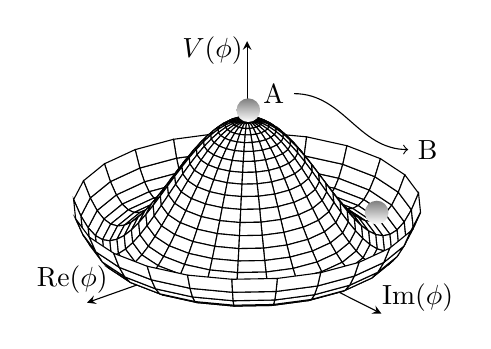
\begin{tikzpicture}
                    \begin{axis}[
                        axis lines=center,
                        view={140}{25},
                        axis equal,
                        domain=0:360,
                        y domain=0:1.25,
                        xmax=1.5,ymax=1.5,zmin=0,zmax=1.5,
                        x label style={at={(axis description cs:0.18,0.29)},anchor=north},
                        y label style={at={(axis description cs:0.82,0.25)},anchor=north},
                        z label style={at={(axis description cs:0.44,0.8)},anchor=north},
                        xlabel = $\mathrm{Re}(\phi)$,
                        ylabel=$\mathrm{Im}(\phi)$,
                        zlabel=$V(\phi)$,
                        ticks=none,
                        clip bounding box=upper bound
                        ]
                        \addplot3 [surf, shader=flat, draw=black, fill=white, z buffer=sort] ({sin(x)*y}, {cos(x)*y}, {(y^2-1)^2});
                    \end{axis}
                    \shade (3.47,3.5) circle [radius=0.15cm];
                    \shade (5.1,2.2) circle [radius=0.15cm];
                    \node[anchor=east] at (4.05,3.71) (text) {A};
                    \node[anchor=west] at (5.5,3.0) (description) {B};
                    \draw (description) edge[out=180,in=0,<-] (text);
                \end{tikzpicture}
                \caption{Higgs potential $V(\phi)$ with a minimum at $\phi^\dagger \phi = \frac{v^2}{2}$.}
                \label{fig:higgs_potential}
            \end{figure}
            When the Higgs field takes its VEV, the \(SU(2)_L \times U(1)_Y\) symmetry is spontaneously 
            broken down to \(U(1)_{\text{em}}\), the gauge symmetry of electromagnetism.
            Three of the four degrees of freedom in the Higgs doublet become the longitudinal 
            components of the W and Z bosons, giving them mass. 
            The remaining degree of freedom manifests as the physical Higgs boson.
        
            The masses of the W and Z bosons arise from the interaction between the gauge fields and the Higgs field.
            The charged W bosons (\(W^\pm\)) acquire mass through the term involving the Higgs VEV:
            \[
            (D_\mu \langle \phi \rangle)^\dagger (D_\mu \langle \phi \rangle).
            \]
            Expanding the covariant derivative:
            \[
            D_\mu \langle \phi \rangle = \left( \partial_\mu - i g \frac{\tau^a}{2} W_\mu^a - i g' \frac{Y}{2} B_\mu \right) \frac{1}{\sqrt{2}} \begin{pmatrix} 0 \\ v \end{pmatrix}.
            \]
            The term \(\frac{1}{2} g v W_\mu^1 - \frac{1}{2} g v W_\mu^2\) gives rise to the mass of the W bosons:
            \[
            M_W = \frac{gv}{2}.
            \]
            The neutral Z boson acquires mass similarly, but involves a mixture of \(W^3\) and \(B\):
            \[
            Z_\mu = \cos \theta_W W_\mu^3 - \sin \theta_W B_\mu,
            \]
            where \(\theta_W\) is the Weinberg angle. The mass of the Z boson is:
            \[
            M_Z = \frac{\sqrt{g^2 + g'^2} v}{2}.
            \]
            The photon remains massless because the corresponding combination of \(W^3\) and \(B\):
            \[
            A_\mu = \sin \theta_W W_\mu^3 + \cos \theta_W B_\mu,
            \]
            does not acquire a mass term from the Higgs mechanism.

        \subsubsection{Generation of fermion masses}
            The masses of the fermions (quarks and leptons) in the Standard Model 
            are generated through their interactions with the Higgs field. This 
            mechanism, known as the Yukawa interaction, couples the fermions to 
            the Higgs field, leading to mass terms once the Higgs field acquires 
            a VEV. 
            The Yukawa interactions describe the coupling between the Higgs field and
            the fermions. The relevant terms in the Lagrangian for a single generation 
            of quarks are:
            \[
            \mathcal{L}_{\text{Yukawa}} = -y_u \bar{Q}_L \tilde{\phi} u_R - y_d \bar{Q}_L \phi d_R + \text{h.c.}
            \]
            \(Q_L\) is the left-handed quark doublet:
            \[
            Q_L = \begin{pmatrix} u_L \\ d_L \end{pmatrix}.
            \]
            \(u_R\) and \(d_R\) are the right-handed up-type and down-type quark singlets, respectively.
            \(y_u\) and \(y_d\) are the Yukawa coupling constants for the up-type and down-type quarks, respectively.
            Recall the VEV of the Higgs field:
            \[
            \langle \phi \rangle = \frac{1}{\sqrt{2}} \begin{pmatrix} 0 \\ v \end{pmatrix}.
            \]
            Substituting the VEV of the Higgs field into the Yukawa Lagrangian, we obtain the mass terms for the quarks:
            \[
            \mathcal{L}_{\text{Yukawa}} = -y_u \bar{Q}_L \begin{pmatrix} 0 \\ \frac{v}{\sqrt{2}} \end{pmatrix} u_R - y_d \bar{Q}_L \begin{pmatrix} \frac{v}{\sqrt{2}} \\ 0 \end{pmatrix} d_R + \text{h.c.}
            \]
            This simplifies to:
            \[
            \mathcal{L}_{\text{Yukawa}} = -\frac{y_u v}{\sqrt{2}} \bar{u}_L u_R - \frac{y_d v}{\sqrt{2}} \bar{d}_L d_R + \text{h.c.}
            \]
            The terms \(\bar{u}_L u_R\) and \(\bar{d}_L d_R\) are Dirac mass terms for the up-type and down-type quarks, 
            respectively. Identifying the mass terms, we have:
            \[
            m_u = \frac{y_u v}{\sqrt{2}}, \quad m_d = \frac{y_d v}{\sqrt{2}}.
            \]
            Thus, the masses of the quarks are proportional to their respective Yukawa couplings.

            The generation of lepton masses follows a similar process, the Yukawa interactions for the leptons are given by:
            \[
            \mathcal{L}_{\text{Yukawa}} = -y_e \bar{L}_L \phi e_R + \text{h.c.}
            \]
            where \(L_L\) is the left-handed lepton doublet:
            \[
            L_L = \begin{pmatrix} \nu_{eL} \\ e_L \end{pmatrix}.
            \]
            where \(y_e\) is the Yukawa coupling constant for the electron.
            Substituting the VEV of the Higgs field into the Yukawa Lagrangian for leptons, we get:
            \[
            \mathcal{L}_{\text{Yukawa}} = -y_e \bar{L}_L \begin{pmatrix} 0 \\ \frac{v}{\sqrt{2}} \end{pmatrix} e_R + \text{h.c.}
            \]
            This simplifies to:
            \[
            \mathcal{L}_{\text{Yukawa}} = -\frac{y_e v}{\sqrt{2}} \bar{e}_L e_R + \text{h.c.}
            \]
            The term \(\bar{e}_L e_R\) is a Dirac mass term for the electron (or charged lepton), and the mass of the electron is:
            \[
            m_e = \frac{y_e v}{\sqrt{2}}.
            \]
            Therefore, the mass of the electron (or any charged lepton) is also proportional to its respective Yukawa coupling.
\section{A gravitational extension to the Standard Model}
        One potential extension for the SM to describe gravitation is proposed by Lisa Randall and Raman Sundrum~\cite{Graviton_theory},
        exploring the framework of a new higher-dimensional mechanism for solving the hierarchy problem~\cite{Arkani_Hamed_1998}.
        This model proposes a geometric solution to the hierarchy problem and predicts the existence of 
        Kaluza-Klein (KK) Graviton modes~\cite{Overduin_1997}. 
        Detailed explanations of technical aspects discussed briefly below can be found in ref.~\cite{Graviton_theory,Arkani_Hamed_1998,Overduin_1997}.
        The Randall-Sundrum (RS) model provides a geometric interpretation of the hierarchy 
        between the gravitational scale, \( M_P \sim 10^{18} \, \text{GeV} \), 
        and the weak scale, \( M_W \sim 10^2 \, \text{GeV} \). 
        In this model, the background geometry is a five-dimensional 
        Anti-de Sitter space (\( \text{AdS}_5 \)), characterised 
        by a constant negative curvature, and is truncated by two 
        four-dimensional Minkowski branes separated by a fixed distance~\cite{Arkani_Hamed_1998}.
        The model assumes that all relevant parameters arise naturally 
        from various powers of the five-dimensional fundamental scale, \( M_5 \sim M_P \).
        In the RS framework, the SM fields are confined to one of 
        the four-dimensional boundaries, commonly referred to as the 
        SM brane. The metric induced on this brane generates a 
        physical scale \( \Lambda_\pi \sim M_W \) from the 
        five-dimensional fundamental scale \( M_5 \), 
        achieved through an exponential geometric warp factor~\cite{Arkani_Hamed_1998}. 
        This warping effect eliminates the need to introduce 
        large hierarchies, as the exponential factor naturally 
        bridges the gap between the fundamental and electroweak scales.
        A key prediction of the RS model is the appearance of 
        spin-2 resonances, \( G^{(n)} \), which represent the 
        Kaluza-Klein (KK) excitations of the five-dimensional Graviton. 
        The masses and couplings of these resonances are determined 
        by the physical scale \( \Lambda_\pi \), making them potentially 
        significant for processes occurring at the weak scale.

        The RS model involves a 5D spacetime with the following metric:
        \[
        ds^2 = e^{-2kr_c|\phi|} \eta_{\mu\nu} dx^\mu dx^\nu - r_c^2 d\phi^2,
        \]
        where \( k \) is a scale of order the Planck scale. 
        \(\eta_{\mu\nu}\) is the 4D Minkowski metric. 
        \(\phi\) is the coordinate of the extra dimension, ranging from \(-\pi\) to \(\pi\).
        In this space, four-dimensional mass scales are related to five-dimensional mass parameters and the $e^{-2kr_c|\phi|}$, the warp factor.
        In the RS model, the Graviton field \(h_{\mu\nu}(x, \phi)\) can be expanded in terms of KK modes:
        \[
        h_{\mu\nu}(x, \phi) = \sum_{n=0}^{\infty} h_{\mu\nu}^{(n)}(x) \frac{e^{-2kr_c|\phi|}\chi^{(n)}(\phi)}{\sqrt{r_c}},
        \]
        where \(h_{\mu\nu}^{(n)}(x)\) are the 4D Graviton modes. 
        \(\chi^{(n)}(\phi)\) are the wave-functions of the KK modes that only depend on the extra dimension, \(\phi\) and \(r_c\).
        \(\chi^{(n)}(\phi)\) can be written as:
        \[
            \chi^{(n)}(\phi) \approx \frac{e^{2kr_c|\phi|}}{N_n}J_2\left(\frac{m_n}{k} e^{-kr_c|\phi|}\right),
        \]
        where $J_l$ is the $l^{th}$ order Bessel function. $m_n$ is the mass of the $n^{th}$ KK Graviton,
        and $N_n$ is a normalisation factor, given by:
        \[
            N_n \approx \frac{e^{kr_c\pi}}{\sqrt{kr_c}} J_2(x_n).
        \]
        The effective 4D Lagrangian for the interaction between KK Gravitons and the SM fields is:
        \[
        \mathcal{L}_{\text{eff}} = -[\frac{1}{M_P} h_{\mu\nu}^{(0)} T^{\mu\nu} - \frac{1}{\Lambda_\pi} \sum_{n=1}^{\infty} h_{\mu\nu}^{(n)}] T^{\mu\nu},
        \]
        where \(T^{\mu\nu}\) is the energy-momentum tensor of the SM fields and \(\Lambda_\pi = M_P e^{-kr_c\pi}\) is the effective scale on the TeV brane.
        Studies of the RS model have focused on the $\mathcal{L}_{\text{eff}}$ interaction. These interactions are only suppressed by $\Lambda_\pi$.
        In this thesis, we focus on the Graviton coupling to the SM Higgs boson, with low-TeV masses, the production cross section of the Higgs boson pairs 
        from the KK Graviton resonances is predicted to be significant at the current energy frontier.
        The 5D action, which describes gravity in the RS model, is:
        \[
        S_G = 2M_5^3 \int d^5x \sqrt{-G} R_5,
        \]
        where \(M_5\) is the 5D Planck scale, \(G\) is the determinant of the 5D metric \(G_{MN}\), and \(R_5\) is a 5D scalar.
        Interactions also occur between the \( G^{(n)} \) resonances arising from the \( S_G \). 
        The leading term in this self-coupling, in terms of powers of \( M_5^{-1} \), 
        is the triple Graviton vertex. 
        In four dimensions, this implies that the coupling between three 
        KK Gravitons \( \{ G^{(l)}, G^{(m)}, G^{(n)} \} \), 
        is governed by powers of \( \Lambda_\pi^{-1} \), 
        making it the dominant interaction within the KK Graviton sector.
    
\section{Modelling proton-proton collisions in particle physics}
    Proton-proton collisions, such as those studied at the Large Hadron Collider, 
    are complex processes modelled in several stages: parton distribution functions, hard scattering,
    parton showering, hadronisation, and underlying events. A typical collision
    is shown in Figure~\ref{fig:pp_collision}.

    \begin{figure}[htbp]
        \centering
        \includegraphics[width=1.0\textwidth]{Raster/pp-evt.pdf}
        \caption{
            Sketch of how a hadron collision is modelled. 
            In particular, one can notice the initial states, hard scattering, parton shower, hadronisation and the so-called underlying event. 
            From INFN web-page~\cite{pp_event_sketch}.
        }
        \label{fig:pp_collision}
    \end{figure}

    \subsection{Parton Distribution Functions (PDFs)}
        Protons are not fundamental particles; they are bound states of $uud$ quarks and gluons, collectively known as partons. 
        The PDF, \( f_i(x, Q^2) \), gives the probability density for finding a parton of type \( i \) (where \( i \) could 
        be \( u, d, s, c, t, b \) for quarks and \( g \) for gluons) with a momentum fraction \( x \) at a scale \( Q^2 \):
        \[
        f_i(x, Q^2) = x q_i(x, Q^2),
        \]
        where \( q_i(x, Q^2) \) is the number density of partons of type \( i \).
        The PDFs are extracted from experimental data and theoretical calculations 
        and are essential for predicting initial states in collisions.
        The Dokshitzer-Gribov-Lipatov-Altarelli-Parisi (DGLAP) equations describe how PDFs evolve with the energy scale \( Q^2 \):
        \[
        \frac{\partial f_i(x, Q^2)}{\partial \ln Q^2} = \sum_j \int_x^1 \frac{dy}{y} P_{ij}\left(\frac{x}{y}, \alpha_s(Q^2)\right) f_j(y, Q^2),
        \]
        where \( P_{ij}(z, \alpha_s) \) are the splitting functions, which describe the probability of a parton
        \( j \) splitting into a parton \( i \) with a fraction \( z \) of the momentum. And \( \alpha_s(Q^2) \) 
        is the strong coupling constant.

        The DGLAP equations can be written in a convolution form, showing the relationship between PDFs and splitting functions:
        \[
        \frac{\partial f_i(x, Q^2)}{\partial \ln Q^2} = \sum_j \left( P_{ij} \otimes f_j \right)(x, Q^2),
        \]
        where the convolution is defined as:
        \[
        \left( P_{ij} \otimes f_j \right)(x, Q^2) = \int_x^1 \frac{dy}{y} P_{ij}\left(\frac{x}{y}, \alpha_s(Q^2)\right) f_j(y, Q^2).
        \]
        In a proton-proton collision, the differential cross-section for a process \( pp \rightarrow X \) 
        involving partons \( i \) and \( j \) can be written as:
        \[
        d\sigma = \sum_{i,j} \int dx_1 dx_2 f_i(x_1, Q^2) f_j(x_2, Q^2) d\hat{\sigma}_{ij \rightarrow X},
        \]
        where \( d\hat{\sigma}_{ij \rightarrow X} \) is the partonic cross-section for the subprocess \( ij \rightarrow X \).
        One of the most widely used PDF sets are produced by the NNPDF (NN-based Parton Distribution Function) collaboration, 
        which uses neural networks to parameterise PDFs~\cite{Ball_2022}. 
        The NNPDF4.0NNLO sets are shown in Figure~\ref{fig:NNPDF40N2LO} for the PDFs at $Q = 3.2~\GeV$ and $Q = 100~\GeV$.
        This set approximates the PDFs at next-to-next-to-leading order (NNLO) precision.
        \begin{figure}[htbp]
            \centering
            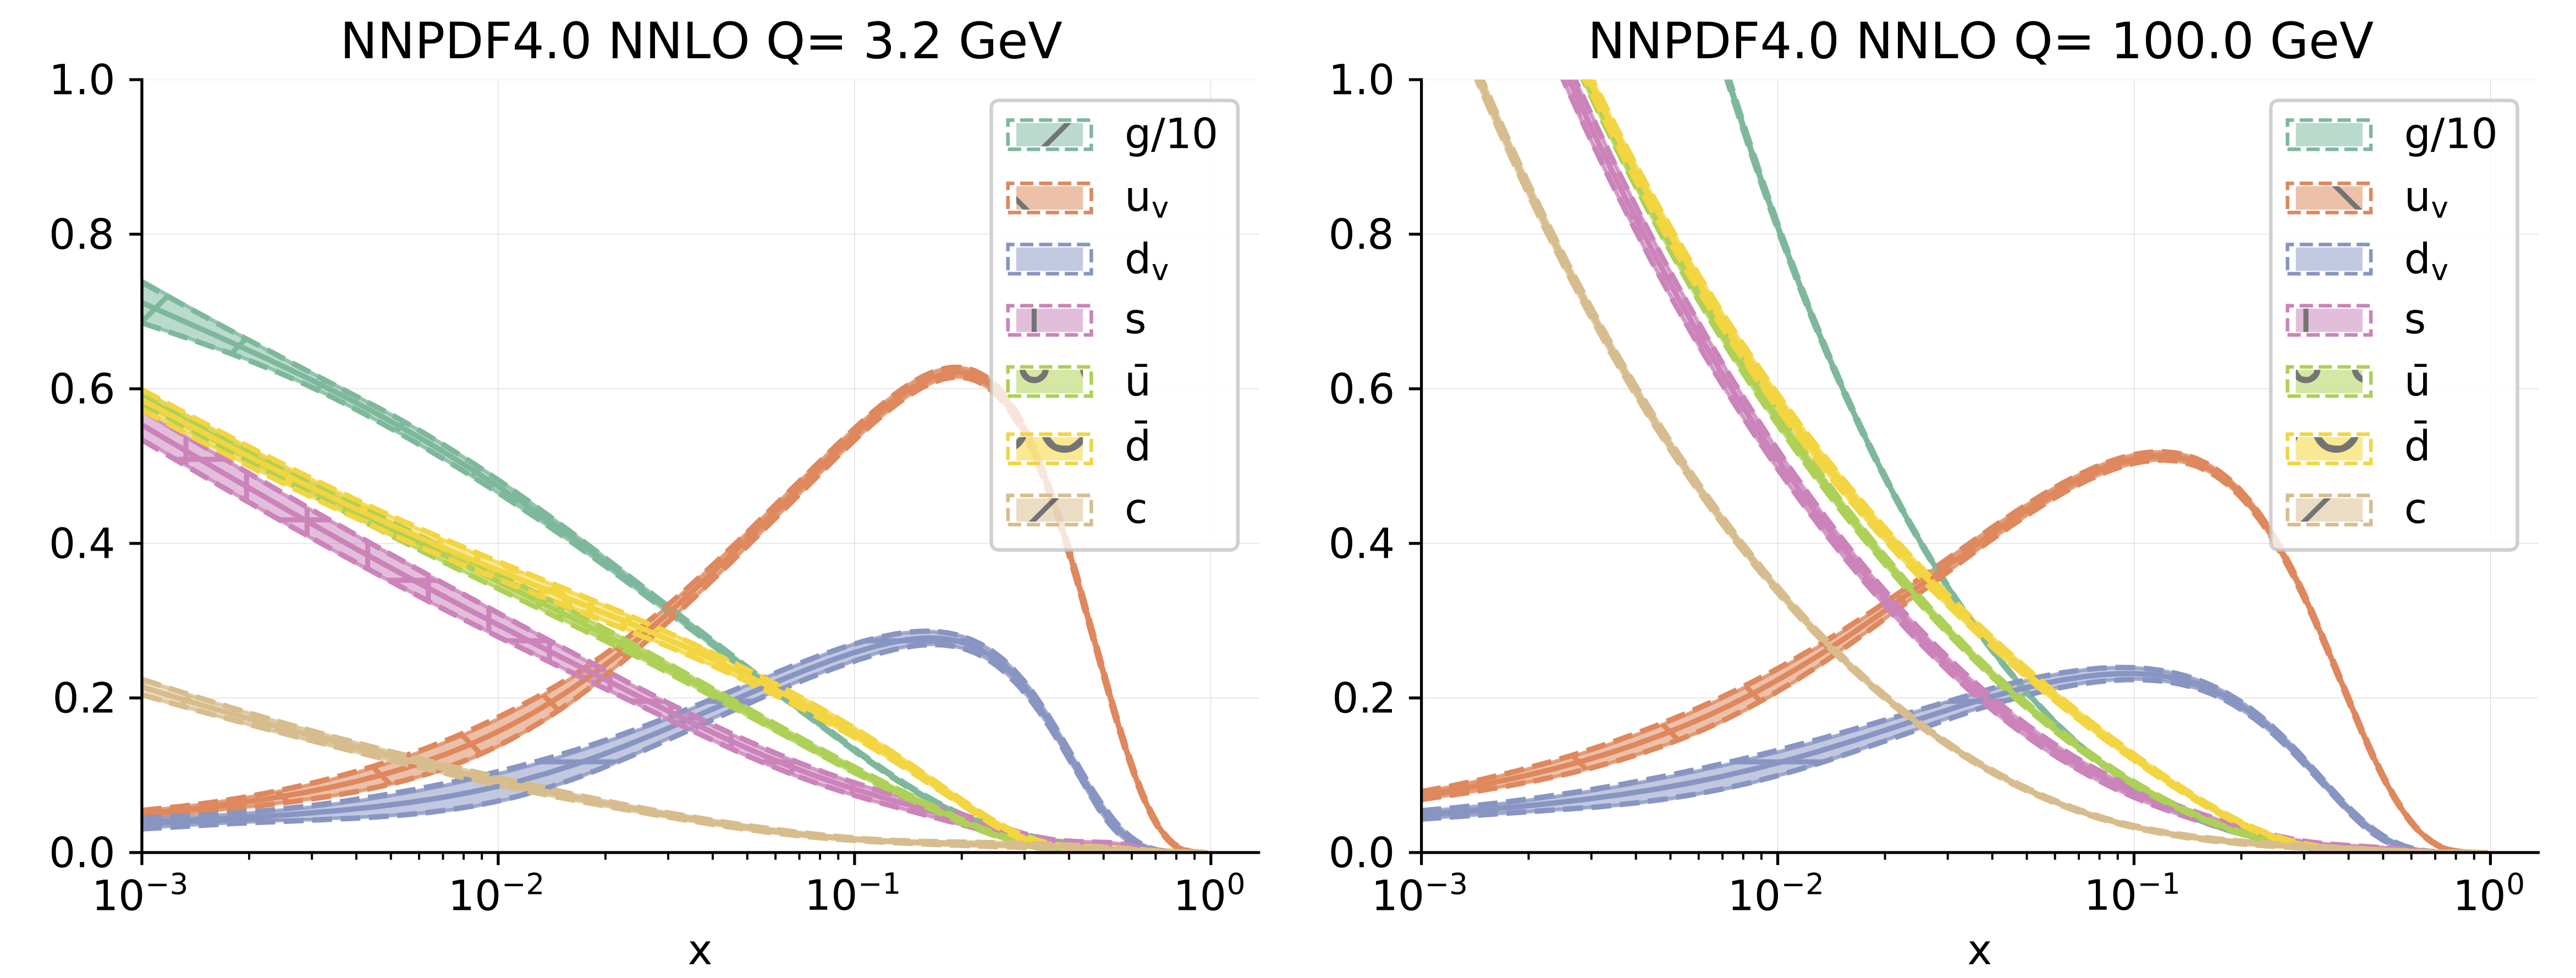
\includegraphics[width=1.0\textwidth]{Raster/nnpdf4.0.png}
            \caption{
                The NNPDF4.0NNLO parton distribution functions at $Q = 3.2~\GeV$ and $Q = 100~\GeV$~\cite{Ball_2022}.
            }
            \label{fig:NNPDF40N2LO}
        \end{figure}
        The latest NNPDF releases incorporate QED corrections, marking a significant step forward~\cite{thennpdfcollaboration2024photonsprotonimplicationslhc}. 
        They account for the photon parton distribution function, which, although a small correction, impacts the momentum fraction carried by the gluon. 
        The collaboration has made steps towards the next order of precision, approximate N3LO (Next-to-Next-to-Next-to-Leading Order). 
        The N3LO PDFs includes higher-order corrections in the PDFs, the predictions improves.
        The N3LO PDFs are consistent with NNLO results within uncertainties~\cite{thennpdfcollaboration2024pathn3lopartondistributions}.
        A significant milestone achieved by the NNPDF collaboration is the evidence for intrinsic charm quarks within the proton. 
        The intrinsic charm component was disentangled from charm-anticharm pairs arising from high-energy radiation, with a significance of three standard deviations~\cite{thennpdfcollaboration2022charmintrinsic}.

    \subsection{Parton shower, hadronisation, and underlying event}
        After the initial hard scatter, the high-energy partons undergo a cascade of emissions, producing more partons. 
        This process, described by perturbative QCD, includes both initial-state radiation (before the collision) and 
        final-state radiation (after the collision). The parton shower accounts for the sequential splitting of partons, 
        resulting in a multitude of lower-energy partons. 
        As partons cannot exist in isolation due to colour confinement, they must transform into colour-neutral hadrons. 
        hadronisation is a non-perturbative process where partons combine to form hadrons (e.g., pions, protons). 
        Two common models used to describe hadronisation are the Lund string model and cluster fragmentation. This 
        process occurs over a very short distance and time scale, effectively turning the showered partons into detectable 
        particles.
        Besides the primary hard scatter, other interactions occur in the collision, collectively known as the underlying event. 
        This includes additional soft parton interactions, beam-beam remnants (particles that do not participate in the hard scatter).
        The underlying event contributes to the overall activity observed in a collision 
        and must be accurately modelled to distinguish the signal from the background.
        Together, these processes transform the initial high-energy partons into a rich final state of hadrons that experimental 
        detectors can observe and analyse. Understanding each stage is crucial for accurate simulation and interpretation of collider data.
    %!TEX root = ../thesis.tex
%*******************************************************************************
%****************************** Third Chapter **********************************
%*******************************************************************************
\chapter{The ATLAS detector at the LHC}

% **************************** Define Graphics Path **************************

\graphicspath{{1_MainChapters/Chap3_ATLAS/Figs}}

\section{CERN and the Large Hadron Collider (LHC)}
    The European Organisation for Nuclear Research, known as CERN, was founded in 1954 with the aim of establishing 
    a world-class laboratory for particle physics research. Located on the border between France and Switzerland, 
    near Geneva, CERN was established by 12 European countries to promote scientific collaboration in post-war Europe. 
    Its creation marked a significant step in fostering international cooperation in the field of fundamental physics.
    The modern CERN accelerator complex is shown in Figure~\ref{fig:LHC}.
    \begin{figure}[t]
        \centering
        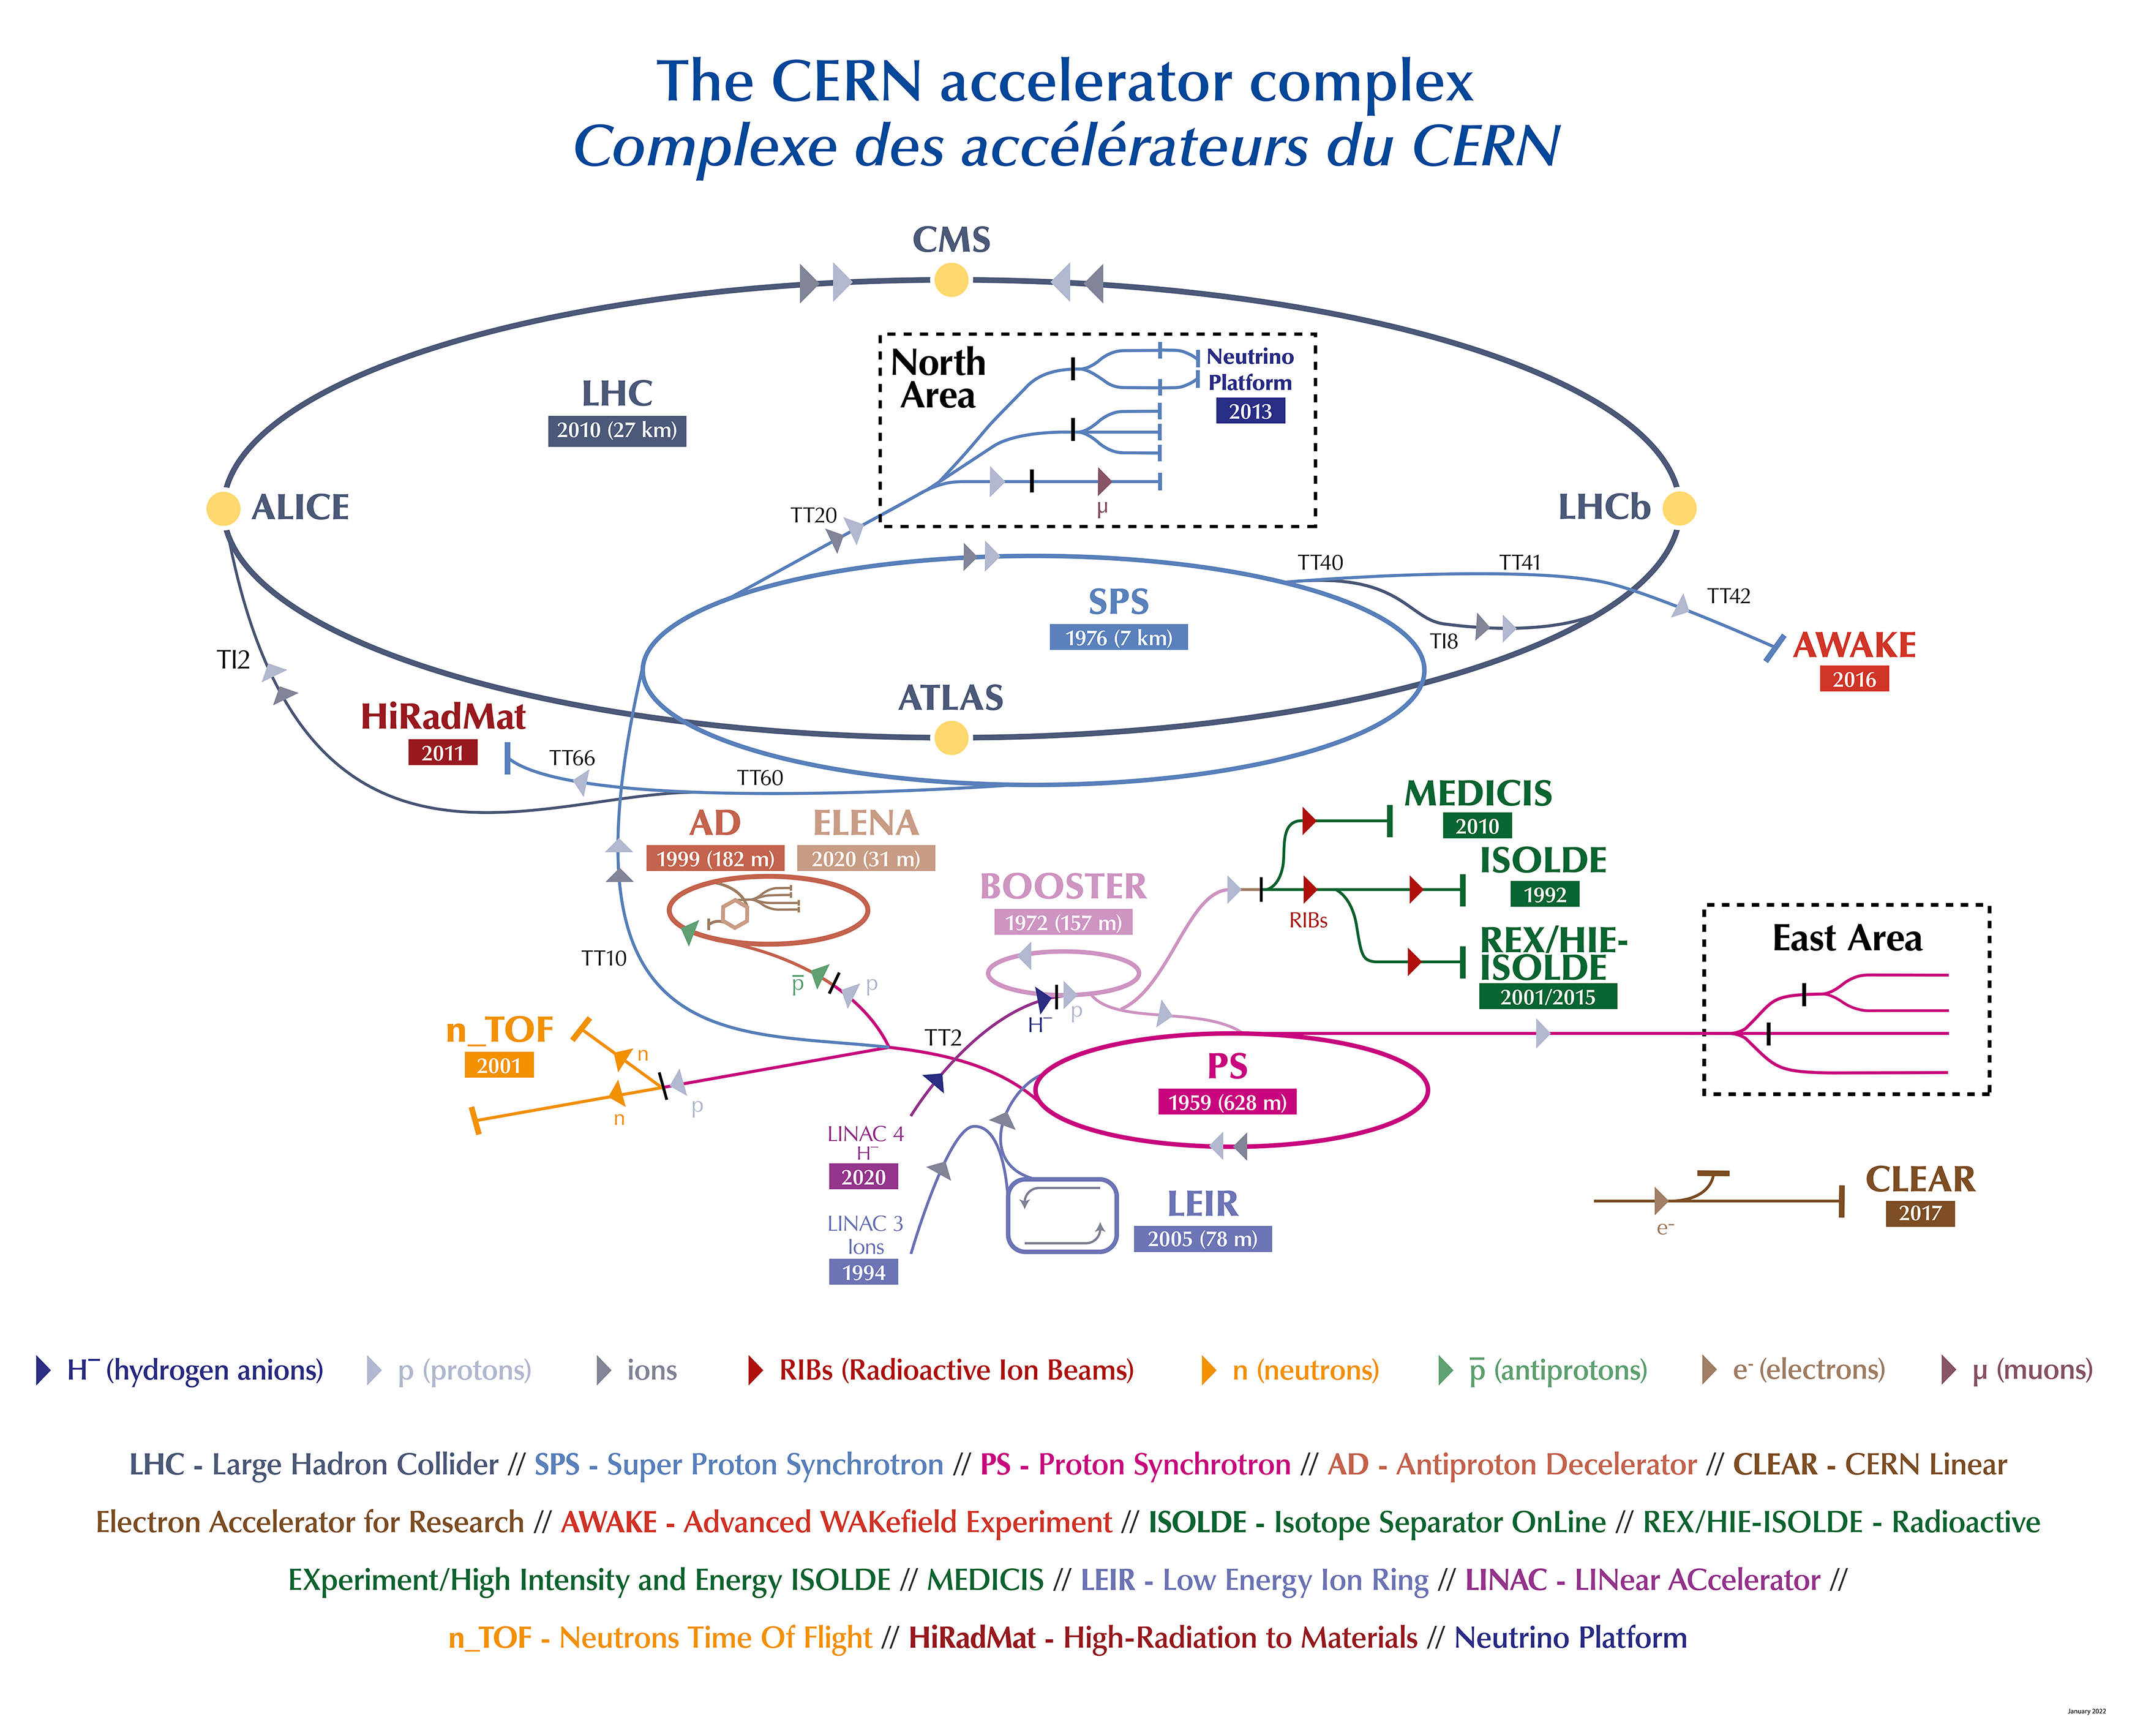
\includegraphics[width=1.0\textwidth]{CCC-v2022-small.png}
        \caption{The CERN accelerator complex, including the Large Hadron Collider (LHC) and its experiments, taken from~\cite{CERNAccComp}}
        \label{fig:LHC}
    \end{figure}

    CERN's early years were marked by the construction of pioneering accelerators, such as the Synchrocyclotron (SC)~\cite{Synchro-CyclotronDivision:1606751}
    in 1957 and the Proton Synchrotron (PS) in 1959~\cite{ADAMS1960}. The SC was CERN's first accelerator, used for nuclear physics 
    experiments, while the PS, with a beam energy of 28 GeV, became instrumental in numerous discoveries, including 
    the observation of neutral currents in 1973. The PS's success laid the groundwork for more advanced facilities 
    and experiments.

    In 1976, the Super Proton Synchrotron (SPS)~\cite{Doble:2312568} began operations, serving both as a particle accelerator and a storage 
    ring. The SPS played a pivotal role in the discovery of the W and Z bosons in 1983, work that earned Carlo Rubbia 
    and Simon van der Meer the Nobel Prize in Physics. These discoveries helped confirm the electroweak theory, a fundamental 
    component of the Standard Model of particle physics.

    The Large Electron-Positron Collider (LEP)~\cite{Schopper:2009zz} was a groundbreaking particle accelerator that operated at CERN from 1989 to 2000. 
    Situated in the same 27-kilometre tunnel that now houses the LHC, LEP was designed to collide electrons and positrons at high 
    energies to probe the fundamental constituents of matter. The construction of LEP was a significant engineering and scientific 
    achievement, involving the development of advanced technologies and large-scale international collaboration. One of the 
    notable accomplishments of LEP was its precision measurements of the Z boson~\cite{ALEPH:2007brf}, which helped to confirm the electroweak theory. 
    The collider's ability to produce clean and precise collisions of electrons and positrons allowed physicists to explore a wide 
    range of phenomena with unprecedented accuracy. Over its 11 years of operation, LEP produced a wealth of scientific results 
    that significantly enhanced our understanding of particle physics and laid the groundwork for future discoveries.

    When LEP was decommissioned in 2000, its tunnel was repurposed for the LHC, which required substantial upgrades to 
    handle the higher energy collisions of protons and heavy ions. 
    The LHC~\cite{Evans:2008zzb}, the most ambitious project at CERN, was officially inaugurated on October 21, 2008. 
    It is designed to collide protons at unprecedented centre-of-mass energy levels, reaching up to 13.6 TeV. The LHC's primary 
    objective is to explore the fundamental properties of matter and the forces governing the universe that beyond the Standard Model.
    The LHC hosts several major experiments, each with specific research goals and sophisticated detection apparatus.
    ATLAS (A Toroidal LHC ApparatuS)~\cite{PERF-2007-01} and CMS (Compact Muon Solenoid)~\cite{CMS-CMS-00-001} are general-purpose detectors. These experiments 
    played a central role in the discovery of the Higgs boson in 2012, a particle essential to the Standard Model as 
    it provides evidence for the mechanism by which other elementary particles acquire mass. 
    The LHCb (Large Hadron Collider beauty)~\cite{LHCb:2008vvz} experiment focuses on investigating the differences between matter and antimatter by studying the decays 
    of particles containing b (beauty) quarks. This research aims to understand why the universe is dominated by 
    matter rather than antimatter, despite the expectation that both should have been produced in equal amounts 
    during the Big Bang.
    ALICE (A Large Ion Collider Experiment)~\cite{ALICE:2008ngc} is designed to study the properties of quark-gluon plasma, a state of matter thought to have existed shortly 
    after the Big Bang. By colliding heavy ions, ALICE aims to recreate and analyse this plasma, providing insights 
    into the strong force that binds quarks and gluons together to form protons and neutrons.
    TOTEM (TOTal Elastic and diffractive cross-section Measurement)~\cite{totem_2008} and LHCf (Large Hadron Collider forward) focus on studying forward particles, 
    those that travel close to the beamline, to gain insights into proton structure and the underlying dynamics of particle collisions. 
    TOTEM measures the total cross-section, elastic scattering, and diffraction processes, while LHCf studies particles produced at very small 
    angles to the beam direction.

    \subsection{The operation of the LHC}
        The LHC's operational phases have significantly advanced particle physics, combining upgrades and high-energy 
        collisions to explore the fundamental aspects of matter and the universe. The ongoing and future upgrades, especially 
        the HL-LHC, promise to further enhance our understanding and potentially lead to groundbreaking discoveries. 
        \subsubsection{Run 1 (2009-2013)}
            Run 1 of the Large Hadron Collider (LHC) at CERN began in 2009 and continued until early 2013. 
            During this period, the LHC operated at proton-proton (p-p) collision energies of 7~TeV (2010-2011) and 8~TeV (2012-2013), 
            laying the groundwork for significant scientific discoveries and establishing the LHC as 
            the world's most powerful particle accelerator. The most notable achievement of Run 1 was the 
            discovery of the Higgs boson~\cite{HIGG-2012-27,CMS-HIG-12-028} in July 2012 by the ATLAS and CMS experiments. This discovery confirmed 
            the last missing component of the Standard Model of particle physics and garnered the 2013 Nobel 
            Prize in Physics for theorists Francois Englert and Peter Higgs. Run 1 also involved extensive searches 
            for new physics beyond the Standard Model, including searches for supersymmetry (SUSY) and extra 
            dimensions, although no definitive evidence was found.
            Lead-lead (Pb-Pb) and proton-lead (p-Pb) collisions were also conducted during Run 1. 
            Run 1 marked the successful commissioning of the LHC's complex systems, including its superconducting magnets, cryogenics, and detectors.
            Significant advancements in data acquisition and analysis techniques were developed, setting the stage for future runs.
        \subsubsection{Long Shutdown 1 (2013-2015)}
            Following the successful completion of Run 1, the LHC entered Long Shutdown 1 (LS1) from early 2013 to early 2015. During this period, 
            significant maintenance and upgrades were carried out to prepare the LHC for higher energy collisions and increased luminosity in 
            subsequent runs. LS1 involved enhancements to the accelerator's magnets, cryogenics, and beam instrumentation, ensuring improved 
            performance and reliability.
        \subsubsection{Run 2 (2015-2018)}
            The LHC resumed operations in 2015 with Run 2. 
            This phase saw the LHC operate at the higher energy of 13 TeV, leading to further significant discoveries 
            and more precise measurements of the Higgs boson and other Standard Model particles~\cite{ParticleDataGroup:2022pth}. 
            The increased energy 
            and luminosity provided new opportunities to search for physics beyond the Standard Model, although no 
            new particles were discovered.
        \subsubsection{Long Shutdown 2 (2019-2021)}
            Following Run 2, the LHC entered Long Shutdown 2 (LS2) for maintenance and upgrades to prepare for even higher 
            luminosity operations. The upgrades aimed to enhance the performance of the accelerator and detectors~\cite{Arduini_2024}, ensuring 
            improved data quality and higher collision rates.
            The COVID-19 pandemic had a notable impact on CERN's LS2. The pandemic necessitated strict health and safety 
            measures, significantly affecting on-site work. CERN implemented remote working protocols and minimised on-site 
            activities to protect staff and contractors. These disruptions caused delays in the planned maintenance and 
            upgrades to the LHC and associated experiments. Despite these challenges, CERN managed to continue essential 
            work, ensuring that critical upgrades were completed, albeit on a postponed schedule. 
        \subsubsection{Run 3 (2022-present)}
            Run 3 began in 2022, operating at 13.6 TeV with further optimised conditions. This phase focuses on collecting 
            more data to enhance the precision of existing measurements and explore new potential discoveries. 
            Operating at higher energy required extensive calibration and tuning of the accelerator 
            components to handle the increased energy and collision rates effectively. Global supply chain issues delayed the delivery of critical components, hindering 
            technical improvements and maintenance work essential for efficient LHC operation during LS2~\cite{Perrot:2845779,covid19_economics}.
            Extensive calibration and validation of upgraded detectors were necessary to ensure accurate and reliable measurements, initially slowing down data collection.
            Despite these challenges, the LHC has ramped up its performance as technical issues are resolved in 2024. The 
            upgraded systems are fully integrated and optimised. In run 3 the LHC has delivered over 160~\ifb of data to the ATLAS and CMS 
            experiments at the time of writing, with 101~\ifb collected in 2024 alone. 

    \subsection{Future LHC upgrades - The High-Luminosity LHC}
        The High-Luminosity Large Hadron Collider (HL-LHC)~\cite{HighLuminosityLHC} is a major upgrade to the current LHC, designed to increase 
        its luminosity by a factor of 5-10. Scheduled to start operations in the late-2020s, the HL-LHC aims to gather 
        approximately 10 times more data than the existing LHC. This significant increase in luminosity will enhance 
        the potential for new discoveries and provide more precise measurements of SM phenomena. 

        The HL-LHC will feature new, stronger superconducting magnets to better focus the proton beams, increasing the luminosity.
        Upgraded cryogenic systems will enhance the cooling power of the accelerator, crucial for maintaining the superconducting state of the magnets.
        The ATLAS, CMS, LHCb, and ALICE detectors will undergo significant enhancements to handle the increased collision 
        rates and data throughput, ensuring they can capture and process the additional information effectively.
        Components will be upgraded to withstand the higher levels of radiation expected from the increased luminosity, 
        ensuring the longevity and reliability of the detector systems.
    
    \subsection{Future collider projects - the Future Circular Collider (FCC)}
        FCC~\cite{Benedikt2020} represents 
        a bold vision for the next generation of particle accelerators, aiming to 
        build upon the discoveries of the HL-LHC. The FCC is a proposed research 
        infrastructure that would significantly extend our understanding of 
        fundamental physics by exploring uncharted energy scales and precision 
        measurements. It is designed to address key questions that remain unanswered 
        in the Standard Model of particle physics and beyond.
        The FCC project encompasses two main collider configurations: the FCC-ee, 
        a high-luminosity electron-positron collider, and the FCC-hh, a high-energy 
        proton-proton collider. The FCC-ee is envisaged as a first step, providing 
        precise measurements of the Higgs boson, W and Z bosons, and the top quark, 
        while the FCC-hh will follow, offering collisions at energies up to 100 TeV, 
        far exceeding the capabilities of the LHC.
        \subsubsection{The FCC-ee: A Precision Machine}
        The FCC-ee collider is designed to operate at various energy stages, initially 
        focusing on Z boson production with centre-of-mass energies around 90 GeV, 
        and subsequently increasing to study the W boson, Higgs boson, and top quark 
        at higher energies. With its unprecedented luminosity and precision, the FCC-ee 
        will provide high-precision measurements of the Higgs boson properties, 
        improved determinations of the W and Z boson masses and couplings, and detailed studies of
        the top quark. The FCC-ee's exceptional precision will allow physicists to probe 
        for tiny deviations from the SM predictions, potentially revealing 
        new physics.
        \subsubsection{The FCC-hh: Exploring the Energy Frontier}
        Following the FCC-ee, the FCC-hh collider aims to push the energy frontier to 
        100 TeV, offering unprecedented opportunities for discovery. The key objectives 
        of the FCC-hh include probing the nature of dark matter by potentially producing 
        dark matter particles through their interactions with SM particles; 
        exploring the Higgs potential and self-interactions to understand the stability 
        of the Higgs field; searching for new particles and forces that could manifest 
        at higher energy scales, providing insights into physics beyond the SM.
        To achieve these goals, the FCC-hh will require significant advancements in 
        technology, including the development of stronger superconducting magnets 
        capable of reaching magnetic fields up to 16~T, and sophisticated detectors 
        designed to handle the higher energy and luminosity.

\section{The ATLAS detector}
    The ATLAS detector~\cite{PERF-2007-01}, installed at Point 1 of the LHC at CERN, 
    is one of the largest and most complex particle detectors ever constructed. A cut-away 
    view of the ATLAS detector in Run 3 configuration is shown in Figure~\ref{fig:ATLAS_cutaway_run3}.
    \begin{figure}[htbp]
        \centering
        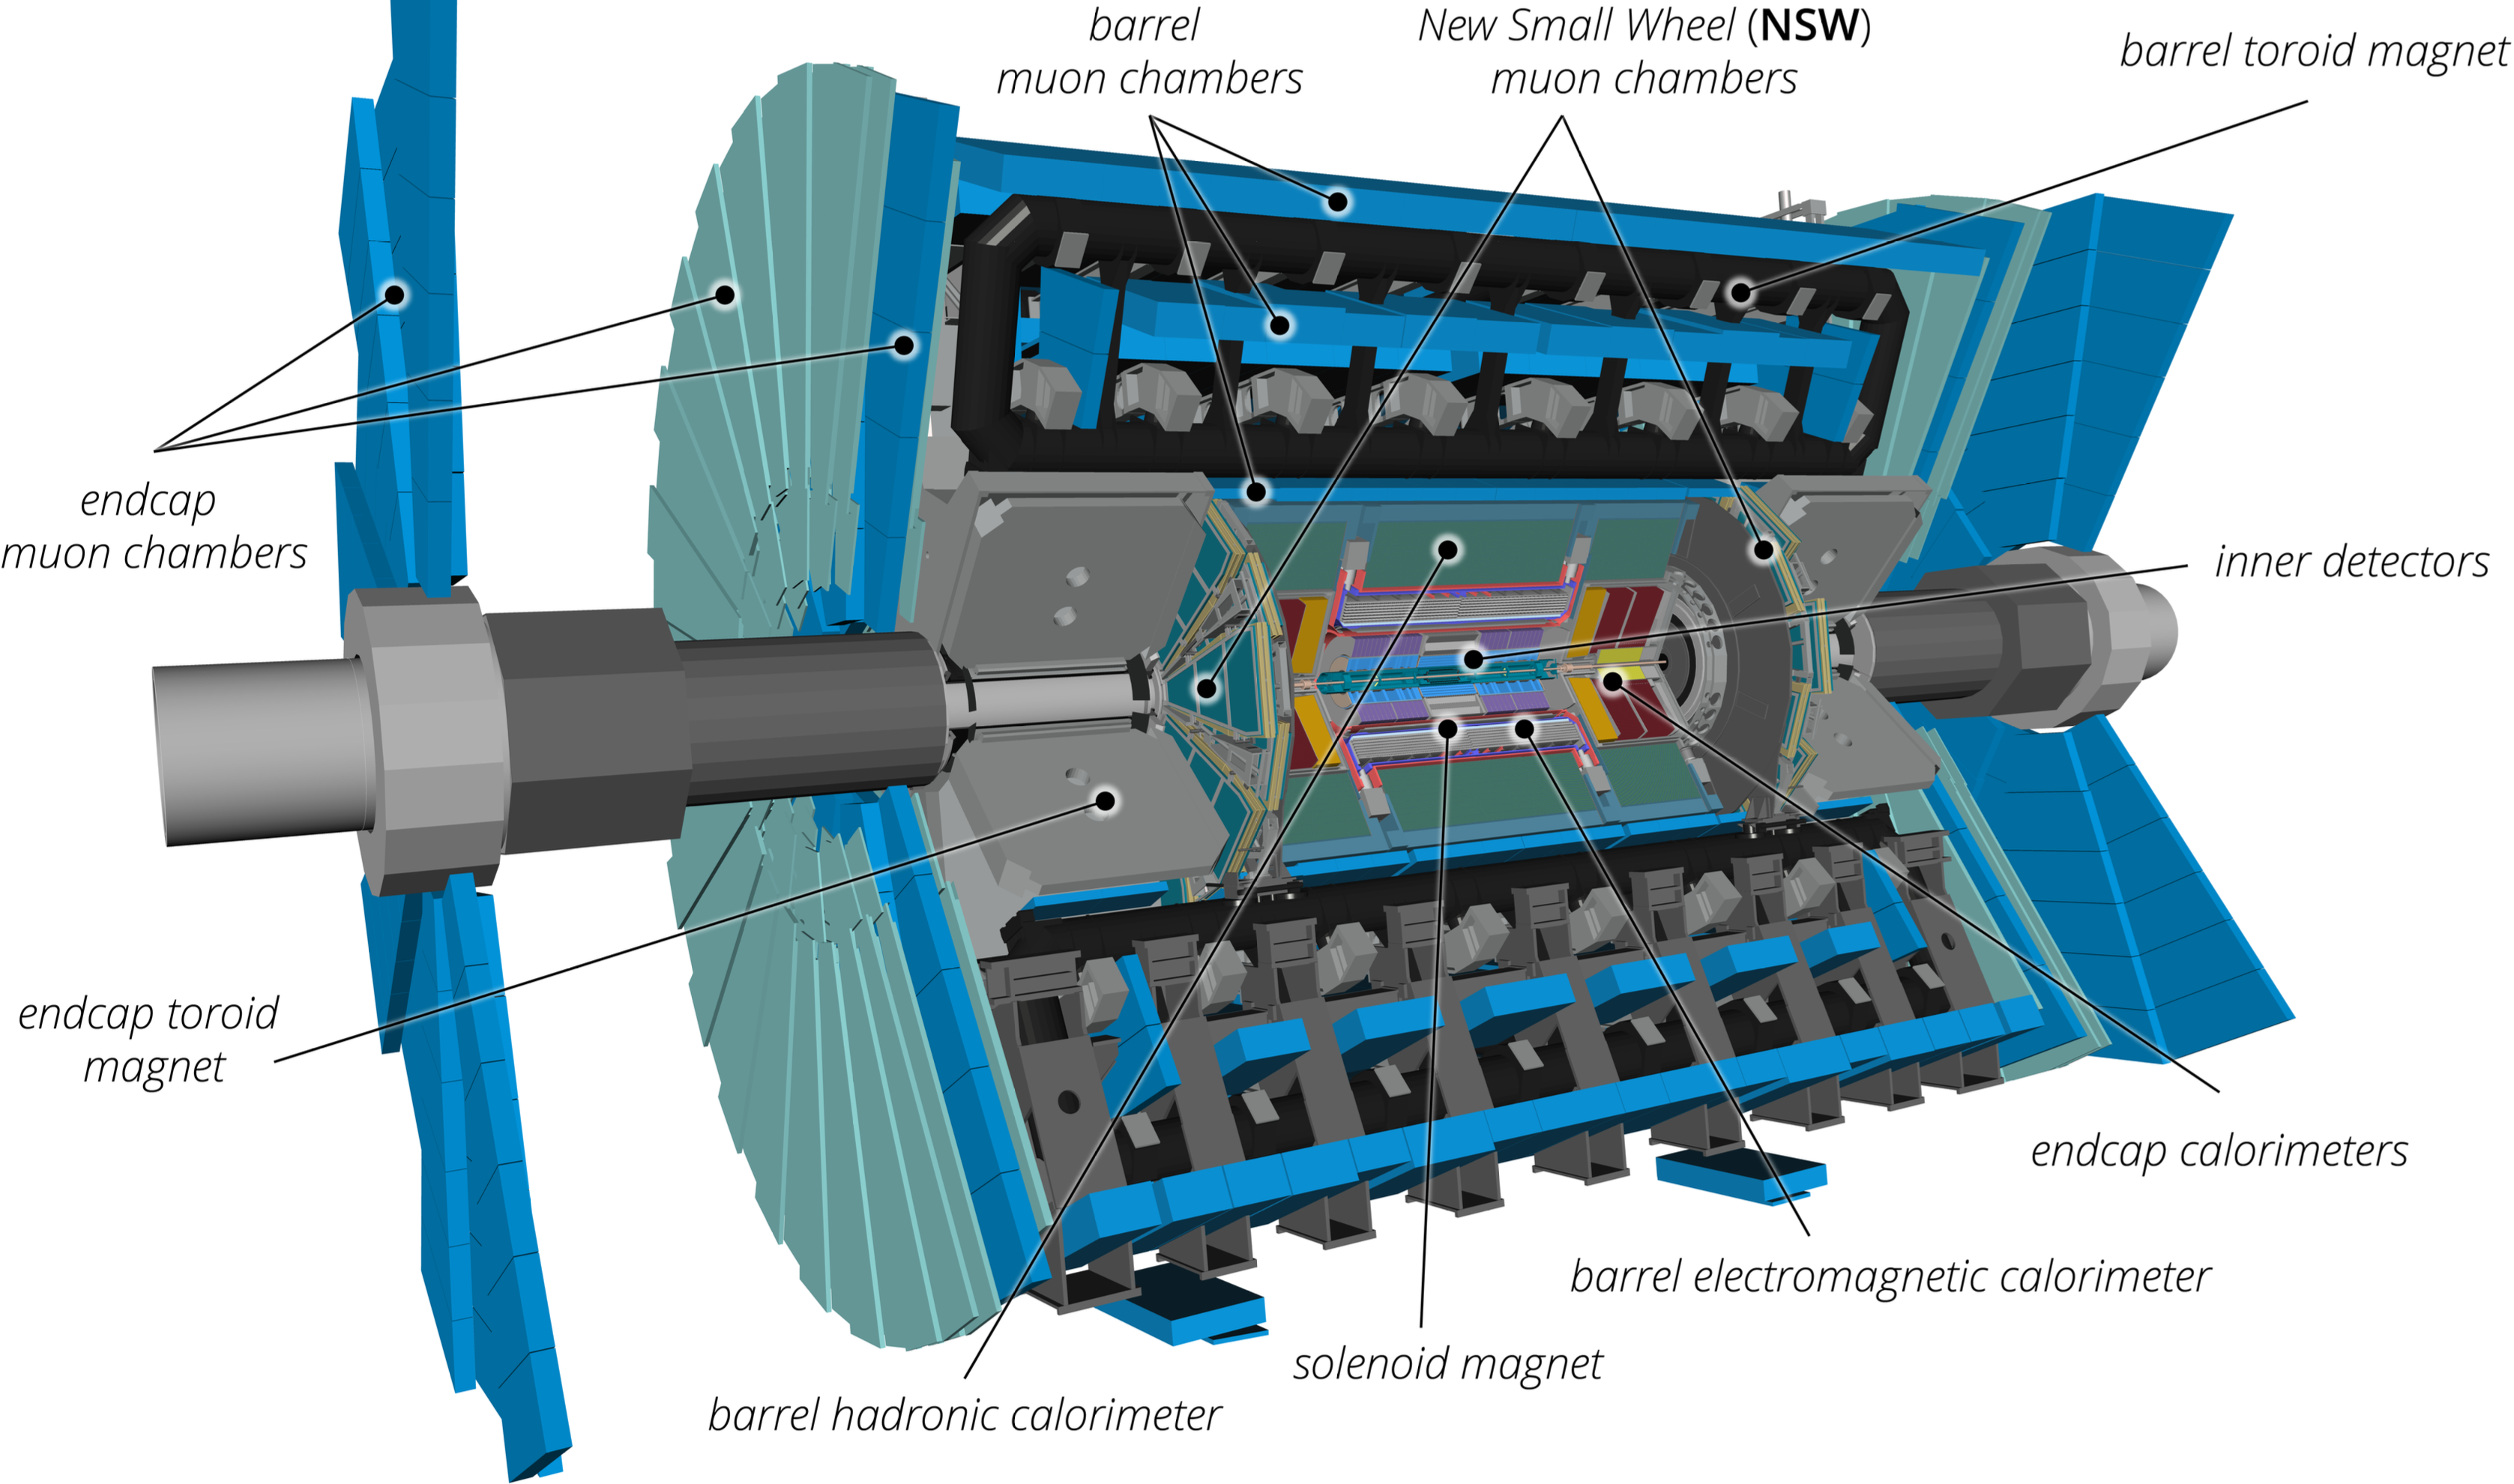
\includegraphics[width=1.0\textwidth]{ATLAS-cutaway-run3.png}
        \caption{Cut-away view of the Run 3 configuration of the ATLAS detector indicating the locations of the larger detector sub-systems, taken from~\cite{GENR-2019-02}}.
        \label{fig:ATLAS_cutaway_run3}
    \end{figure}
    Its diverse array of sophisticated sub-detectors captures and 
    analyses the particles produced in high-energy collisions. The conceptual design of 
    ATLAS began in the early 1990s, with the official Letter of Intent submitted 
    in 1992~\cite{ATLAS-TDR-LOI} and the Technical Proposal in 1994~\cite{ATLAS-TDR-Proposal}. 
    Construction commenced in the late 
    1990s, leading to the installation of the detector in its cavern by 2007. The 
    first proton-proton collisions were recorded in 2009. Over the years, ATLAS has undergone several 
    upgrades to enhance its performance and accommodate increasing collision 
    rates and energies. ATLAS comprises several key components designed to work in concert to achieve 
    comprehensive particle detection and analysis:
    \begin{itemize}
        \item Inner Detector (ID): This component provides precise tracking of charged particle trajectories and interaction points near the collision vertex. It consists of a high-granularity silicon Pixel detector, a Semiconductor Tracker (SCT), and a Transition Radiation Tracker (TRT).
        \item Calorimeters: These measure the energy of particles by absorbing them. The electromagnetic calorimeter detects electrons and photons, while the hadronic calorimeter measures the energy of hadrons. The ATLAS calorimeters use two sampling technologies: liquid argon (LAr) for the electromagnetic calorimeters and all endcap and forward calorimeters, and scintillating tiles for hadron calorimetry in the central region.
        \item Muon Spectrometer: Located outside the calorimeters, this system detects and measures muons, which are minimally ionising particles that penetrate the inner detector and calorimeters. It is based on the magnetic deflection of muon tracks in a large superconducting air-core toroidal magnet system.
        \item Forward Detectors: Comprised of four sub-detectors, the forward detectors play critical roles in measuring luminosity, studying diffractive events, and characterising the centrality~\cite{HION-2010-01} of heavy-ion collisions.
        \item Trigger and Data Acquisition (TDAQ) System: This system selects events of interest based on distinguishing characteristics and reads them out for further offline processing. It consists of the Level-1 Trigger (L1) and the High-Level Trigger (HLT), along with the Data Acquisition system that transports data from sub-detector electronics to offline processing.
    \end{itemize}
    The ATLAS detector has been continuously upgraded to maintain its performance under the increasingly challenging 
    conditions of the LHC. The Phase-I upgrades~\cite{ATLAS-TDR-20,ATLAS-TDR-22,ATLAS-TDR-23,ATLAS-TDR-24}, 
    implemented during LS2 from 2019 to 2022, included improvements to the detector subsystems and their electronics to withstand the high interaction rates expected 
    in Run 3 and beyond. These upgrades focused on enhancing the trigger system, increasing precision tracking, 
    and improving calorimetry and muon detection capabilities. In recent years, the LHC has achieved higher collision 
    energies and luminosities, necessitating further upgrades to the ATLAS detector. 
    The Run 3 configuration, for example, includes new LAr Calorimeter digital trigger electronics, 
    an upgraded Muon Spectrometer with new small wheels (NSWs), and enhanced TDAQ systems to handle the increased data rates and complexity. 
    The Phase-II upgrades, planned for the HL-LHC era~\cite{ATLAS-TDR-PhaseII,ATLAS-TDR-25,ATLAS-TDR-26,ATLAS-TDR-27,ATLAS-TDR-28,ATLAS-TDR-29,ATLAS-TDR-30,ATLAS-TDR-31}, 
    will further enhance the detector's capabilities to meet the demands of higher luminosities and energies. 
    These upgrades will include 
    improvements in calorimeters for higher granularity and faster readout electronics to handle higher collision rates,
    a complete replacement of the ID (ITK) that can handle 
    the increased pile-up conditions and radiation dose,
    upgrades to the TDAQ system that can handle date rates up to 1~MHz at Level-0 and 400~kHz at Level-1,
    and an upgraded Muon Spectrometer for better coverage and resolution. 
    In the following sections, we will delve into the key components of the ATLAS detector
    and their functions in particle detection and analysis. 

    \subsection{ATLAS Coordinate System and Kinematic Variables}
        ATLAS uses a right-handed coordinate system with its origin at the nominal 
        interaction point (IP) in the centre of the detector. The axes are defined as follows:
        the z-axis points along the beamline.
        The x-axis points from the IP to the centre of the LHC ring. 
        The y-axis points upwards, perpendicular to the xz-plane.
        Cylindrical coordinates $(r, \phi)$ are used in the transverse plane, where $r$ is the radial 
        distance from the z-axis, and $\phi$ is the azimuthal angle around the z-axis. 
        In hadron-hadron collisions, rapidity ($y$) 
        and pseudorapidity ($\eta$) are used to describe the angle of a particle relative to the beam axis.
        $y$ is defined as:
        \[
        y = \frac{1}{2} \ln \left( \frac{E + p_z}{E - p_z} \right),
        \]
        where \( E \) is the energy of the particle, and \( p_z \) is the component of the momentum along the beam axis.
        $y$ is advantageous because differences in $y$ are invariant under Lorentz 
        boosts along the z-axis, making it a particularly useful variable in hadron collider physics.
        $\eta$ is a simplified version of $y$, used when the particle mass is negligible compared to its momentum. 
        It is defined as:
        \[
        \eta = -\ln \left( \tan \frac{\theta}{2} \right),
        \]
        where \( \theta \) is the polar angle with respect to the beam axis. 
        $\eta$ is commonly used in collider experiments to describe the angular distribution of particles because it is 
        a more convenient variable than $y$ due to its simpler form, and the fact that it is approximately equal to $y$ 
        for relativistic particles.
        The trajectory of a particle is typically described in terms of its transverse momentum (\pt), $\phi$, $\eta$. 
        $\pt$ is particularly important in collider physics because it is invariant under 
        boosts along the beam axis, and it is conserved in particle collisions. It is defined as:
        \[
        \pt = \sqrt{p_x^2 + p_y^2},
        \]
        where \( p_x \) and \( p_y \) are the momentum components in the transverse plane.

    \subsection{Inner Detector}
        The Inner Detector (ID)~\cite{IDET-2010-01,IDET-2013-01,IDET-2015-01} of the ATLAS experiment 
        is a sophisticated component designed to provide 
        precise tracking of charged particles originating from the collisions. A cut-away view of the
        ATLAS Inner Detector is shown in Figure~\ref{fig:ID_cutaway}.
        \begin{figure}[htbp]
            \centering
            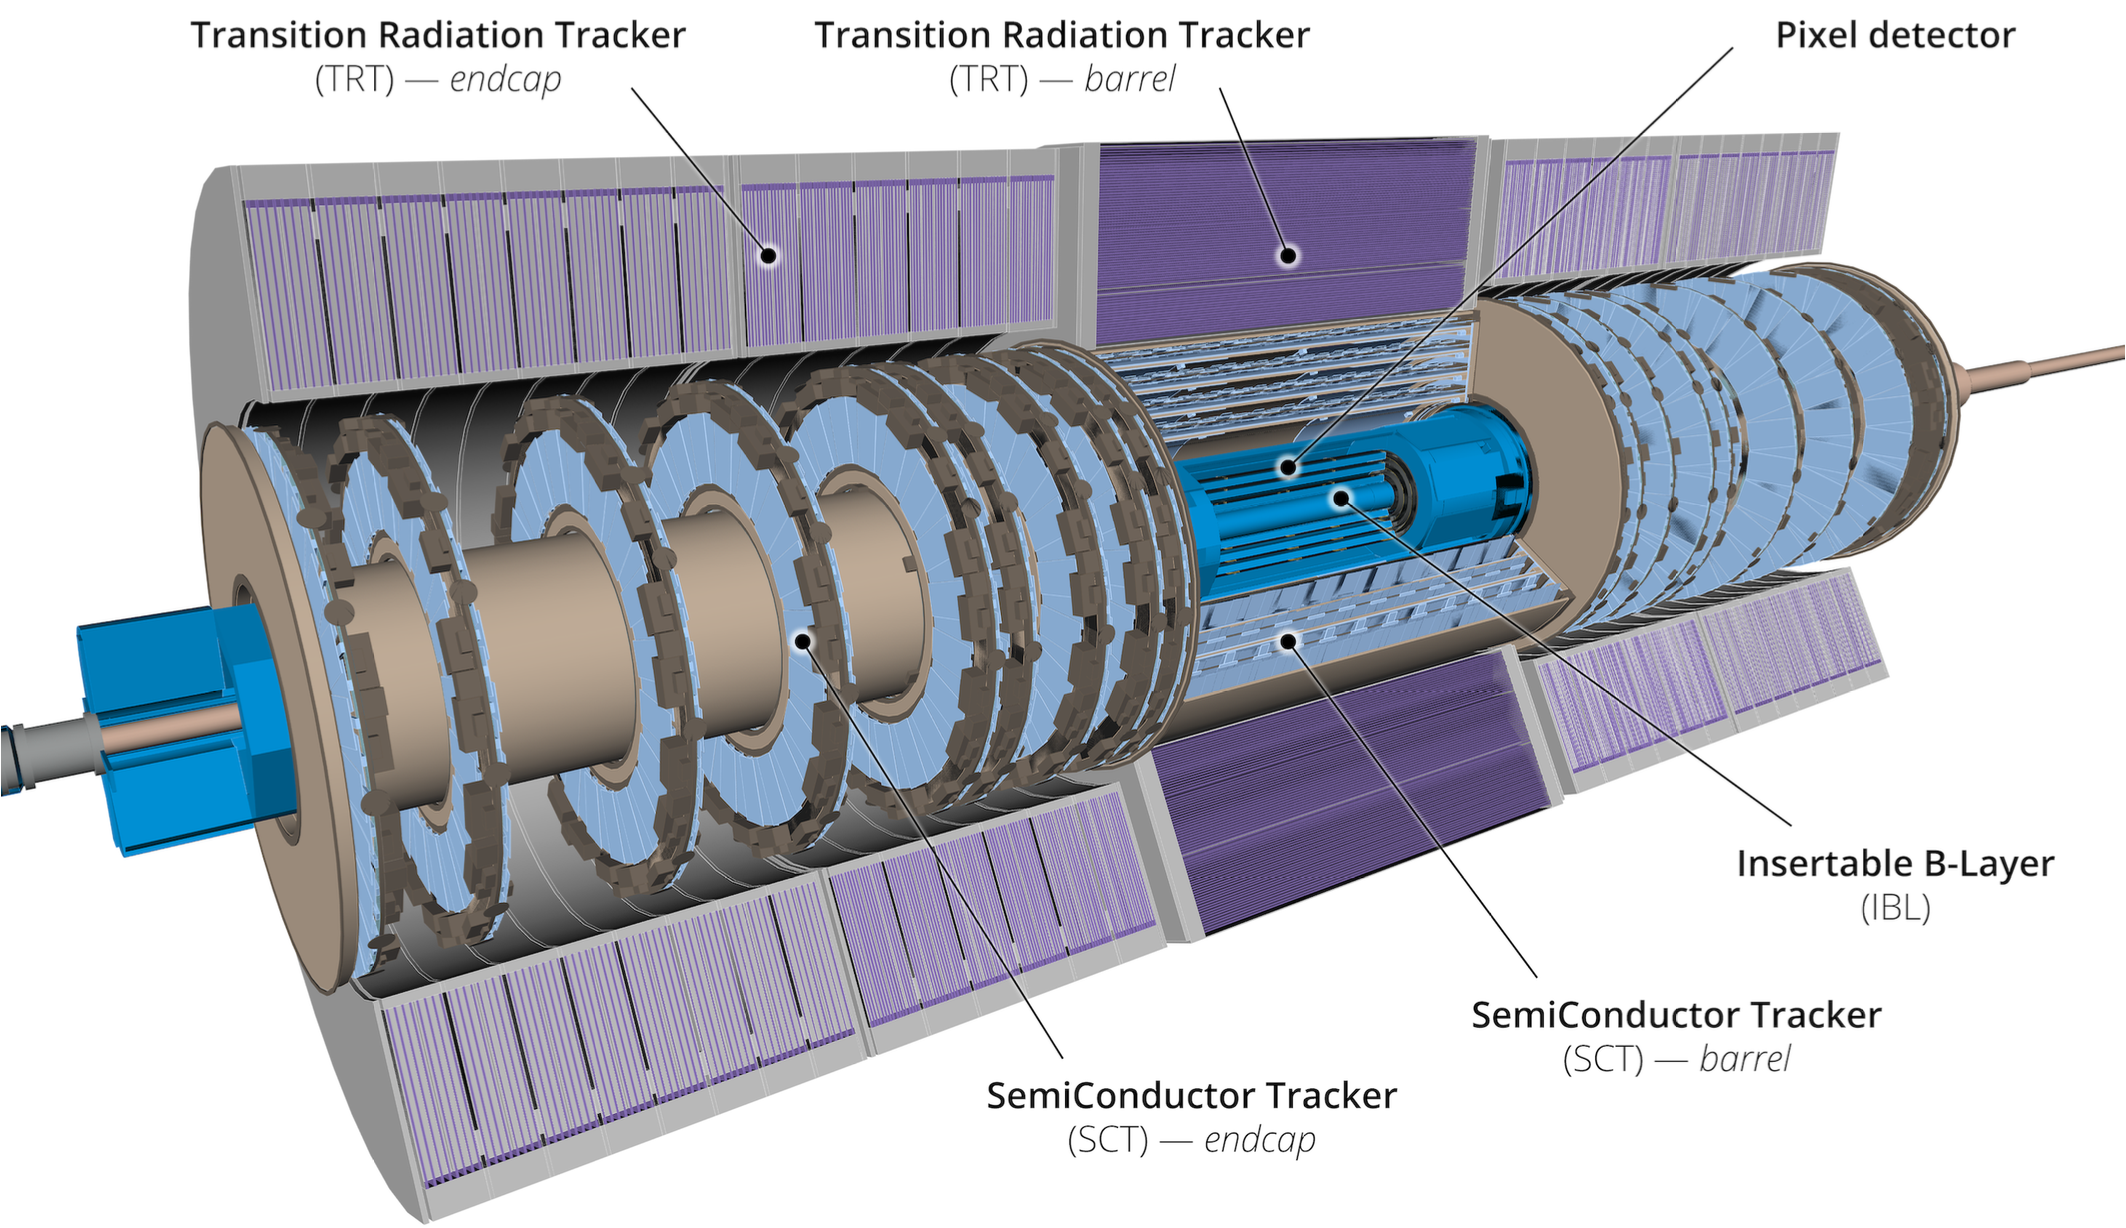
\includegraphics[width=1.0\textwidth]{ATLAS-ID-run3.png}
            \caption{Cut-away view of the ATLAS Inner Detector showing the Pixel Detector, 
                Semiconductor Tracker (SCT), and Transition Radiation Tracker (TRT), taken from~\cite{GENR-2019-02}.}
            \label{fig:ID_cutaway}
        \end{figure}
        The ID is crucial for reconstructing particle trajectories, measuring momenta, and identifying primary and 
        secondary vertices. The design and configuration of the ID have evolved to meet the increasing 
        demands of the LHC. Higher pile-up conditions and radiation levels expected in Run 2 and Run 3
        have necessitated upgrades to the ID to maintain its performance and reliability.
    
        The ID is immersed in a 2~T axial magnetic field generated by a central solenoid, 
        extending over a length of 5.3 meters with a diameter of 2.5 meters~\cite{ATLAS-TDR-06}. The ID covers the 
        pseudorapidity range $|\eta| < 2.5$ and is composed of three primary sub-systems: 
        the Pixel Detector, 
        the Semiconductor Tracker (SCT), 
        and the Transition Radiation Tracker (TRT).
        \begin{itemize}
            \item Pixel Detector~\cite{ATLAS-TDR-11}: The Pixel Detector provides the highest granularity tracking close to the 
            interaction point. It consists of three barrel layers and three endcap discs on each side, with an 
            additional fourth inner layer known as the Insertable B-Layer (IBL)~\cite{PIX-2018-001} installed during LS1. 
            The pixels have dimensions of $50~\si{\um} \times 400~\si{\um}$, 
            with the IBL featuring even finer segmentation at $50~\si{\um} \times 250~\si{\um}$. 
            This system typically provides four precise position 
            measurements per track, aiding in pattern recognition, accurate vertex reconstruction and b-tagging.
            \item Semiconductor Tracker (SCT)~\cite{SCTD-2019-01}: Surrounding the Pixel Detector, the SCT extends the tracking 
            capabilities further from the interaction point. It consists of four barrel layers and nine endcap 
            discs on each side. The SCT uses silicon microstrip technology, with strips oriented to measure both 
            radial and azimuthal coordinates, providing eight measurements per track. The strip pitch is approximately 
            80~$\si{\um}$, allowing for high-resolution tracking over a larger volume than the Pixel Detector.
            \item Transition Radiation Tracker (TRT)~\cite{IDET-2015-01}: The outermost component of the ID, the TRT,
            consists of layers of straw tubes interleaved with radiators that induce transition radiation 
            when traversed by high-energy electrons. The TRT covers range $|\eta| < 2.0$, offering additional particle identification 
            capabilities through the measurement of energy deposition in the straws.
        \end{itemize}
        Several upgrades and enhancements have been implemented in the ID for Run 3 to handle the increased 
        collision energy of 13.6 TeV and the higher luminosity conditions. These include improvements in 
        detector readout electronics, data acquisition systems, and the integration of new cooling systems 
        to maintain optimal operational conditions under the high-radiation environment anticipated during Run 3.
        The precision tracking performance of the ID has been pivotal in enabling ATLAS to achieve its broad 
        physics objectives, from detailed studies of the Higgs boson to searches for new physics phenomena. 
        \begin{figure}[htbp]
            \centering
            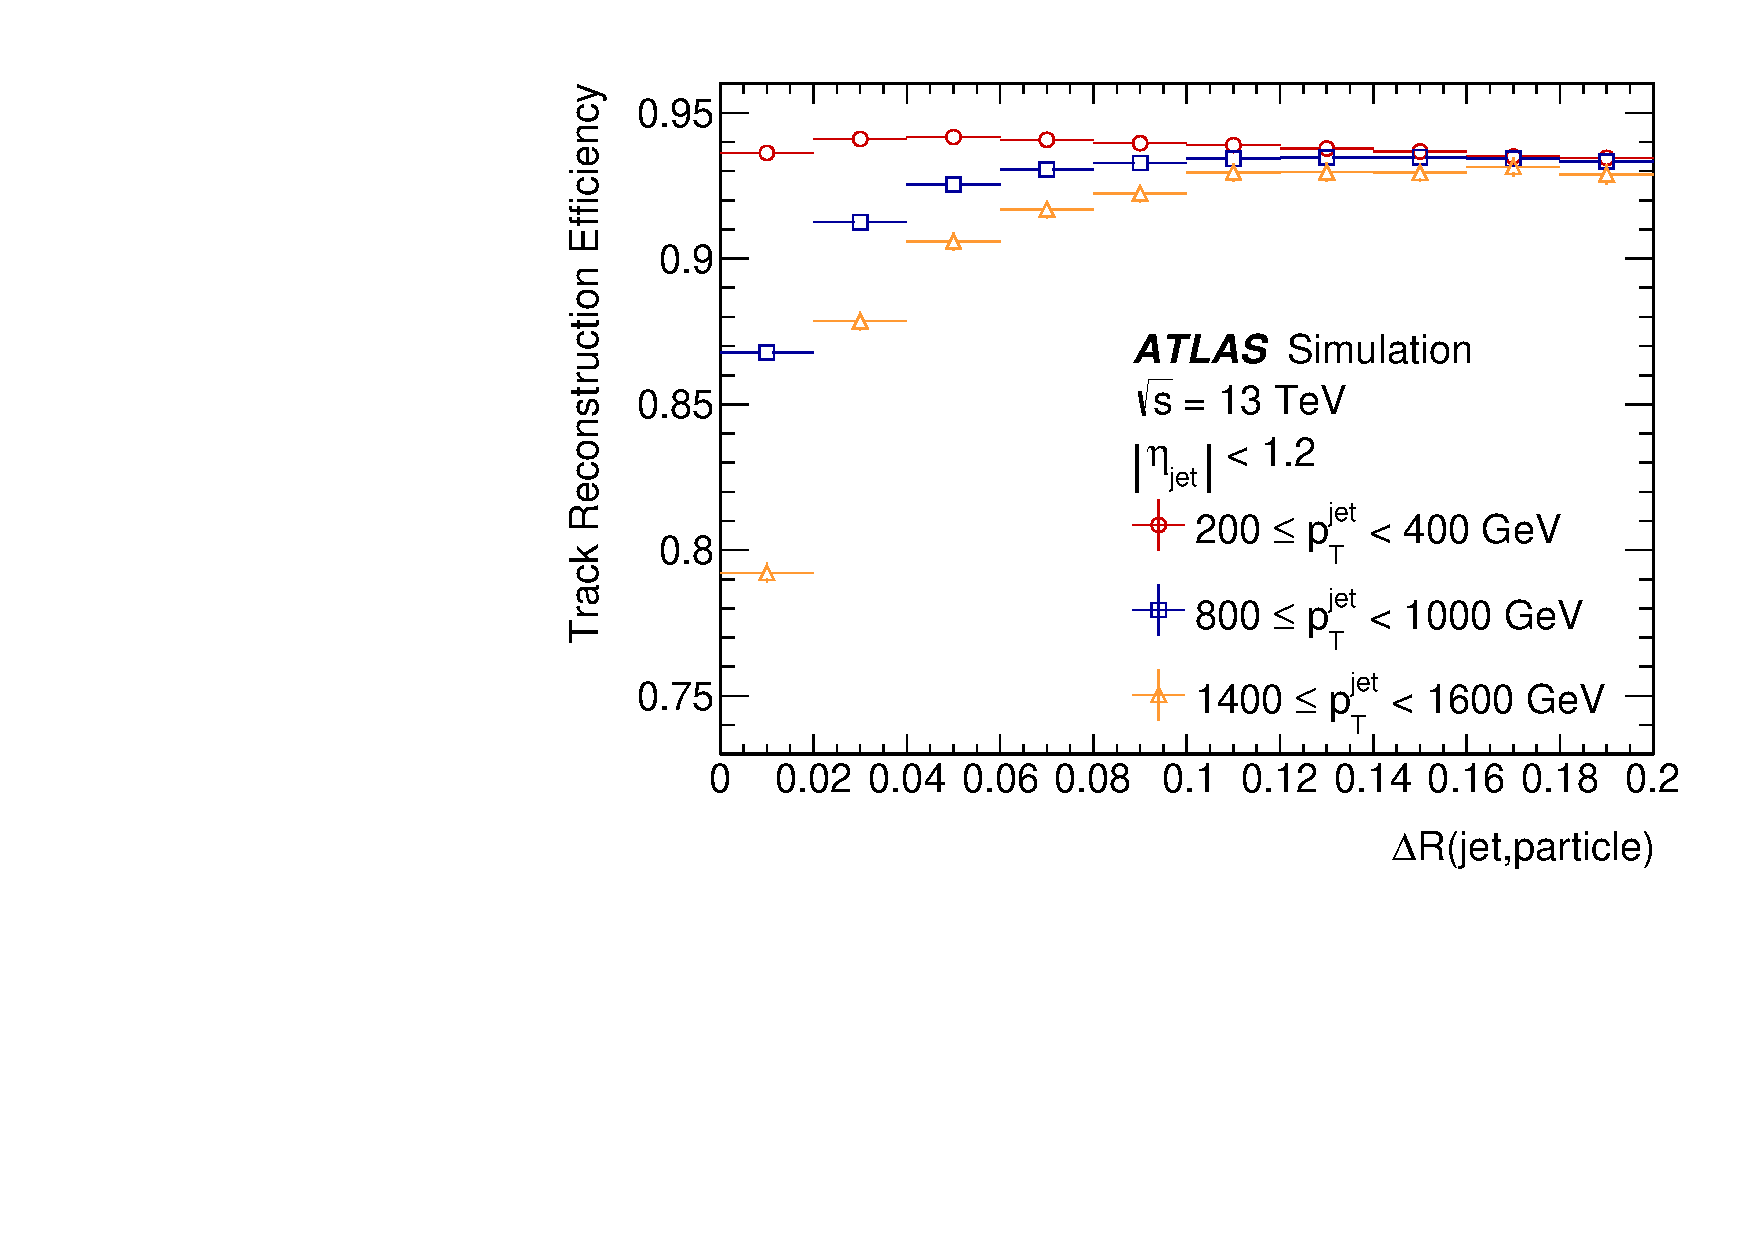
\includegraphics[width=0.495\textwidth]{trk_eff_loeta.pdf}
            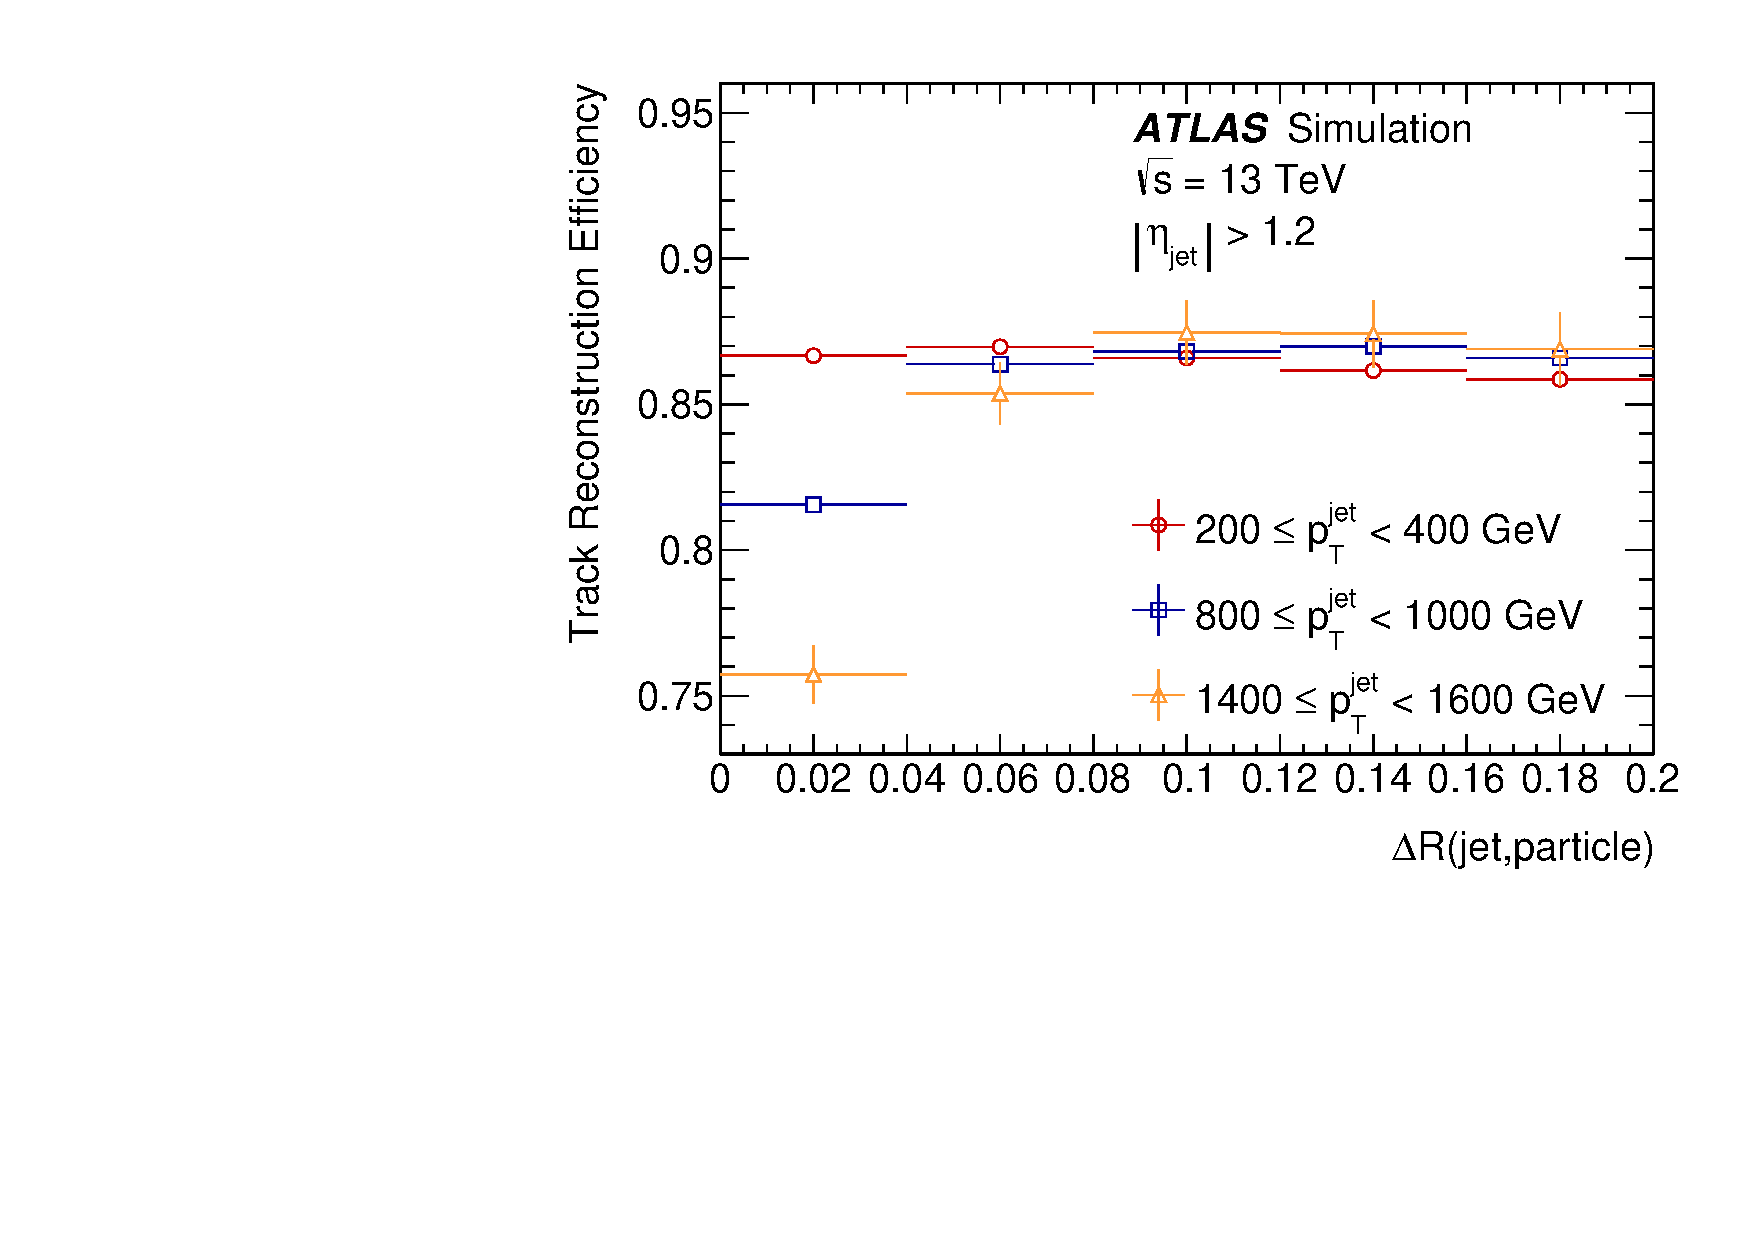
\includegraphics[width=0.495\textwidth]{trk_eff_hieta.pdf}
            \caption{
                The efficiency to reconstruct charged primary particles in jets with (left) $|\eta|< 1.2$ and (right) $|\eta|> 1.2$ is
                shown as a function of the angular distance of the particle from the jet axis for various jet $\pt$ for simulated dijet
                MC events. These figures are taken from~\cite{PERF-2015-08}.
            }
            \label{fig:trk_eff}
        \end{figure}
    \subsection{Calorimeters}
        The ATLAS calorimeter system measures the energies and positions of charged and
        neutral particles through interleaved absorber and active layers out to $|\eta| < 4.9$.
        The calorimeter system is divided into two main types of calorimeters: 
        the Liquid Argon~(LAr)~\cite{ATLAS-TDR-02} calorimeters and the 
        Tile calorimeters~\cite{ATLAS-TDR-03}, each optimised for different aspects of calorimetry.
        A cut-away view of the ATLAS calorimeter system is shown in Figure~\ref{fig:Calo_cutaway}.
        \begin{figure}[htbp]
            \centering
            \includegraphics[width=1.0\textwidth]{ATLAS-calo-run3.png}
            \caption{Cut-away view of the ATLAS calorimeter system showing the Liquid Argon (LAr) 
                calorimeters and the Tile calorimeters, taken from~\cite{GENR-2019-02}.}
            \label{fig:Calo_cutaway}
        \end{figure}
        \subsubsection{Liquid Argon Calorimeters}
            The Liquid Argon (LAr) calorimeter systems are responsible for high-precision measurements 
            of the energy deposited by electrons, photons, and hadrons. 
            They employ a sampling technology, where layers of absorbing material are 
            interleaved with active liquid argon layers. This design allows the calorimeters to measure 
            the energy of particles by sampling their energy loss as they pass through the detector.
            It is divided into several subsystems, each serving a specific purpose:
            \begin{itemize}
            \item LAr Electromagnetic Barrel Calorimeter (EMB): this subsystem covers the central region of the detector and is designed to measure the energy of electrons and photons with high precision. The EMB uses lead absorbers and liquid argon as the active medium.
            \item LAr Electromagnetic Endcap Calorimeter (EMEC): extending the coverage to the forward regions, the EMEC provides similar functionality to the EMB but for particles emitted at smaller angles relative to the beamline.
            \item LAr Hadronic Endcap Calorimeter (HEC): located behind the EMEC, the HEC measures the energy of hadrons. It uses copper absorbers and liquid argon, providing complementary measurements to the Tile calorimeters in the central region.
            \item LAr Forward Calorimeter (FCal): positioned in the very forward regions, the FCal is designed to measure the energy of particles at small angles to the beamline, using a combination of tungsten and liquid argon.
            \end{itemize}

        \subsubsection{Tile Calorimeters}
            The Tile calorimeter system is designed to measure the energy of hadrons and jets in the central 
            region of the detector. It consists of steel absorbers interleaved with scintillating tiles. 
            The Tile calorimeter is segmented into three barrel structures. 
            The Central Barrel (CB) covers the central region around the interaction point and the Extended
            Barrels (EB), positioned on either side of the central barrel to extend the coverage.
            The Tile calorimeter also uses a sampling technique, with the scintillating tiles producing light when 
            charged particles pass through them. This light is then collected by photomultiplier tubes (PMTs) and 
            converted into electronic signals that are processed to determine the energy of the incident particles.
        \subsubsection{Calorimeter Upgrades for Run 3}
            The ATLAS calorimeter system has undergone significant upgrades to enhance its performance for Run 3~\cite{ATLAS-TDR-22}. 
            These upgrades include improvements to the readout electronics and the implementation of a new digital 
            trigger system for the LAr calorimeters. These enhancements are aimed at handling the higher collision 
            energy and increased luminosity expected during Run 3, ensuring that the calorimeter system continues 
            to provide precise measurements under more demanding conditions.
            The calorimeters are critical for a wide range of physics analyses, including the identification and measurement 
            of electrons, photons, taus, and jets, as well as the calculation of missing transverse energy (\MET). 
    \subsection{Muon Spectrometer}
        The ATLAS Muon Spectrometer (MS)~\cite{ATLAS-TDR-10} forms the large outer part of the ATLAS detector, designed 
        to detect charged particles exiting the barrel and endcap calorimeters in the pseudorapidity range \(|\eta| < 2.7\). 
        The primary goal of the MS is to 
        provide precise momentum measurements and trigger capabilities for muons. A cut-away view of the
        ATLAS Muon Spectrometer is shown in Figure~\ref{fig:MS_cutaway}.
        \begin{figure}[htbp]
            \centering
            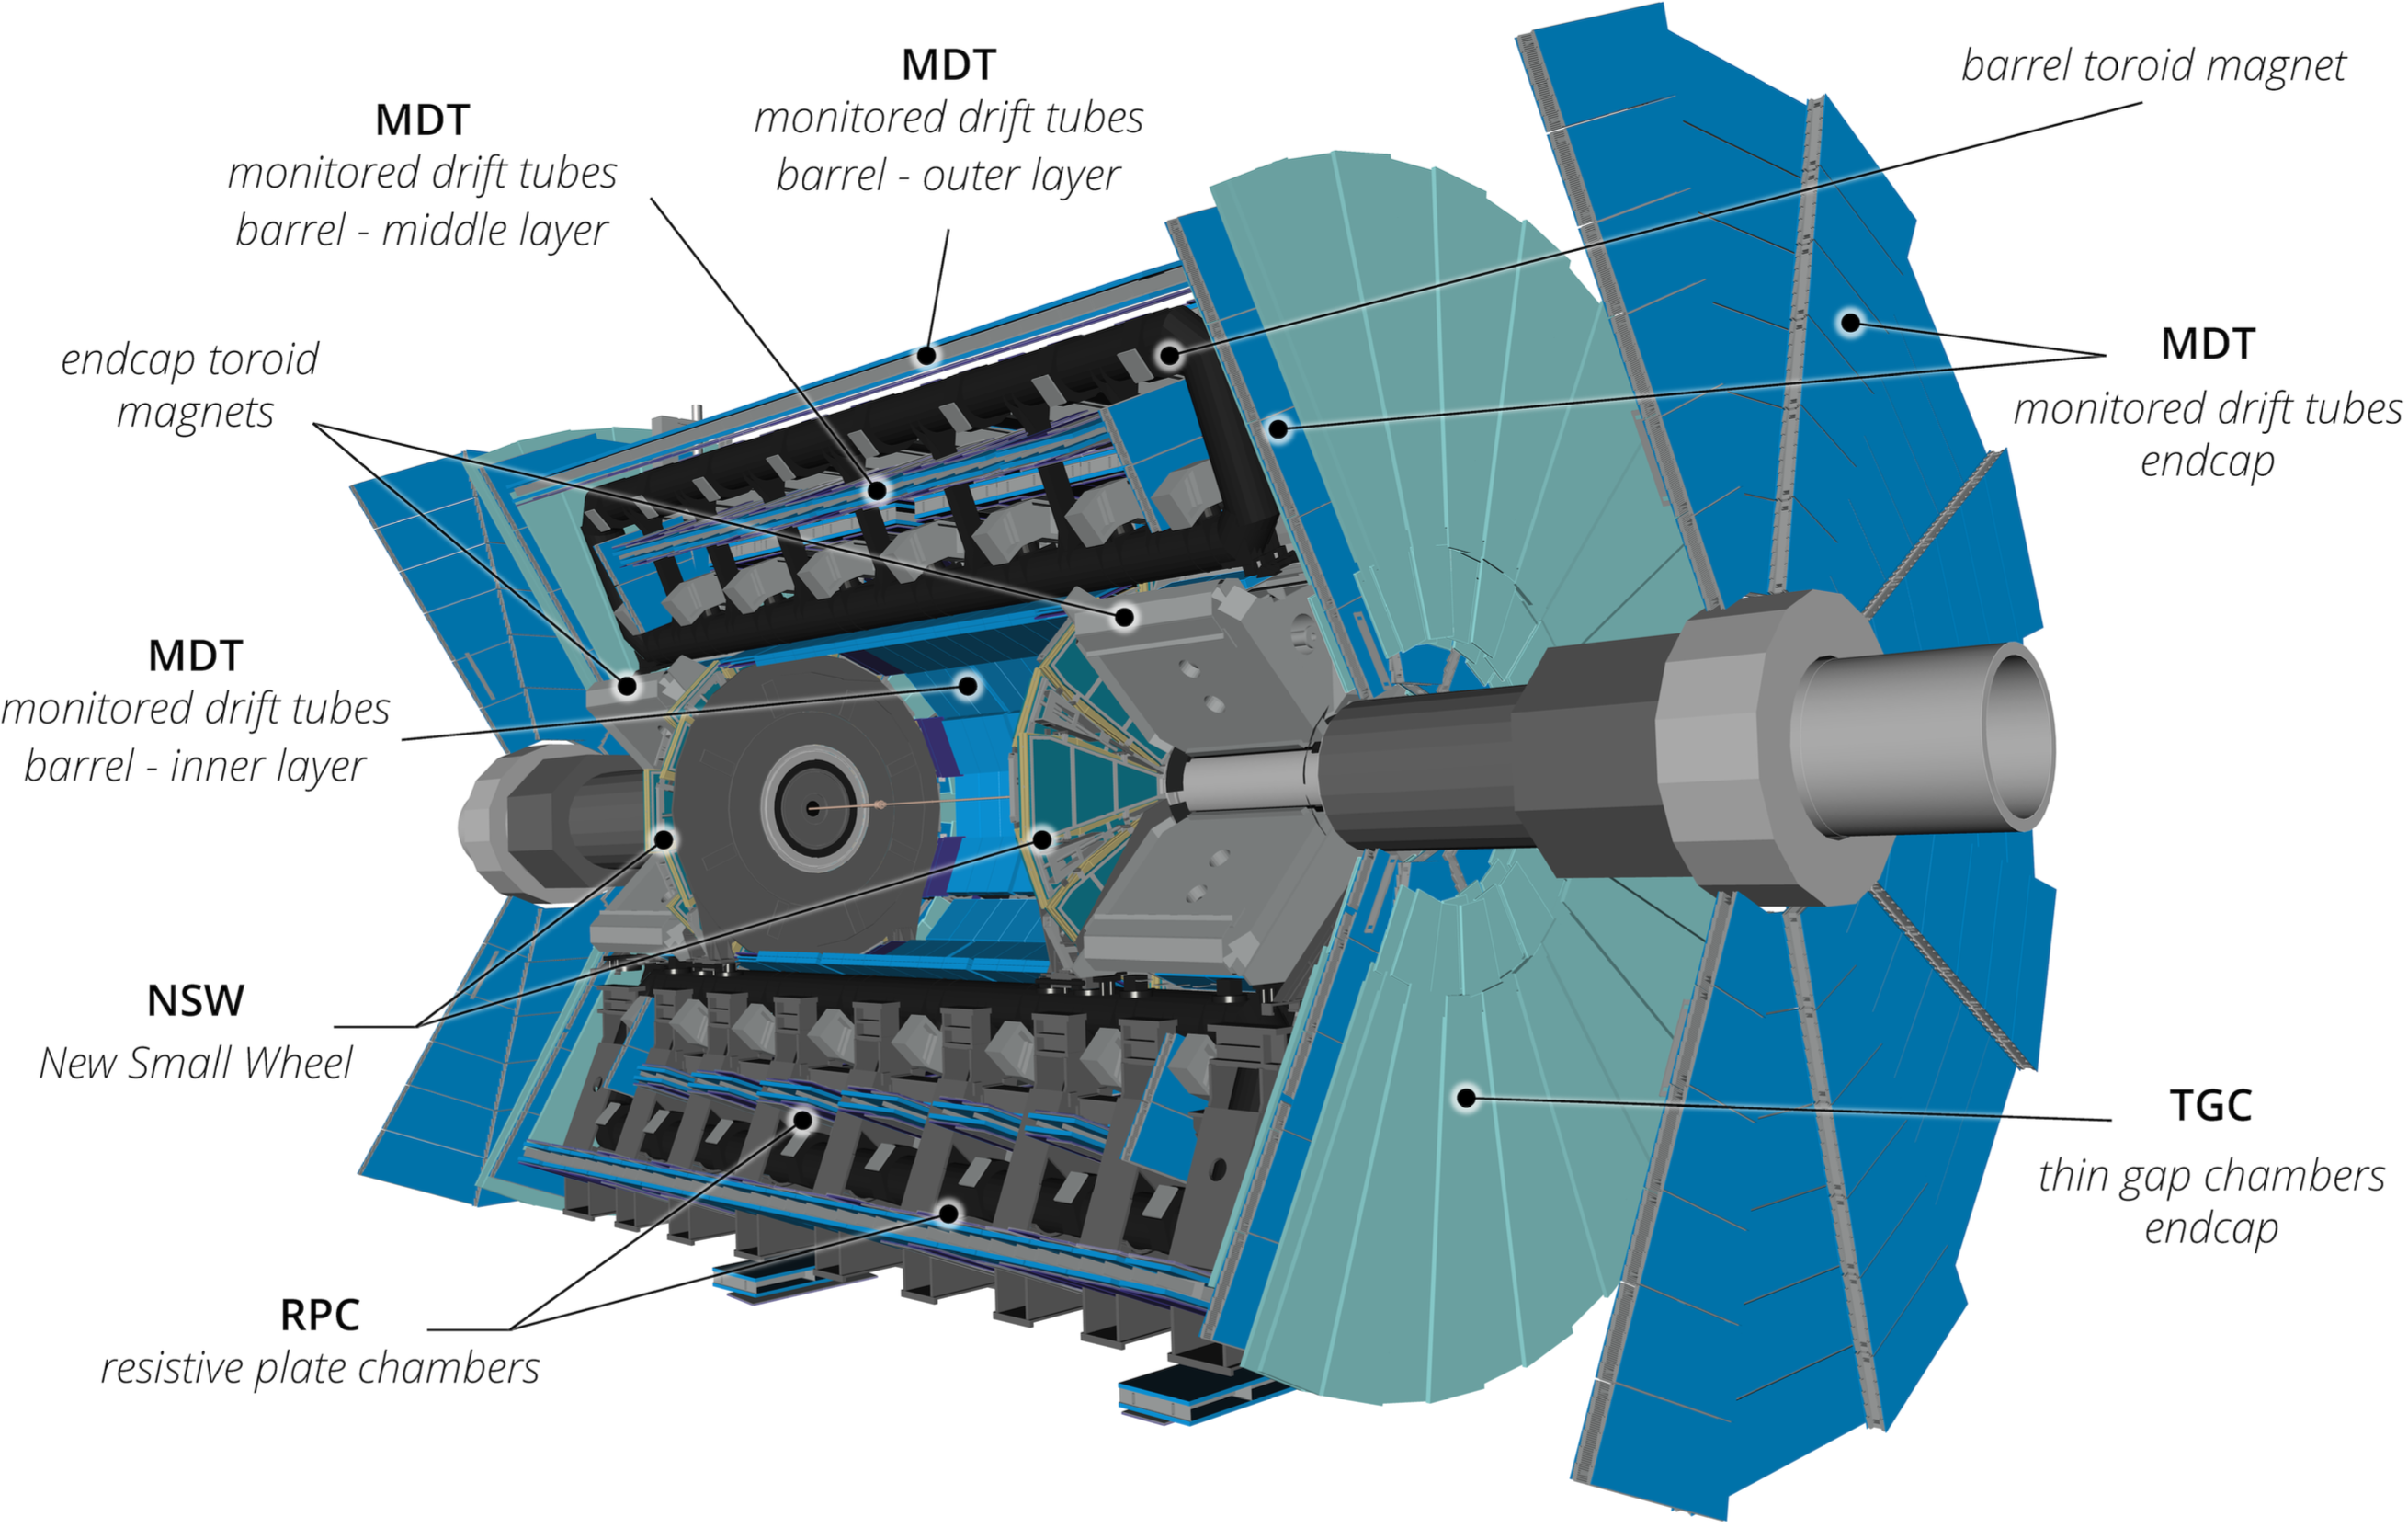
\includegraphics[width=1.0\textwidth]{ATLAS-MS-run3.png}
            \caption{Cut-away view of the ATLAS Muon Spectrometer, taken from~\cite{GENR-2019-02}.}
            \label{fig:MS_cutaway}
        \end{figure}

        The MS is composed of several layers of different detector technologies, all optimised for 
        tracking muons through the strong magnetic fields generated by the ATLAS toroidal magnet system. 
        The MS is divided into three main regions: the barrel, the endcaps, and the transition regions 
        between the barrel and endcaps.
        \begin{itemize}
        \item Barrel Region: the barrel region covers the central part of the detector (\(|\eta| < 1.0\)) and consists of three concentric cylindrical layers known as stations. These stations are equipped with Monitored Drift Tubes (MDTs) for precision tracking and Resistive Plate Chambers (RPCs) for triggering.
        \item Endcap Regions: the endcaps extend the coverage of the MS to higher pseudorapidities (\(1.0 <|\eta| < 2.7\)). Each endcap consists of three disc-shaped stations. The precision tracking in the endcaps is provided by MDTs and Cathode Strip Chambers (CSCs), while the triggering is primarily handled by Thin Gap Chambers (TGCs).
        \item Transition Regions: these regions (\(1.0 < |\eta| < 1.4\)) require special treatment due to the overlap of the barrel and endcap magnetic fields. 
        \item New Small Wheels (NSWs)~\cite{ATLAS-TDR-20}: equipped with Small-Strip Thin Gap Chambers (sTGCs) and Micromegas detectors, the NSWs improve the resolution and redundancy in the $1.3 < |\eta| < 2.7$ region.
        \end{itemize}
        The MDTs are the primary technology used for precision tracking within the MS. Each MDT chamber 
        contains multiple layers of drift tubes, which measure the time taken for ionisation electrons 
        produced by a traversing muon to reach a central wire. This time measurement allows for precise 
        determination of the muon's trajectory. MDTs cover the entire pseudorapidity range of the MS 
        up to \(|\eta| = 2.7\), providing high-resolution tracking data.
        RPCs are used in the barrel region for fast muon triggering. They consist of two parallel plates 
        with a high voltage applied across them. When a muon passes through the chamber, it ionises the 
        gas between the plates, creating an electrical signal that is detected and used to generate a 
        trigger. RPCs also provide measurements of the azimuthal coordinate of muon tracks, aiding 
        in the overall reconstruction process.
        TGCs are used in the endcaps for both triggering and precision tracking. Similar to RPCs, 
        TGCs operate by detecting ionisation events caused by traversing muons. They are designed to 
        handle the high particle fluxes present in the endcap regions and are essential for providing 
        rapid trigger signals to the data acquisition system.    
        CSCs are employed in the innermost endcap layers where particle fluxes are highest. They 
        consist of a plane of wires sandwiched between cathode strips. When a muon passes through 
        the chamber, it ionises the gas, and the resulting electrons are collected by the wires, 
        while the ions induce a signal on the cathode strips. This configuration allows for precise 
        two-dimensional tracking.
        The NSWs, installed as part of the Phase-I upgrades, are designed to handle the high particle 
        rates and provide improved precision in the forward region. They utilise two types of 
        detectors: sTGCs and Micromegas. The sTGCs offer fast response times for triggering, while 
        the Micromegas provide high spatial resolution for tracking. The combination of these 
        technologies ensures robust performance in the high-radiation environment expected during Run 
        3 and beyond.
        The MS aims for a stand-alone transverse momentum resolution better than 15\% for 1 TeV tracks, 
        which requires an effective sagitta resolution of about 75 \(\mu\)m over a large detector volume. 
        This precision is achieved through careful design and regular upgrades. For Run 3, the MS has 
        undergone significant enhancements, in addition to NSWs, the MDT readout electronics has been upgraded
        to handle higher data rates and improve overall performance.
        \begin{figure}[htbp]
            \centering
            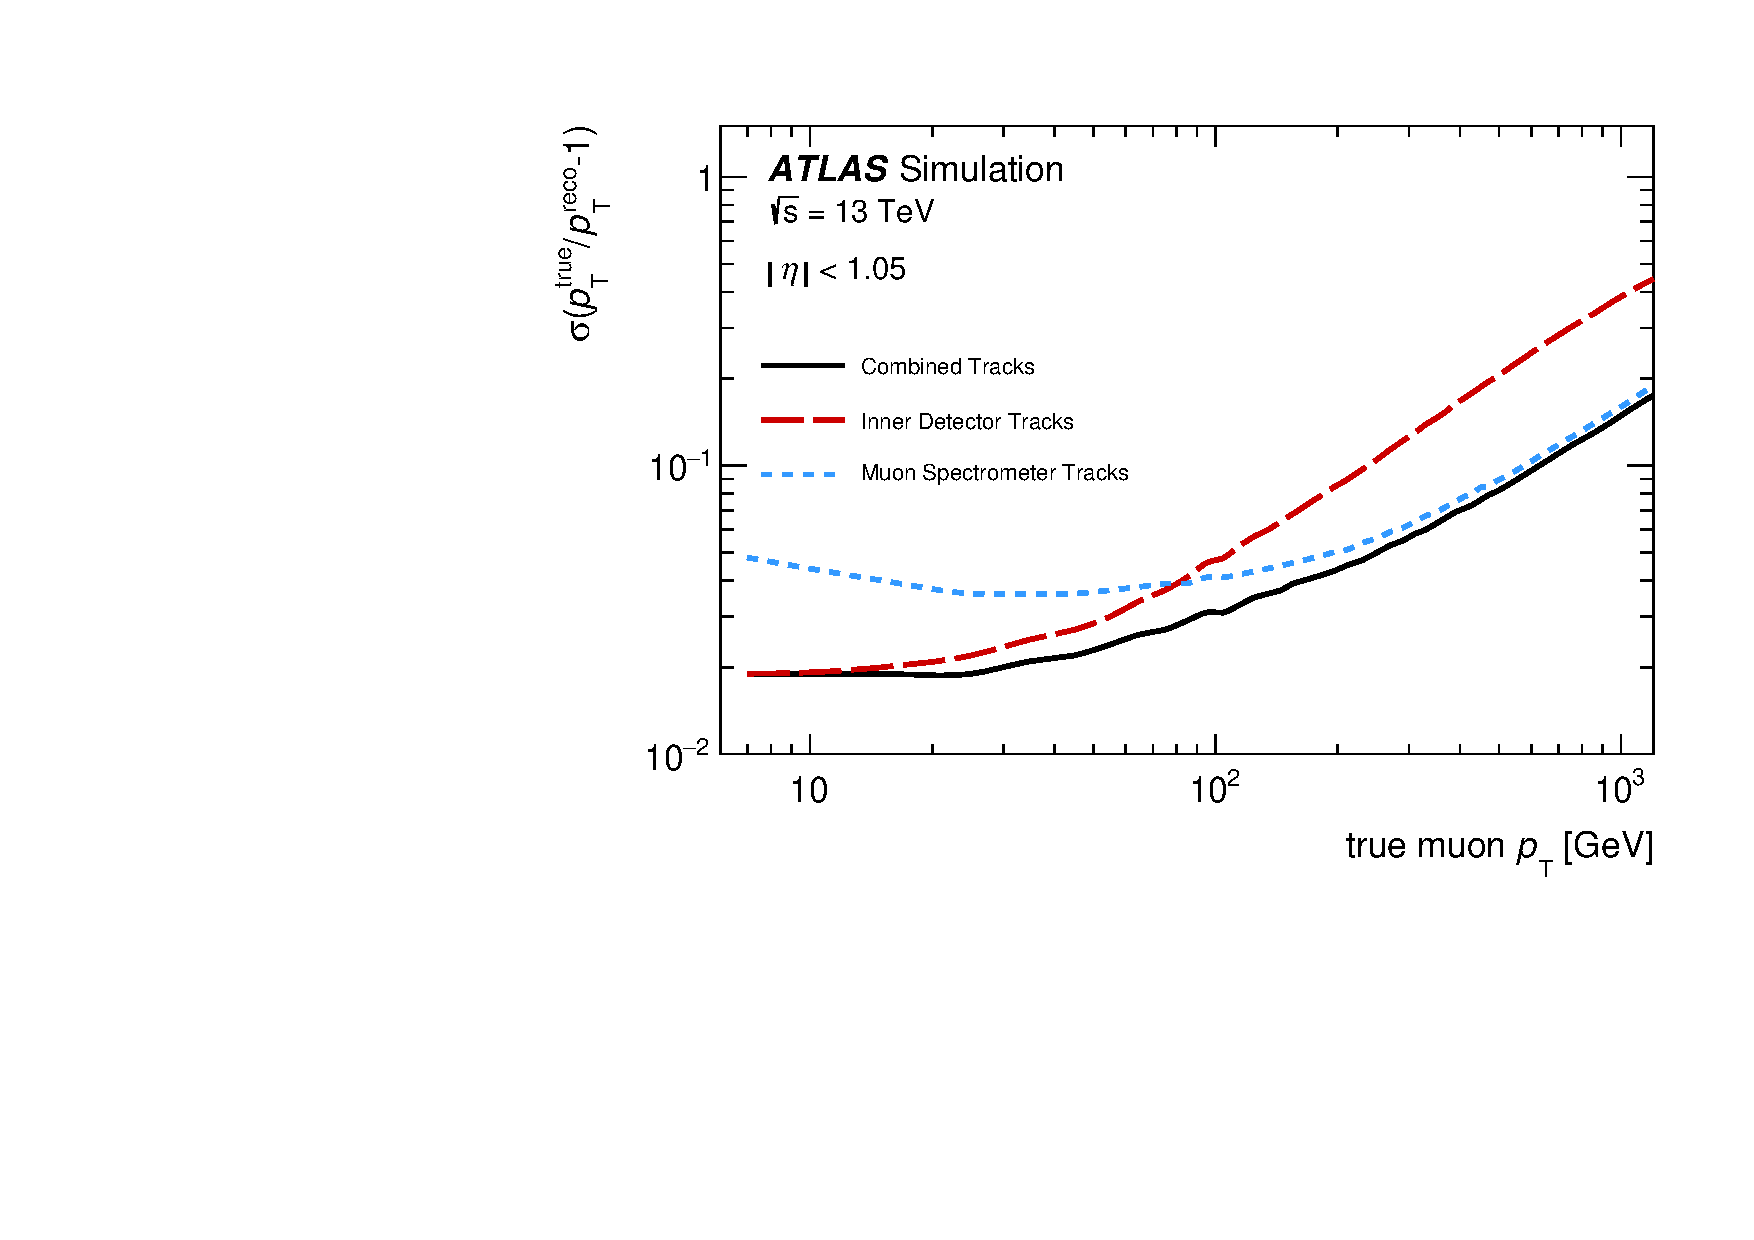
\includegraphics[width=0.495\textwidth]{muon_reco_reso_loeta.pdf}
            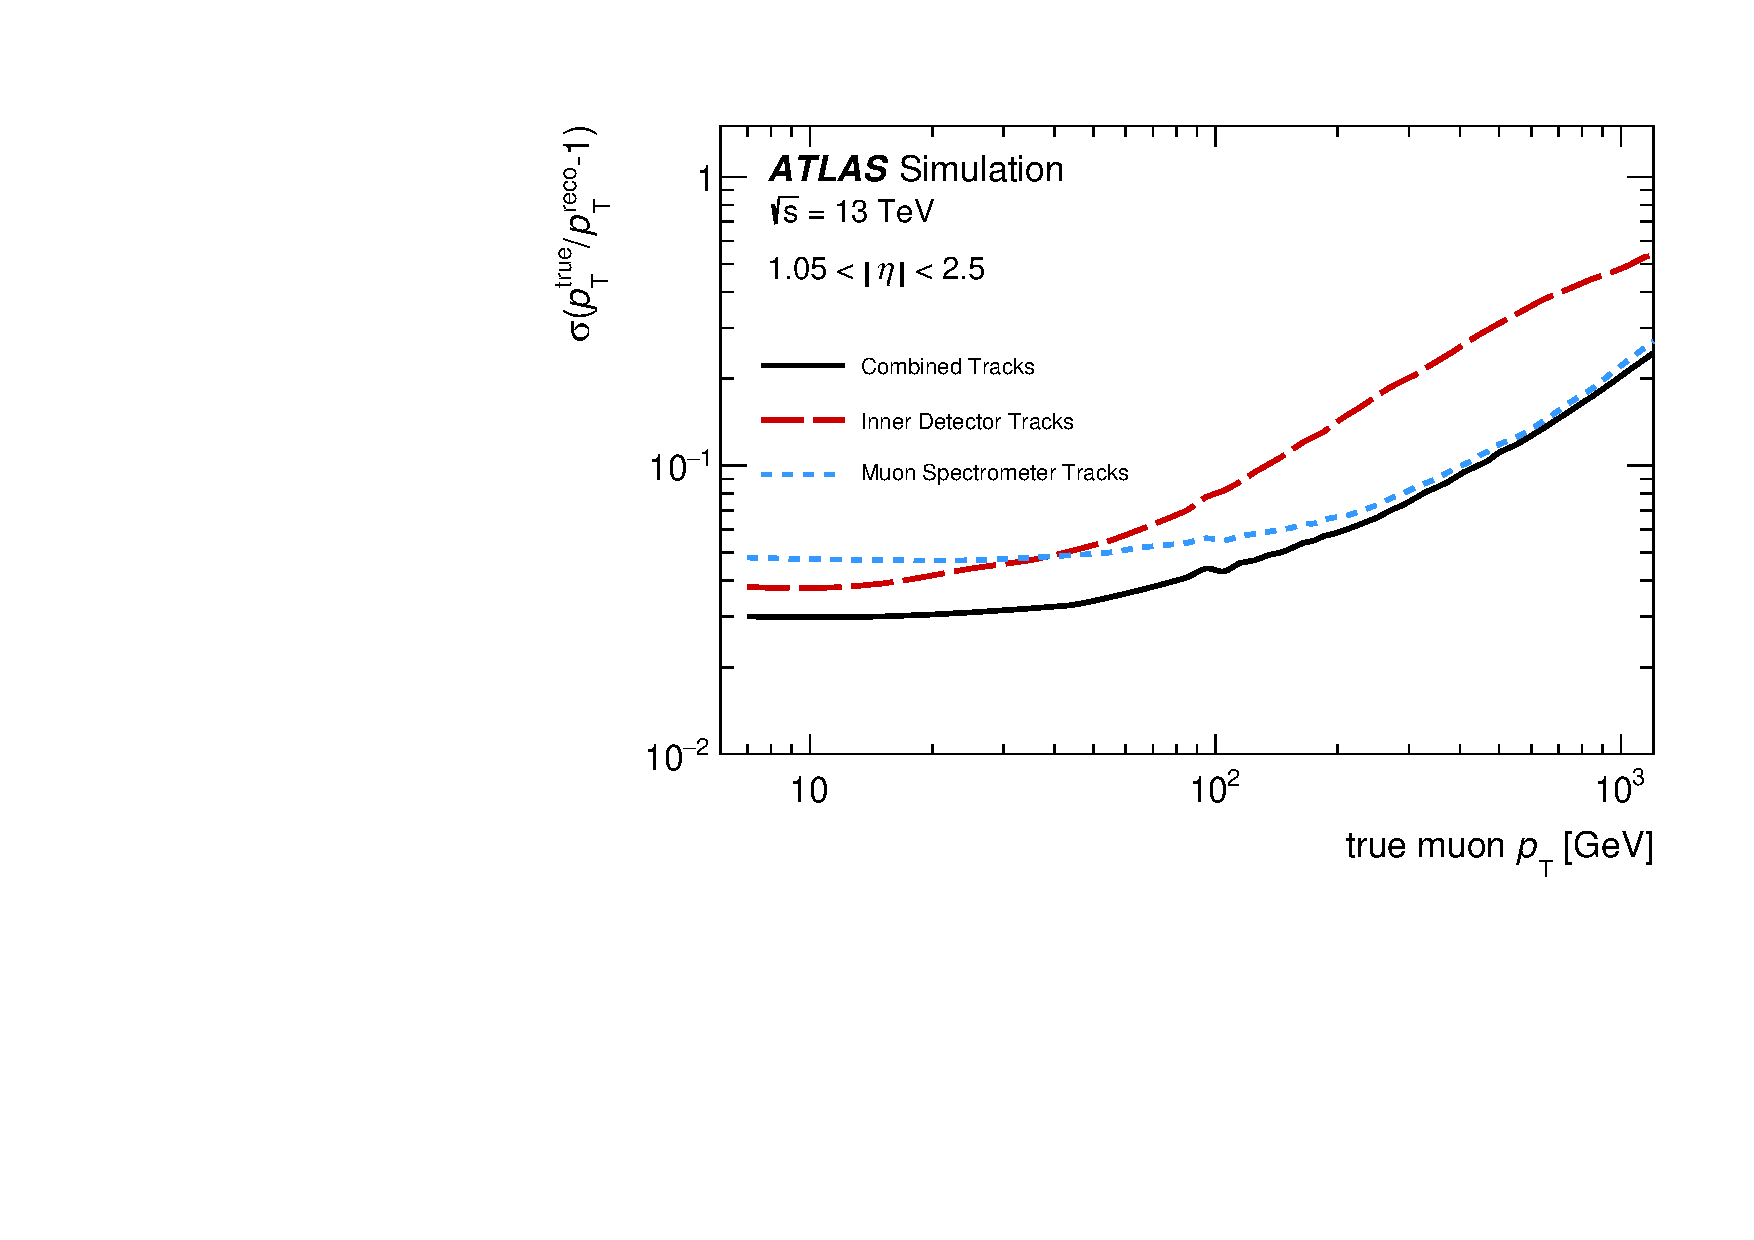
\includegraphics[width=0.495\textwidth]{muon_reco_reso_hieta.pdf}
            \caption{
                Resolution of the muon $\pt$ as obtained from simulation after derivation and application of all correction constants. 
                Muons are selected using the High-$\pt$ Working point. 
                The resolution is shown as a function of the true $\pt$ of the muon for a range from 1 GeV to 2.5 TeV, 
                (left) for muons with $|\eta|<1.05$ and (right) for muons with $|\eta|>1.05$. 
                The resolution lines are obtained by interpolating between points sampled in steps of $\pt$. 
                The continuous lines correspond to the combined momentum, while the dashed lines to that from the ID, and the dotted lines to that of the MS.
                These figures are taken from~\cite{MUON-2022-01}.
            }
            \label{fig:muon_reso}
        \end{figure}
    
    \subsection{Forward Detector}
        The forward detector systems of the ATLAS experiment~\cite{ATLAS-TDR-18} play crucial roles in measuring luminosity, 
        studying diffractive events, and characterising the centrality of heavy-ion collisions. These 
        detectors extend the capabilities of ATLAS by covering the forward regions, providing essential 
        data that complement the central detector systems. Figure \ref{fig:Forward_detectors} shows the
        layout of the forward detectors in the ATLAS experiment.
        \begin{figure}[htbp]
            \centering
            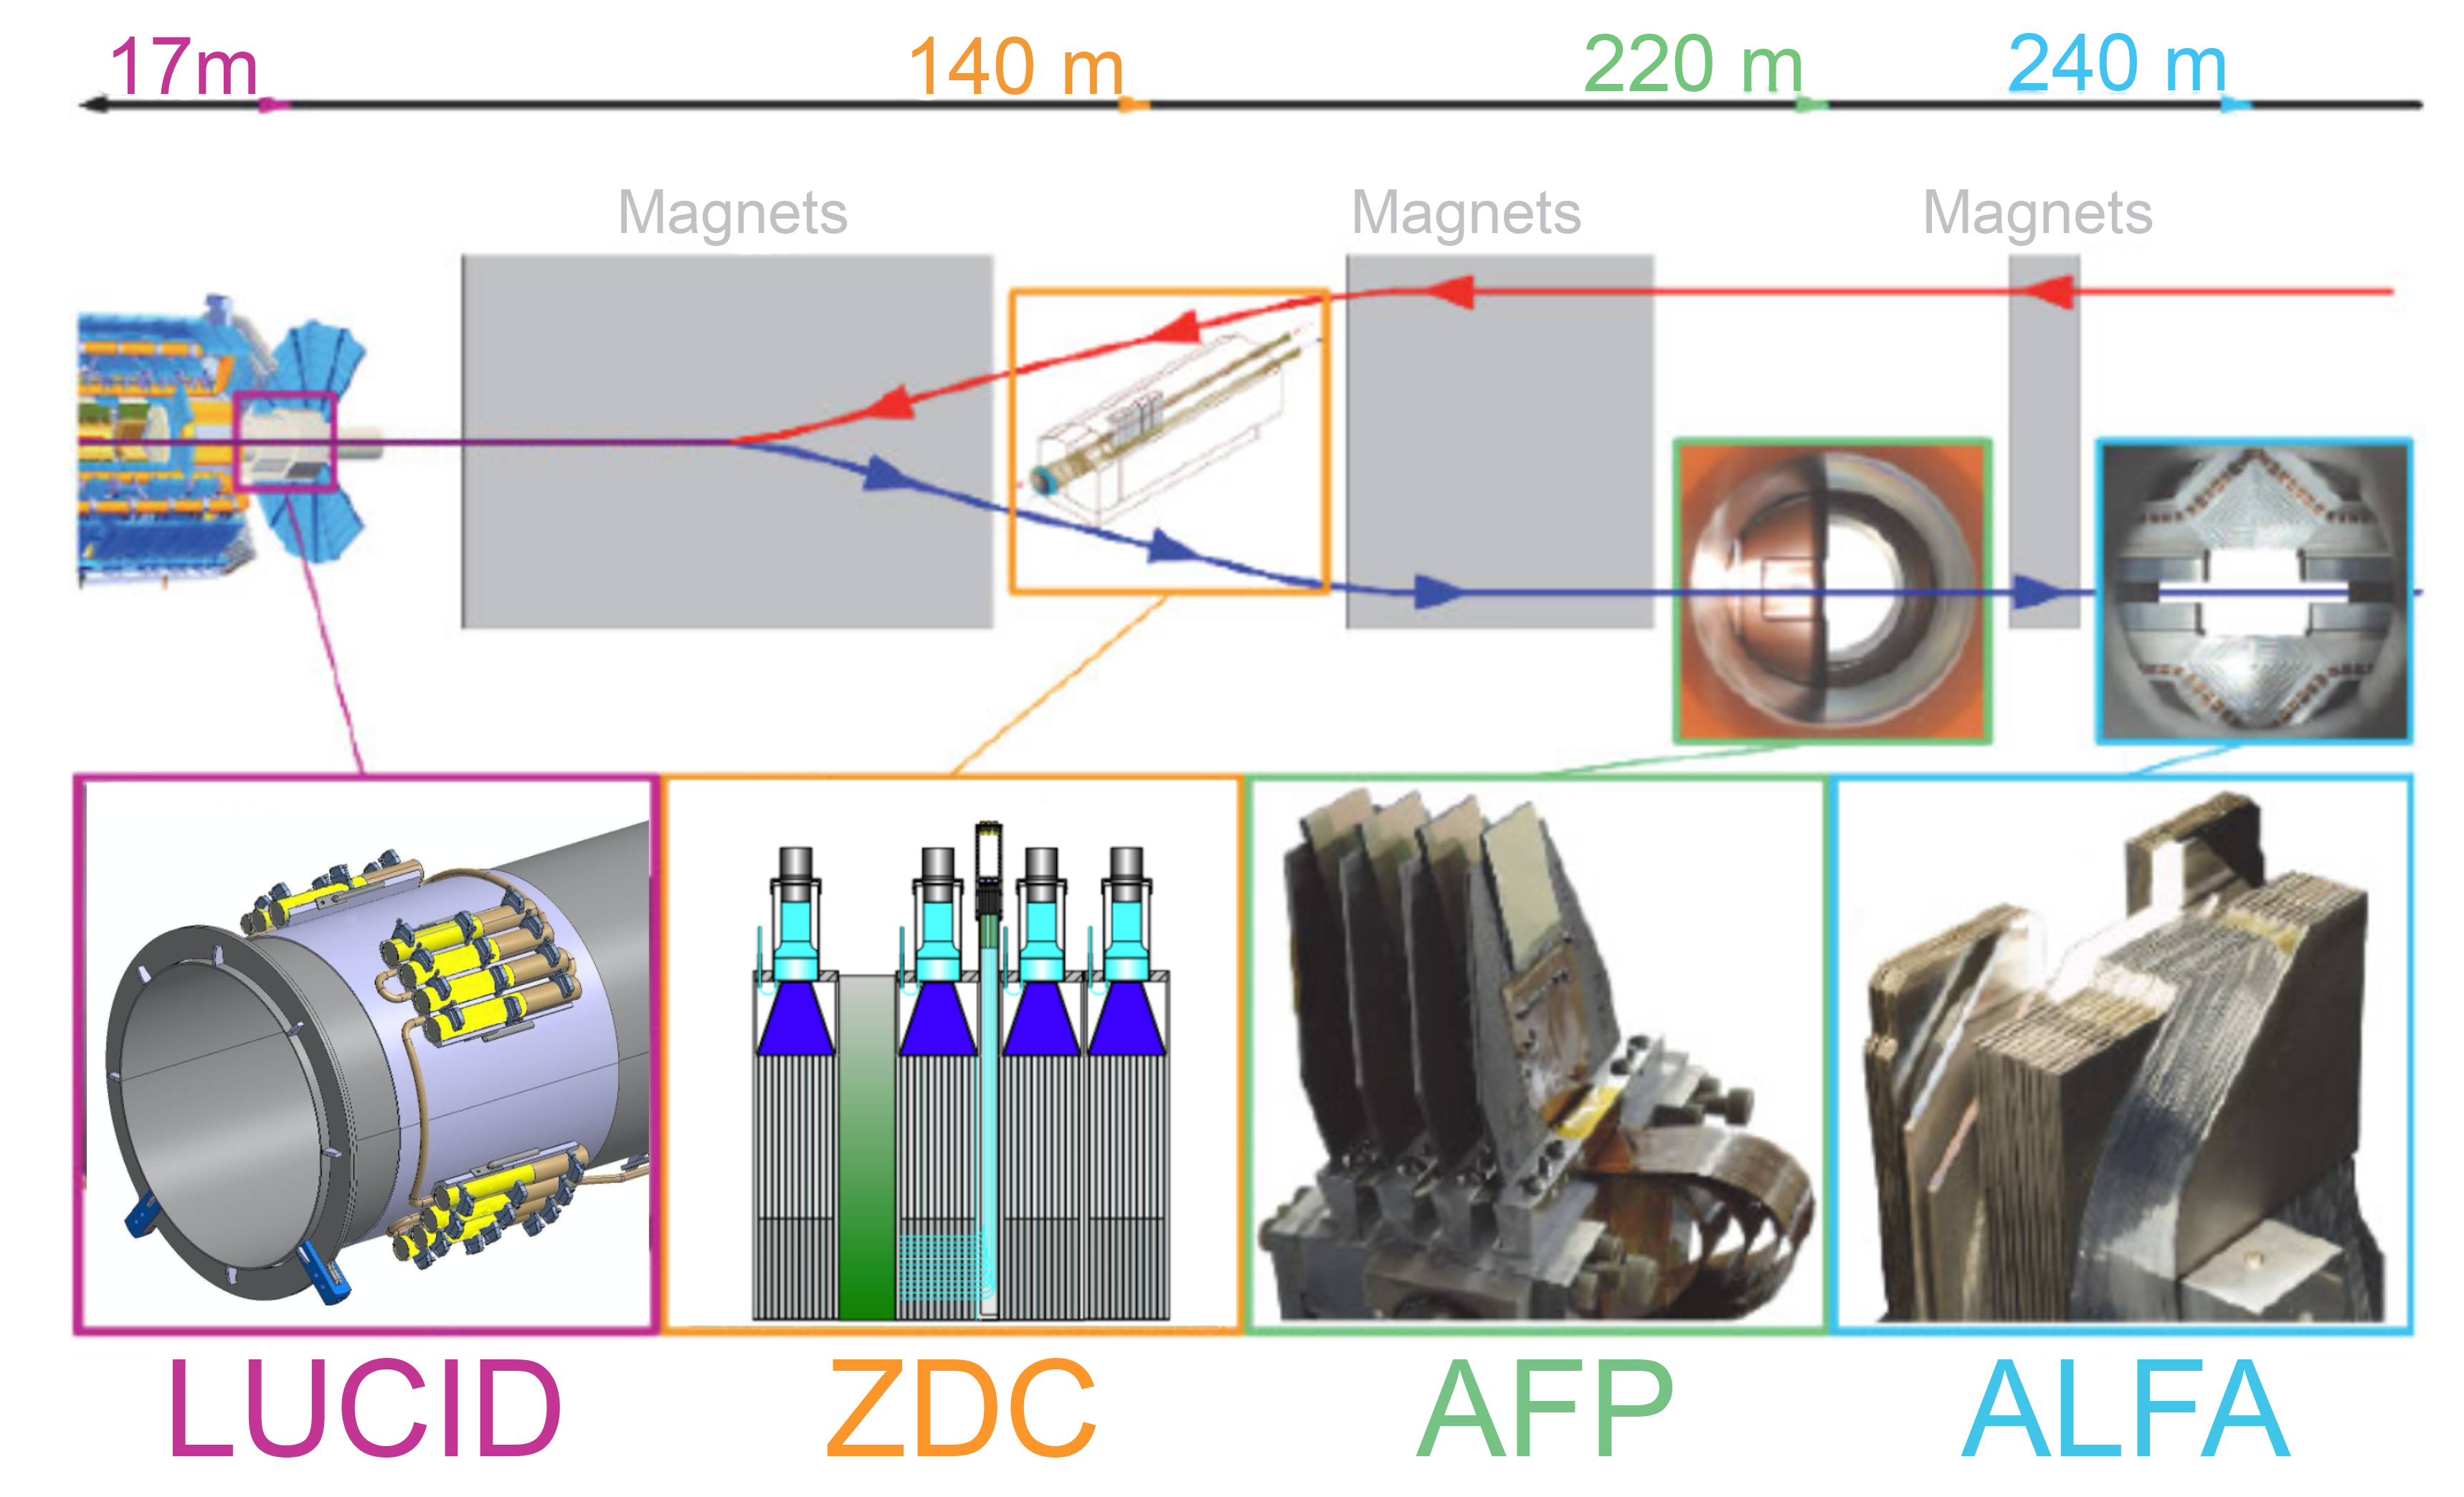
\includegraphics[width=1.0\textwidth]{ATLAS-FD-run3.png}
            \caption{Layout of the forward detectors in the ATLAS experiment, taken from~\cite{GENR-2019-02}.}
            \label{fig:Forward_detectors}
        \end{figure}

        The LUminosity Cherenkov Integrating Detector (LUCID)~\cite{LUCID2} is located at a distance of $\pm17$ meters 
        from the IP. It is primarily designed to monitor the luminosity online and offline by detecting 
        inelastic proton-proton scattering events in the forward direction. LUCID employs Cherenkov tubes 
        filled with $C_4F_{10}$ gas, which emit light when traversed by charged particles produced in 
        collisions. This light is then detected by photomultiplier tubes (PMTs), allowing for precise 
        luminosity measurements.

        The Zero Degree Calorimeters (ZDC) are located at $\pm140$ meters from the IP, just beyond where 
        the common straight-section vacuum pipe splits into two separate beampipes. The ZDC modules 
        consist of alternating layers of tungsten plates and quartz rods, optimised for detecting neutral 
        particles at pseudorapidities \(|\eta| \geq 8.2\). The ZDCs play a crucial role in determining the 
        centrality of heavy-ion collisions, providing insights into the collision geometry and the energy 
        deposition of forward-going neutrons and photons.

        The Absolute Luminosity for ATLAS (ALFA) Roman Pot detector consists of four stations positioned at $\pm240$
        meters from the IP. Each station includes two scintillating fibre trackers housed in Roman pots, 
        which can approach the LHC beam as close as 1 mm. ALFA is used in dedicated low-luminosity and 
        high-\(\beta^*\) runs to measure the total cross-section for proton-proton interactions through 
        elastic scattering and diffraction studies. In preparation of Run 3, 
        several upgrades were made to ALFA. The aged readout electronics and scintillating
        fibres were replaced, and additional shielding walls were installed to reduce radiation exposure
        and extend the operational lifespan of the detectors. The Roman Pot movement system was refurbished,
        and firmware updates were implemented for the central trigger processor input module to enhance 
        trigger and readout capabilities for ALFA-specific runs.

        The ATLAS Forward Proton (AFP) detector, part of the Phase I upgrade, is situated at $\pm205$ meters 
        (near stations) and $\pm217$ meters (far stations) from the IP. Each station contains a silicon 
        tracker (SiT) similar to the Insertable B-Layer (IBL) and a Time-of-Flight (ToF) detector. The 
        SiT provides precise measurements of the proton trajectories, while the ToF detector measures 
        the time difference between protons reaching the detectors, achieving vertex resolution of 3 to 5 mm.

        The AFP detector underwent several upgrades during LS2 to prepare for Run 3. These upgrades included:
        \begin{itemize}
            \item replacement of radiation-damaged silicon detectors with new 3D silicon pixel tracker modules.
            \item redesign of the ToF detector to prevent corona discharge issues in vacuum.
            \item updates to the trigger and readout electronics to improve timing resolution and data acquisition efficiency.
        \end{itemize}

        \begin{figure}[htbp]
            \centering
            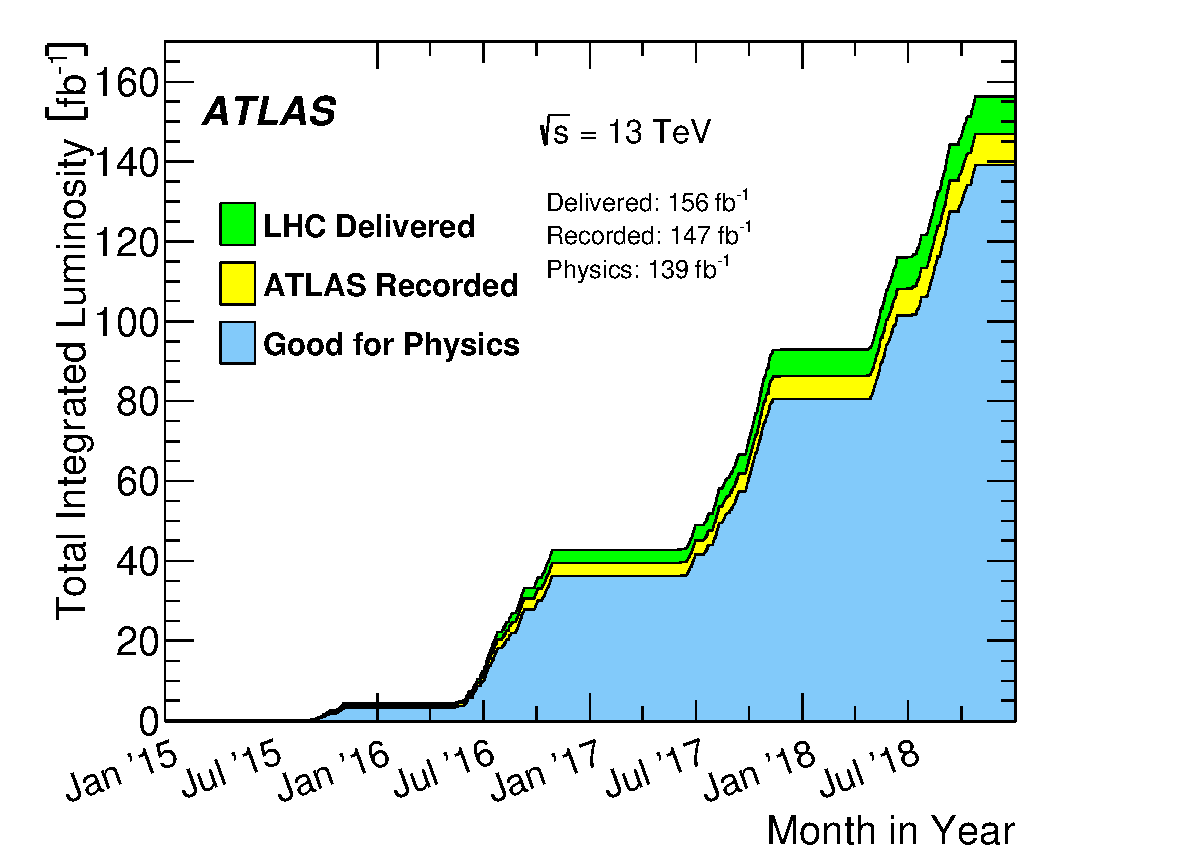
\includegraphics[width=0.5\textwidth]{total_lumi_run2.pdf}
            \caption{
                Cumulative integrated luminosity delivered to and recorded by ATLAS between 2015 and 2018 during stable beam pp collision data-taking at $\sqrt{s}=13$ TeV. This figure is taken from~\cite{DAPR-2018-01}.
            }
            \label{fig:run2lumi}
        \end{figure}

    \subsection{TDAQ System}
        The Trigger and Data Acquisition (TDAQ)~\cite{ATLAS-TDR-16} system of the ATLAS detector is a 
        sophisticated infrastructure designed to manage the immense amount of data generated by particle 
        collisions at the LHC. Its primary function is to select and record the most interesting 
        collision events for detailed analysis, thereby enabling the identification of rare physics 
        phenomena. A schematic of the ATLAS TDAQ system is shown in Figure~\ref{fig:TDAQ_schematic}.
        \begin{figure}[htbp]
            \centering
            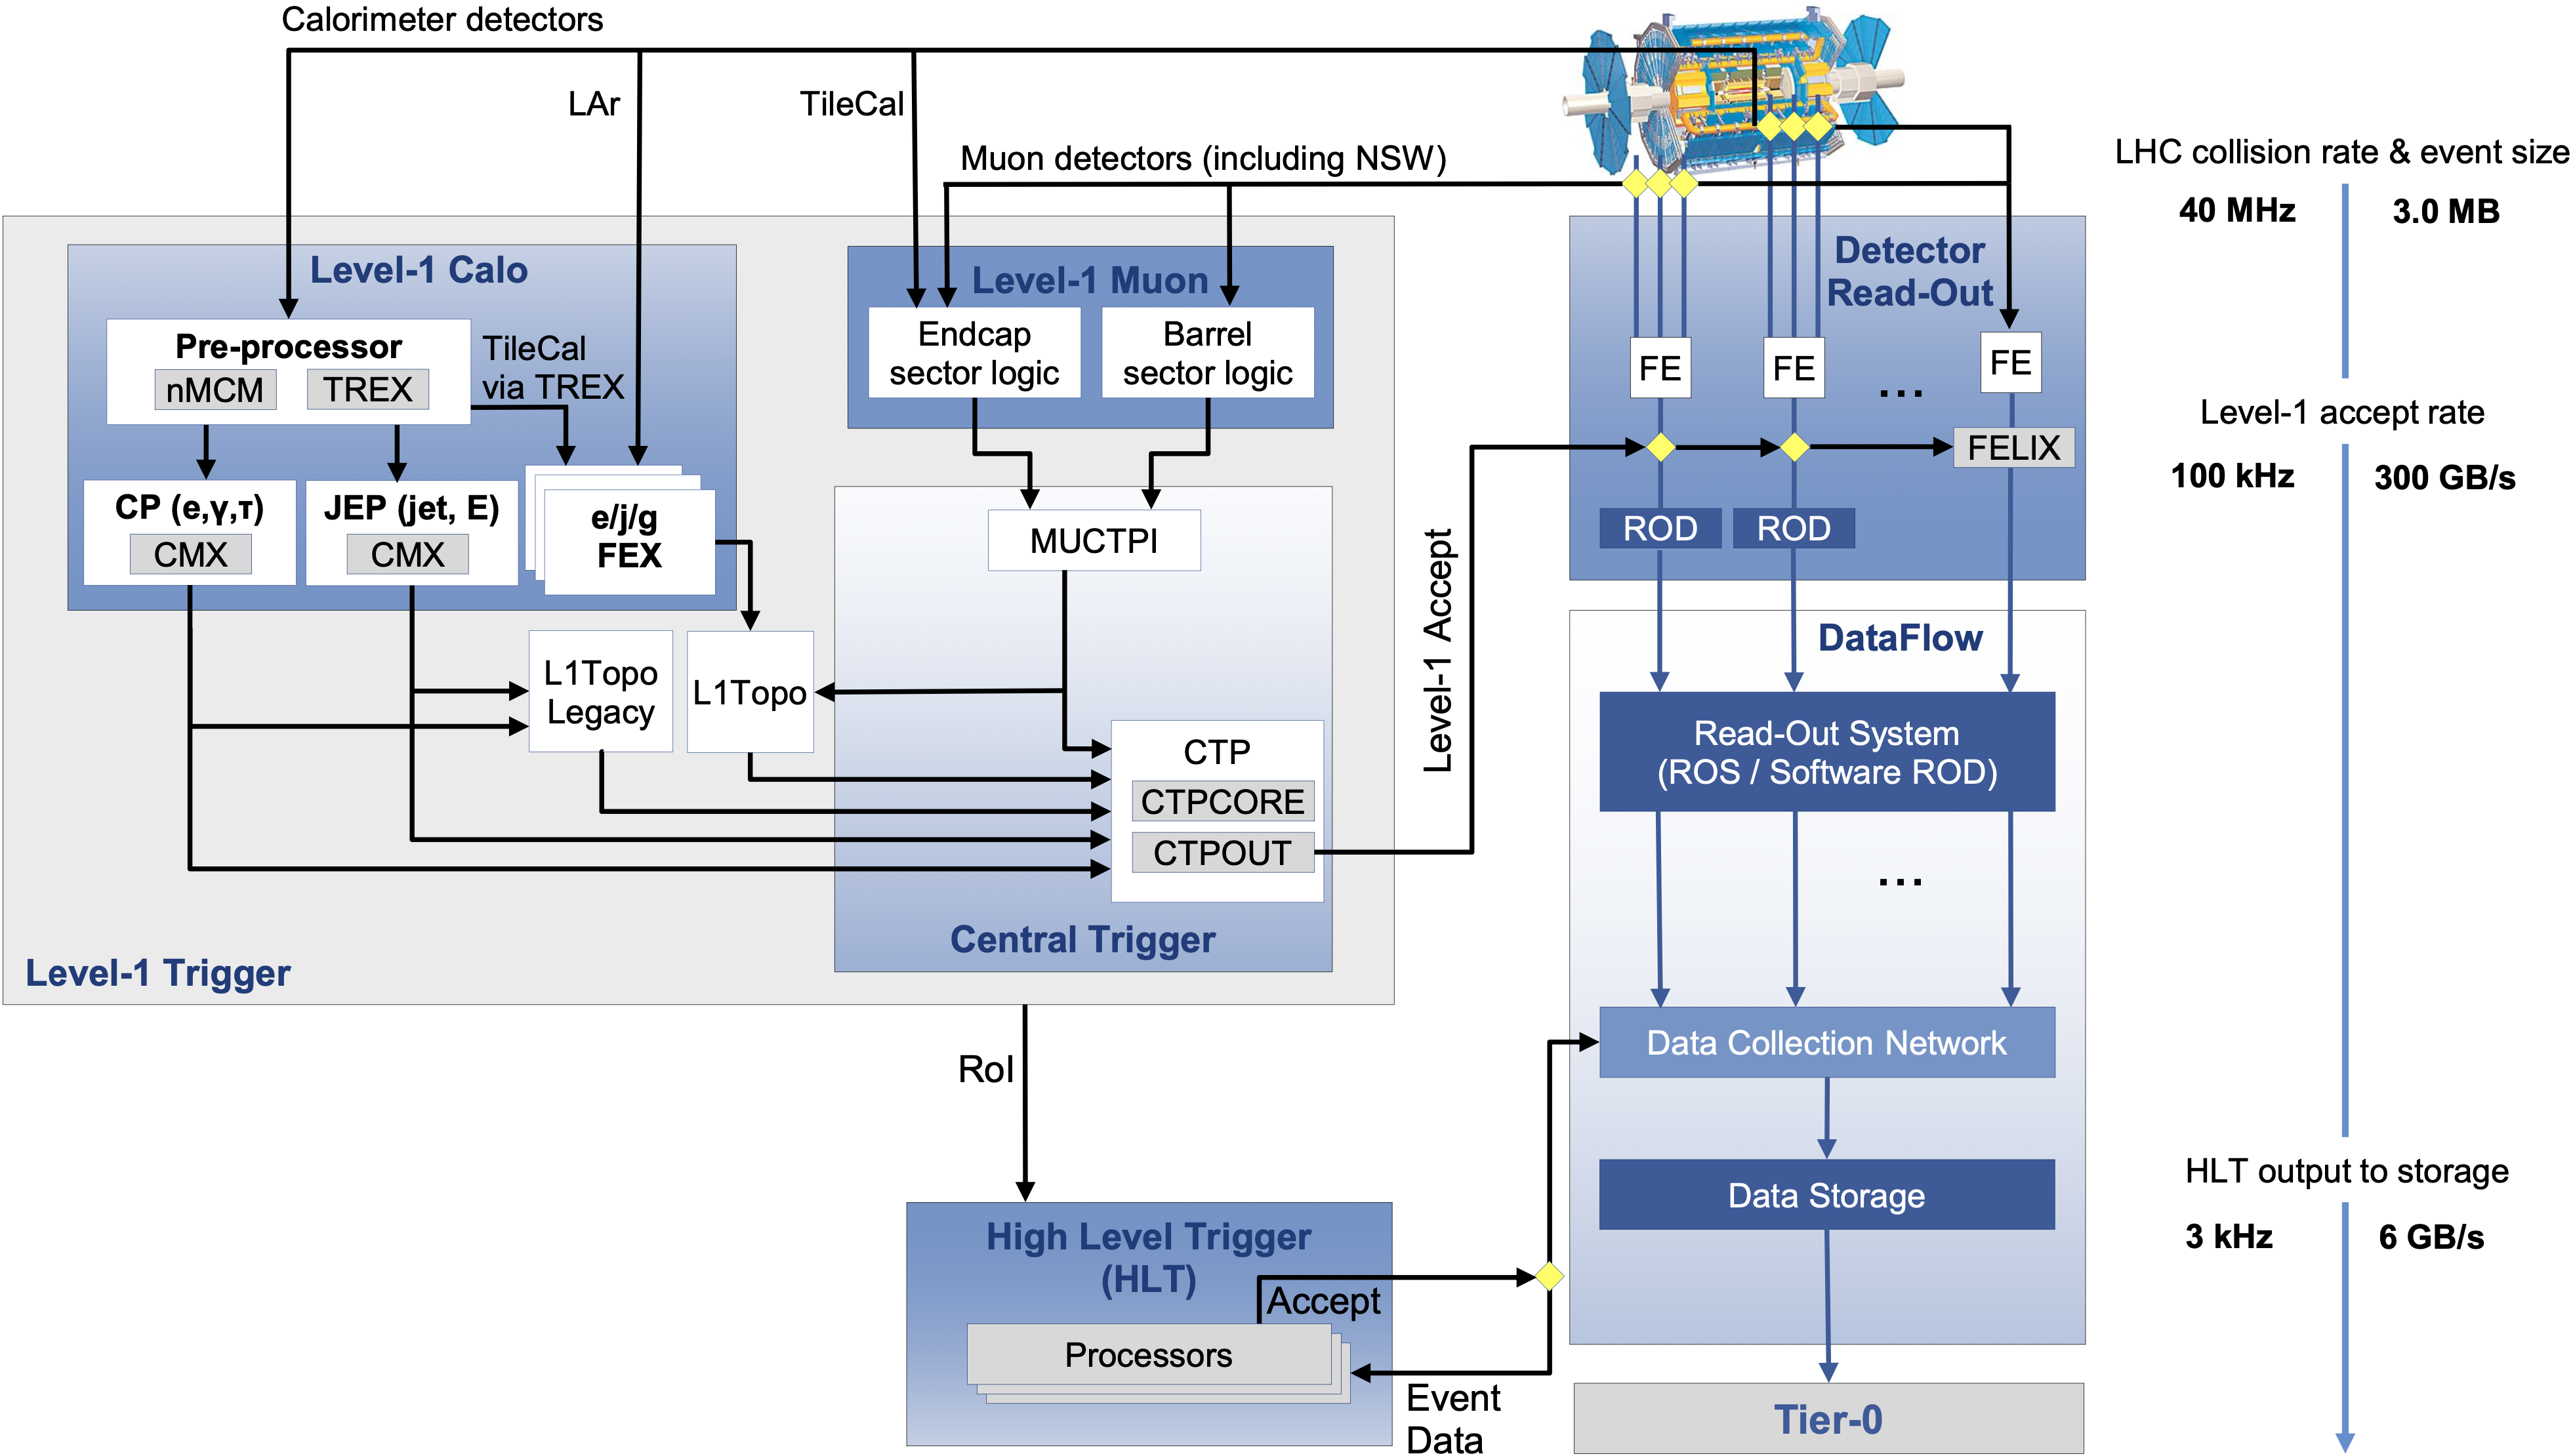
\includegraphics[width=1.0\textwidth]{ATLAS-TDAQ-run3.png}
            \caption{Schematic of the ATLAS Trigger and Data Acquisition (TDAQ) system, taken from~\cite{GENR-2019-02}.}
            \label{fig:TDAQ_schematic}
        \end{figure}
        The ATLAS TDAQ system employs a multi-tiered architecture that comprises the Level-1 (L1) Trigger, 
        the High-Level Trigger (HLT), and the Data Acquisition (DAQ) system. This design allows for efficient 
        and rapid data processing, ensuring that only the most relevant events are stored for further analysis. 

        The L1 Trigger is the first stage in the event-selection process. It operates directly on the raw data 
        from the detector, using custom-built hardware to analyse data with reduced granularity. The L1 Trigger 
        must make decisions within a strict latency of 2.5 microseconds to reduce the event rate from the 40 MHz 
        bunch crossing rate of the LHC to a maximum of 100 kHz. The L1 Trigger comprises the L1 calorimeter 
        triggers and the L1 muon triggers. Both subsystems generate Region of Interest (RoI) signals that guide 
        the HLT in its more detailed analysis.
        The HLT is a software-based system implemented on commercial processors. It performs detailed event 
        reconstruction using the full detector data, significantly refining the initial L1 selection. 
        The HLT reduces the event rate from the L1's 100 kHz to about 3 kHz for storage. Guided by RoIs from 
        the L1 Trigger, the HLT performs localised and full-event reconstruction. For Run 3, the HLT uses the 
        AthenaMT software framework, which allows for parallel processing and more efficient resource use. 
        Sophisticated algorithms, including those for track reconstruction and particle identification, 
        enhance the precision and efficiency of event-selection.
        The DAQ system is responsible for managing data flow from the detector front-end electronics to permanent 
        storage. It ensures that data from accepted events are properly formatted, transported, and recorded.
        Key components of the DAQ system include:
        \begin{itemize}
            \item Readout System (ROS): The ROS collects data from sub-detectors following an L1 accept and 
            buffers it for HLT processing.
            \item Data Collection Network: This high-bandwidth network facilitates data transfer from the 
            ROS to the HLT processing farm.
            \item Data Storage: Events accepted by the HLT are transferred to permanent storage for offline 
            analysis. The system is designed to handle an average output of 3 kHz, corresponding to a data 
            throughput of 6 GB/s.
        \end{itemize}
        Several upgrades have been implemented in the TDAQ system for Run 3~\cite{ATLAS-TDR-23} to cope with higher luminosities 
        and increased data rates. Upgraded L1 Trigger electronics and algorithms provide finer granularity 
        and improved selectivity, allowing for better background rejection and more efficient event-selection.
        Level-2 (L2) and event filter (EF) systems used in the previous runs have been integrated into a 
        single HLT framework, streamlining the data processing pipeline and improving resource utilisation.
        The computational resources of the TDAQ systems have been expanded to handle the increased data 
        volume and complexity, ensuring that event reconstruction and selection can be performed with high 
        efficiency. Enhancements in data management and storage infrastructure ensure that the system can 
        handle the increased data volume and maintain data integrity.
\section{Object reconstruction and identification in ATLAS} 
    \subsection{Reconstruction and identification of electrons and photons} 
        \subsubsection{Egamma reconstruction}
            The reconstruction of electrons and photons (collectively known as Egamma)~\cite{EGAM-2018-01, EGAM-2021-01} in the ATLAS detector is a multi-step process that 
            involves the collection of energy deposits in the electromagnetic calorimeter and matching these deposits to tracks reconstructed 
            in the ID. The energy of electron and photon candidates is reconstructed by clustering the energy deposits in the cells of the 
            EM calorimeter. The algorithm used is optimised to handle the different shower shapes and energy distributions of electrons and 
            photons. Superclusters are formed by combining clusters from the presampler and multiple calorimeter layers, using a 
            boosted-decision-tree (BDT) regression algorithm to optimise the energy measurement. This approach accounts for variations 
            in the particle's incident angle and position within the detector. For electrons, the energy clusters are matched to tracks 
            reconstructed in the ID. The matching is based on the consistency between the cluster position and the extrapolated track position 
            at the calorimeter. A combination of criteria, including the ratio of the track momentum to the cluster energy (E/p) and the shower 
            shape, is used to enhance the identification efficiency and purity. This matching process helps distinguish electrons from hadronic 
            background and photon conversions.
            Photons are identified through their characteristic energy deposits in the EM calorimeter. Unconverted photons, which do not 
            interact in the ID, are identified purely based on the calorimeter information. Converted photons, which produce an electron-positron 
            pair in the ID, require reconstruction of the conversion vertex and matching of the resulting tracks to the calorimeter clusters. 
            The photon identification criteria involve isolation requirements and shower shape variables to reduce background from neutral hadrons and jets.
            \begin{figure}[htbp]
                \centering
                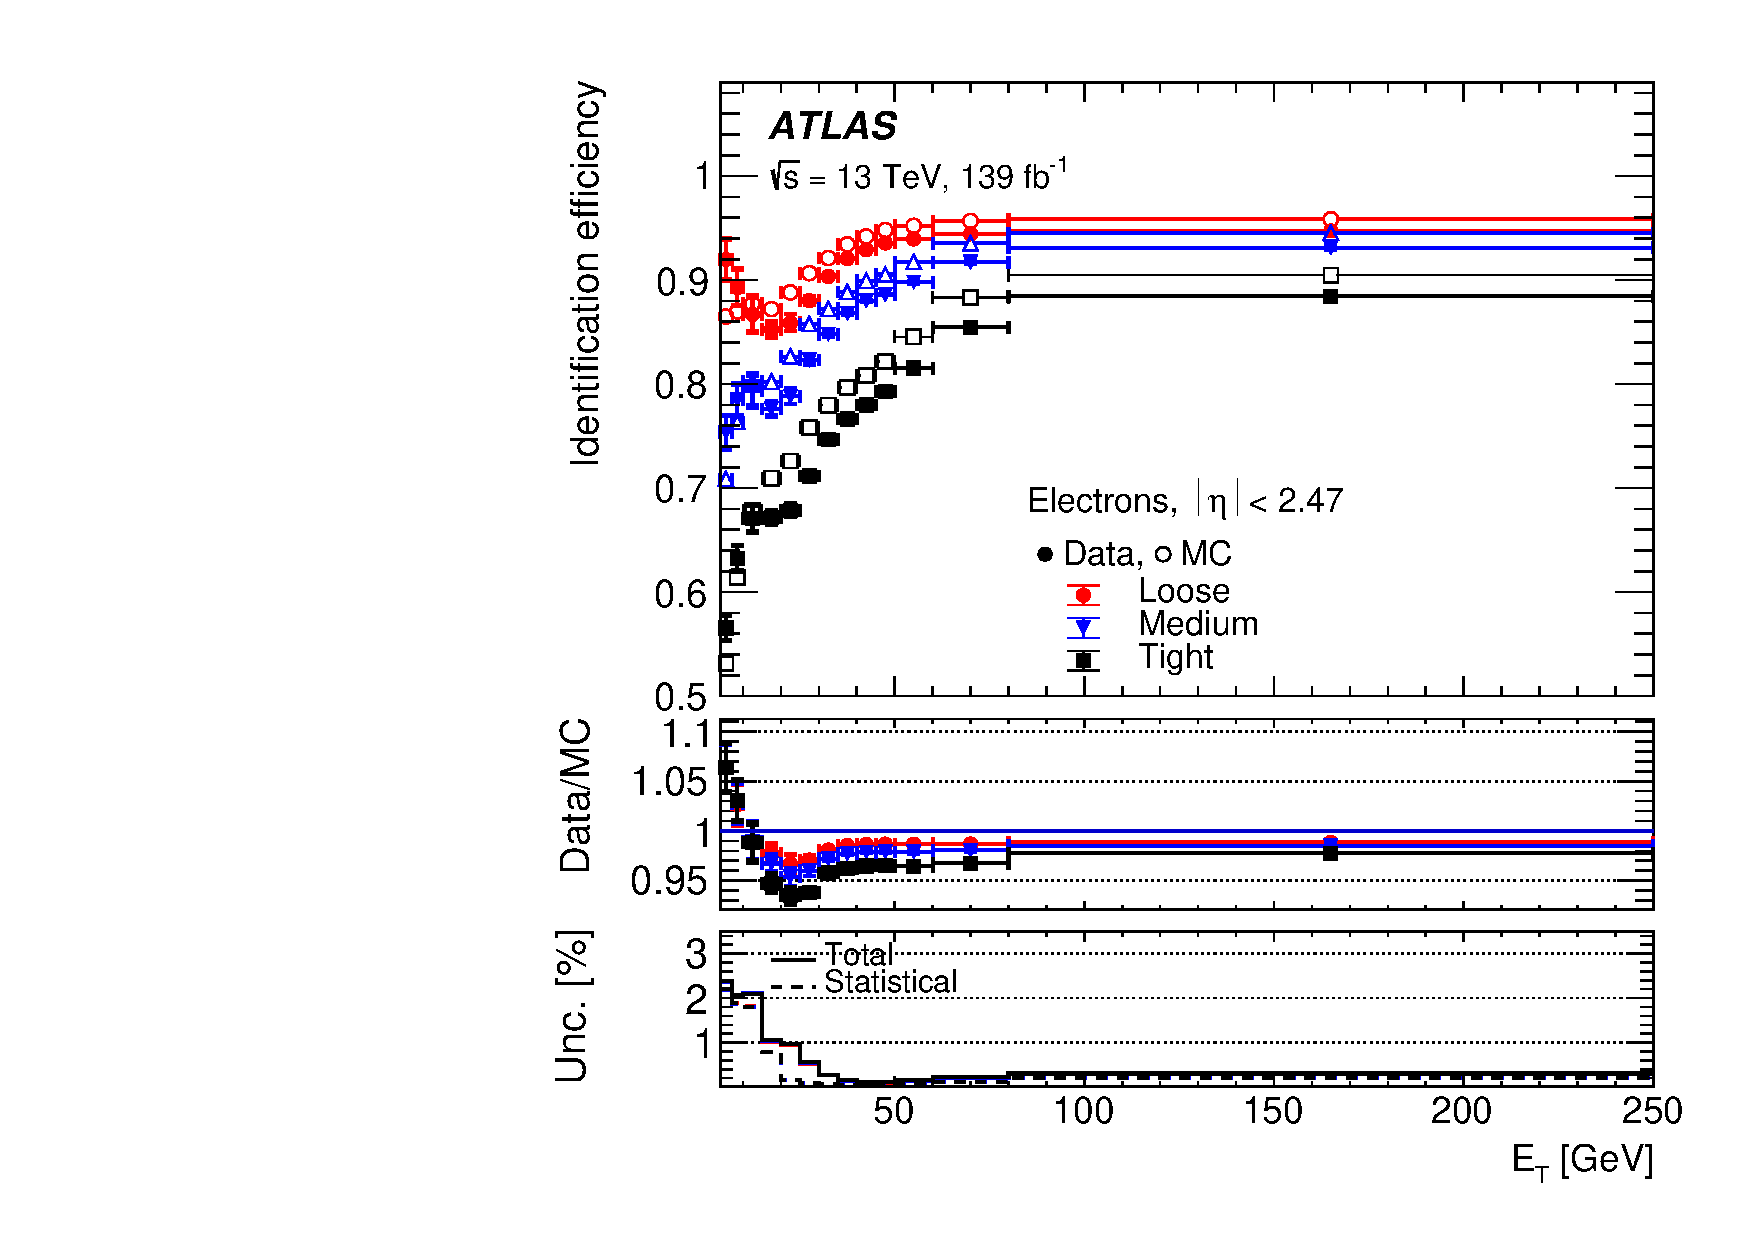
\includegraphics[width=0.5\textwidth]{elec_effi_pt.pdf}
                \caption{
                    Identification efficiencies of electrons from $Z\rightarrow ee$ decays as a function of the electron's transverse momentum for the different identification working points. This figure is taken from~\cite{EGAM-2021-01}.
                }
                \label{fig:elec_effi}
            \end{figure}
        \subsubsection{Egamma calibration}
            The calibration of electron and photon energies~\cite{EGAM-2021-02} is crucial for achieving precise measurements required for ATLAS physics analyses. 
            The calibration procedure involves several steps to correct for detector response variations and ensure consistency between data and simulation.
            The EM calorimeter is segmented into longitudinal layers, each of which responds differently to incident particles. The first step in the 
            calibration process involves correcting the energy response of each layer to account for these variations. This is achieved using detailed 
            simulations and data-driven techniques to ensure accurate energy measurements across the detector. A simulation-based BDT regression 
            algorithm is used to combine the energy deposits from different calorimeter layers and the presampler. This algorithm is trained to 
            optimise the energy measurement separately for electrons, converted photons, and unconverted photons, considering the particle's position 
            and angle of incidence. The simulation-based calibration is applied uniformly to data and simulated events. Several corrections are applied 
            to account for residual differences between data and simulation. These include adjustments for non-uniformities in the detector response, 
            variations in the high-voltage settings, and corrections for biases introduced by the liquid-argon calorimeter electronics. The stability 
            of the calorimeter response over time and across different detector regions is also monitored and corrected as necessary. The final calibration 
            step involves adjusting the global energy scale using samples of $Z \rightarrow ee$ events. The peak of the reconstructed Z boson mass is 
            aligned between data and simulation to ensure consistency. This step also includes smearing the energy resolution in the simulation to match 
            that observed in the data, thereby correcting for any discrepancies in the detector's energy response. Photon-specific calibration steps are 
            needed to account for differences in the lateral development of electron and photon showers. Corrections are derived from studies of out-of-cluster 
            energy leakage and the modelling of photon reconstruction efficiencies. These corrections ensure that the energy measurements for photons are 
            as precise as those for electrons.

            The calibrated energy measurements are validated using independent data samples, such as $J/\psi \rightarrow ee$ and $Z \rightarrow ll\gamma$ events. 
            The systematic uncertainties associated with the calibration are thoroughly evaluated, accounting for factors such as the passive material model, 
            the electronic noise, and the pile-up conditions. 

        \subsubsection{Neural Network (NN) based electron identification}
            Two significant developments in this area are the use of Deep Neural Networks (DNNs)~\cite{ATL-PHYS-PUB-2022-022} and Convolutional Neural Networks (CNNs)~\cite{ATL-DAPR-PUB-2023-001}
            for electron identification.
            The DNN-based electron identification algorithm leverages high-level discriminating variables derived from the reconstructed electron track and calorimeter 
            energy deposits. The DNN algorithm enhances electron identification performance by optimising the correlations between input features, which are often 
            neglected in traditional likelihood-based approaches. By performing multinomial classification, the DNN can categorise electron backgrounds into several 
            classes, such as electrons from heavy-flavour decays or light-flavour hadrons, enabling targeted background rejection. This approach has demonstrated 
            a significant increase in combined background rejection, with improvements ranging from 1.7 to 5.5 times compared to previous methods for a fixed signal efficiency.
            The CNN-based algorithm further refines electron identification by processing low-level detector information, such as calorimeter cell energy deposits, 
            which are treated as images. The CNN architecture is specialised in image recognition, allowing it to effectively analyse the spatial patterns of energy 
            deposits. This algorithm integrates high-level features used in DNNs and additional tracks matched to electron candidates, which enhances its performance. 
            The CNN has shown remarkable improvements in background rejection, particularly for light-flavour hadrons and electrons from photon conversions. For 
            instance, it achieves background rejection factors up to five times better than the likelihood-based method for charged hadrons faking electron signatures. 
            The CNN's ability to output a vector of probabilities for different electron classes further enhances its flexibility and accuracy in various analyses.

            These advancements are crucial for enhancing the precision of physics analyses conducted at the ATLAS experiment, particularly 
            those involving multiple leptons or requiring stringent electron background rejection. In the future, these neural network-based approaches will 
            continue to evolve, potentially incorporating real data for training to overcome simulation biases and improve generalisation to actual collision 
            events. Adversarial training techniques might also be employed to mitigate differences between simulated and real data, further refining the performance 
            of electron identification algorithms in ATLAS.

    \subsection{Jet reconstruction}
        Jets are collimated streams of particles that result from the hadronisation of quarks and 
        gluons produced in high-energy processes. As a direct consequence of the running of the 
        strong coupling constant, and the QCD colour confinement, when quarks and gluons are produced in a collision, 
        they cannot exist freely. Instead, they fragment into a cascade of hadrons, predominantly 
        pions and kaons, which cluster together to form jets. The ATLAS experiment employs sophisticated 
        jet reconstruction techniques to accurately identify and measure jets. 
        The reconstruction processes have evolved to utilise both calorimetric and tracking information, 
        enhancing the precision and robustness of jet measurements. The two primary methods are based on calorimeter 
        information and the particle flow (PFlow) algorithm~\cite{PERF-2015-09}, both of which use the anti-kt 
        algorithm~\cite{Cacciari:2008gp} with a radius parameter \( R = 0.4 \). A larger radius parameter 
        (\( R = 1.0 \)) is used for large-radius jets optimised for boosted object identification~\cite{JETM-2023-02}.

        \subsubsection{Calorimeter-based jet reconstruction}
            In the calorimeter-based method, jets are reconstructed using three-dimensional topological clusters 
            (topo-clusters)~\cite{PERF-2014-07, JETM-2023-01} of calorimeter cells. These cells are grouped together based on their energy depositions 
            and spatial proximity using a nearest-neighbour algorithm. The energy of these clusters is initially 
            calibrated to the electromagnetic (EM) energy scale, which is suitable for measuring energy depositions from 
            electromagnetic showers. Only positive-energy topo-clusters are used as inputs to the jet reconstruction. 
            An origin correction is applied to each topo-cluster to account for the position of the primary vertex, 
            ensuring that the jet's energy and direction are accurately determined with respect to the event's primary vertex.

            EMtopo jets, reconstructed using origin-corrected EM scale topo-clusters, 
            were the primary jet definition used in ATLAS physics analyses conducted in Run 2. 
            These jets exhibited robust energy scale and resolution characteristics 
            across a wide kinematic range and were independent of other reconstruction algorithms such as tracking at the 
            jet-building stage~\cite{JETM-2018-05}.

        \subsubsection{Particle Flow (PFlow) algorithm}
            The particle flow algorithm aims to improve jet reconstruction by combining measurements from both 
            the tracking and calorimeter systems~\cite{JETM-2018-05}. This approach reconstructs individual particles by replacing 
            the energy deposited in the calorimeter by charged particles with the momenta of tracks matched to 
            those deposits. The PFlow algorithm uses the following steps:
            \begin{itemize}
                \item Track Selection: Tracks are selected based on quality criteria, such as a transverse momentum 
                (\( p_T \)) threshold of 500 MeV and a distance of closest approach to the primary vertex along the 
                z-axis less than 2 mm. This selection helps to suppress pile-up contributions by rejecting tracks not 
                associated with the primary vertex.
                \item Energy Subtraction: The energy deposited by charged particles in the calorimeter is subtracted, 
                and the corresponding track momenta are used instead. This subtraction is carefully managed to avoid 
                removing energy deposited by other particles.
                \item Topo-Cluster Adjustment: The \( \eta \) and \( \phi \) coordinates of topo-clusters are recomputed
                with respect to the primary vertex position. This adjustment ensures that the reconstructed jets are aligned 
                correctly with the hard-scatter interaction.
            \end{itemize}
            PFlow jets, formed from these combined signals, exhibit improved energy and angular resolution, reconstruction 
            efficiency, and stability against pile-up effects compared to jets reconstructed using calorimeter information alone.

        \subsubsection{Jet calibration and performance}
            Calibration of the reconstructed jets involves several steps to ensure their energy scale matches the particle level~\cite{JETM-2018-05, JETM-2022-01}. 
            Firstly, pile-up corrections remove excess energy due to additional proton-proton interactions within the same or nearby 
            bunch crossings. They consist of a jet area-based correction and a residual correction derived from Monte Carlo (MC) simulations.
            The second step is the absolute energy scale calibration, this step corrects the jet energy and direction to match those of 
            particle-level truth jets. It is typically derived from dijet MC events. Then, the global sequential calibration process 
            reduces the dependence of the reconstructed jet response on tracking, calorimeter, and muon chamber information, further 
            refining the energy resolution and reducing systematic uncertainties. Finally, the in situ calibration corrects any remaining
            differences between data and MC simulation using well-measured reference objects such as photons, Z bosons, and calibrated jets.
            The final step is applied to data only.
            These methods ensure that ATLAS can precisely reconstruct and measure jets.
            \begin{figure}[htbp]
                \centering
                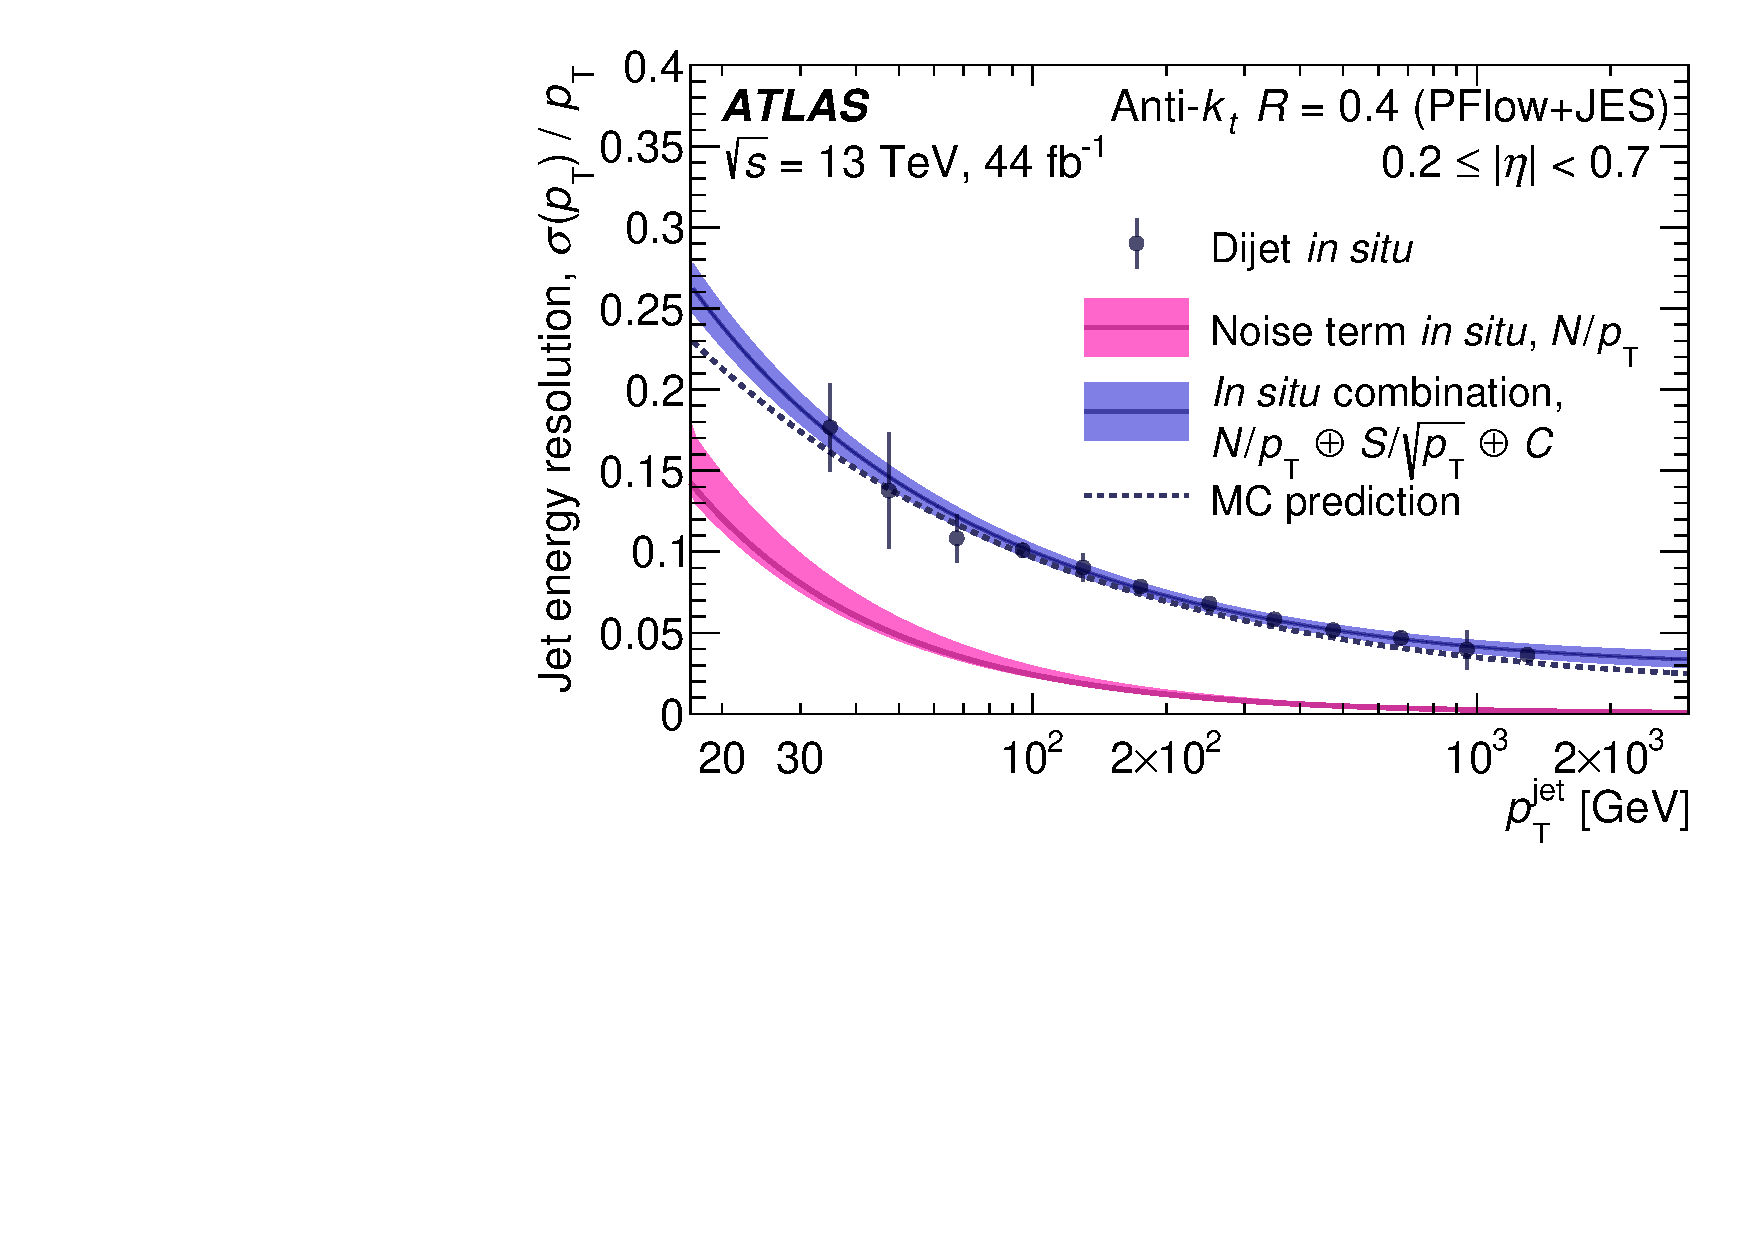
\includegraphics[width=0.495\textwidth]{jet_reso.pdf}
                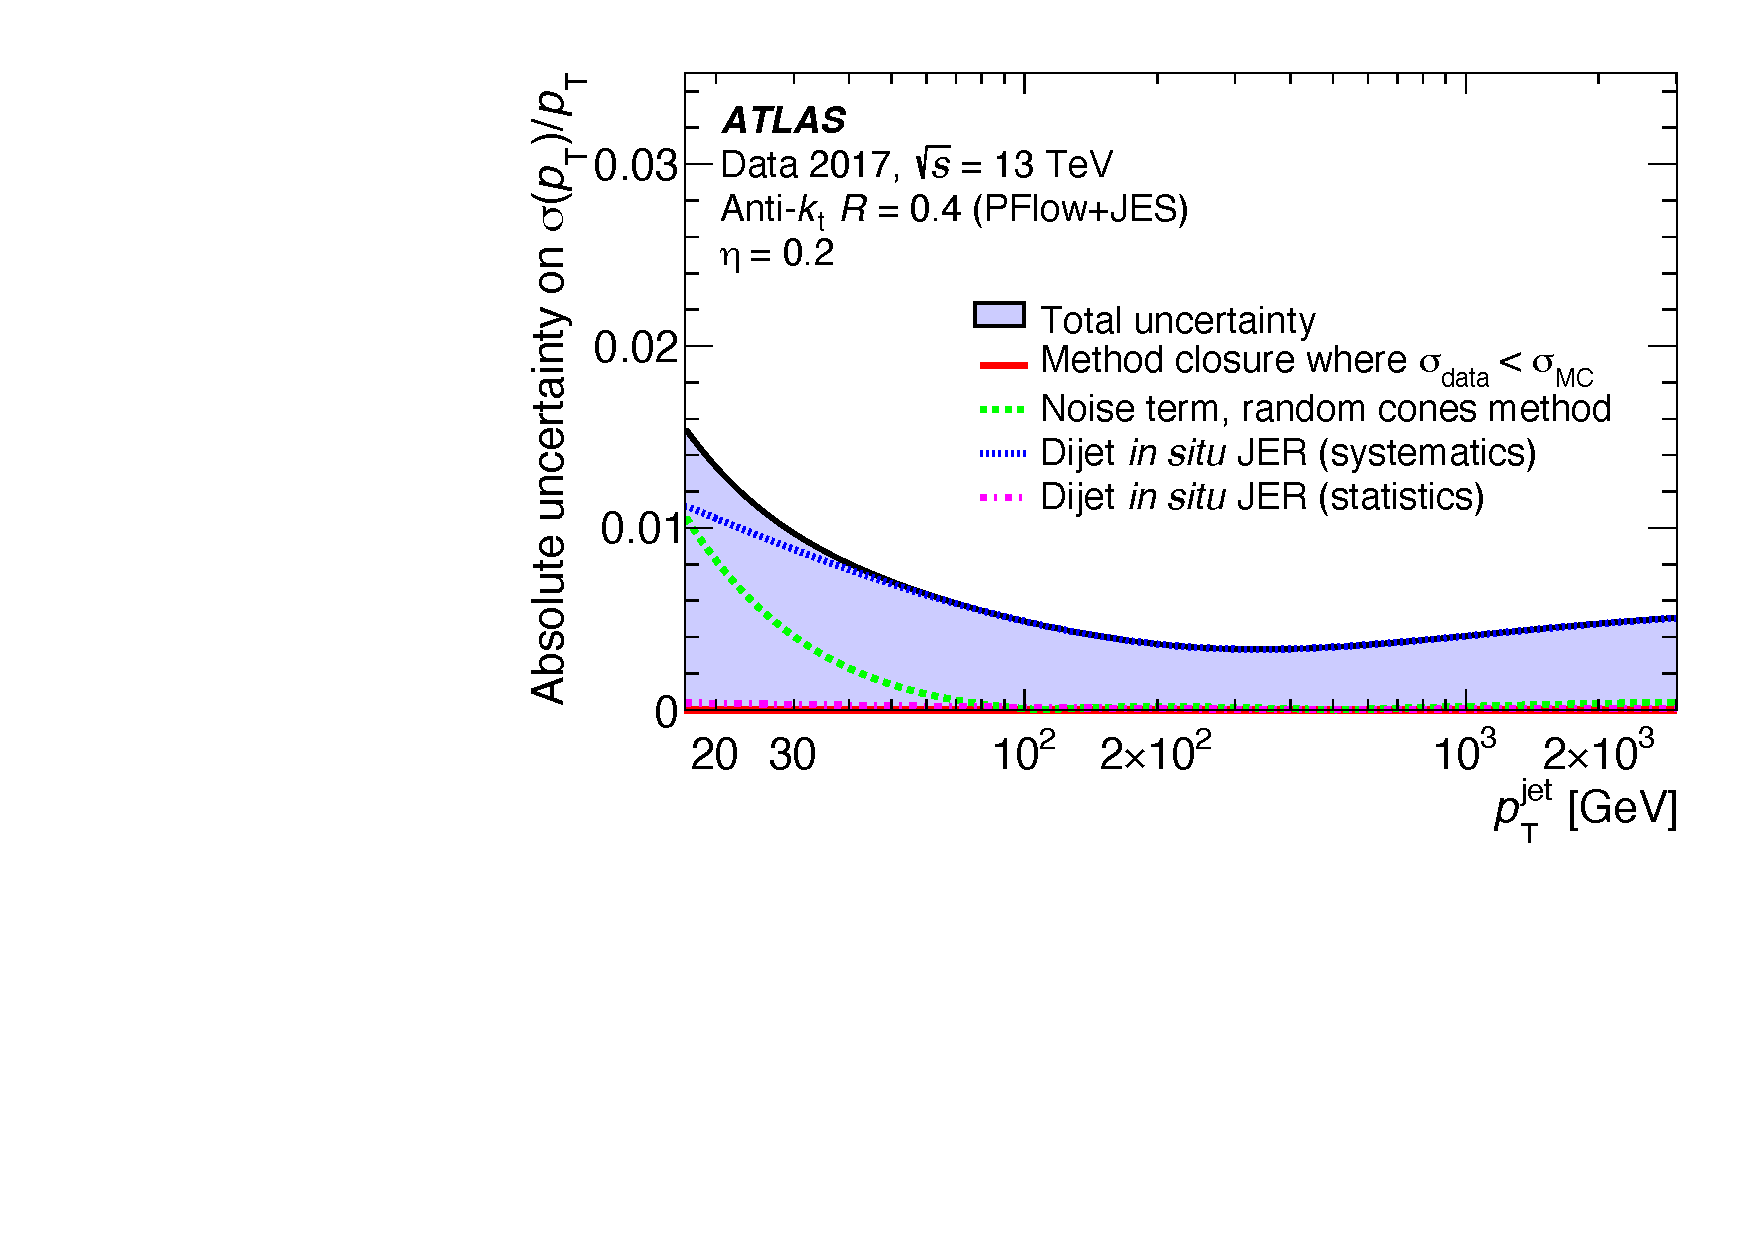
\includegraphics[width=0.495\textwidth]{jet_uncert.pdf}
                \caption{
                    (left) The relative jet energy resolution as a function of $\pt$ for fully calibrated PFlow+JES jets. 
                    The error bars on points indicate the total uncertainties on the derivation of the relative resolution in dijet events, 
                    adding in quadrature statistical and systematic components. 
                    The expectation from Monte Carlo simulation is compared with the relative resolution as evaluated in data through the combination of the dijet balance and random cone techniques. 
                    (right) Absolute uncertainty on the relative jet energy resolution as a function of jet $\pt$. 
                    Uncertainties from the two in situ measurements and from the data/MC simulation difference are shown separately.
                    These figures are taken from~\cite{JETM-2018-05}.
                }
                \label{fig:jet_reso}
            \end{figure}

        \subsubsection{Large-radius jets}
            Large-radius jets are specifically optimised to identify highly boosted topologies, particularly those involving boosted objects 
            such as \(W\), \(Z\), and Higgs bosons, as well as top quarks~\cite{JETM-2018-03}. These jets are typically reconstructed using the anti-\(k_t\) 
            algorithm with a large radius parameter (\(R = 1.0\)). The substantial radius allows the jet to capture more of the 
            radiation and decay products from highly boosted massive particles, thus providing a clearer insight into their substructure.
            In Run 2 and Run 3, the unified flow objects (UFOs)~\cite{JETM-2018-02,JETM-2018-06} have been developed to address the need for a jet input object that 
            combines desirable aspects of PFlow and Track-CaloClusters (TCC)~\cite{JETM-2018-02} reconstruction. This integration aims to further optimise 
            performance metrics, such as jet energy resolution and pile-up stability, across the full kinematic range.
            The UFO reconstruction process begins with the standard ATLAS PFlow algorithm. Charged PFlow objects (PFOs) matched 
            to pile-up vertices are removed, ensuring that only relevant tracks from the primary vertex are considered.
            The remaining PFOs are categorised into three category: neutral PFOs, charged PFOs used for subtracting energy from a topocluster,
            and charged PFOs in dense environments. In these dense environments, charged particles produced in regions is very high, 
            the detector may encounter challenges in isolating individual particle signals, and as a result, 
            no energy subtraction is performed for these PFOs.
            Jet-input-level pile-up mitigation algorithms, such as Constituent Subtraction (CS) and SoftKiller (SK)~\cite{ATLAS-CONF-2017-065}, 
            are applied to neutral PFOs to further reduce pile-up effects. A modified version of the TCC splitting algorithm is 
            then applied, using only tracks from the primary vertex to avoid pile-up instabilities. Tracks used for PFlow 
            subtraction are excluded from this step, as their contributions have already been subtracted.
            UFOs demonstrate improved tagging performance across both low and high \( p_T \) ranges, showing superiority over 
            TCC jets at high \( p_T \) and becoming comparable to PFlow jets at lower \( p_T \). Due to the inclusion of only 
            charged-particle tracks matched to the primary vertex, UFOs exhibit natural stability against pile-up, similar to 
            the PFlow algorithm. Additional stability is provided by input-level pile-up mitigation algorithms applied to neutral 
            particles. UFOs offer an improved jet mass resolution compared to existing large-\( R \) jet definitions, with up to a 
            45\% improvement at high \( p_T \) for signal jets. 
            However, the calibration process for UFOs is more complex due to the need to account for various factors such as the
            pile-up contribution and the energy scale of different components~\cite{JETM-2023-02}. 


    \subsection{Missing transverse energy (\MET) reconstruction}
        Missing transverse energy, also referred to as missing transverse momentum, serves as a proxy for the transverse momentum 
        carried by undetected particles, which can be indicative of phenomena such as neutrino production within the SM or 
        potential new physics scenarios like dark matter.
        The reconstruction of \MET~\cite{JETM-2020-03} involves the combination of multiple detector inputs, including calibrated electrons, muons, photons, hadronically decaying 
        \(\tau\)-leptons, hadronic jets, and soft activity from remaining tracks. This process is inherently complex due to the need to avoid double-counting 
        of momentum and to accurately represent the event's transverse momentum balance.
        \subsubsection{\MET reconstruction}
            The reconstruction process of \MET in ATLAS is divided into two main components:
            \begin{itemize}
                \item Hard Term (\(p_T^{\text{hard}}\)): This includes signals from well-reconstructed and calibrated hard objects such as electrons, 
                photons, \(\tau\)-leptons, muons, and jets. Each of these objects is carefully selected and calibrated to ensure accurate measurement.
                \item Soft Term (\(p_T^{\text{soft}}\)): This consists of contributions from tracks associated with the primary interaction vertex but not 
                associated with any hard object. The soft term helps capture the residual transverse momentum in the event that is not accounted for by the hard objects.
            \end{itemize}
            To form the \MET vector, these components are combined as follows:
            \[ 
            \vec{E}_T^{\text{miss}} = - \left( \sum \vec{E}_T^{\text{hard}} + \sum \vec{E}_T^{\text{soft}} \right)
            \]
            where the sums run over all selected hard objects and soft tracks, respectively.
            One of the key challenges in \MET reconstruction is avoiding double counting of detector signals. This is managed through a signal ambiguity resolution 
            procedure that ensures each detector signal contributes to only one hard object. The procedure priorities signals by a set of criteria, detailed in~\cite{olr:exact}
        \subsubsection{\MET calibration}
            ATLAS has defined several \MET working points, each with varying levels of stringency on jet selections to manage pile-up and other sources of fake 
            \MET. These working points range from loose to tenacious, with the latter offering the highest resilience to pile-up by applying more stringent 
            requirements on jets, particularly in the forward region of the detector.
            The performance of \MET reconstruction is evaluated using both real data and MC simulations. The key metrics for performance include 
            the resolution of \MET and its systematic uncertainties. The resolution is typically assessed in events with well-known kinematic properties, such 
            as \(Z \rightarrow \ell^+\ell^-\) decays, which provide a clean sample with no true \MET.
            The adoption of a particle flow algorithm, which combines calorimeter and tracking information, improves the resolution of jets. 
            This, in turn, facilitates dynamic \MET reconstruction that adapts based on the chosen hard objects in an analysis.
            Systematic uncertainties are thoroughly evaluated for both the hard and soft components of \MET. Recent studies have shown significant 
            reductions in scale and resolution uncertainties, thanks to improved calibration techniques and better handling of pile-up effects.
            \begin{figure}[htbp]
                \centering
                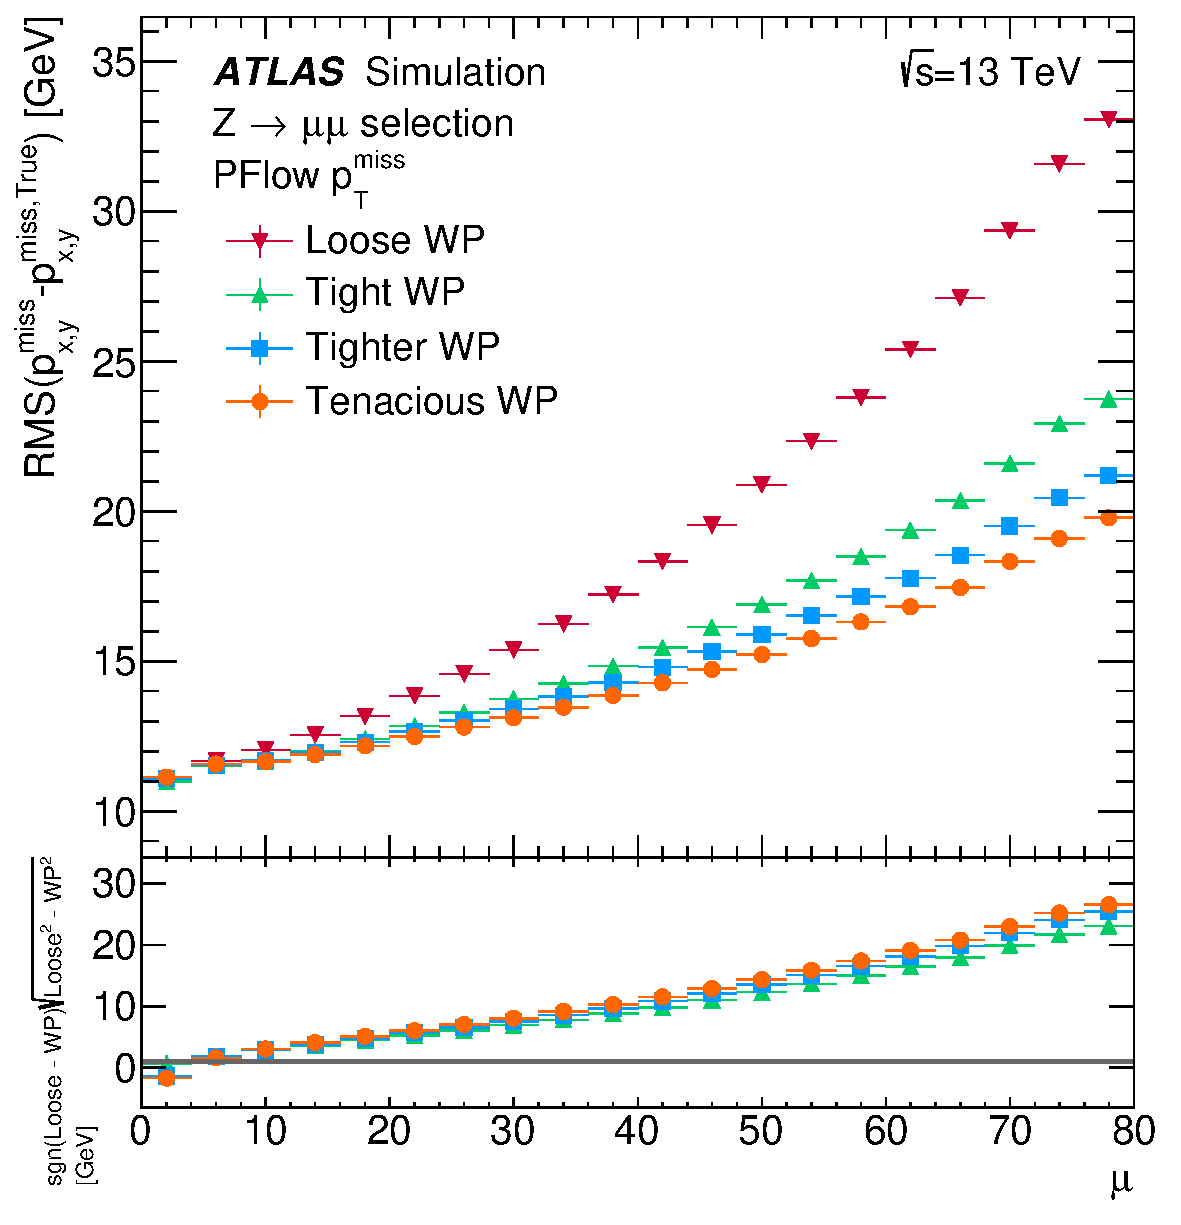
\includegraphics[width=0.495\textwidth]{met_reso_mu.pdf}
                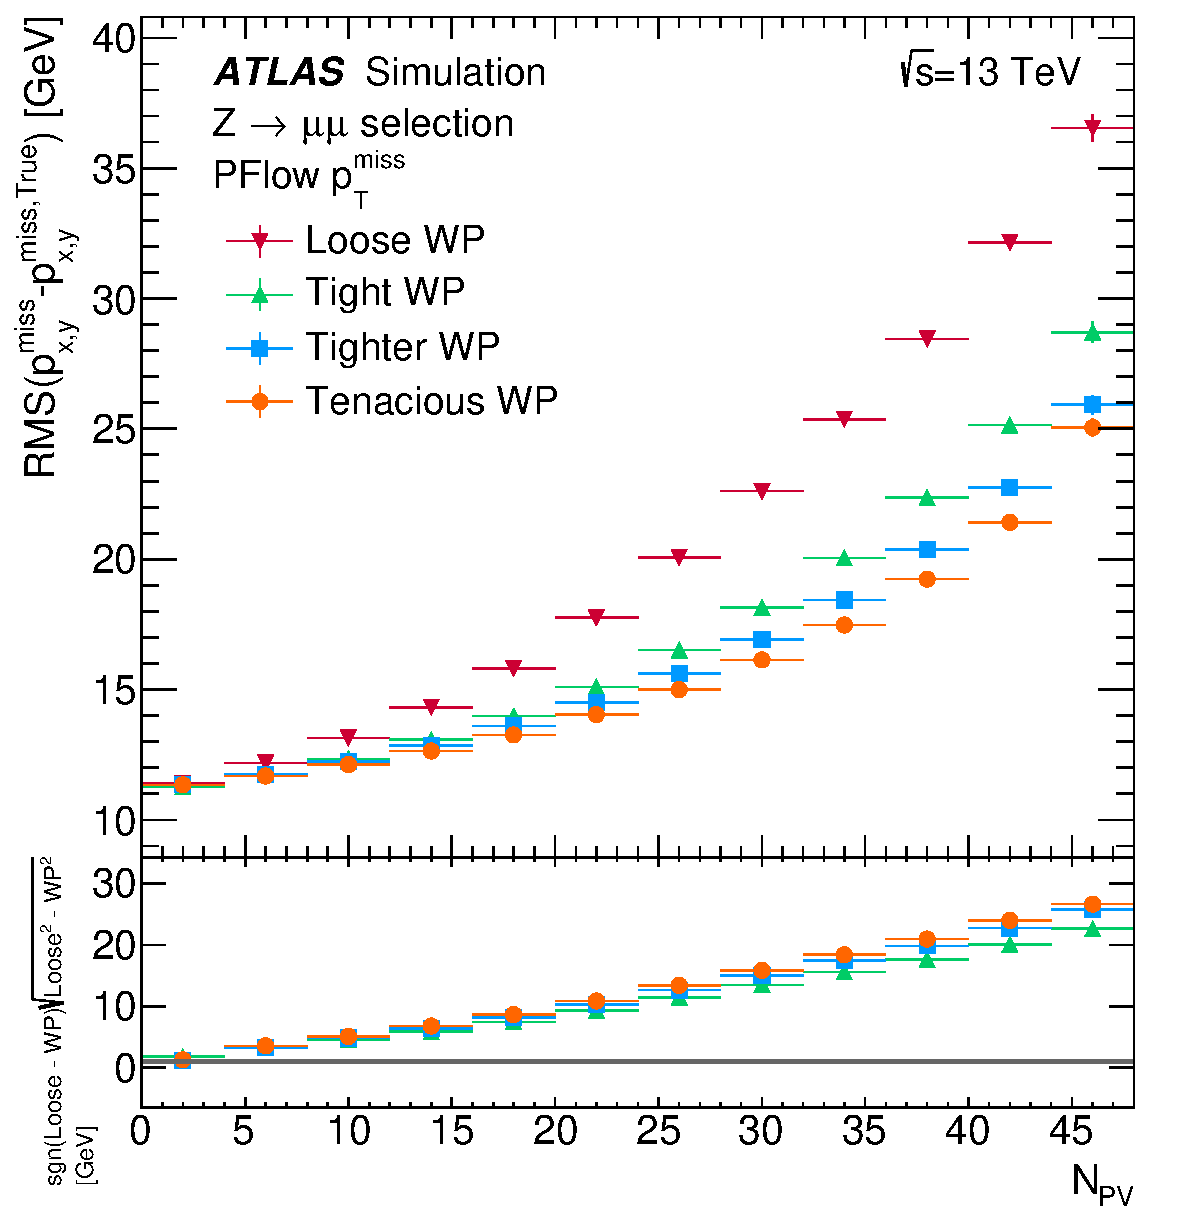
\includegraphics[width=0.495\textwidth]{met_reso_pv.pdf}
                \caption{
                    The $p_x^\text{miss}$ and $p_y^\text{miss}$ resolution for different $p_\text{T}^\text{miss}$ working points as a function of interactions per bunch crossing (left) or number of primary vertices (right). 
                    PFlow jets are used on SM MC simulations with $Z\rightarrow\mu\mu$ events. 
                    These figures are taken from~\cite{JETM-2020-03}.
                }
                \label{fig:met_reso}
            \end{figure}

            
    

    \subsection{Jet flavour tagging}
        The ATLAS experiment employs a sophisticated array of algorithms for identifying jets containing \(b\)-hadrons (b-jets) and \(c\)-hadrons (c-jets), 
        commonly referred to as flavour-tagging algorithms~\cite{FTAG-2019-07,ATL-PHYS-PUB-2022-027}. The core of these algorithms lies in exploiting the unique characteristics of \(b\)- and \(c\)-hadrons, 
        such as their long lifetimes, high masses, and complex decay patterns, to distinguish them from jets originating from lighter quarks. Specialised 
        flavour tagging is also designed to identify large-radius jets originating from boosted Higgs bosons decaying into pairs of bottom quarks (\(H \to b\bar{b}\)) 
        and charm quarks (\(H \to c\bar{c}\))~\cite{ATL-PHYS-PUB-2020-019,ATL-PHYS-PUB-2023-021}. The latest developments in jet flavour tagging employ Graph Neural Networks
        to enhance performance~\cite{ATL-PHYS-PUB-2022-027, ATL-PHYS-PUB-2023-021}.

        \subsubsection{DL1r taggers}
            The Run 2 flavour-tagging strategy of ATLAS is based on a two-stage approach. The first stage involves low-level taggers that reconstruct specific 
            features of heavy-flavour jets using two complementary methods: track-based and vertex-based approaches. Track-based algorithms analyse the 
            properties of individual charged-particle tracks associated with a hadronic jet, while vertex-based algorithms focus on reconstructing displaced 
            vertices from these tracks. Key low-level taggers include:
            \begin{itemize}
                \item Impact Parameter Algorithms (IP2D, IP3D)~\cite{ATL-PHYS-PUB-2017-013}: These algorithms utilise the impact parameters of tracks, which are the distances of 
                closest approach of tracks to the primary vertex. IP2D and IP3D calculate likelihood ratios from the track impact parameter significances, 
                with IP3D additionally considering the 3D impact parameter.
                \item Secondary Vertex Finder (SV1)~\cite{ATL-PHYS-PUB-2017-011}: This algorithm reconstructs secondary vertices within the jet by combining tracks that originate 
                from a common point away from the primary collision vertex. It enhances pile-up rejection and overall performance at high jet \( p_T \) through 
                advanced track-cleaning and vertexing techniques.
                \item JetFitter~\cite{ATL-PHYS-PUB-2018-025}: This algorithm aims to reconstruct the entire decay chain of \(b\)-hadrons within the jet by employing a topological 
                vertex finding approach. It identifies multiple vertices and uses a Kalman filter to improve vertex reconstruction.
                \item RNNIP: A track-based Recurrent Neural Network (RNN) that utilises the sequential nature of track hits to improve the identification 
                of \(b\)- and \(c\)-jets.
            \end{itemize}
            The outputs of the low-level taggers are then fed into high-level taggers, which are multivariate classifiers designed to maximise 
            flavour-tagging performance. The primary high-level tagger used during Run 2 is the DL1~\cite{ATL-PHYS-PUB-2017-013} algorithm series, which employs deep learning techniques.
            DL1 Combines the outputs of IP2D, IP3D, SV1, and JetFitter using a feed-forward neural network.
            DL1r~\cite{ATL-PHYS-PUB-2017-013}is an enhanced version of DL1 that also incorporates the RNNIP outputs. DL1r significantly improves the tagging performance by 
            leveraging the low correlation of RNNIP outputs with other taggers.
            The performance of flavour-tagging algorithms is evaluated in terms of their efficiency to correctly identify \(b\)-jets (\(\epsilon_b\)) 
            and their ability to reject light-flavour jets and \(c\)-jets. The DL1d tagger achieves a light-flavour jet rejection factor of 170 and 
            a charm-jet rejection factor of 5 at a \(b\)-jet identification 
            efficiency of 77\%. For charm-jet identification, DL1r achieves a light-flavour jet rejection factor of 70 and a \(b\)-jet rejection 
            factor of 9 at a charm-jet efficiency of 30\%. The flavour-tagging performance is further assessed across various jet \(p_T\) and \(|\eta|\) 
            ranges, and by ensuring robustness against pile-up interactions. The algorithms maintain consistent performance even with increased pile-up, 
            showing minimal variation in \(b\)-tagging efficiency and background rejection factors across different collision environments.
        
        \subsubsection{GNN-based tagger}
            In Run-3, ATLAS will implement a novel jet tagger using a Graph Neural Network (GNN) architecture known as GN1~\cite{ATL-PHYS-PUB-2022-027, ATL-PHYS-PUB-2023-021}. This advanced method 
            represents a significant departure from traditional flavour tagging approaches, relying on its ability to process information from a 
            variable number of charged particle tracks within a jet without intermediate low-level algorithms. Here, we detail the architecture, 
            implementation, and performance of the GNN-based taggers.
        
            GN1 utilises a sophisticated GNN layer combined with auxiliary training objectives. The primary goal is jet flavour 
            classification, identifying whether jets originate from \(b\)- or \(c\)-quarks. GN1 employs a fully connected graph where each node 
            represents a track within the jet. These nodes are characterised by feature vectors derived from a per-track initialisation network, 
            which then interact within the graph to predict jet flavour, track origins, and vertex groupings. 
            GN1 demonstrates superior performance compared to the current DL1r tagger across various metrics. For jets within the \(t\bar{t}\) 
            sample with transverse momentum (\(p_T\)) between 20 and 250 GeV, GN1 improves light-jet and \(c\)-jet rejection by factors of 
            approximately 1.8 and 2.1, respectively, at a 70\% \(b\)-jet tagging efficiency. In the higher \(p_T\) range (250 < \(p_T\) < 5000 GeV) 
            from the \(Z'\) sample, these improvements rise to factors of around 6 for light-jet rejection and 2.8 for \(c\)-jet rejection at a \(b\)-jet efficiency of 30\%.
            This method's inclusive reconstruction efficiency in \(b\)-jets reaches approximately 80\%, indicating its robust capability to 
            identify displaced vertices from \(b\)-hadron decays.
            GN1 represents a significant advancement in jet flavour tagging for the ATLAS experiment, offering improved performance and flexibility. 
            By eliminating the dependence on low-level algorithms and employing a unified GNN approach, GN1 not only enhances the efficiency of 
            \(b\)- and \(c\)-jet identification but also simplifies the optimisation process for various tagging applications.
            \begin{figure}[htbp]
                \centering
                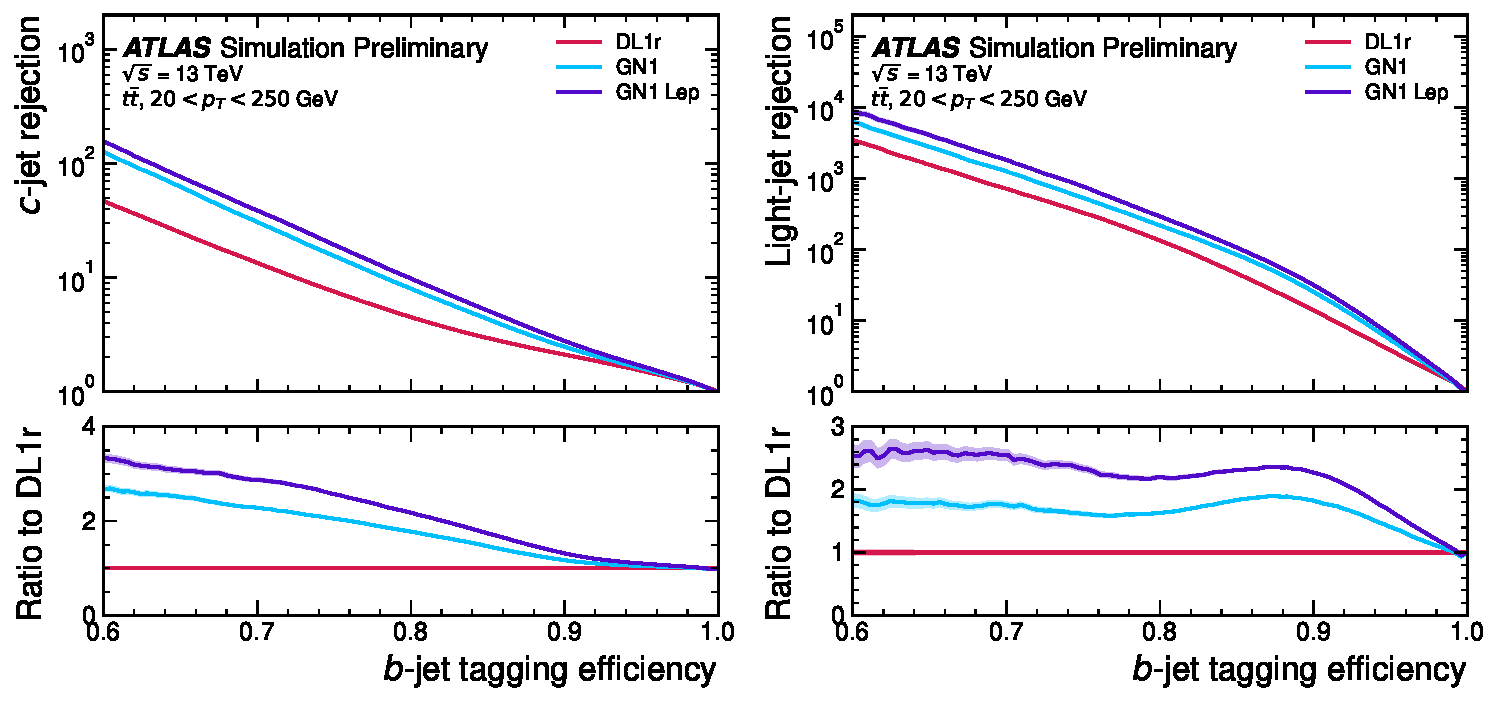
\includegraphics[width=1.0\textwidth]{GN2_roc.pdf}
                \caption{
                    The GN2 c-jet (left) and light-jet (right) rejections as a function of the b-jet tagging efficiency for jets in the $\ttbar$ sample with $20 < \pT < 250$ GeV. 
                    The ratio with respect to the performance of the DL1r algorithm is shown in the bottom panels. 
                    These figures are taken from~\cite{ATL-PHYS-PUB-2022-027}.
                }
                \label{fig:GN2_roc}
            \end{figure}
        
        \subsubsection{GNN-based flavour tagging for large-R jets}
            In Run 3, ATLAS advanced its flavour tagging capabilities with the development of the GN2X~\cite{ATL-PHYS-PUB-2023-021} algorithm, designed to 
            identify large-radius jets originating from boosted Higgs bosons decaying into pairs of bottom quarks (\(H \to b\bar{b}\)) and charm quarks 
            (\(H \to c\bar{c}\)). The GN2X algorithm leverages recent advancements in GNNs and transformer architectures, 
            providing significant improvements in background rejection and tagging efficiency compared to previous methods.
            
            The base GN2X model takes three large-radius jet variables and 20 track variables as inputs. Up to 100 tracks per 
            jet are considered, sorted by decreasing transverse impact parameter significance to prioritise tracks from displaced vertices.
            The GN2X architecture utilises a transformer network with multiple encoder blocks and attention 
            heads~\cite{shleifer2021normformerimprovedtransformerpretraining, ba2016layernormalization} to process the track 
            representations. This setup allows the model to capture complex relationships among tracks and derive a global jet representation for classification.
            In addition to the primary jet classification task, GN2X includes auxiliary training objectives for track origin 
            classification and vertex grouping, enhancing the model's ability to identify displaced vertices and improve tagging performance.
            GN2X achieves significant improvements in background rejection compared to previous taggers in \(H \to b\bar{b}\) tagging. At a 
            50\% \(H(b\bar{b})\) tagging efficiency, GN2X provides a background rejection factor of 40 for jets from top quark decays and 300 
            for multijet events. This represents a factor of 1.6 improvement in top jet rejection and a factor of 2.5 improvement in multijet 
            rejection compared to the baseline tagger $D_\mathrm{xbb}$~\cite{FTAG-2019-07}.
            For \(H(c\bar{c})\) tagging, GN2X offers substantial enhancements in rejecting background jets, including those from \(H(b\bar{b})\) 
            decays. At a 50\% \(H(c\bar{c})\) tagging efficiency, GN2X achieves a factor of 3 improvement in top jet rejection, 
            a factor of 5 improvement in multijet rejection, and a factor of 6 improvement in \(H(b\bar{b})\) rejection.
            GN2X maintains stable tagging efficiency across the entire transverse momentum (\(p_T\)) spectrum of the jets. At a 50\% 
            \(H(b\bar{b})\) efficiency working point, GN2X shows consistent performance, significantly outperforming the baseline taggers 
            across all \(p_T\) ranges. The algorithm exhibits less efficiency drop-off at high \(p_T\) compared to previous methods, 
            ensuring reliable performance even for high-energy jets.
            \begin{figure}[htbp]
                \centering
                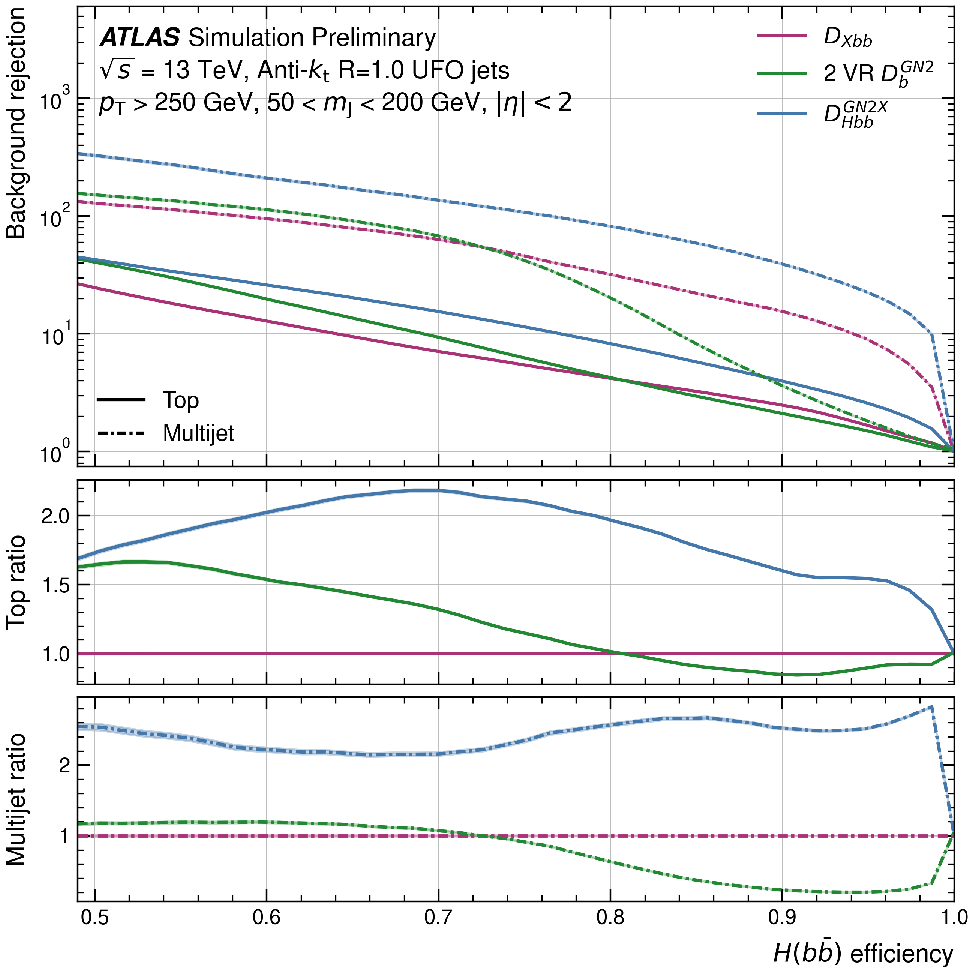
\includegraphics[width=0.5\textwidth]{GN2x_roc.pdf}
                \caption{
                    GN2x top and multijet rejections as a function of the $H\rightarrow bb$ efficiency for jets with $\pt>250$ GeV and mass ($50~\GeV < m_J < 200~\GeV$). 
                    Performance of the GN2X algorithm is compared to the previous DXbb tagger and variable-radius subjets baselines.
                    These figures are taken from~\cite{ATL-PHYS-PUB-2023-021}.
                }
                \label{fig:GN2x_roc}
            \end{figure}


    \subsection{Muon reconstruction and identification}
        The muon reconstruction and identification process~\cite{MUON-2018-03} involves several sophisticated techniques that use the 
        capabilities of the ATLAS detector's subsystems, including the Inner Detector (ID), Muon Spectrometer (MS), 
        and calorimeters.
        
        \subsubsection{Muon reconstruction}
            Muon reconstruction in ATLAS primarily exploits the characteristics of minimum-ionising particles. This involves the identification of 
            tracks within the MS or through specific energy deposits in the calorimeters. The reconstruction process utilises data from both the 
            ID and MS tracking detectors, with calorimeter information contributing to track parameter determination and tagging of muon candidates 
            independently from the MS.
        
            The MS Stand-Alone Reconstruction process starts by identifying short straight-line segments from hits in individual MS stations using 
            a Hough transform. These segments are combined into track candidates, taking into account the initial pointing constraint and the 
            parabolic trajectory of the muon bending in the magnetic field. A global $\chi^2$ fit of the muon trajectory is then performed, 
            which considers possible interactions with detector material and misalignments between detector chambers. Outliers are removed, 
            and missing hits are added to refine the track fit. The final track is extrapolated back to the beam line, with its \pT expressed 
            at the interaction point (IP). Global Muon Reconstruction involves a combination of information from the ID, MS, and calorimeters. 
            The process follows five main strategies, resulting in different types of muons: Combined (CB), Inside-Out (IO), Muon-Spectrometer 
            Extrapolated (ME), Segment-Tagged (ST), and Calorimeter-Tagged (CT)~\cite{MUON-2018-03}. Each type has its reconstruction pathway, which includes 
            matching MS tracks to ID tracks, extrapolating ID tracks to the MS, or using calorimeter data to tag muons.
        
        \subsubsection{Muon identification}
            Different WPs are defined based on the required efficiency, resolution, and background rejection. These criteria are applied to hits 
            in the ID and MS, track fit properties, and compatibility variables between detector measurements. The WPs are tailored to optimise 
            performance for various physics analyses, targeting prompt-muon identification, momentum resolution, and non-prompt muon rejection.
            The tag-and-probe method uses dimuon pairs from $Z\rightarrow \mu^+\mu^-$ decays to measure reconstruction and identification 
            efficiencies. One muon (the tag) must satisfy stringent criteria and trigger the event-selection, while the other (the probe) tests 
            the efficiency of specific algorithms. Several probe types (ID, MS, CT, ST) are used to measure various efficiencies, and a matching 
            requirement of $\Delta R < 0.05$ is applied to ensure accurate efficiency measurements. Efficiency scale factors are derived to correct 
            simulation data to match real detector performance.
            \begin{figure}[htbp]
                \centering
                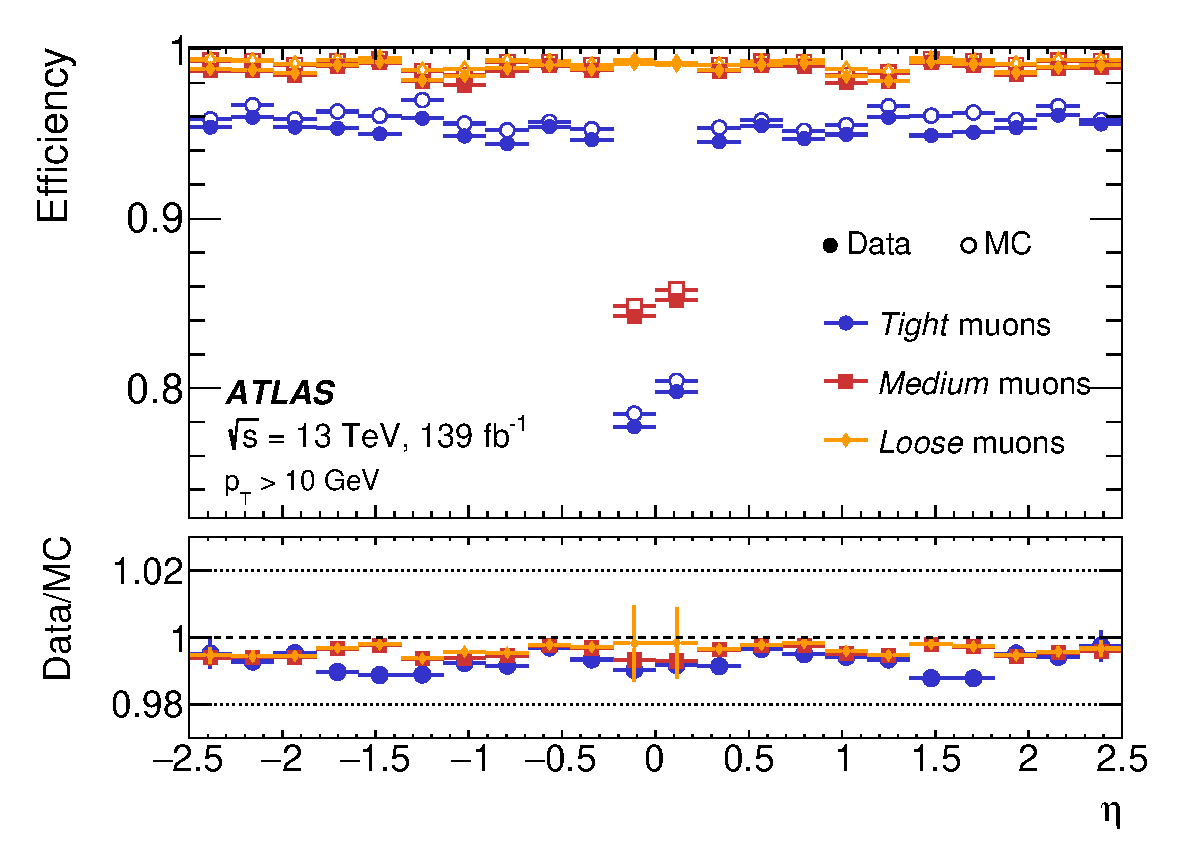
\includegraphics[width=0.6\textwidth]{muon_effi_eta.pdf}
                \caption{
                    Muon reconstruction and identification efficiencies for the Loose, Medium, and Tight criteria. It displays the efficiencies measured in $Z\rightarrow\mu\mu$ events as a function of $\eta$, for muons with $\pt>10$~GeV. 
                    This figure is taken from~\cite{MUON-2018-03}.
                }
                \label{fig:muon_effi}
            \end{figure}
        
        \subsubsection{Muon calibration}
            Muon momentum calibration~\cite{MUON-2022-01} is critical for achieving precise measurements, especially given the complexities of the detector geometry and alignment.
            Biases introduced by residual misalignments in the detector are corrected using a charge-dependent momentum calibration technique. This method
            involves analysing the mass of the dimuon system from Z$\rightarrow \mu^+\mu^-$ decays to estimate and correct biases in the muon momentum
            scale. The calibration procedure is validated using independent samples of J/$\psi\rightarrow\mu^+\mu^-$ and $\Upsilon\rightarrow\mu^+\mu^-$ decays.
            These procedures include detailed studies of detector response, alignment system uncertainties, and the development of correction factors for both the ID and MS.
            The ultimate goal is to minimise the systematic uncertainties and achieve the highest possible precision in momentum measurement.
        
    \subsection{$\tau$ lepton reconstruction}
        A $\tau$ lepton has a 35\% probability of decaying leptonically to a lighter lepton ($\tau_\mathrm{e}$ or $\tau_\mathrm{\mu}$) and two neutrinos. 
        In the remaining 65\% of cases a $\tau$ lepton decays hadronically ($\tauhad$) to one or more charged hadrons, zero or more
        neutral hadrons, plus one neutrino. 
        The leptonically decaying $\tau$ leptons are reconstructed as prompt electrons or muons in the ATLAS detector with non-zero impact parameters. 
        The visible part of the hadronically decaying $\tau$ leptons ($\tauhadvis$) are reconstructed and identified using a combination of tracking and calorimetric information. 

        A significant portion of this thesis is dedicated to the detailed reconstruction and identification of $\tauhadvis$. 
        This constitutes a major part of the research I have been worked on. 
        The next chapter will delve deeply into this topic, providing comprehensive insights and methodologies.
    %!TEX root = ../thesis.tex

\chapter{The $\tauhadvis$ reconstruction and identification at ATLAS}

\graphicspath{{1_MainChapters/Chap4_TauRec/figs}}
    This chapter describes the reconstruction (TauReco) and identification (TauID) of hadronically decaying tau leptons ($\tauhadvis$),
    largely based on the ``Reconstruction, Identification, and Calibration of hadronically decaying tau leptons 
    with the ATLAS detector for the LHC Run~3 and reprocessed Run~2 data''~\cite{ATL-PHYS-PUB-2022-044}. Over the 
    years, TauReco and TauID has been significantly improved, starting from 
    a cut-based approach adopted during early Run 1~\cite{ATL-PHYS-PUB-2010-001}, to a boosted decision tree (BDT)
    algorithm from the end of Run 1~\cite{PERF-2013-06}, and finally to a recurrent neural network (RNN) algorithm
    during Run 2 and Run 3~\cite{ATL-PHYS-PUB-2022-044}. In the future, TauID will be further improved by
    incorporating more advanced machine learning techniques such as graph neural networks (GNNs) and transformers.
    Early results from the GNN-based TauID have shown promising performance, with the potential to further enhance
    the signal-to-background separation in the $\tauhadvis$ identification.

\section{$\tauhadvis$ reconstruction}
    The candidates for $\tauhadvis$ are initially seeded by jets formed using the 
    anti-\(k_T\) algorithm, which has a radius parameter of $R = 0.4$. 
    The TopoClusters are calibrated using a local hadronic calibration (LC). 
    Jets that seed $\tauhadvis$ candidates must have \pt greater than 5 GeV and $|\eta| < 2.5$. 
    The \pT requirement is applied to the LC energy of the jet, prior to any JES corrections. 

    \subsection{Vertex association}
        During p-p collisions at the LHC, multiple simultaneous interactions occur, resulting in the reconstruction 
        of several interaction vertices. Typically, particles are assumed to originate from the primary vertex, 
        which is defined as the vertex with the highest sum of the squared transverse momenta of the associated 
        tracks (\(\sum p_T^2\)). However, since tau leptons decay away from the primary vertex, a dedicated 
        tau vertex association algorithm (TJVA) is used to identify the correct production vertex for each 
        $\tauhadvis$ candidate. This production vertex is then used for $\tauhadvis$
        reconstruction instead of the primary vertex.
        
        The tau production vertex is crucial for calculating quantities such as the impact parameter and determining 
        which tracks are associated with the $\tauhadvis$ candidate. Parameters of the associated 
        tracks are recalculated relative to the tau production vertex.
        
        For Run 3, the vertexing algorithm has been updated to handle the high pile-up environment, necessitating 
        a re-tuning of the TJVA. The method is based on the \pt fraction of a given vertex $f_{\pt}$:
        \[ f_{\pt} = \frac{\sum \pt (\text{tracks associated with the vertex})}{\sum \pt (\text{all tracks})} \]
        where all tracks within (\(\Delta R\)) of less than 0.2 from the seed jet are considered. The vertex 
        with the highest $f_{\pt}$ fraction is chosen as the tau production vertex and is used for determining 
        the $\tauhadvis$ direction, associating tracks, and building the coordinate system for calculating 
        identification variables.
        
        The efficiency of selecting the correct tau production vertex compared to the primary vertex is evaluated 
        as a function of the \tauhadvis \pt and the average number of simultaneous proton-proton 
        collisions ($\langle \mu \rangle$). The tau production vertex consistently shows better efficiency, 
        especially at low \pt.
        
        The $\tauhadvis$ four-momentum is calculated by first computing \(\eta\) and \(\phi\) of 
        the barycentre of the TopoClusters of the seed jet, calibrated at the LC scale, assuming a mass of zero 
        for each constituent. The four-momenta of all clusters in the region \(\Delta R < 0.2\) around the 
        barycentre are recalculated using the tau production vertex coordinate system and summed, providing 
        the momentum magnitude and direction of the $\tauhadvis$. Figure \ref{fig:tau_vtx_eff} shows the 
        efficiency to select the correct $\tau$ production vertex using TJVA or the default primary vertex
        in $\gamma^*\rightarrow\tau\tau$ events, as a function of $\langle \mu \rangle$, taken from~\cite{ATL-PHYS-PUB-2022-044}.
        \begin{figure}[htbp]
            \centering
            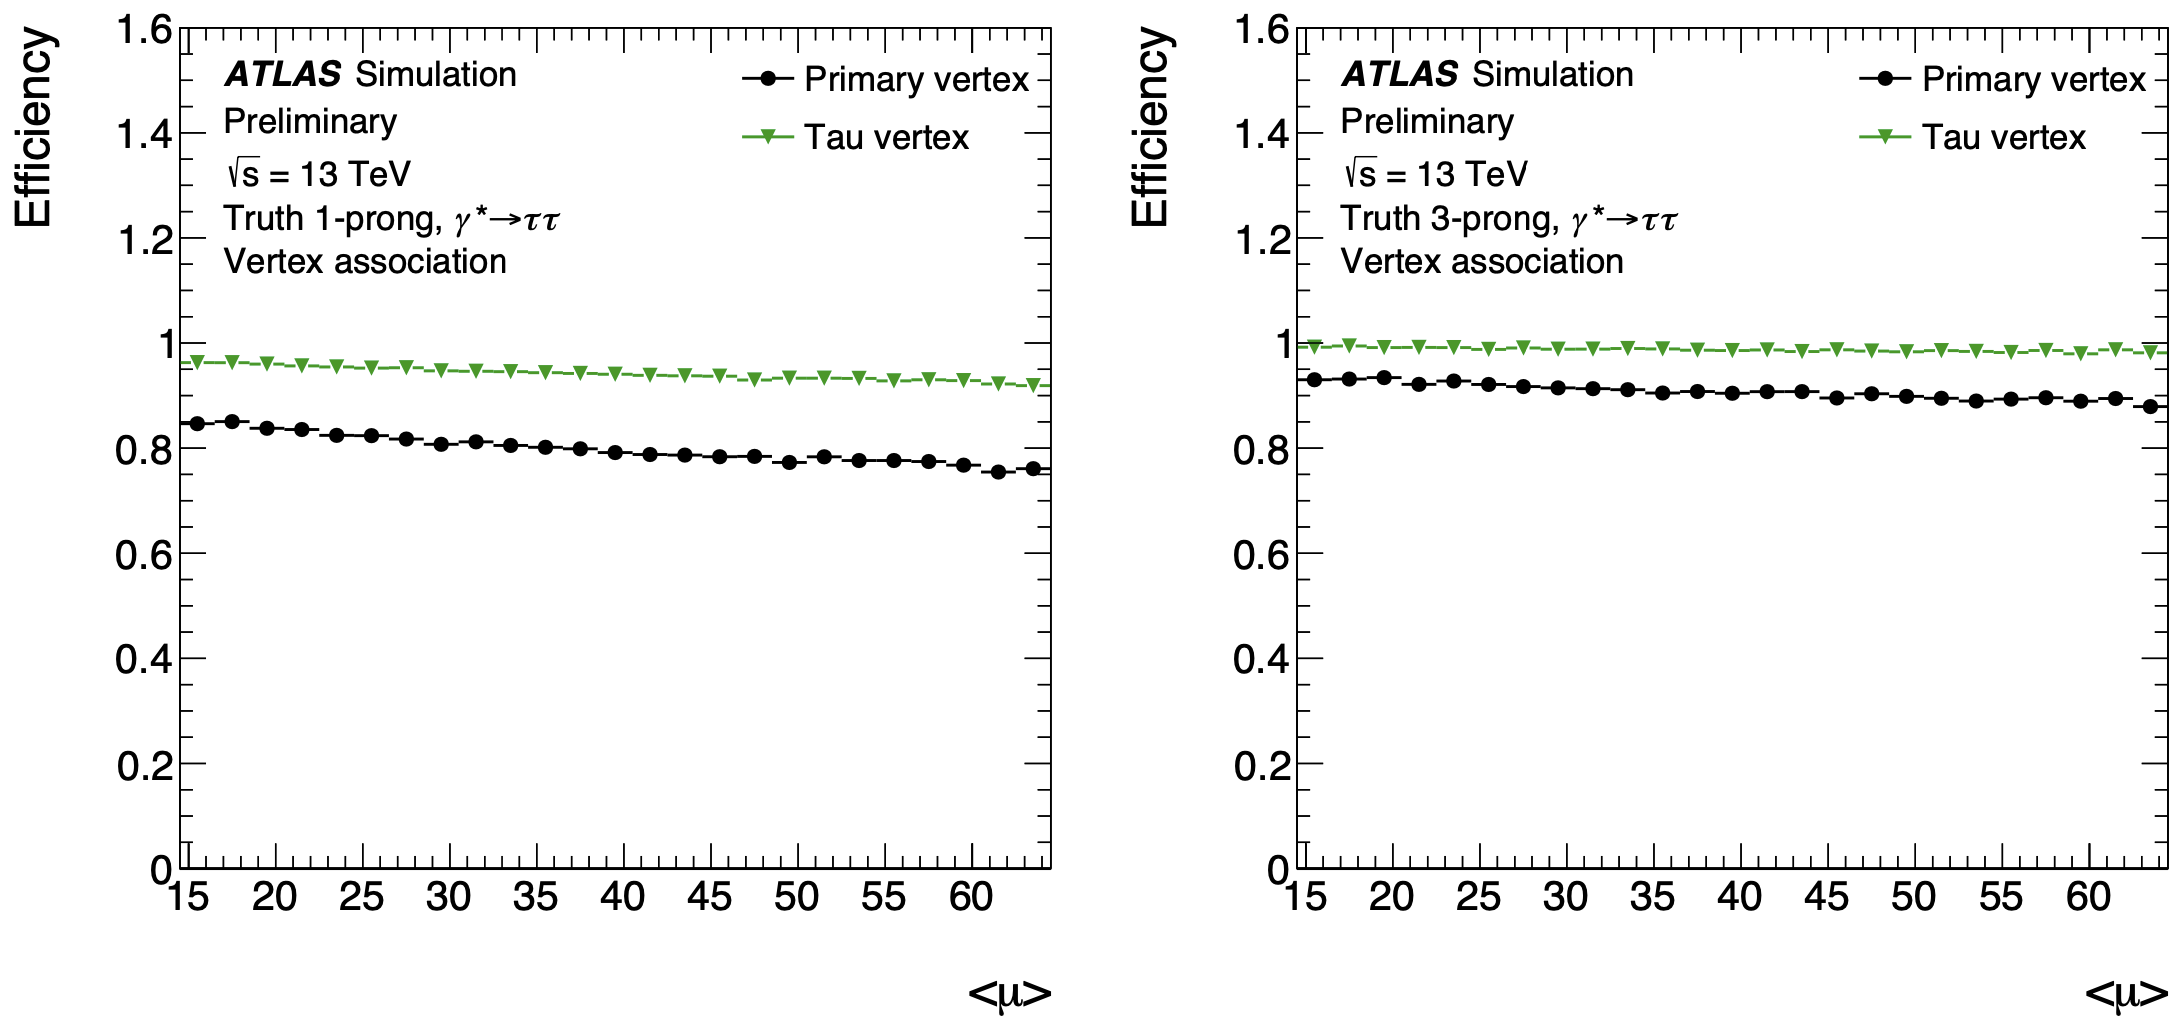
\includegraphics[width=0.9\textwidth]{vtx_tagging}
            \caption{
                Efficiency to select the correct $\tau$ production vertex using TJVA or the default primary vertex in $\gamma^*\rightarrow\tau\tau$ events, as a function of $\langle \mu \rangle$. 
                The left plot shows the efficiency for 1-prong $\tauhad$, while the right plot shows the efficiency for 3-prong $\tauhad$, taken from~\cite{ATL-PHYS-PUB-2022-044}.
            }
            \label{fig:tau_vtx_eff}
        \end{figure}
        
    \subsection {Track Association}
        Tracks are associated with the $\tauhadvis$ candidate if they are within a core region 
        (\(\Delta R < 0.25\)) around the $\tauhadvis$ direction and meet the following criteria:
        \begin{itemize}
            \item \pt greater than 1 GeV,
            \item at least two associated hits in the pixel layers of the inner detector,
            \item at least seven hits in total in the pixel and SCT layers.
        \end{itemize}
        Additionally, association requirements are imposed on the distance of closest approach of the track 
        to the tau production vertex in the transverse plane (\(|d_{0}^{\text{TJVA}}| < 1.0\) mm) and 
        longitudinally (\(|z_{0}^{\text{TJVA}} \sin \theta | < 1.5\) mm).
        Tracks in the region \(0.25 < \Delta R < 0.4\) are also associated with the $\tauhadvis$if either:
        \begin{itemize}
            \item they are matched to the \tauseed jet by a ghost-particle association technique, or
            \item the closest jet to the track in terms of \(\Delta R\) distance is the $\tauhadvis$ seeding jet.
        \end{itemize}
    
    \subsection {Track Classification}
        To correctly establish the charge and the number of charged decay products of a tau lepton, the tracks that are 
        associated with the tau decay need to be correctly distinguished from the other tracks associated with the \tauseed. 
        Using a track classifier, tracks that have passed the TJVA requirements are classified into four categories:
        \begin{itemize}
            \item tau tracks (TT): tracks originating from charged tau lepton decay products.
            \item conversion tracks (CT): tracks from electrons and positrons that are created from photon conversion in the detector.
            \item isolation tracks (IT): tracks likely originating from quark or gluon jets arising from the remnants of the hard scattering interactions.
            \item fake tracks (FT): tracks that do not belong to the previous categories, mainly misreconstructed tracks and pile-up tracks.
        \end{itemize}
        A novel approach for the tau lepton track classification using a recurrent neural network 
        (RNN)~\cite{schmidt2019recurrentneuralnetworksrnns} has been developed, 
        replacing the previous BDT-based method used during Run 2. RNNs are specifically chosen for their ability to use 
        bidirectional long short-term memory (BLSTM) cells, 
        allowing information to be back-propagated, exploiting 
        forward and backward correlations in sequences of tracks belonging to tau decays.
    
        % The RNN architecture includes three dense layers connected to the input (tracks of the $\tauhadvis$ candidate). 
        % Three BLSTM layers are configured between the dense layers. And one output layer was configured, comprising four nodes, each associated 
        % with a track classifier category. 
        The network is trained using Keras~\cite{chollet2015keras} and TensorFlow~\cite{tensorflow2015-whitepaper}, 
        applied to sequences of \pt-ordered tracks associated with 
        each $\tauhadvis$ candidate. The training data includes signal candidates from simulated \(\gamma^* \rightarrow \tau\tau\) 
        events and background candidates from dijet events, with each sample divided into subsets for training, validation, and performance evaluation. 
        Input variables for the RNN include kinematic, geometric, and detector hit distribution information for the tracks. 
        The primary measure to evaluate the performance of the track classifier are the reconstruction efficiency.
        The reconstruction efficiency is the efficiency to correctly classify 1- or 3-tracks originating from truth 1-prong and 3-prong \(\tau\) leptons.
        The reconstruction efficiency evaluated as a function of the $\tauhadvis$ $pT$ and $\langle \mu \rangle$ is shown in Figure \ref{fig:track_classification_eff}.
        \begin{figure}[htbp]
            \centering
            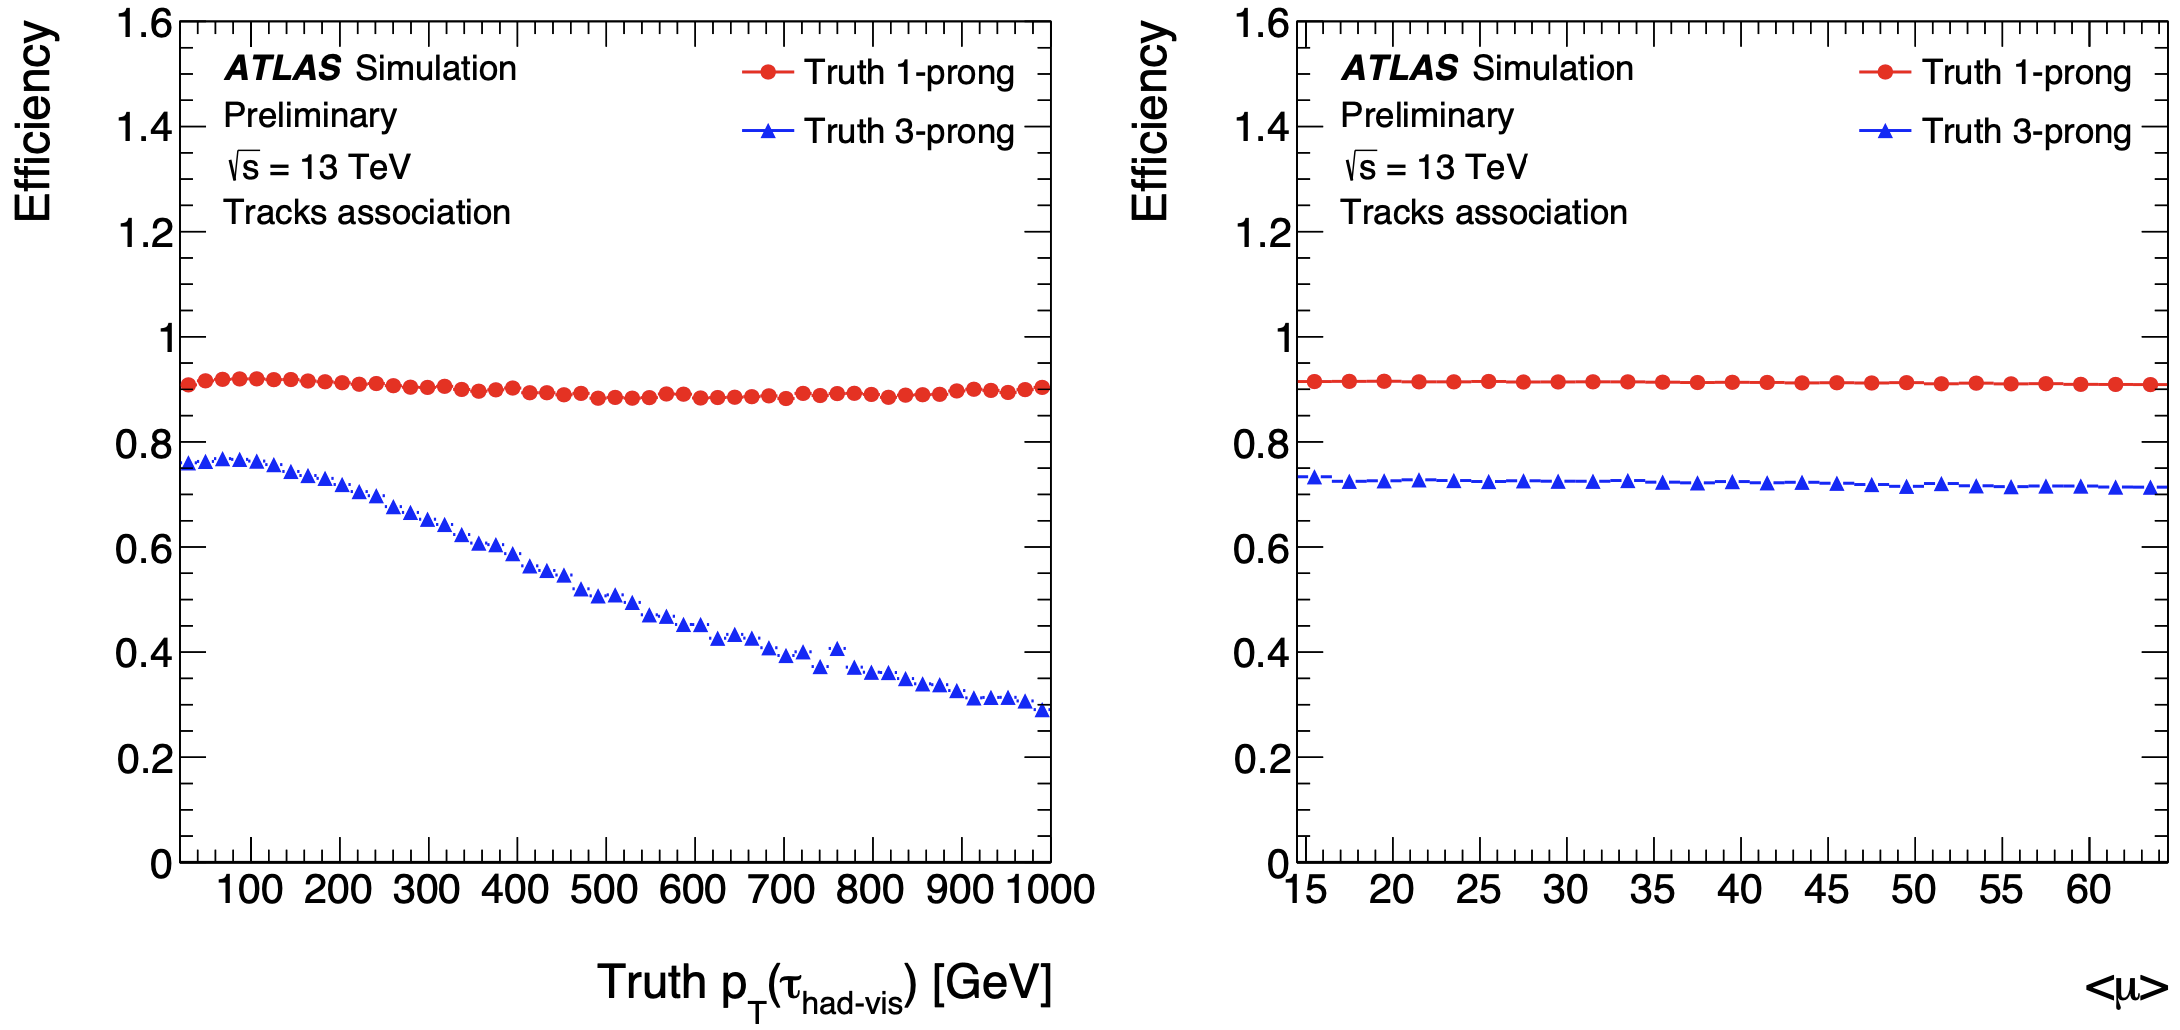
\includegraphics[width=0.9\textwidth]{taureco_eff.png}
            \caption{
                Reconstruction efficiency of the track classifier for 1-prong and 3-prong $\tauhadvis$ candidates as a function of $\tauhadvis p_T$ (left) and $\langle \mu \rangle$ (right).
            }
            \label{fig:track_classification_eff}
        \end{figure}
\section{$\tauhadvis$ Identification and electron-veto}
    \subsection{RNN-based identification}
        During Run 2, a novel $\tauhadvis$ identification algorithm (TauID)
        was introduced to separate true $\tauhadvis$ candidates 
        from those misidentified as originating from quark- and gluon-initiated 
        jets. This algorithm, based on a RNN, utilises information from reconstructed 
        charged-particle tracks and clusters of energy in the calorimeter associated 
        with $\tauhadvis$ candidates, along with high-level discriminating 
        variables. Compared to the BDT identification algorithm used at the 
        beginning of Run 2, the RNN algorithm improved the rejection of 
        misidentified $\tauhadvis$ candidates by 75-100\%, 
        depending on the $\tauhadvis$\pt and the number of tracks.

        The RNN architecture used for $\tauhadvis$ identification consists of three input branches.
        \begin{itemize}
            \item Track Variables: this branch processes information related to the tracks associated with the $\tauhadvis$candidate.
            \item Cluster Variables: this branch processes information related to the energy clusters in the calorimeter.
            \item High-Level Jet Variables: this branch processes high-level observables calculated from track and calorimeter quantities.
        \end{itemize}
        The RNN's internal state allows it to process sequences of unknown length, making it suitable for the variable-length
        input data associated with $\tauhadvis$ candidates. 
        Each branch feeds into the RNN, which is trained using simulated samples of $\tauhadvis$ candidates. 
        The signal sample consists of $\tauhadvis$ candidates from \(\gamma^* \rightarrow \tau\tau\) events,
        while the background sample consists of candidates from simulated QCD di-jet events.
        Reconstructed $\tauhadvis$ candidates from \(\gamma^* \rightarrow \tau\tau\) events are required to 
        be geometrically matched to $\tauhadvis$ at the truth level and correctly reconstructed as 1- or 3-prong decays. 
        Reconstructed $\tauhadvis$ candidates from simulated di-jet samples are required to be reconstructed as 1- or 
        3-prong $\tauhadvis$ candidates.

        The performance of the RNN-based $\tauhadvis$ identification algorithm is evaluated on independent 
        test samples of signal and background events. The efficiency of $\tauhadvis$ identification is 
        measured as a function of \tauhadvis \pT and $\langle \mu \rangle$.

        The identification algorithm defines several working points (Very Loose, Loose, Medium, Tight) based on the 
        transformed (flattened) RNN score, which ensures that the $\tauhad$ efficiency does not depend 
        on the reconstructed \tauhadvis \pT and \(\langle \mu \rangle\). The rejection of misidentified 
        $\tauhadvis$ candidates, defined as the inverse of the background selection efficiency, is evaluated 
        for each working point. The combined reconstruction and identification efficiency of the $\tauhadvis$
        identification algorithm is shown in Figure \ref{fig:tau_id_eff}. 
        Inverse of the efficiency (rejection) for misidentified 1-prong and 3-prong $\tauhad$ candidates from dijet
        background events as a function of the efficiency for truth $\tauhad$ originating from $\gamma^*\rightarrow\tau\tau$ 
        events is shown in Figure~\ref{fig:tau_id_roc}. 
        Both figures are taken from~\cite{ATL-PHYS-PUB-2022-044}.
        \begin{figure}[htbp]
            \centering
            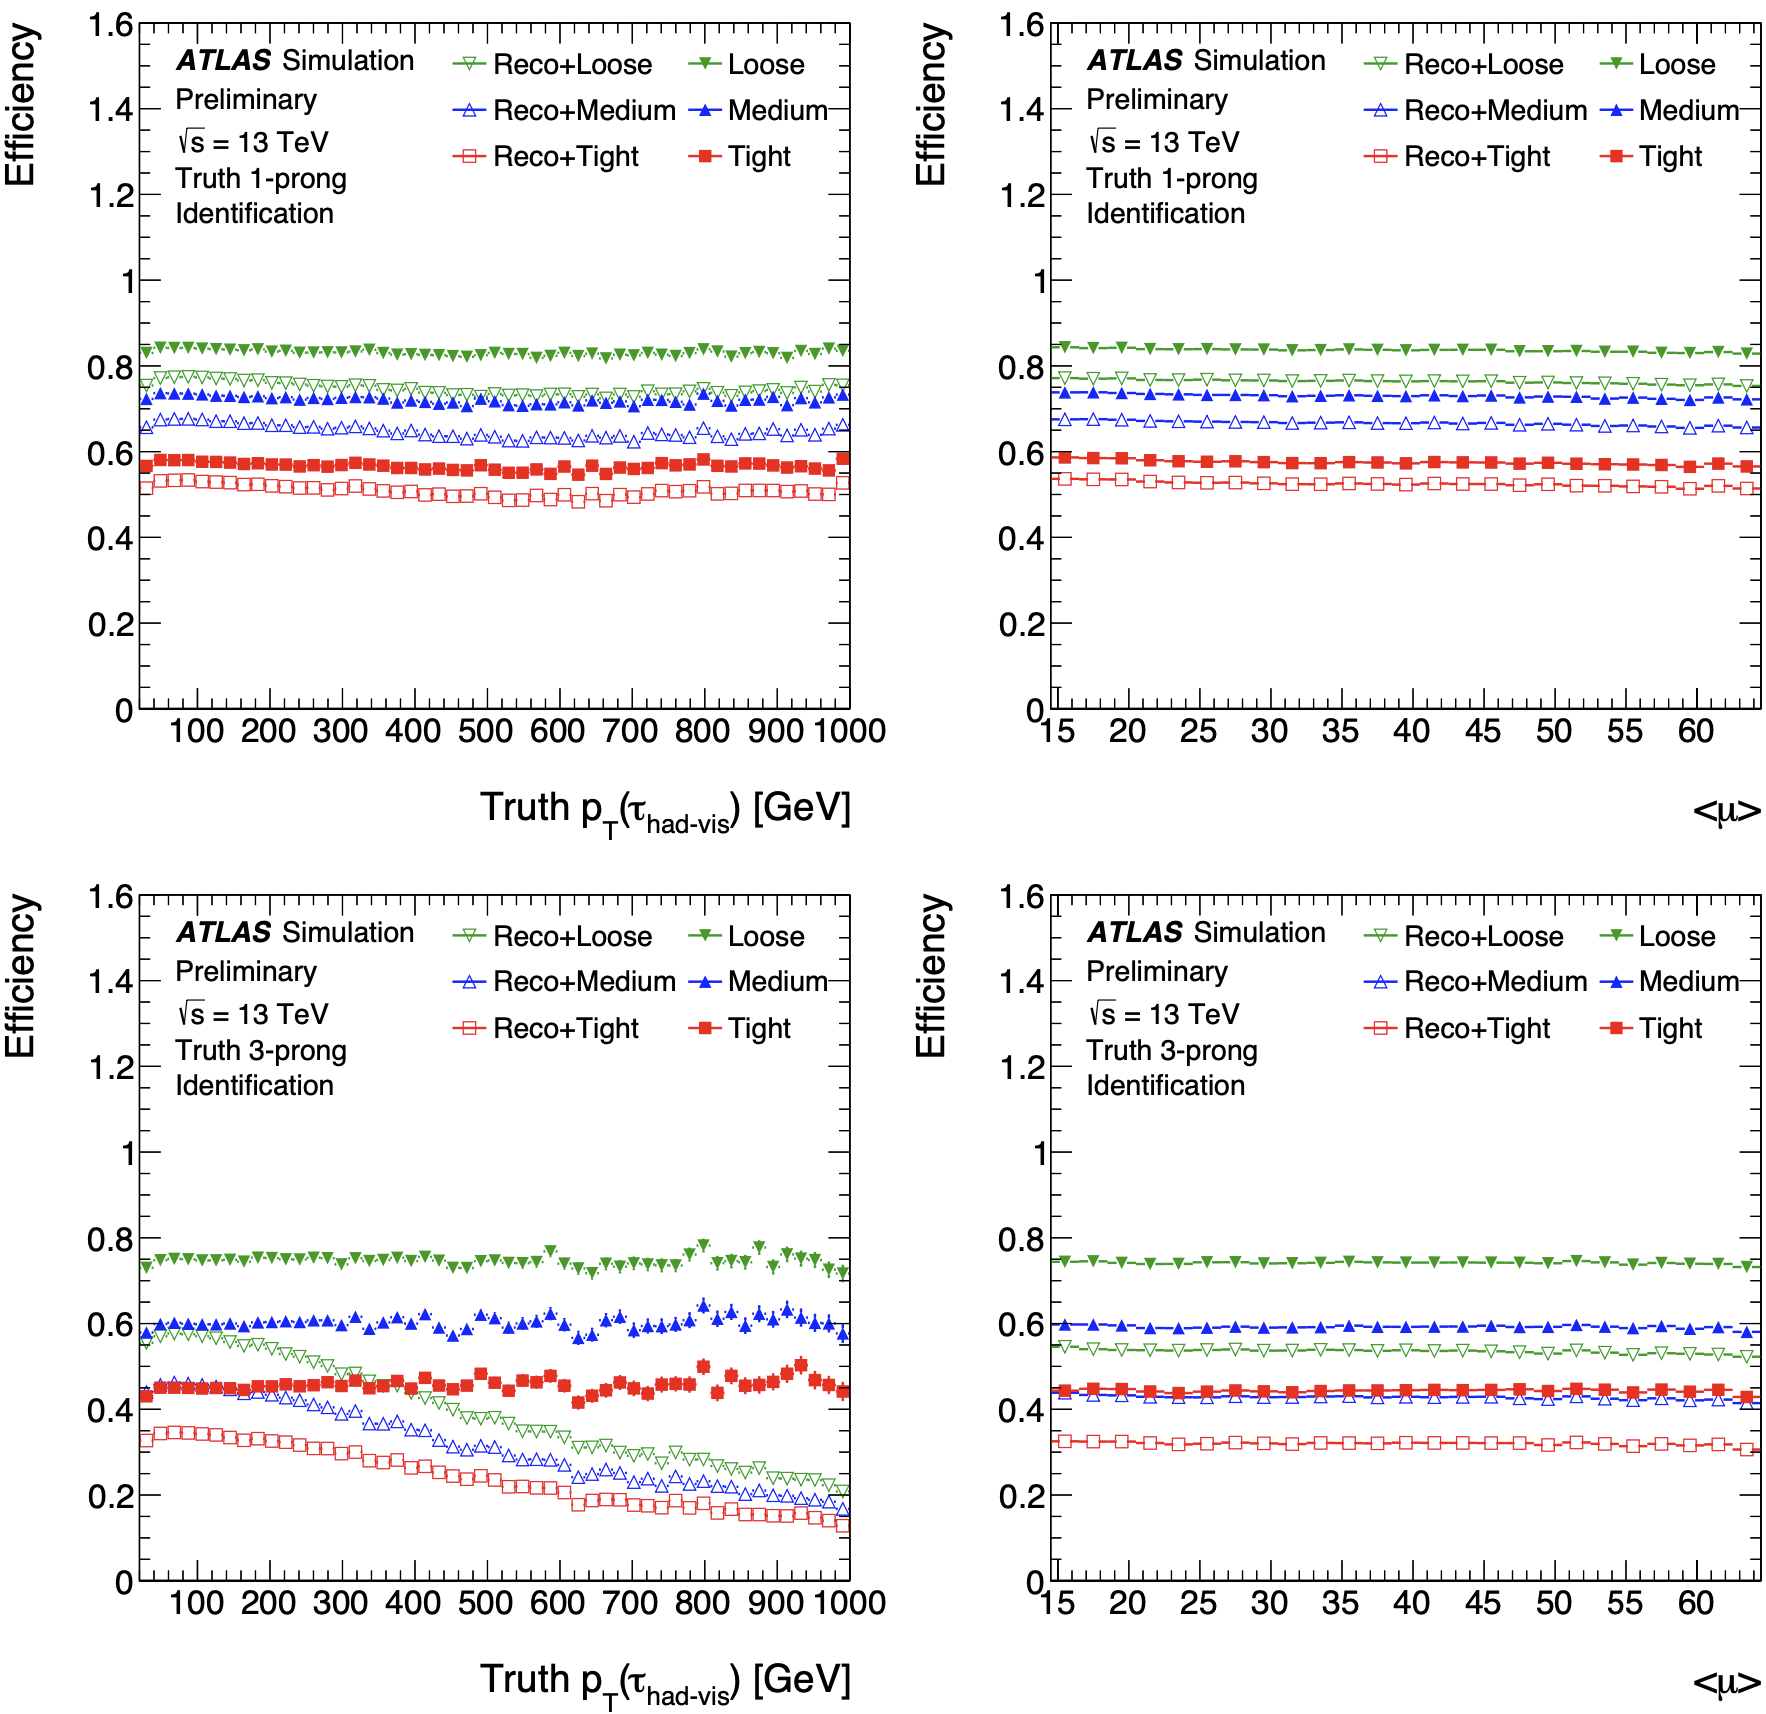
\includegraphics[width=0.9\textwidth]{tauID_eff.png}
            \caption{
                Combined reconstruction and identification efficiency of the $\tauhadvis$ identification algorithm as a 
                function of $\tauhadvis p_T$ (left) and $\langle \mu \rangle$ (right), taken from~\cite{ATL-PHYS-PUB-2022-044}.
                The decay of the $\tauhadvis$ efficiency in 3-prong $\tauhadvis$ candidates at high $\tauhadvis p_T$ is due to the
                tracking efficiency in dense environments.
            }
            \label{fig:tau_id_eff}
        \end{figure}
        \begin{figure}[htbp]
            \centering
            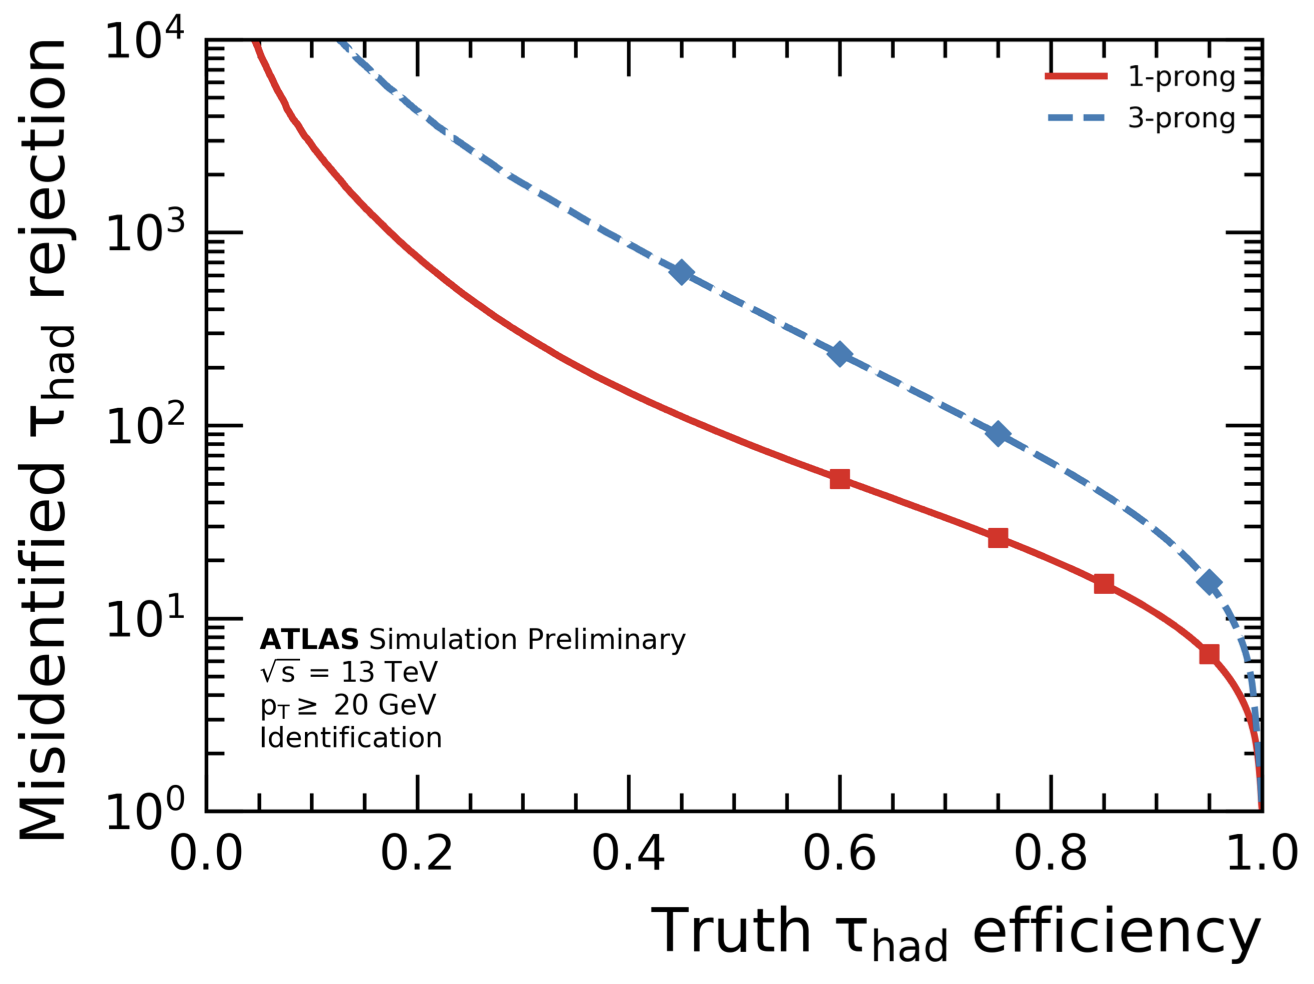
\includegraphics[width=0.45\textwidth]{tauid_roc.png}
            \caption{
                Inverse of the efficiency (rejection) for misidentified 1-prong and 3-prong $\tauhad$ candidates from dijet
                background events as a function of the efficiency for truth $\tauhad$ originating from $\gamma^*\rightarrow\tau\tau$ events, 
                taken from~\cite{ATL-PHYS-PUB-2022-044}.
            }
            \label{fig:tau_id_roc}
        \end{figure}

        The $\tauhad$ candidates are further classified into five primary decay modes by a DeepSet Neural Network (DSNN)~\cite{zaheer2018deepsets} algorithm.
        This method identifies the number of charged and neutral hadrons from $\tau$ decays. The efficiency matrix for reconstructing the same $\tau$ 
        lepton decay mode as the truth decay mode with DeepSet NN classifier in $\gamma^*\rightarrow\tau\tau$ events is shown in Figure \ref{fig:tau_decay_mode_eff}.
        \begin{figure}[htbp]
            \centering
            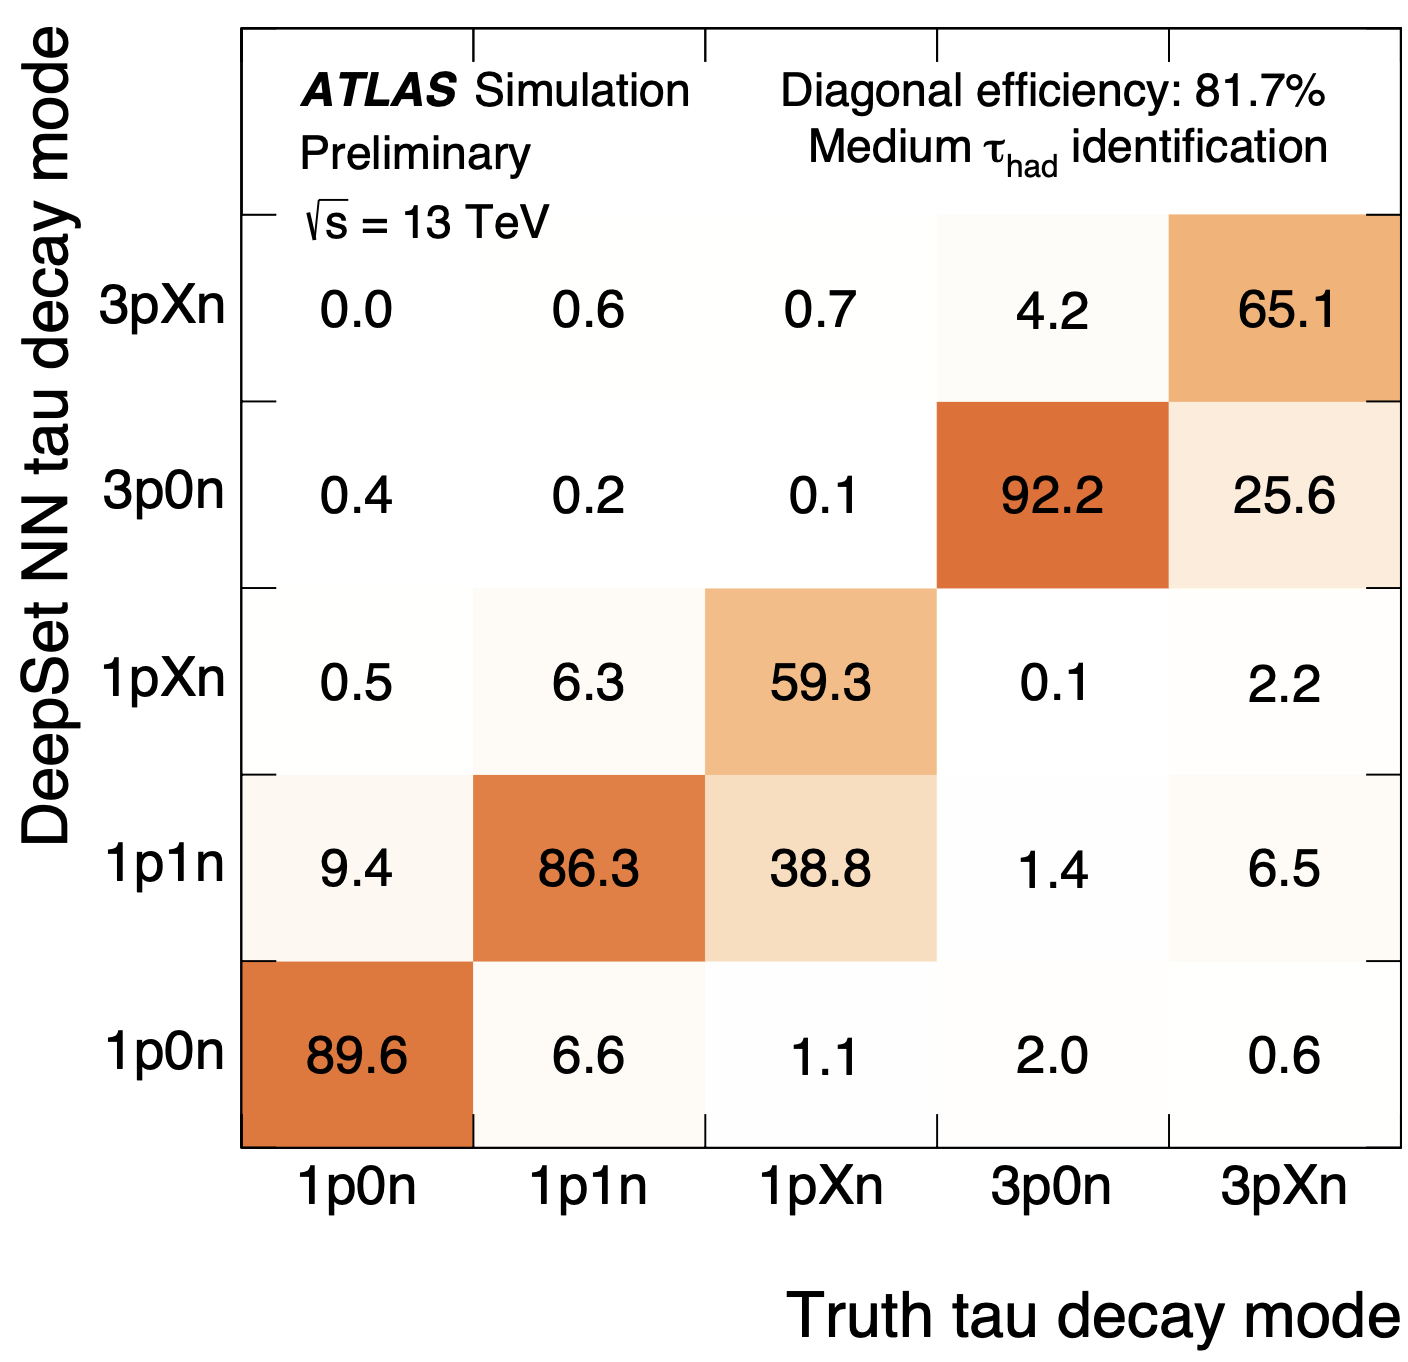
\includegraphics[width=0.45\textwidth]{decaymode_effi.png}
            \caption{
                Efficiency matrix for reconstructing the same $\tau$ lepton decay mode as the truth decay mode with DeepSet NN classifier 
                in $\gamma^*\rightarrow\tau\tau$ events, taken from~\cite{ATL-PHYS-PUB-2022-044}.
                The labels are in a form of `ApBn', where `A',`B' are the number of prongs (the `p') 
                and neutral pions (the `n') and `X' stands for more than one or more than zero accordingly.
            }
            \label{fig:tau_decay_mode_eff}
        \end{figure}

    \subsection{RNN-based electron-veto}
        Electrons can be misidentified as $\tauhadvis$ candidates. In some analyses, 
        electrons represent a significant background contribution even after the suppression of jet-related 
        backgrounds through kinematic, topological, and tau identification criteria. Despite the similarities 
        between electron signatures and 1-prong \(\tauhadvis\), there are distinctive properties 
        that can be exploited for discrimination.
        Electrons are highly relativistic particles that emit transition radiation when traversing the 
        radiator material surrounding the straws of the TRT detector. This property, along with the 
        shape of the calorimetric energy deposits in combination with the track information, provides 
        a basis for discriminating electrons from \(\tauhadvis\). The ATLAS overlap removal procedure
        ensures that identified electrons are not double-counted as $\tauhadvis$ candidates. However
        the electron identification is not perfect, and some electrons may fail the electron identification and
        still be misidentified as $\tauhadvis$.

        The BDT-based e-veto algorithm used during Run 2 has been replaced by a novel approach based on RNN. 
        The updated RNN e-veto  offers multiple 
        working points for different levels of discrimination.
        The e-veto algorithm is trained using simulated samples of signal and background candidates. The signal sample is 
        the same as that used for the TauID algorithm, while the background sample consists of reconstructed
        $\tauhadvis$ candidates from \(Z \rightarrow ee\) processes, required to pass the Medium 
        $\tauhadvis$ identification working point.
    
        Dedicated neural networks are trained separately for 1-prong and 3-prong $\tauhadvis$ cases. 
        The reconstructed \pT of the $\tauhadvis$ is used to re-weight the samples, ensuring 
        no \pT-dependent bias in the trained classifier. The training minimises the binary cross-entropy 
        loss function~\cite{mao2023crossentropylossfunctionstheoretical} using stochastic gradient descent (SGD)~\cite{ruder2016overview}
        with momentum and a step-wise reduction of the optimiser's learning rate.
    
        The e-veto algorithm's output score is transformed to provide a uniform efficiency with respect 
        to \pt and \(\eta\) of the true \(\tauhadvis\). The algorithm defines three working 
        points (Loose, Medium, Tight) for different levels of electron rejection efficiency.
        The performance of the e-veto algorithm is evaluated on independent test samples, measuring the 
        $\tauhadvis$ efficiency and electron rejection factor as functions of $\langle \mu \rangle$ and the \pt of 
        1-prong and 3-prong $\tauhadvis$ candidates.
        Figure \ref{fig:eveto_eff} shows the rejection for misidentified 1-prong and 3-prong $\tauhadvis$ candidates from $Z\rightarrow ee$
        background events as a function of the efficiency for truth $\tauhad$ originating from $\gamma^*\rightarrow\tau\tau$ events.
        \begin{figure}[htbp]
            \centering
            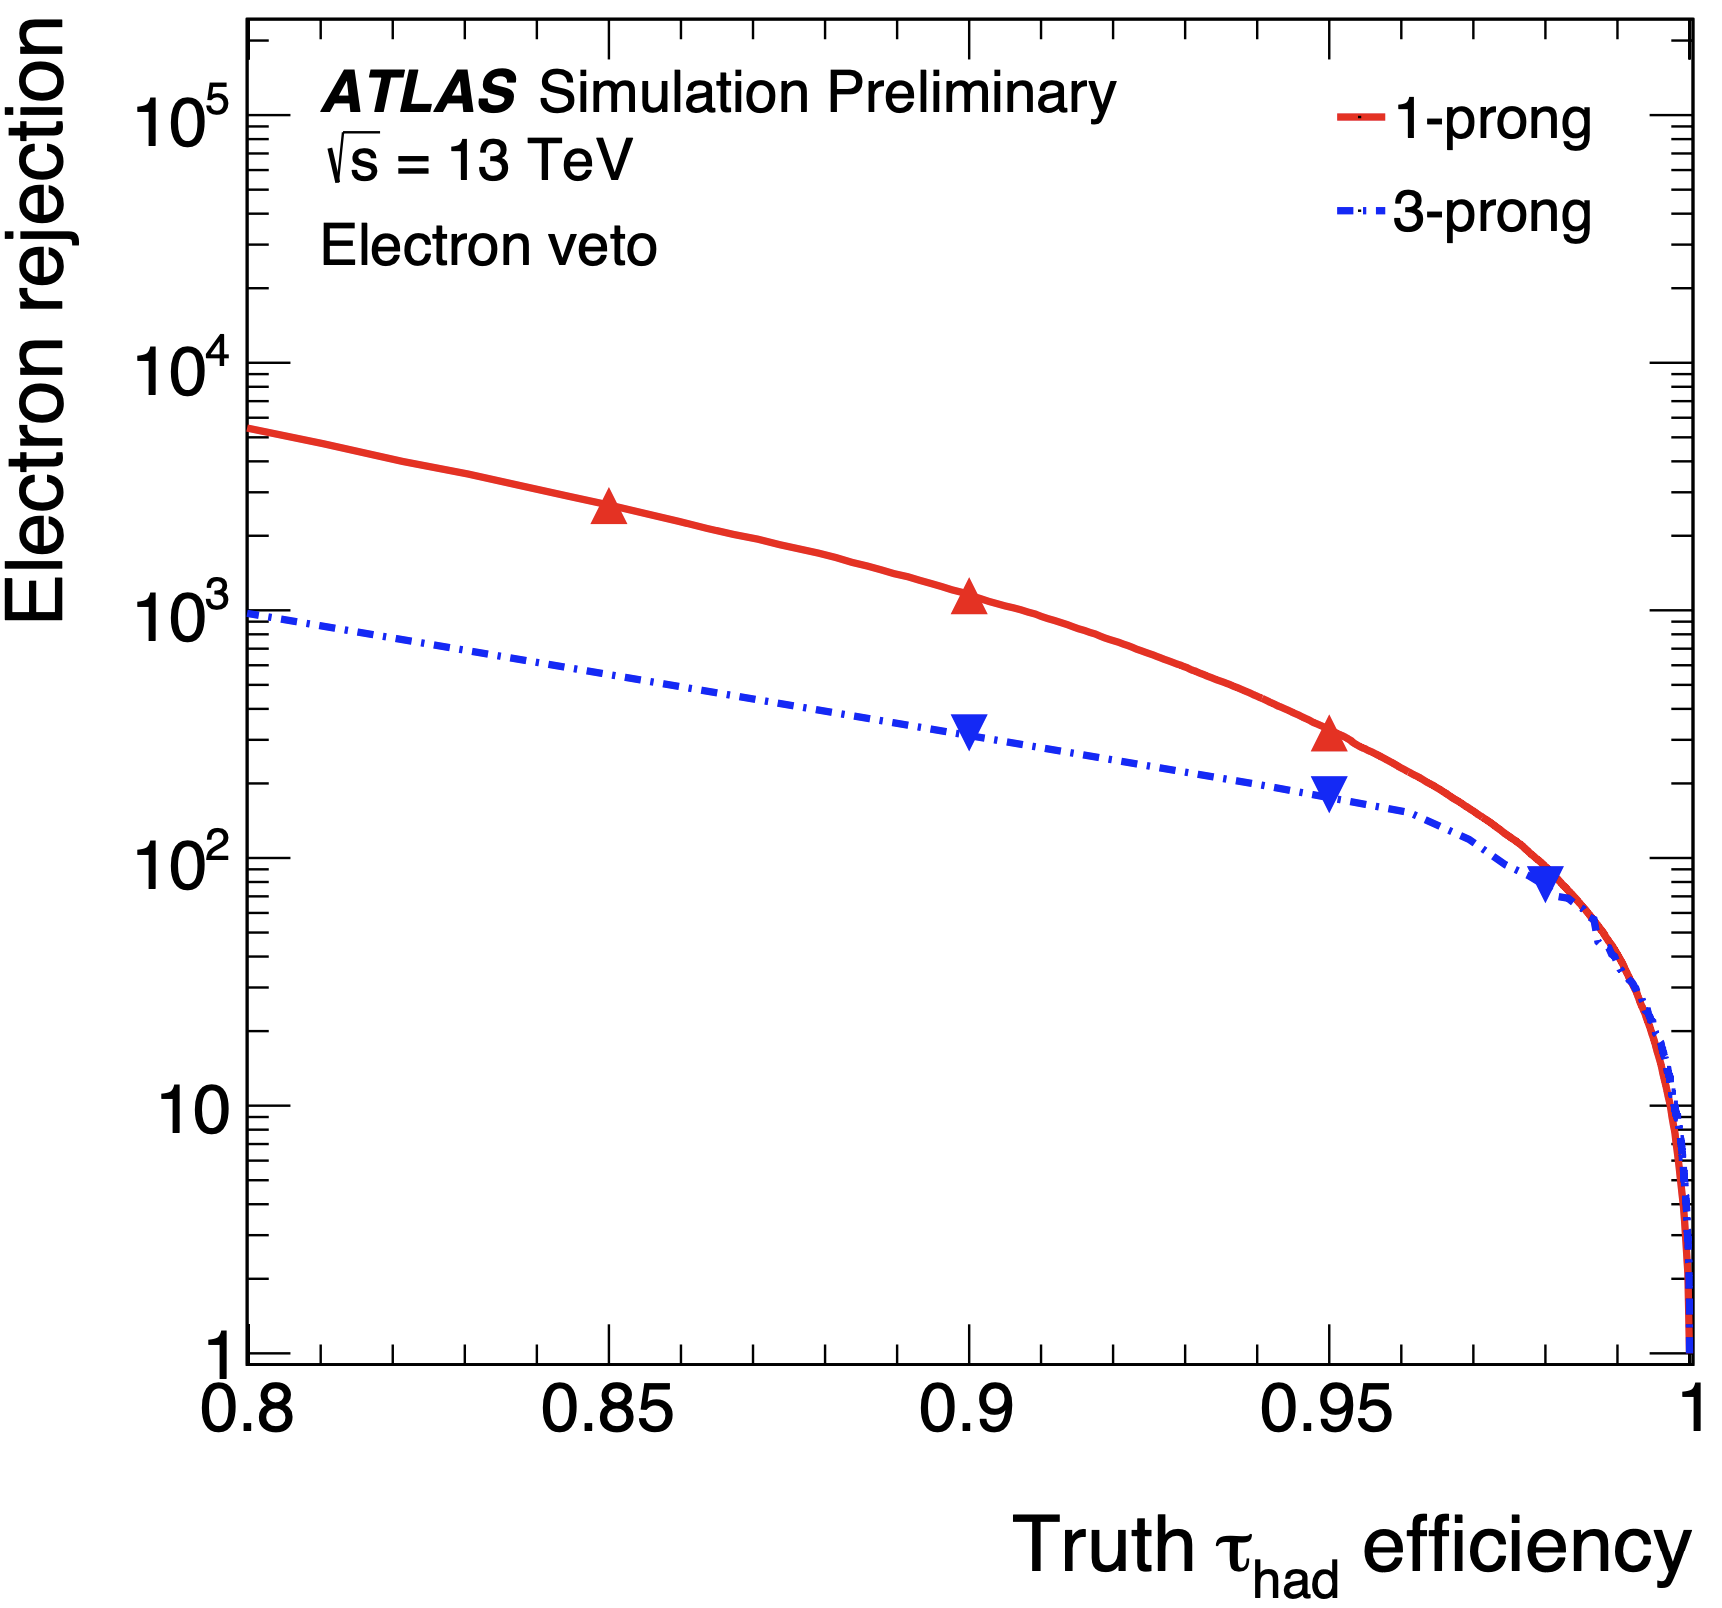
\includegraphics[width=0.45\textwidth]{eveto_roc.png}
            \caption{
                Rejection for misidentified 1-prong and 3-prong $\tauhadvis$ candidates from $Z\rightarrow ee$
                background events with the e-veto algorithm,
                as a function of the efficiency for truth $\tauhad$ originating from $\gamma^*\rightarrow\tau\tau$ events, taken from~\cite{ATL-PHYS-PUB-2022-044}.
            }
            \label{fig:eveto_eff}
        \end{figure}

\section{$\tauhadvis$ Energy calibration and resolution}
    The energy calibration of $\tauhad$ involves several steps to ensure accurate 
    measurement of the visible energy.
    \begin{itemize}
        \item Pre-calibration: initial energy estimates are obtained from the seed jets.
        \item MC-based corrections: corrections derived from MC simulations are applied to account for detector response and other systematic effects.
        \item Boosted regression tree (BRT) refinement: the boosted regression tree algorithm refines the energy estimates using additional input variables and sequential data from the RNNs.
        \item Data-driven corrections: final adjustments are made using data-driven techniques, comparing MC predictions with actual data to ensure consistency and accuracy.
    \end{itemize}

    \subsubsection{Pre-calibration}
        Pre-calibration is the initial step in the energy calibration process for $\tauhadvis$. 
        This step involves obtaining preliminary energy estimates from the visible decay products of the 
        tau leptons, utilising data from the calorimeter and tracking systems of the detector. After the 
        reconstruction of $\tauhadvis$ candidates, the four-momentum of the $\tauhadvis$
        candidate is calculated by summing the momenta of all associated clusters and tracks. 
        This preliminary four-momentum estimate provides the initial energy scale for the tau candidates.

    \subsubsection{MC-based corrections}
        The MC-based corrections are derived from detailed simulations that model the interactions of 
        particles within the detector, accounting for various physical processes and detector effects. 
        The goal of MC-based corrections is to adjust the initial energy estimates obtained during 
        pre-calibration to more accurately reflect the true energy of the tau leptons.
        
        The energy scale correction adjusts the measured energy to account for systematic biases in the 
        calorimeter and tracking systems. This ensures that the average measured energy matches the true 
        energy over a wide range of tau energies. The resolution correction accounts for the smearing of 
        the energy measurement due to detector resolution effects. It ensures that the distribution of 
        measured energies around the true energy is correctly modelled.
        
        The MC-based corrections are derived by comparing the true energy of tau leptons in the simulation
        with the energy measured by the detector. This comparison is done as a function of key variables
        like $\pT$, $|\eta|$, and decay mode. The derived correction factors are applied to the initial 
        energy estimates of $\tauhad$ candidates. The corrected energy measurements are validated 
        by comparing key distributions (e.g., invariant mass of tau pairs) in data and simulation.

    \subsubsection{BRT refinement}
        BRT refinement is a sophisticated technique used to enhance the accuracy and precision of the 
        energy estimates of $\tauhad$. This method applies machine learning to correct residual 
        biases and improve the resolution of the energy measurements beyond what is achieved by MC-based 
        corrections alone.

        At the core of BRT are decision trees, which are simple predictive models that split data into 
        subsets based on feature values. Each split is chosen to minimise the error in predicting the 
        target variable, in this case, the tau energy. Boosting is an ensemble technique that combines 
        the predictions of multiple weak learners (individual decision trees) to form a stronger predictive 
        model. Trees are built sequentially, with each tree correcting the errors of its predecessors.
    
        The energy estimates obtained from pre-calibration and MC-based corrections
        serve as the starting point for BRT refinement. The BRT model is trained using the simulated 
        samples, where the input features (calorimeter and tracking variables) are used to predict 
        the true tau energy. The model learns to correct systematic biases and improve the precision 
        of the energy estimates. Once trained, the BRT model is applied to the actual data. The model 
        takes the MC-based energy estimates and the same set of input features to produce refined 
        energy predictions for $\tauhadvis$ candidates. The performance of the BRT refinement 
        is validated using independent test samples. Key metrics such as the energy resolution and 
        scale are evaluated to ensure the model's predictions are accurate and unbiased.

    \subsubsection{Data-driven corrections}
        The data-driven method is the final step in the calibration process for $\tauhad$. 
        It involves using actual collision data to further refine and validate the energy calibration 
        obtained from MC-based corrections and BRT refinement. This approach helps to correct any 
        discrepancies between simulation and real data, ensuring that the final energy measurements 
        are as accurate and unbiased as possible~\cite{ATLAS-CONF-2017-029}.

        The data-driven method relies on reference processes to calibrate the
        energy measurements of $\tauhadvis$ candidates. Reference processes, such as
        well-understood physics decays like $\Zttmuhad$ are used as benchmarks to compare data and simulation. 
        The method exploits the fact that the distribution of the reconstructed visible mass of the $\tauhadvis$ and muon system, $m_\mathrm{vis}$, 
        in $\Zttmuhad$ events is sensitive to the differences in energy scale of the $\tauhadvis$ candidates between data and simulation.

        The $\tau$ energy scale (TES) correction is parameterised as $\pt\rightarrow(1+\alpha)\pt$ for $\tauhadvis$ candidates, where $\alpha$ is the TES correction factor.
        The muon energy scale is measured with high precision with independent methods. In Run 2, the TES correction factor is determined
        by minimising the difference between the $m_\mathrm{vis}$ distribution in data and simulation. Specifically, $\alpha$ is determined by minimising 
        $$\chi^2(\alpha, f) = \sum_i\frac{(N_i^\mathrm{data} - fN_i^\mathrm{sig}(\alpha) - N_i^\mathrm{bkg})^2}{N_i^\mathrm{data} + f^2(\Delta N_i^\mathrm{sig}(\alpha))^2+(\Delta N_i^\mathrm{bkg})^2},$$
        where $N_i^\mathrm{data/sig/bkg}$ is the number of events in the $i$-th bin of the $m_\mathrm{vis}$ distribution in data, signal, or background; 
        $\Delta N_i^\mathrm{sig}$ is the uncertainty in the number of signal events in the $i$-th bin; 
        and $f$ is a normalisation factor that accounts for the difference in the total number of events between data and simulation.
        
    %!TEX root = ../thesis.tex
%*******************************************************************************
%****************************** Third Chapter **********************************
%*******************************************************************************
\chapter{The muon-removal method for boosted \tmth reconstruction}

\graphicspath{{1_MainChapters/Chap5_MuonRM/fig}}


\section{Introduction} \label{sec:intro}
    % The $\tau$ lepton is the heaviest known lepton, with an invariant mass of 1.777~$\GeV$, and lifetime of $2.9\times10^{-13}\text{ s}$~\cite{RevPartPhys}. 
    % It has a 35\% probability of decaying leptonically to a lighter lepton (electron, $\taue$ or muon, $\taumu$; collectively referred to as $\taulep$) 
    % and two neutrinos. In the remaining 65\% of cases, the $\tau$ lepton decays hadronically ($\tauhad$) 
    % to one or more charged hadrons and zero or more neutral hadrons, plus one neutrino. Thus, the branching 
    % ratio for a pair of $\tau$ leptons to decay in the $\tau_\mathrm{lep}\tau_\mathrm{had}$ channel is 46\%. 

    % In the standard ATLAS $\tauhad$ reconstruction algorithm~\cite{ATLAS-CONF-2017-029, ATLAS-CONF-2011-152, ATL-PHYS-PUB-2019-033}, 
    % the reconstruction of the visible decay products of $\tauhad$ (\tauhadvis) is seeded by a jet clustered by the anti-\(k_{t}\) 
    % algorithm~\cite{Cacciari:2008gp} with a radius parameter of 0.4. The jet reconstruction algorithm operates on the 
    % calibrated~\cite{LocalHadronicCali}, clustered topological calorimeter cells~\cite{PERF-2014-07}. 
    % This seed jet is denoted as $\tauseed$. Only $\tauseed$ jets with transverse momentum $\pT > 5~\GeV$ and $|\eta| < 2.5$ are retained. 
    % The production vertex of the $\tauhad$ candidate is determined by the tau jet vertex association
    % algorithm~\cite{ATL-PHYS-PUB-2019-033}.
    % The inner detector tracks associated with the $\tauseed$ jet that originated from $\tauhad$ decay are selected by 
    % the track classification algorithm~\cite{ATL-PHYS-PUB-2019-033}.
    % The resulting $\tauhad$ candidate is then calibrated by the tau energy scale algorithms~\cite{ATL-PHYS-PUB-2019-033}.
    % After the reconstruction, the $\tauhad$ candidate is classified by the $\tauhad$ identification algorithm (TauID), 
    % a recurrent neural network (RNN) classifier~\cite{ATL-PHYS-PUB-2019-033}, to determine its likelihood of being the decay product of a $\tauhad$. 
    % A working point, ``Tight'', ``Medium'', ``Loose'' or ``VeryLoose'', is then assigned based on the signal efficiencies 
    % observed when tuning the RNN. The corresponding signal efficiencies for the $\tauhad$ identification working points
    % can be found in~\cite{ATL-PHYS-PUB-2019-033}.

    The standard ATLAS TauID algorithm is efficient unless activity from other particles is found inside the $\tauseed$ jet. 
    One of these cases is when a pair of $\tau$ leptons originates from a highly boosted resonance and the decay 
    products of the two $\tau$ leptons are reconstructed within the radius of a single $\tauseed$ jet. The 
    reconstruction and identification of boosted systems in which both $\tau$ leptons decay hadronically is 
    achieved by searching for hadronic $\tau\text{-like}$ substructure using a boosted decision tree within 
    a large radius seed jet~\cite{ATLAS-CONF-2020-012}. In this chapter, the decay in the $\tmth$ final state is considered.

    The minimum ionising nature of the muon and the fact that the muon reconstruction is independent of its isolation~\cite{MUON-2018-03} 
    prompt the idea of removing the track and clusters produced by the muon from the $\tauseed$ jet produced by a boosted $\tmth$ system. The 
    kinematic variables that are subsequently supplied to the TauID algorithm are re-calculated without the interference of 
    the muon. 
    %This approach recovers the signal efficiency in the $\tmth$ case nearly completely. 
    The $\tauhad$ reconstructed with this method is denoted as $\tauhadmurm$.

    The $\tauhadmurm$ method was developed using Monte Carlo (MC) simulated events corresponding to the beyond the standard model (BSM), 
    high-mass Graviton~\cite{Graviton_theory} decaying into two Higgs boson process as signal. However, before using this technique in future searches for 
    BSM physics, it is important to demonstrate its performance considering a standard model process. As a benchmark 
    for the new method, the production of two $\tau$ leptons originating from a highly boosted $Z$ boson decay is used. This process is 
    denoted as $\Zttmuhad$.\
    
    This chapter is organised as follows. 
    The data and MC samples are described in Section~\ref{sec:DataAndMCs}. 
    The development of the boosted $\tauhadmurm$ method is described in Section~\ref{sec:murm}. 
    The analysis methods for the $\Zttmuhad$ benchmark are described in Section~\ref{sec:Zttbench}. 
    The results of the $\Zttmuhad$ benchmark analysis are described in Section~\ref{sec:results}. 
    The summary and conclusions are given in Section~\ref{sec:conclusion}.



\section{Data and simulated samples} \label{sec:DataAndMCs}
    \subsection{Simulated samples for development of the method} \label{sec:DevelopmentMC}
        MC simulated event samples are used to model the signal and the background to develop 
        the $\tauhadmurm$ method and  to evaluate  the $\tau$ identification efficiency
        and background rejection power. The signal sample consists of BSM Gravitons~\cite{Graviton_theory} 
        decaying to a pair of Higgs bosons, with the hypothetical Graviton mass ranging from 
        1000~$\GeV$ to 5000~$\GeV$. To maximise the signal statistics, the Higgs boson is constrained to decay to 
        a pair of $\tau$ leptons. The signal process is denoted by $\GHHFourtau$. 

        A high-\pT, semi-leptonically decaying heavy flavour hadron may produce a detector signature that has some similarities with 
        the signal sample of boosted $\tmth$ pair systems, since the invariant mass of the charmed hadron produced in the 
        semi-leptonic decay of a B hadron is comparable to that of the $\tau$ lepton. 
        The $\ttbar$ process is used to model this type of background.

        The $\GHHFourtau$ signal samples are generated using the \textsc{MadGraph 5}~\cite{Alwall:2014hca} matrix element (ME) generator. 
        The production of \ttbar events is modelled using the
        \POWHEGBOX[v2]~\cite{Frixione:2007nw,Nason:2004rx,Frixione:2007vw,Alioli:2010xd}
        generator at NLO with the \NNPDF[3.0nlo]~\cite{Ball:2014uwa} PDF set
        and the \hdamp parameter\footnote{The
        \hdamp parameter is a resummation damping factor and one of the
        parameters that controls the matching of \POWHEG matrix elements to
        the parton shower and thus effectively regulates the
        high-\pT radiation against which the \ttbar system recoils.} set
        to 1.5~\mtop ~\cite{ATL-PHYS-PUB-2016-020}.

        \PYTHIA~\cite{Sjostrand:2014zea} with the A14~\cite{ATL-PHYS-PUB-2014-021} tuned parameters and \NNPDF[2.3lo]~\cite{Ball:2012cx} 
        PDF is used for the simulation of the parton showering and hadronisation for both the $\GHHFourtau$ samples and
        the \ttbar samples. The decays of bottom and charm hadrons were performed by \EVTGEN[1.6.0]~\cite{Lange:2001uf}.
        The effect of multiple interactions in the same and neighbouring bunch crossings (pile-up) was modelled
        by overlaying the original hard-scattering
        event with simulated inelastic events generated by
        \PYTHIA[8.186]~\cite{Sjostrand:2014zea} with the A3 tune~\cite{ATL-PHYS-PUB-2016-017} 
        and the MSTW2008LO PDF set~\cite{Martin:2009iq}.
        The MC samples were re-weighted so that the pile-up distribution matches the one observed in the data.
        All MC samples are passed  through the 
        ATLAS detector simulation based on \textsc{Geant 4}~\cite{Agostinelli:2002hh}. 

    \subsection{Data and simulated samples for the benchmark analysis} \label{sec:Benchmark}
        For the $\Zttmuhad$ benchmark analysis, the full Run 2 dataset collected in $pp$ collisions at the LHC~\cite{Evans:2008zzb} with a centre-of-mass
        energy of 13~$\TeV$ and a 25~ns bunch crossing interval is utilised. The integrated luminosity of the dataset recorded
        while all relevant components of the ATLAS detector were operated in their nominal operating
        conditions  corresponds to 140~\ifb~\cite{DAPR-2021-01}. 

        Simulated samples provide predictions for both signal and background processes.
        As in Section~\ref{sec:DevelopmentMC},
        the simulation includes the effect of multiple \(pp\) interactions per bunch crossing, as well as the impact on the detector response due to
        interactions from bunch crossings before or after the one containing the hard interaction. 
        All MC samples undergo detector simulation, calibration, and corrections to match the performance in data. 
        For all simulated samples, the next-to-next-to-leading-order (NNLO) PDF is employed for ME calculations.
        The decays of bottom and charm hadrons
        were performed by \EVTGEN~\cite{Lange:2001uf}.
        The rest of this section gives details of the specific MC samples used in this study.

        The dominant production channel of the boosted $\Zttmuhad$ final state, 
        a $Z$ boson produced in association with jets was modelled using the
        \SHERPA[2.2.14]~\cite{Bothmann:2019yzt} MC generator in the $\Ztautau$ channel;
        while the \SHERPA[2.2.11] MC generator was used in the $Z\rightarrow ll~(l=e,\mu)$ channels.
        The ME calculations range from next-to-leading order (NLO) for final 
        states with up to two additional parton emissions to leading order 
        (LO) for up to five additional parton emissions. 
        The matrix elements were merged with the \SHERPA parton shower following the \MEPSatLO~\cite{Hoeche:2009rj} prescription and using the \NNPDF[3.0nnlo] set of PDFs~\cite{Ball:2014uwa}.
        The production of $W$ boson with jets, and the production of $WW, WZ$, and $ZZ$ boson pairs, was simulated with the \SHERPA[2.2.11] with similar configurations as the $Z$+jets sample.
        For $Z$ boson production, particularly for events with $\pt^{Z} > 100~\GeV$, comparing with the measurements of $Z$-boson $p_T^{Z}$ 
        and $\phi^*_\eta$ using light-lepton pair events at 13~TeV~\cite{STDM-2018-14},
        the cross-section for $Z$ boson events with high $\pt^{Z}$ modelled by \SHERPA[2.2.11] is 
        approximately 10\% lower than in data~\cite{PMGR-2021-01}. The simulation of initial state QCD 
        radiation is expected to be similar in the \SHERPA[2.2.14] sample used in this study. A 10\% 
        correction is applied to the predicted numbers for 
        $\Ztautau$ events, with the full size of this correction quoted as a systematic uncertainty.


        The production of \ttbar events was modelled using the same configuration as the one used for the method development.

        Single-top \(t\)-channel production was modelled using the
        \POWHEGBOX[v2]~\cite{Frederix:2012dh,Nason:2004rx,Frixione:2007vw,Alioli:2010xd}
        generator at NLO in QCD using the four-flavour scheme and the
        corresponding \NNPDF[3.0nlo] set of PDFs~\cite{Ball:2014uwa}.  The events were
        interfaced with \PYTHIA[8.230]~\cite{Sjostrand:2014zea} using the A14
        tune~\cite{ATL-PHYS-PUB-2014-021} and the \NNPDF[2.3lo] set of
        PDFs~\cite{Ball:2012cx}.

        The associated production of top quarks with \(W\) bosons (\(tW\)) was
        modelled by the
        \POWHEGBOX[v2]~\cite{Re:2010bp,Nason:2004rx,Frixione:2007vw,Alioli:2010xd}
        generator at NLO in QCD using the five-flavour scheme and the
        \NNPDF[3.0nlo] set of PDFs~\cite{Ball:2014uwa}.
        The diagram removal scheme~\cite{Frixione:2008yi} was used to
        remove interference and overlap with \ttbar production.
        The events were interfaced to \PYTHIA[8.230]~\cite{Sjostrand:2014zea} using the A14
        tune~\cite{ATL-PHYS-PUB-2014-021} and the \NNPDF[2.3lo] set of
        PDFs~\cite{Ball:2012cx}.

\section{Development of the boosted $\tauhadmurm$ reconstruction method} \label{sec:murm}
    \subsection{Muon removal and re-reconstruction of tau lepton candidate} \label{sec:muon_removal}
        The proximity between the $\tauhadvis$ and the muon 
        is represented by $\dRtttruthvis$, the $\Delta R$ between the MC 
        truth-level visible decay products of the two $\tau$ leptons. 
        In Figure~\ref{fig:murm:dr}, the $\dRtttruthvis$ distributions of the 
        \tmth pairs in the \GHHFourtau samples are presented.
        \begin{figure}[hbtp]
            \begin{center}
                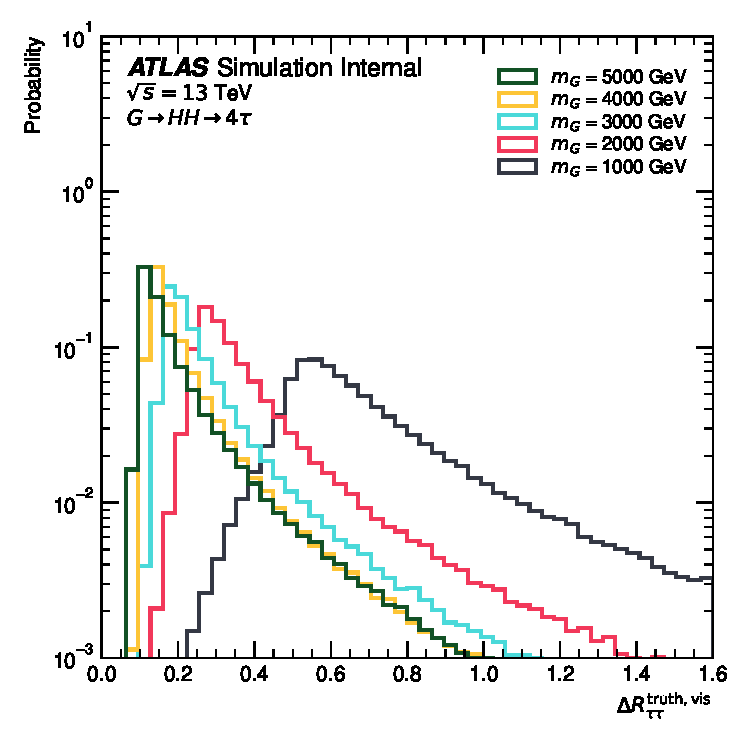
\includegraphics[width=0.50\textwidth]{plots_dev_fin/truth_dR_tt.pdf}
                \caption{The distributions of the $\dRtttruthvis$ between the truth 
                    level \tmth pair in the \GHHFourtau with hypothetical Graviton 
                    mass ranging from 1000 GeV to 5000 GeV. The distributions are normalised to unity.}
                \label{fig:murm:dr}
            \end{center}
        \end{figure}
        If the $\dRtttruthvis < 0.4$, it is likely that the muon will 
        be reconstructed inside the $\tauseed$ jet. 
        %However, for $\dRtttruthvis > 0.4$, the muon is not expected to overlap with the $\tauseed$ jet.

        For the purposes of this study, MC truth information is used to match truth-level $\tmth$ pairs with 
        their reconstructed counterparts. This facilitates focusing on only $\tauseed$ jets originating 
        from the boosted $\tmth$ pair and allows other $\tauseed$ jets associated with QCD jets to be neglected. 
        The MC truth-level visible $\tau$ decay products are required to satisfy the 
        requirements $p_T > 20\text{ \GeV}$ and $|\eta| < 2.5$, to ensure that the $\tauseed$ jets 
        are within the tracking acceptance of the ATLAS detector. 

        \begin{figure}[hbtp]
            \begin{center}
                \subfloat[]{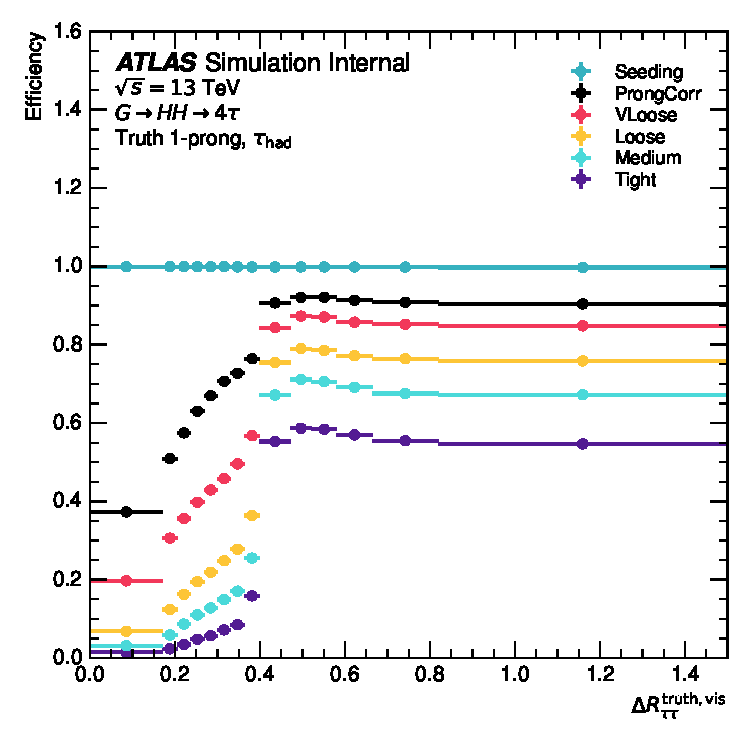
\includegraphics[width=0.5\textwidth]{plots_dev_fin/eff_nocut_dR_off_1p.pdf}\label{fig:murm:effi_off_1p}}
                \subfloat[]{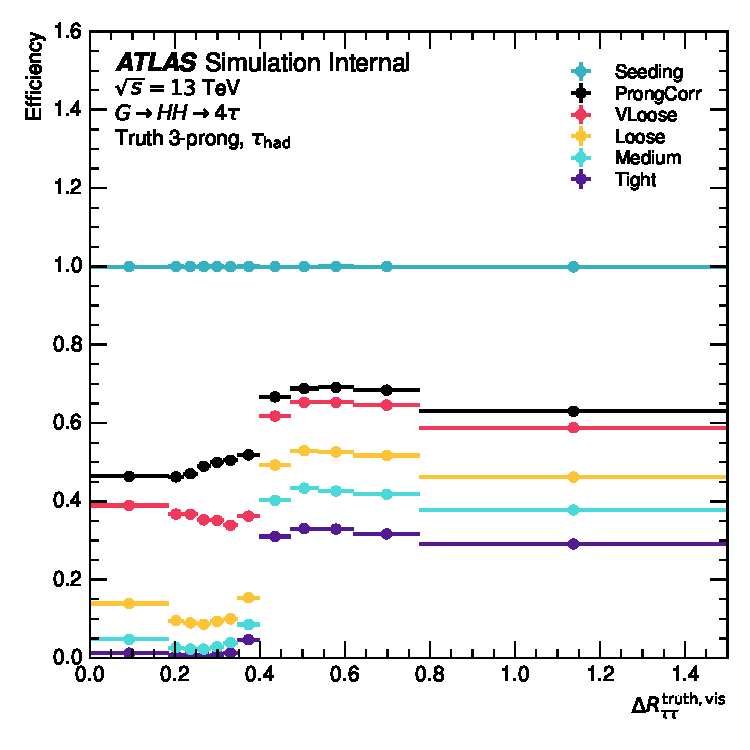
\includegraphics[width=0.5\textwidth]{plots_dev_fin/eff_nocut_dR_off_3p.pdf}\label{fig:murm:effi_off_3p}}
                \caption{The combined reconstruction and identification efficiencies of the standard ATLAS TauID for 
                    truth 1-prong~(\protect\subref{fig:murm:effi_off_1p}) and 3-prong~(\protect\subref{fig:murm:effi_off_3p}) $\tmth$ pairs 
                    in all working points as a function of $\dRtttruthvis$; the ``Seeding'' line 
                    (dark cyan) shows the efficiency of a $\tauseed$ jet that matches to a truth-level $\tmth$ pair being 
                    reconstructed; the ``ProngCorr'' line (black) shows the efficiency of a truth-level $\tauhad$ being 
                    reconstructed with the correct number of associated charged-particle tracks.
                }
                \label{fig:murm:effi_off}
            \end{center}
        \end{figure}

        The loss of performance of the standard TauID algorithm in the low $\dRtttruthvis$ 
        region is illustrated in Figure~\ref{fig:murm:effi_off}, which shows the combined reconstruction and identification efficiencies of 
        the standard ATLAS $\tauhad$ reconstruction algorithm and TauID algorithm as a function of $\dRtttruthvis$ for truth ``1-prong'' and ``3-prong'' 
        $\tmth$ pairs. Here the ``n-prong'' denotes the number of charged hadrons that originate from the $\tauhad$ decay. 
        The efficiency for a $\tauseed$ jet to be reconstructed from a truth-level $\tmth$ pair remains high for all 
        values of $\dRtttruthvis$. However, the efficiencies for all standard TauID working 
        points drop significantly in both ``1-prong'' and ``3-prong'' cases when $\dRtttruthvis < 0.4$. 
        The tighter the working point, the greater the fractional loss in efficiency due to the presence of the nearby
        muon. The performance of the standard TauID algorithm is set as a baseline in this study.

        The muon's nature as a minimum ionising particle, combined with the fact 
        that its reconstruction is independent of its isolation~\cite{MUON-2018-03}, 
        provides a motivation for excluding the inner detector track and calorimeter 
        clusters associated with any nearby muon from the the standard ATLAS $\tauhad$ reconstruction algorithm. 
        %Inclusion of their associated tracks and clusters could lead to contamination in the reconstruction of the $\tauseed$ jet. 
        By removing these contributions, the $\tauseed$ jet would better represent 
        only the hadronically decaying $\tau$, improving the accuracy of TauID.
        Specifically, the inner detector track and clusters associated with a reconstructed muon that 
        satisfies the ``Medium'' muon ID working point~\cite{MUON-2018-03} 
        is removed if the track or cluster is found within the reconstructed $\tauseed$ jet. 
        After the muon removal, the standard 
        hadronic tau reconstruction algorithm is re-run on the $\tauseed$ jet. In this way, the relevant ID variables for 
        the hadronically decaying $\tau$ can be calculated without the muon component.

    \subsection{Performance of the method} \label{sec:murm_perf}
        \begin{figure}[hbtp]
            \begin{center}
                \subfloat[]{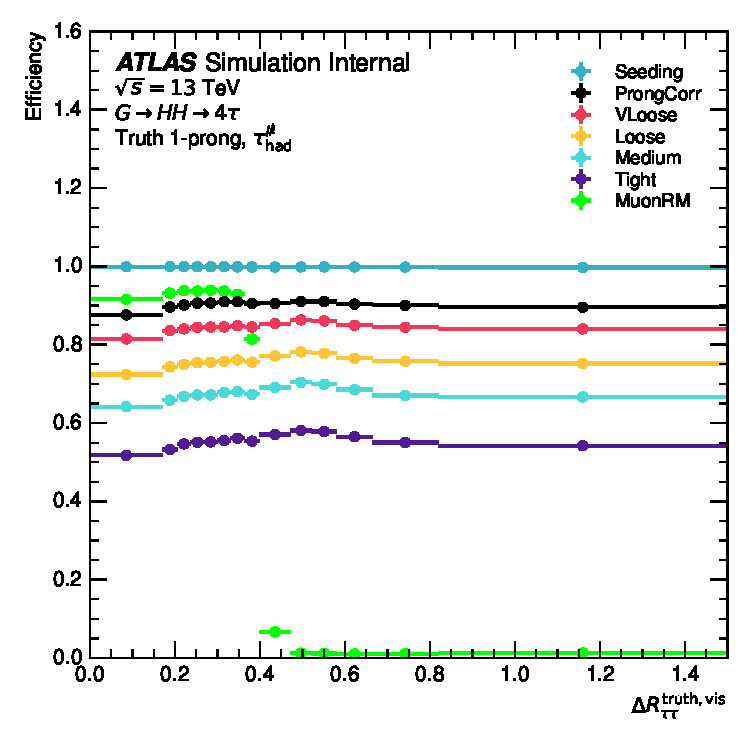
\includegraphics[width=0.5\textwidth]{plots_dev_fin/eff_nocut_dR_new_1p.pdf}\label{fig:murm:effi_new_1p}}
                \subfloat[]{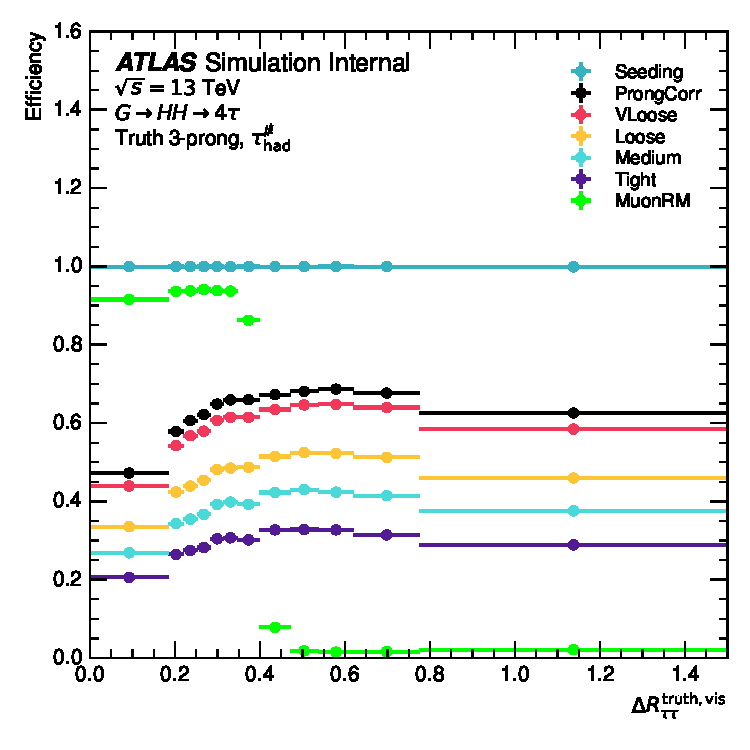
\includegraphics[width=0.5\textwidth]{plots_dev_fin/eff_nocut_dR_new_3p.pdf}\label{fig:murm:effi_new_3p}}
                \caption{The combined reconstruction and TauID efficiencies 
                    after the muon removal for truth 1-prong~(\protect\subref{fig:murm:effi_new_1p})
                    and 3-prong~(\protect\subref{fig:murm:effi_new_3p}) 
                    $\tmth$ pairs in all working points as a function of $\dRtttruthvis$. 
                    The extra ``MuonRM'' line (green) shows the efficiency of a muon 
                    being removed from the \tauseed. The slight abnormality in the ``MuonRM'' line 
                    between $0.35 < \dRtttruthvis < 0.45$ is due to limited detector 
                    resolution in the direction of the reconstructed $\tauhadvis$.
                }
                \label{fig:murm:effi_new}
            \end{center}
        \end{figure}
        Figure~\ref{fig:murm:effi_new} shows the combined reconstruction and identification efficiencies after muon removal as a function of 
        $\dRtttruthvis$ for truth 1-prong and 3-prong $\tmth$ pairs in all working points. 
        The reconstruction and identification efficiencies after muon removal show a considerable improvement compared to those shown 
        in Figure~\ref{fig:murm:effi_off}. The signal efficiency is recovered almost completely in every working point 
        for both 1-prong and 3-prong $\tauhad$. For 3-prong cases, the efficiency of TauID is limited by the 
        accurate reconstruction of the correct number of tracks associated with the highly boosted 
        $\tauhad$ (referred to as ``ProngCorr''). 
        % The performance metrics for the identification of 3-prong 
        % $\tauhad$ without incorporating the ``ProngCorr'' criterion are presented in the Appendix. 
        % A full recovery of the signal efficiency for the identification of 3-prong $\tauhad$.


        Roughly 95\% of the $\tauseed$ jets have a muon removed in the region where $\dRtttruthvis < 0.4$. 
        This can be expected given the 97\% efficiency of the ``Medium'' muon ID working point, 
        with a dip below 90\% in the region $\absetatruthvis < 0.1$. This is illustrated in 
        Figure~\ref{fig:murm:etaRM}, which shows the signal efficiencies of the TauID working points after muon removal as a 
        function of the $\absetatruthvis$ for truth 1-prong and 3-prong $\tauseed$ jets with 
        $\dRtttruthvis < 0.4$. 
        % The dip in efficiency for $\absetatruthvis < 0.1$ is caused by
        % the muon identification inefficiency for central muons.

        \begin{figure}[hbtp]
            \begin{center}
                \subfloat[]{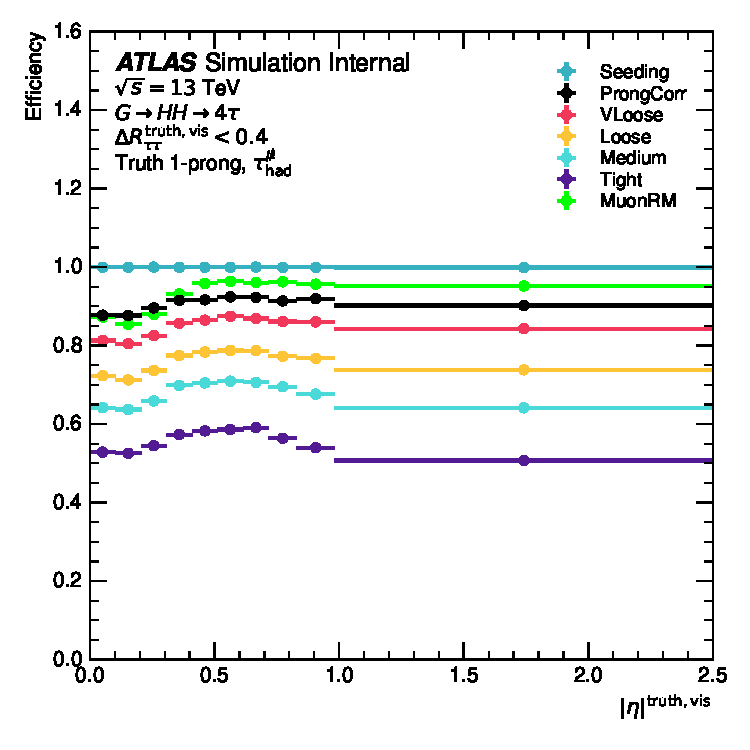
\includegraphics[width=0.50\textwidth]{plots_dev_fin/eff_dR04_eta_new_1p.pdf}\label{fig:murm:etaRM_1p}}
                \subfloat[]{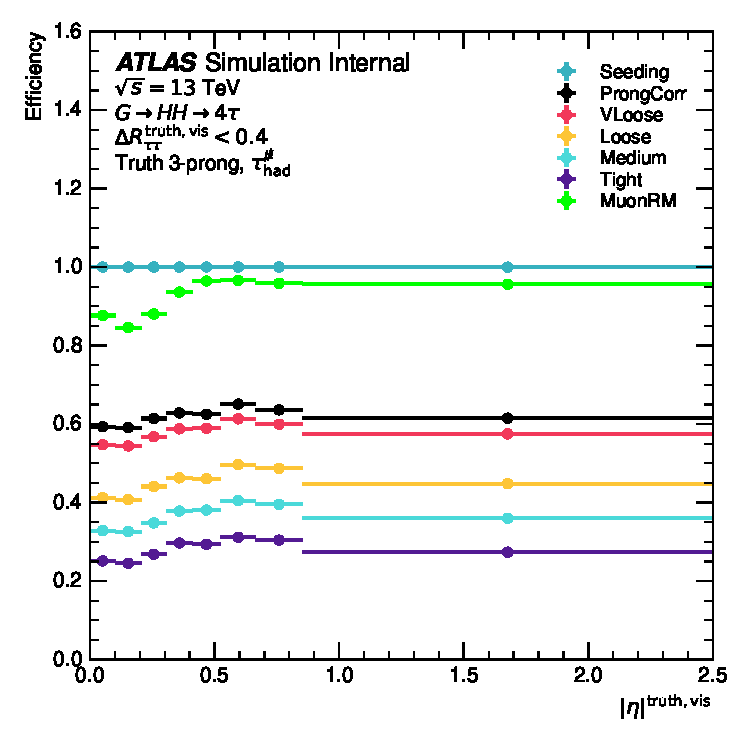
\includegraphics[width=0.50\textwidth]{plots_dev_fin/eff_dR04_eta_new_3p.pdf}\label{fig:murm:etaRM_3p}}
                \caption{The signal efficiencies of the TauID working points as a function of the truth absolute pseudorapidity 
                for truth 1-prong~(\protect\subref{fig:murm:etaRM_1p}) and 3-prong~(\protect\subref{fig:murm:etaRM_3p}) $\tauseed$ jets
                with $\dRtttruthvis < 0.4$. The seeding efficiencies and the ratio of the 
                $\tauseed$ jets with a muon removed are also shown.}
                \label{fig:murm:etaRM}
            \end{center}
        \end{figure}

        The signal identification efficiencies in all working points of the standard ATLAS TauID are tuned to show minimum 
        dependency on the $\pttautruthvis$ and pile-up~\cite{ATL-PHYS-PUB-2019-033}. The stability 
        of the TauID working point efficiencies after muon removal against these variables is shown in Figure~\ref{fig:murm:stability}. 
        To focus on the objects of interest, only truth $\tmth$ pairs with the $\Delta R$ between the reconstructed muon and $\tauhad$, $\dRttreco < 0.4$ 
        are included in the plots. For comparison, the TauID working point efficiencies as a function of the same variables 
        for $\tauseed$ objects in which muon removal is not required ($\dRtttruthvis > 0.45$) 
        are shown in Figure~\ref{fig:murm:45drstability}. Similar behaviour is observed in figures~\ref{fig:murm:stability} and~\ref{fig:murm:45drstability}. 
        The improved performance and good stabilities across different working points demonstrate that, after muon removal, 
        the TauID RNN sees the signal $\tauseed$ jet as if it were a $\tauhad$ that is free from interference of surrounding particles (isolated $\tauhad$).

        \begin{figure}[hbtp]
            \begin{center}
                \subfloat[]{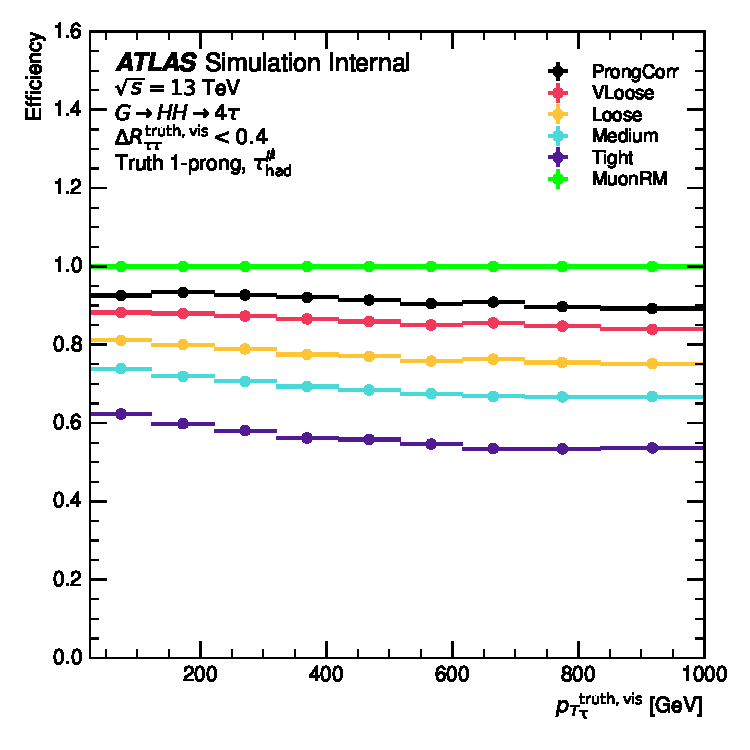
\includegraphics[width=0.50\textwidth]{plots_dev_fin/eff_dR04_murm_pt_new_1p.pdf} \label{fig:murm:ptDR04_1p}}  
                \subfloat[]{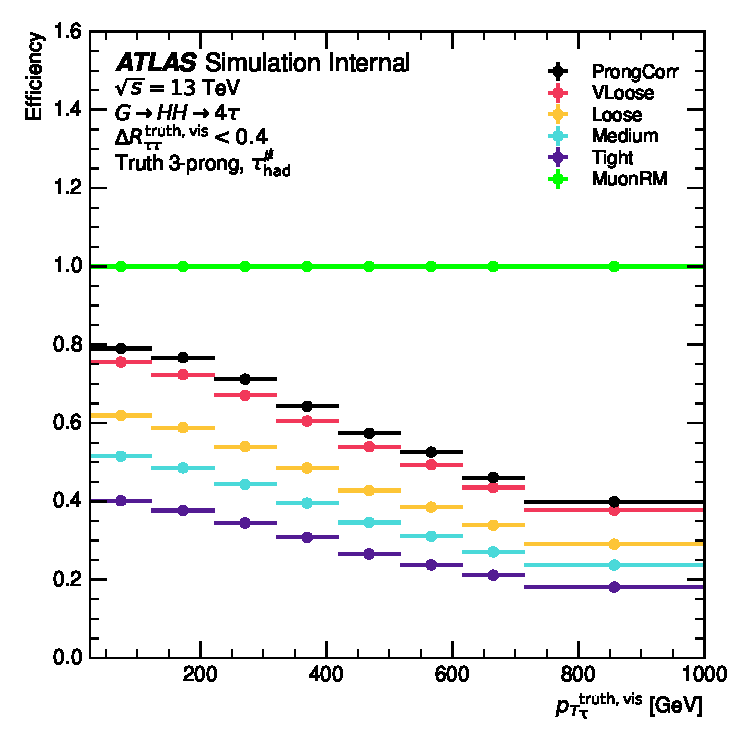
\includegraphics[width=0.50\textwidth]{plots_dev_fin/eff_dR04_murm_pt_new_3p.pdf} \label{fig:murm:ptDR04_3p}}  
                \vspace{-0.45cm} % Adjust the negative space here to bring rows closer
                \\
                % \subfloat[]{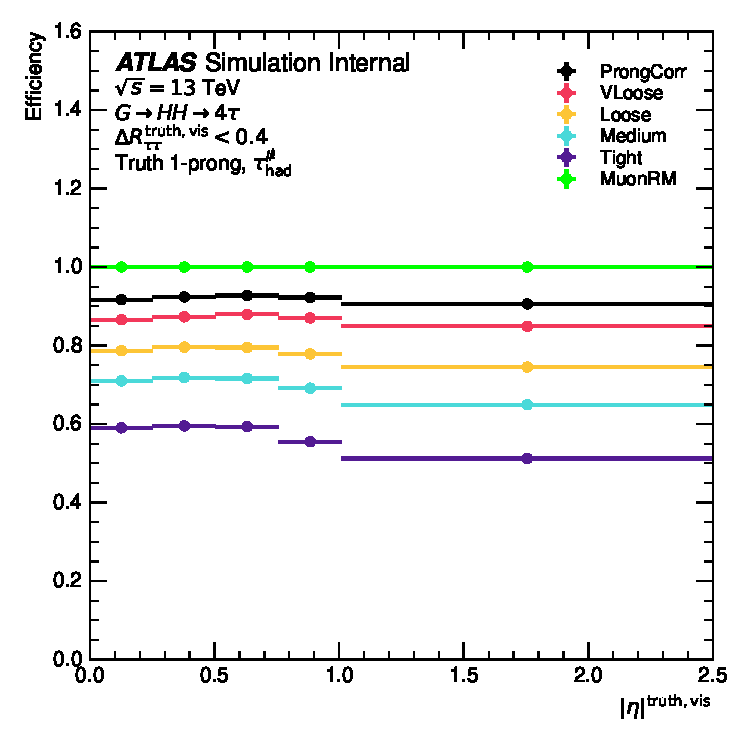
\includegraphics[width=0.50\textwidth]{plots_dev_fin/eff_dR04_murm_eta_new_1p.pdf}\label{fig:murm:etaDR04_1p}}
                % \subfloat[]{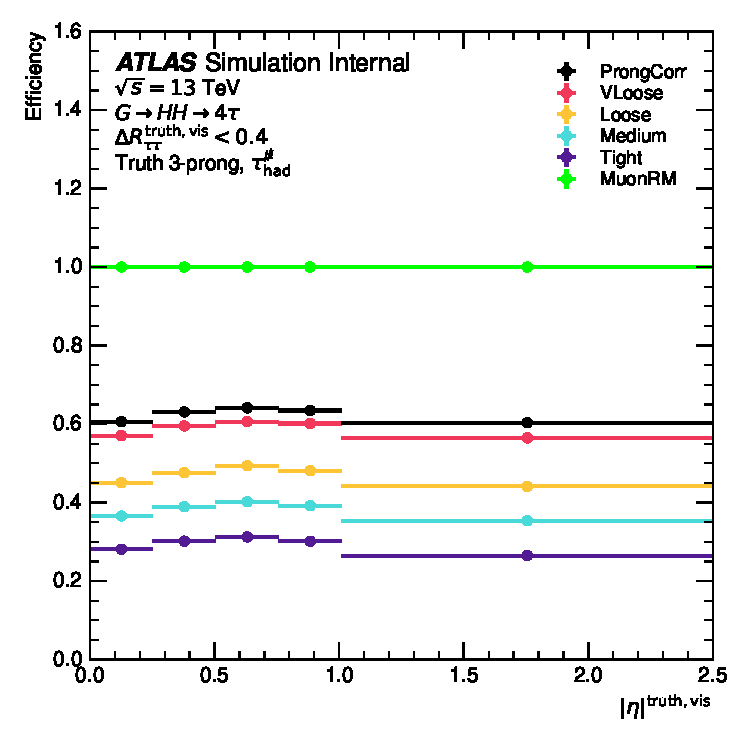
\includegraphics[width=0.50\textwidth]{plots_dev_fin/eff_dR04_murm_eta_new_3p.pdf}\label{fig:murm:etaDR04_3p}}
                % \vspace{-0.45cm} % Adjust the negative space here to bring rows closer
                % \\
                \subfloat[]{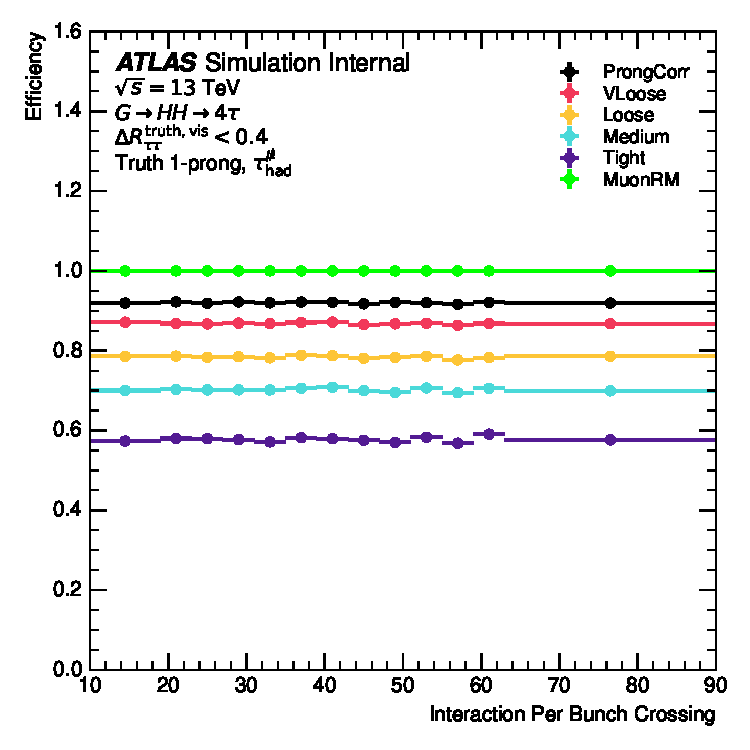
\includegraphics[width=0.50\textwidth]{plots_dev_fin/eff_dR04_murm_mu_new_1p.pdf} \label{fig:murm:muDR04_1p}}  
                \subfloat[]{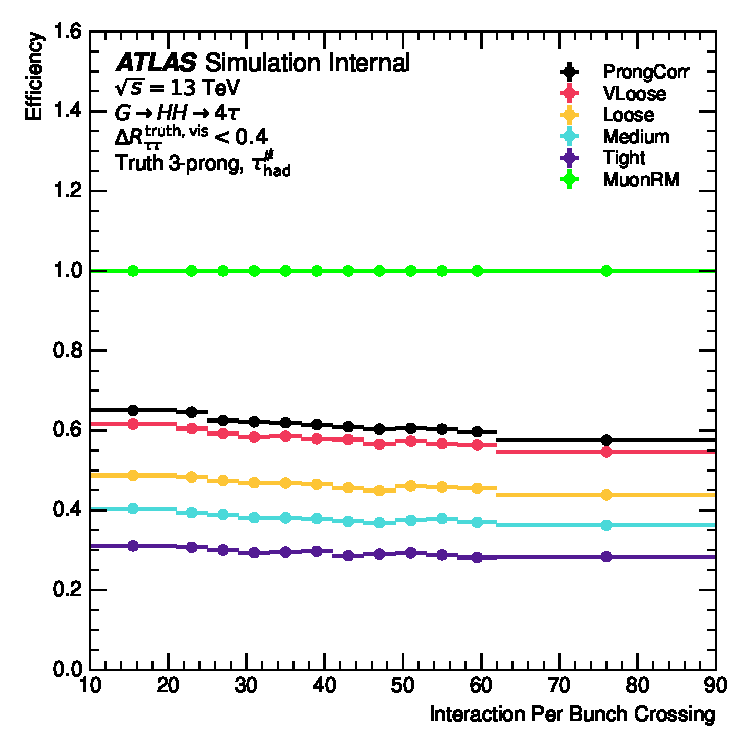
\includegraphics[width=0.50\textwidth]{plots_dev_fin/eff_dR04_murm_mu_new_3p.pdf} \label{fig:murm:muDR04_3p}}  
                \caption{The stability of the signal efficiencies of the TauID working points against 
                    the truth transverse momentum~(\protect\subref{fig:murm:ptDR04_1p})~(\protect\subref{fig:murm:ptDR04_3p}), 
                    % absolute pseudorapidity~(\protect\subref{fig:murm:etaDR04_1p})~(\protect\subref{fig:murm:etaDR04_3p}), 
                    and pile-up~(\protect\subref{fig:murm:muDR04_1p})~(\protect\subref{fig:murm:muDR04_3p}) for truth 
                    1-prong and 3-prong $\tauseed$ with reconstructed $\dRttreco < 0.4$.
                    The ``Seeding'' lines indicate the efficiency 
                    of a truth-level $\tauhad$ being reconstructed as $\tauseed$. The ``MuonRM'' lines show the efficiency of 
                    a muon being removed inside the $\tauseed$.
                }
                \label{fig:murm:stability}
            \end{center}
        \end{figure}

        \begin{figure}[hbtp]
            \begin{center}
                \subfloat[]{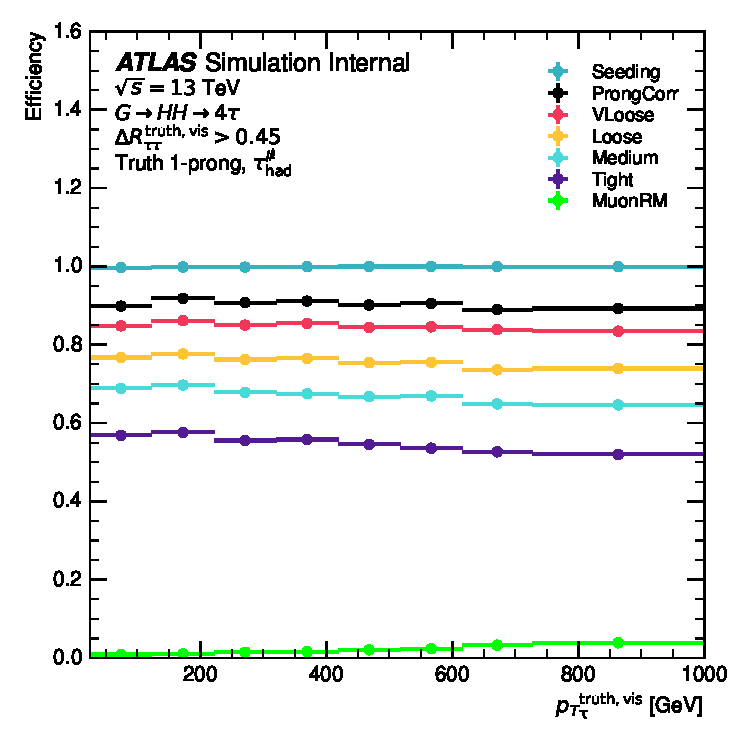
\includegraphics[width=0.50\textwidth]{plots_dev_fin/eff_04dR_pt_new_1p.pdf}  \label{fig:murm:pt45dr_1p}}
                \subfloat[]{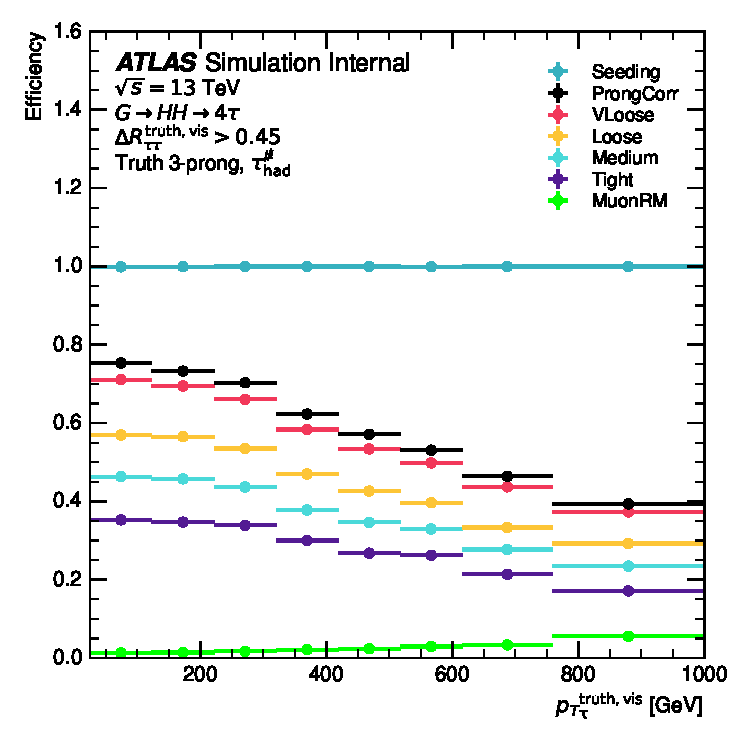
\includegraphics[width=0.50\textwidth]{plots_dev_fin/eff_04dR_pt_new_3p.pdf}  \label{fig:murm:pt45dr_3p}}
                \vspace{-0.45cm} % Adjust the negative space here to bring rows closer
                \\
                % \subfloat[]{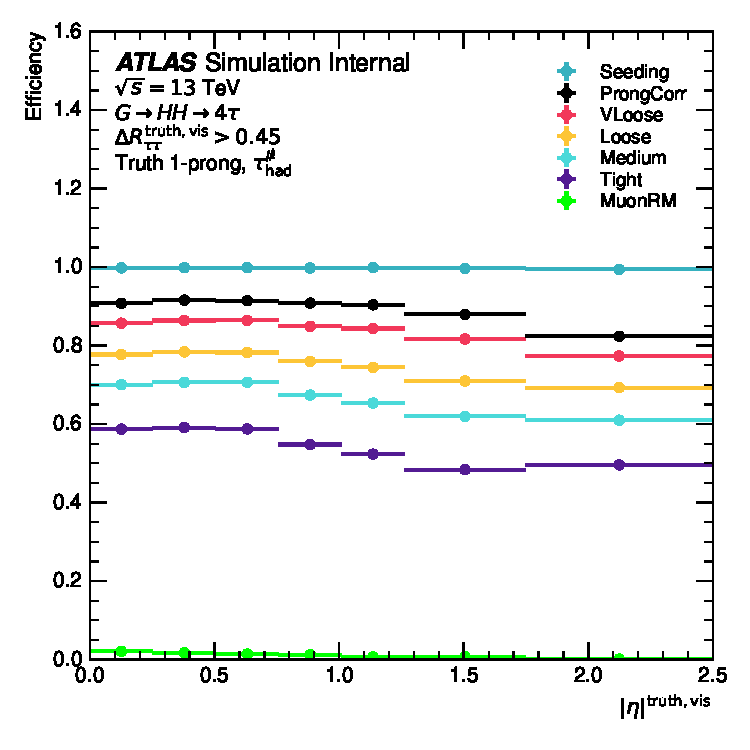
\includegraphics[width=0.50\textwidth]{plots_dev_fin/eff_04dR_eta_new_1p.pdf} \label{fig:murm:eta45dr_1p}}
                % \subfloat[]{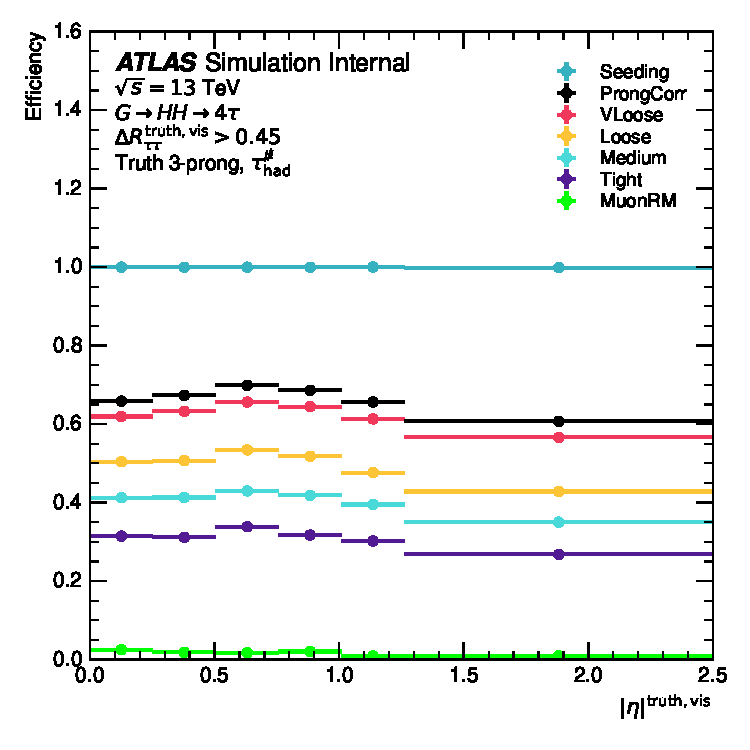
\includegraphics[width=0.50\textwidth]{plots_dev_fin/eff_04dR_eta_new_3p.pdf} \label{fig:murm:eta45dr_3p}}
                % \vspace{-0.45cm} % Adjust the negative space here to bring rows closer
                % \\
                \subfloat[]{\includegraphics[width=0.50\textwidth]{plots_dev_fin/eff_04dR_mu_new_1p.pdf}  \label{fig:murm:mu45dr_1p}}
                \subfloat[]{\includegraphics[width=0.50\textwidth]{plots_dev_fin/eff_04dR_mu_new_3p.pdf}  \label{fig:murm:mu45dr_3p}}
                \caption{The stability of the signal efficiencies of the TauID working points against 
                    the truth transverse momentum~(\protect\subref{fig:murm:pt45dr_1p})~(\protect\subref{fig:murm:pt45dr_3p}), 
                    % absolute pseudorapidity~(\protect\subref{fig:murm:eta45dr_1p})~(\protect\subref{fig:murm:eta45dr_3p}), 
                    and pile-up~(\protect\subref{fig:murm:mu45dr_1p})~(\protect\subref{fig:murm:mu45dr_3p}) for 
                    the truth 1-prong and 3-prong $\tauseed$ jets with $\dRtttruthvis > 0.45$. 
                    In this region, the muon removal should not affect the results. The ``Seeding'' lines indicate the efficiency 
                    of a truth-level $\tauhad$ being reconstructed as $\tauseed$. The ``MuonRM'' lines show the efficiency of 
                    a muon being removed inside the $\tauseed$.}
                \label{fig:murm:45drstability}
            \end{center}
        \end{figure}

        After the removal of the overlapping muon, the precision with which the four-momentum of the $\tauseed$ jet is reconstructed 
        improves significantly. Figure~\ref{fig:murm:sp_resolutions} shows the distributions of 
        the difference between the truth-level and reconstructed variable (residuals) 
        in $\eta$ and $\phi$ before and after muon removal. Compared to the performance before muon removal, the root mean square (RMS)
        widths of the $\eta$ residuals that correspond to the 68\% percentile (core resolution) 
        improves by a factor of 15 for 1-prong $\tauhad$, and by a factor of 20 for 3-prong $\tauhad$. 
        The core resolution in $\phi$ improves also by a factor of 15 times for 1-prong $\tauhad$ and by a factor of 20 for 3-prong $\tauhad$. 
        The distributions of the $\tauhadvis$ transverse energy ($E_\mathrm{T}$) residuals and the relative core (68\%) and 
        tail (95\%) $E_\mathrm{T}$ resolutions as functions of $\tauhadvis$ $E_\mathrm{T}^\mathrm{truth}$ are shown in 
        Figure~\ref{fig:murm:e_resolutions}. These results align nicely with those reported for isolated $\tauhad$ in ref.~\cite{PERF-2014-06}, 
        demonstrating further the effectiveness of the muon-removal technique.

        \begin{figure}[hbtp]
            \begin{center}
                \subfloat[]{\includegraphics[width=0.5\textwidth]{plots_dev_fin/reso_eta_diff_1p.pdf} \label{fig:murm:reso_eta_1p}}
                \subfloat[]{\includegraphics[width=0.5\textwidth]{plots_dev_fin/reso_eta_diff_3p.pdf} \label{fig:murm:reso_eta_3p}}
                \\
                \subfloat[]{\includegraphics[width=0.5\textwidth]{plots_dev_fin/reso_phi_diff_1p.pdf} \label{fig:murm:reso_phi_1p}}
                \subfloat[]{\includegraphics[width=0.5\textwidth]{plots_dev_fin/reso_phi_diff_3p.pdf} \label{fig:murm:reso_phi_3p}}
                \caption{The distributions of the calibrated residuals 
                    $\eta$~(\protect\subref{fig:murm:reso_eta_1p})~(\protect\subref{fig:murm:reso_eta_3p}) and 
                    $\phi$~(\protect\subref{fig:murm:reso_phi_1p})~(\protect\subref{fig:murm:reso_phi_3p}) 
                    before (blue) and after (red) muon removal. The left panel shows the 1-prong case; the right 
                    panel shows the 3-prong case.}
                \label{fig:murm:sp_resolutions}
            \end{center}
        \end{figure}
        \begin{figure}[hbtp]
            \begin{center}
                \subfloat[]{\includegraphics[width=0.5\textwidth]{plots_dev_fin/reso_pt_diff_1p.pdf}\label{fig:murm:reso_pt_1p}}
                \subfloat[]{\includegraphics[width=0.5\textwidth]{plots_dev_fin/reso_pt_diff_3p.pdf}\label{fig:murm:reso_pt_3p}}
                \\
                \subfloat[]{\includegraphics[width=0.5\textwidth]{plots_dev_fin/reso_rela_pt_1p.pdf}\label{fig:murm:reso_rel_pt_1p}}
                \subfloat[]{\includegraphics[width=0.5\textwidth]{plots_dev_fin/reso_rela_pt_3p.pdf}\label{fig:murm:reso_rel_pt_3p}}
                \caption{(\protect\subref{fig:murm:reso_pt_1p})~(\protect\subref{fig:murm:reso_pt_3p}): the distributions of the calibrated transverse energy 
                residuals for $\tauhadvis$ with (red) and without (blue) muon removal. 
                (\protect\subref{fig:murm:reso_rel_pt_1p})~(\protect\subref{fig:murm:reso_rel_pt_3p}): the relative core (68\%) and tail (95\%) 
                $\tauhadvis$ $E_\mathrm{T}$ resolutions as functions of $\tauhadvis$ $E_\mathrm{T}^\mathrm{truth}$. The left 
                plots show the 1-prong case and the right plots show the 3-prong case.}
                \label{fig:murm:e_resolutions}
            \end{center}
        \end{figure}

        Having demonstrated that the reconstruction and identification efficiencies are significantly improved by the $\tauhadmurm$ method, 
        the background rejection power is now illustrated. The production of \ttbar pairs is considered as a source of 
        high $\pt$ heavy-flavour jets, which represents an example background to the $\tauhadmurm$ signal.
        The background rejection ratios at the medium TauID working point, which are defined as the 
        inverted ratios of a mis-reconstructed $\tauseed$ jet being classified as a genuine $\tauhad$ are shown in Figure~\ref{fig:murm:rej},
        as functions of the reconstructed $\tauhad~\pt$, $\tauhad~|\eta|$ and pile-up. For the background rejection plots, and the following 
        receiver operating characteristic (ROC) plots, event-selections are mostly based on the reconstructed properties instead of the truth-level 
        information. A $\tauseed$ jet reconstructed in the background sample is required to have 
        $20\text{ \GeV}<\pt<300\text{ \GeV}$, 
        $|\eta|<2.5$, 
        and to not be truth-matched to a $\tauhad$ lepton from the bottom or top quarks semi-leptonic decay. 
        In addition, a reconstructed muon is required to be found inside the $\tauseed$ jet. 
        The $\tauhad$ candidates in which no muon is present are not considered in Figure~\ref{fig:murm:rej}, as identical 
        TauID results would be expected for these cases.

        \begin{figure}[hbtp]
            \begin{center}
                \subfloat[]{\includegraphics[width=0.5\textwidth]{plots_dev_fin/rej_pt_1p.pdf}  \label{fig:murm:rej_pt_1p}}
                \subfloat[]{\includegraphics[width=0.5\textwidth]{plots_dev_fin/rej_pt_3p.pdf}  \label{fig:murm:rej_pt_3p}}
                \vspace{-0.45cm} % Adjust the negative space here to bring rows closer
                \\
                % \subfloat[]{\includegraphics[width=0.5\textwidth]{plots_dev_fin/rej_eta_1p.pdf} \label{fig:murm:rej_eta_1p}}
                % \subfloat[]{\includegraphics[width=0.5\textwidth]{plots_dev_fin/rej_eta_3p.pdf} \label{fig:murm:rej_eta_3p}}
                % \vspace{-0.45cm} % Adjust the negative space here to bring rows closer
                % \\
                \subfloat[]{\includegraphics[width=0.5\textwidth]{plots_dev_fin/rej_mu_1p.pdf}  \label{fig:murm:rej_mu_1p}}
                \subfloat[]{\includegraphics[width=0.5\textwidth]{plots_dev_fin/rej_mu_3p.pdf}  \label{fig:murm:rej_mu_3p}}
                \caption{The signal rejection ratios for $\tauseed$ jets reconstructed from jets originating from 
                semi-muonic bottom decays in \ttbar events at medium TauID working point, as functions of the 
                reconstructed \pt~(\protect\subref{fig:murm:rej_pt_1p})~(\protect\subref{fig:murm:rej_pt_3p}),
                % $|\eta|$~(\protect\subref{fig:murm:rej_eta_1p})~(\protect\subref{fig:murm:rej_eta_3p}), and 
                and pile-up~(\protect\subref{fig:murm:rej_mu_1p})~(\protect\subref{fig:murm:rej_mu_3p}). 
                The left panel shows the reconstructed 1-prong case, the right panel shows the 3-prong case.}
                \label{fig:murm:rej}
            \end{center}
        \end{figure}

        The background rejection power decreases slightly in the 3-prong case. 
        After the removal of the muon within the $\tau_\mathrm{seed}$ in the case of background events, 
        the TauID algorithm finds it more challenging to reject a semi-leptonic heavy-flavour jet.
        The 1-prong background rejection power increases slightly in 
        the low \pt region after removal of the muon due to two competing phenomena. 
        The muon being removed is often the only charged track found inside the $\tauseed$ jet. 
        Thus, the number of reconstructed 1-prong $\tauseed$ jets decreases significantly. 
        For the remaining reconstructed 1-prong $\tauseed$ jets, 
        the background rejection performance does suffer from the removal of the muon. 

        The signal efficiency observed in the \GHHFourtau samples, and background rejection power observed in the $\ttbar$ sample 
        are combined to form the ROC curves, which are defined as the background rejection factor as a function of the signal efficiency. 
        In addition to the same reconstruction level selections as the background $\tauseed$ jets discussed previously, the 
        signal $\tauseed$ jets are also required to be truth-matched to the $\tmth$ pairs. To minimise the 
        bias introduced by the misalignment of the signal and background momentum spectra, the background events
        are re-weighted so that the \pt distribution of the background samples matches the signal sample. 
        The ROC curves illustrating the performance with and without muon removal are shown in Figure~\ref{fig:murm:roc}. 
        An order-of-magnitude performance gain is seen across the spectrum in both 1-prong and 3-prong curves
        when muon removal is applied.

        \begin{figure}[hbtp]
            \begin{center}
                \subfloat[]{\includegraphics[width=0.5\textwidth]{plots_dev_fin/roc_1p.pdf}\label{fig:murm:roc_1p}}
                \subfloat[]{\includegraphics[width=0.5\textwidth]{plots_dev_fin/roc_3p.pdf}\label{fig:murm:roc_3p}}
                \caption{The receiver operating characteristic (ROC) curves with and without muon removal. 
                (\protect\subref{fig:murm:roc_1p}) shows the reconstructed 1-prong case, 
                (\protect\subref{fig:murm:roc_3p}) shows the 3-prong case.}
                \label{fig:murm:roc}
            \end{center}
        \end{figure}

        To demonstrate the performance of the $\tauhadmurm$ method in reconstructing and 
        identifying di-$\tau$ systems within the \GHHFourtau process, 
        Figure~\ref{fig:murm:effi_mass} presents the combined $\tauhad$ reconstruction and 
        identification efficiencies as a function of the truth-level Graviton mass. 
        The efficiencies shown correspond to the identification of individual di-$\tau$ systems originating from Higgs boson decays.
        Compared to the standard ATLAS TauID, the $\tauhadmurm$ method demonstrates a complete recovery 
        in the identification efficiency for both 1-prong and 3-prong $\tauhad$ decays for high-mass $\GHHFourtau$ samples.
        % This is a potential physics channel that future studies can exploit using the $\tauhadmurm$ method. 
        \begin{figure}[hbtp]
            \begin{center}
                \subfloat[]{\includegraphics[width=0.50\textwidth]{plots_dev_fin/eff_nocut_mG_off_1p.pdf} \label{fig:murm:effi_mass_std_1p}}  
                \subfloat[]{\includegraphics[width=0.50\textwidth]{plots_dev_fin/eff_nocut_mG_off_3p.pdf} \label{fig:murm:effi_mass_std_3p}}  
                \\
                \subfloat[]{\includegraphics[width=0.50\textwidth]{plots_dev_fin/eff_nocut_mG_new_1p.pdf}\label{fig:murm:effi_mass_new_1p}}
                \subfloat[]{\includegraphics[width=0.50\textwidth]{plots_dev_fin/eff_nocut_mG_new_3p.pdf}\label{fig:murm:effi_mass_new_3p}}
                \caption{The signal efficiencies of the TauID working points, as a function of the truth-level Graviton mass, $m_G^\mathrm{truth}$, 
                    for truth 1-prong~(\protect\subref{fig:murm:effi_mass_std_1p}) and 3-prong~(\protect\subref{fig:murm:effi_mass_std_3p}) $\tauhad$ with the standard ATLAS TauID;
                    and for truth 1-prong~(\protect\subref{fig:murm:effi_mass_new_1p}) and 3-prong~(\protect\subref{fig:murm:effi_mass_new_3p}) $\tauhad$ with the $\tauhadmurm$ method.
                    The efficiencies shown correspond to the identification of individual di-$\tau$ systems originating from Higgs boson decays.
                    The ``Seeding'' lines indicate the efficiency 
                    of a truth-level $\tauhad$ being reconstructed as $\tauseed$. 
                    the ``ProngCorr'' line shows the efficiency of a truth-level $\tauhad$ being 
                    reconstructed with the correct number of associated charged-particle tracks.
                    The ``MuonRM'' lines show the efficiency of 
                    a muon being removed inside the $\tauseed$.
                }
                \label{fig:murm:effi_mass}
            \end{center}
        \end{figure}

\FloatBarrier

\section{Validation of the $\tauhadmurm$ method in the $\Zttmuhad$ channel} \label{sec:Zttbench}
    \subsection{The collinear assumptions and event reconstruction} \label{sec:collinear_assumptions_and_evt_reco}
        The $\tauhadmurm$ method was developed for searches like high-mass BSM physics, such as the \GHH process, 
        as described in Section~\ref{sec:murm}. However, it is useful to test its performance considering a SM process.
        The Drell-Yan production of a $Z$ boson in association with high-$p_T$ jets from QCD initial-state 
        radiation is considered as benchmark process.

        The detector signature of the boosted $\Zttmuhad$ process includes one hadronically decaying $\tau$ and a muon, 
        in association with significant missing transverse momentum ($\MET$) from the neutrinos produced in the two 
        $\tau$ decays. In this case, the hadronically decaying 
        $\tau$ and the muon are likely to fall within the same $\tauseed$ jet. In well measured events, the vector sum 
        of the transverse momenta of the three neutrinos dominates the measured $\MET$, which in azimuth direction should lie 
        between the observed muon and the $\tauhad$. Also, on average, the $\MET$ should be closer in azimuth to the muon, 
        because the leptonic decay produces two neutrinos and the hadronic decay only one.

        Without incorporating $\MET$, reconstructing the Z invariant mass is not possible. However, it is possible to approximate 
        the momenta of the neutrinos with the collinear assumptions~\cite{ELLIS1988221} as follows:
        \begin{itemize}
            \item the transverse momenta of the three neutrinos dominate the measured $\MET$, and other contributions are negligible;
            \item each $\tau$ lepton is sufficiently boosted such that the neutrino (or pair of neutrinos) produced in its decay is collinear with its visible decay products
            \footnote{In events in which the $\MET$ lies outside the azimuthal angle 
                between the visible decay products of the tau leptons (e.g., due to detector resolution), the 
                $\MET$ is projected onto the direction of the nearest visible decay, and the neutrino momentum 
                associated with the other tau lepton is set to zero. Furthermore, events for which collinear 
                reconstruction is not possible, i.e., with $\MET$ deviating by more than $90^{\circ}$ from the muon 
                or the $\tauhadmurm$ in $\deltaphi$, are discarded.}.
        \end{itemize}
        Together with the momenta of the visible decay products, this procedure allows the momenta of 
        the two tau leptons, and hence the momentum, transverse momentum ($\ptcol$), and mass ($\mcol$) 
        of the system produced by the decay of the $Z$ boson, to be reconstructed.
        The jets recoiling against the Z boson are reconstructed using the anti-$k_t$ algorithm with a radius 
        parameter of 0.4, which operates on topological clusters calibrated to the EM scale~\cite{JETM-2018-05}.
    \subsection{Event-selection} \label{sec:ZttSelection}
        Candidate events are required to be triggered by an un-prescaled single-muon trigger or an un-prescaled $\MET$ trigger.
        The thresholds of the $\pt$ required to fire each trigger vary for different data-taking periods. For the single muon trigger,
        the $\pt$ requirement for triggers with object isolation requirement ranges from 20-26~$\GeV$, while the $\pt$ threshold for non-isolated muons remains constant at 50~$\GeV$. 
        The \MET triggers have a $\pt$ threshold of 70~$\GeV$ for the 2015 data-taking period and remain constant at 110~$\GeV$ for the rest of Run~2. 
        Approximately 97\% of  $\Zttmuhad$ MC events that pass the final signal selection criteria pass the trigger selection.
        For the signal-region (SR) selection, events passing the trigger requirements are required 
        to have at least one muon-removal $\tauhad$ object with $\pt > 15~\GeV$ and a RNN TauID score > 0.1, 
        excluding pseudorapidity ranges $1.37 < |\eta| < 1.52$ and $|\eta| > 2.5$. This selection 
        implies that at least one reconstructed muon passing ``Medium'' ID is inside the cone of the selected 
        $\tauhadmurm$. An additional $\pt > 10~\GeV$ requirement on the corresponding muon is imposed. 
        In this study, the overlap removal (OLR) between muons and $\tauhad$ candidates is turned off. 
        The default overlap removal algorithm as described in Ref.~\cite{HIGG-2019-09} would remove 
        the $\tauhadmurm$ candidates if the muon removal method is successful. 
        To suppress background from events containing heavy flavour jets, events are vetoed if they 
        contain any jet that satisfies the DL1d based $b$-tagging algorithm at an 85\% efficiency working point~\cite{FTAG-2019-07}.
        The invariant mass, $\mvis$, of the visible $\tmth$ system is required to satisfy $\mvis > 5$~GeV. 
        The signed $\deltaphi$ between the muon and $\MET$ ($\deltamumet$) is required to be $-0.1 < \deltamumet < 0.4$ . 
        The sign of $\deltamumet$ is determined by the direction of the $\tauhad$. 
        If the $\MET$ is inside the opening angle of the muon and the $\tauhad$ or if the $\MET$ is outside 
        the opening angle but closer to the muon, then the sign is positive; otherwise, it is negative. 
        Since the focus of the analysis is the boosted $\Zttmuhad$ process, a loose requirement $\mcol > 40$~GeV, 
        and a requirement $\ptcol > 250$~GeV are applied. 
        To study the QCD multijets background contributions not described by the MC, 
        a control-region (CR) is defined with the same selection requirements as the SR, except that the
        muon and $\tauhadmurm$ have the same charge, and there is no requirement on $\deltamumet$ or 
        number of jets passing the $b$-tagging requirement.
        Table~\ref{tab:murm:evt_sel} summaries the event-selection requirements for SR and CR.
        \begin{table}[htbp]
            \caption{Summary of event-selection requirements}
            \label{tab:murm:evt_sel}
            \centering
            \scriptsize
            \begin{tabular}{lcc}
                \toprule
                Object & Signal-Region Selection & Control-Region Selection \\
                \midrule
                $\tauhadmurm$  & \begin{tabular}{c} $0 < |\eta| < 1.37$ or $1.52 < |\eta| < 2.5$ \\ Jet RNN score > 0.1 \\ $\pt > 15$~GeV \\ 1 or 3 charged tracks \end{tabular}   & \begin{tabular}{c} $0 < |\eta| < 1.37$ or $1.52 < |\eta| < 2.5$ \\ Jet RNN score > 0.1 \\ $\pt > 15$~GeV \\ 1 or 3 charged tracks \end{tabular} \\
                \midrule
                $\mu$          & \begin{tabular}{c} $\pt > 10~\GeV$ \\ ``Medium'' ID \end{tabular}                                      & \begin{tabular}{c} $\pt > 10~\GeV$ \\ ``Medium'' ID \end{tabular} \\       
                \midrule
                $\tmth$ system & \begin{tabular}{c} $\mvis > 5~\GeV$ \\ $-0.1 < \deltamumet < 0.4$ \\ $\mcol > 40~\GeV$ \\ $\ptcol > 250~\GeV$ \\ no $b$-tag jet at 85\% efficiency working point \\ Opposite Sign muon and $\tauhadmurm$ \end{tabular} &     \begin{tabular}{c} $\mvis > 5~\GeV$ \\ $\mcol > 40~\GeV$ \\ $\ptcol > 250~\GeV$ \\ Same Sign muon and $\tauhadmurm$\end{tabular} \\
                \bottomrule
            \end{tabular}
        \end{table}

        Figures~\ref{fig:murm:RNN_score}$-$\ref{fig:murm:pt_mu} illustrate the distributions of selected variables in the SR and CR. 
        As shown in Figure~\ref{fig:murm:m_col}, the data and MC predictions 
        agree well for $\mcol > 40$~GeV in both the SR and CR, indicating that QCD processes not modelled 
        by the MC simulations contribute negligibly to the background in the selected signal sample. The collinear 
        mass reconstruction effectively reconstructs the di-tau system mass, as seen in the peak corresponding to the $Z$ boson mass 
        in Figure~\ref{fig:murm:m_col}(a). The shape of the \mcol distribution for signal 
        Drell-Yan events is very different from that seen
        in inclusive production, with a much larger fraction of the signal events in the 
        region $40 < \mcol < 70$ GeV relative to that at the Z boson peak.  
        This is a result of the sharply falling distribution in Z boson \pT for Drell-Yan 
        production, coupled with the fact that the opening angle of boosted \tmth systems 
        decreases with decreasing \mcol.
        Due to the the $\mcol > 40$~GeV requirement, the number of events with $\ptcol$ below 250~GeV is very low. 
        This highlights the fact that the $\tauhadmurm$ reconstruction picks up $\tauhad$ only with a sufficiently high boost. 
        An excess of data compared to the MC prediction is observed in the $\pt < 35 \GeV$ region within the SR. 
        Further investigation has identified this discrepancy as a result of mis-modelling of the $\tauhad$ kinematics in 
        the $\Ztautau$ MC simulation~\cite{Dong:2899443}.
        % No significant excess of signal events around the Higgs boson mass is observed. This is consistent with expectations, 
        % given the lower production cross-section of the Higgs boson compared to the $Z$ boson.
        \begin{figure}[htbp]
            \centering
            \subfloat[]{
                \includegraphics[width=0.50\textwidth]{plots_ztt_rebin_scaled_syst/leading_tau_rnn_SR.pdf}
                \label{fig:murm:SR_RNN_score}
            }
            \subfloat[]{
                \includegraphics[width=0.50\textwidth]{plots_ztt_rebin_scaled_syst/leading_tau_rnn_CR_new_final.pdf}
                \label{fig:murm:CR_RNN_score}
            }
            \caption{
                The distribution of the RNN jet score for $\tauhadmurm$: (\protect\subref{fig:murm:SR_RNN_score}) in the SR and,
                (\protect\subref{fig:murm:CR_RNN_score}) in the CR. 
                ``Top'' represents the predicted contributions from the SM $\ttbar$, single-top, and $tW$ processes. 
                ``DiBoson'' indicates the contributions from $WW$, $WZ$, and $ZZ$ processes. 
                ``Other'' includes the contributions from the $Z\rightarrow ll$+jets and $W$+jets background processes. 
                ``$\Ztautau$+jets'' represents the contributions from the signal process.
                The uncertainties shown include both statistical and systematic uncertainties.
            }
            \label{fig:murm:RNN_score}
        \end{figure}

        \begin{figure}[htbp]
            \centering
            \subfloat[]{
                \includegraphics[width=0.50\textwidth]{plots_ztt_rebin_scaled_syst/omega_noscale_SR.pdf}
                \label{fig:murm:SR_s_dphi}
            }
            \subfloat[]{
                \includegraphics[width=0.50\textwidth]{plots_ztt_rebin_scaled_syst/omega_noscale_CR_new_final.pdf}
                \label{fig:murm:CR_s_dphi}
            }
            \caption{
                The distribution of $\deltamumet$ with all other event-selection criteria 
                applied in the SR is shown in (\protect\subref{fig:murm:SR_s_dphi}); 
                the straight lines indicate the positions of the selection requirements.
                The same distribution in the CR is shown in (\protect\subref{fig:murm:CR_s_dphi}). 
                ``Top'' represents the predicted contributions from the SM $\ttbar$, single-top, and $tW$ processes. 
                ``DiBoson'' indicates the contributions from $WW$, $WZ$, and $ZZ$ processes. 
                ``Other'' includes the contributions from the $Z\rightarrow ll$+jets and $W$+jets background processes. 
                ``$\Ztautau$+jets'' represents the contributions from the signal process.
                The uncertainties shown include both statistical and systematic uncertainties.
            }
            \label{fig:murm:s_dphi}
        \end{figure}

        \begin{figure}[htbp]
            \centering
            \subfloat[]{
                \includegraphics[width=0.50\textwidth]{plots_ztt_rebin_scaled_syst/m_tt_colin_SR.pdf}
                \label{fig:murm:SR_m_col}
            }
            \subfloat[]{
                \includegraphics[width=0.50\textwidth]{plots_ztt_rebin_scaled_syst/m_tt_colin_CR_new_final.pdf}
                \label{fig:murm:CR_m_col}
            }
            \caption{
                The distribution of the $\mcol$: (\protect\subref{fig:murm:SR_m_col}) in the SR, and,
                (\protect\subref{fig:murm:CR_m_col}) in the CR. 
                ``Top'' represents the predicted contributions from the SM $\ttbar$, single-top, and $tW$ processes. 
                ``DiBoson'' indicates the contributions from $WW$, $WZ$, and $ZZ$ processes. 
                ``Other'' includes the contributions from the $Z\rightarrow ll$+jets and $W$+jets background processes. 
                ``$\Ztautau$+jets'' represents the contributions from the signal process.
                The uncertainties shown include both statistical and systematic uncertainties.
            }
            \label{fig:murm:m_col}
        \end{figure}

        \begin{figure}[htbp]
            \centering
            \subfloat[]{
                \includegraphics[width=0.50\textwidth]{plots_ztt_rebin_scaled_syst/pt_tt_colin_SR.pdf}
                \label{fig:murm:SR_pt_col}
            }
            \subfloat[]{
                \includegraphics[width=0.50\textwidth]{plots_ztt_rebin_scaled_syst/pt_tt_colin_CR_new_final.pdf}
                \label{fig:murm:CR_pt_col}
            }
            \caption{
                The distribution of the $\ptcol$: (\protect\subref{fig:murm:SR_pt_col}) in the SR, and,
                (\protect\subref{fig:murm:CR_pt_col}) in the CR. 
                ``Top'' represents the predicted contributions from the SM $\ttbar$, single-top, and $tW$ processes. 
                ``DiBoson'' indicates the contributions from $WW$, $WZ$, and $ZZ$ processes. 
                ``Other'' includes the contributions from the $Z\rightarrow ll$+jets and $W$+jets background processes. 
                ``$\Ztautau$+jets'' represents the contributions from the signal process.
                The uncertainties shown include both statistical and systematic uncertainties.
            }
            \label{fig:murm:pt_col}
        \end{figure}

        \begin{figure}[htbp]
            \centering
            \subfloat[]{
                \includegraphics[width=0.50\textwidth]{plots_ztt_rebin_scaled_syst/leading_tau_pt_SR.pdf}
                \label{fig:murm:SR_pt_tau}
            }
            \subfloat[]{
                \includegraphics[width=0.50\textwidth]{plots_ztt_rebin_scaled_syst/leading_tau_pt_CR_new_final.pdf}
                \label{fig:murm:CR_pt_tau}
            }
            \caption{
                The distribution of the \pt of the $\tauhadmurm$: (\protect\subref{fig:murm:SR_pt_tau}) in the SR  and,
                (\protect\subref{fig:murm:CR_pt_tau}) in the CR. 
                ``Top'' represents the predicted contributions from the SM $\ttbar$, single-top, and $tW$ processes. 
                ``DiBoson'' indicates the contributions from $WW$, $WZ$, and $ZZ$ processes. 
                ``Other'' includes the contributions from the $Z\rightarrow ll$+jets and $W$+jets background processes. 
                ``$\Ztautau$+jets'' represents the contributions from the signal process.
                The uncertainties shown include both statistical and systematic uncertainties.
            }
            \label{fig:murm:pt_tau}
        \end{figure}

        \begin{figure}[htbp]
            \centering
            \subfloat[]{
                \includegraphics[width=0.50\textwidth]{plots_ztt_rebin_scaled_syst/muon_pt_SR.pdf}
                \label{fig:murm:SR_pt_mu}
            }
            \subfloat[]{
                \includegraphics[width=0.50\textwidth]{plots_ztt_rebin_scaled_syst/muon_pt_CR_new_final.pdf}
                \label{fig:murm:CR_pt_mu}
            }
            \caption{
                The distribution of the \pt of the muon removed from the $\tauhadmurm$: 
                (\protect\subref{fig:murm:SR_pt_mu}) in the SR and,
                (\protect\subref{fig:murm:CR_pt_mu}) in the CR. 
                ``Top'' represents the predicted contributions from the SM $\ttbar$, single-top, and $tW$ processes. 
                ``DiBoson'' indicates the contributions from $WW$, $WZ$, and $ZZ$ processes. 
                ``Other'' includes the contributions from the $Z\rightarrow ll$+jets and $W$+jets background processes. 
                ``$\Ztautau$+jets'' represents the contributions from the signal process.
                The uncertainties shown include both statistical and systematic uncertainties.
            }
            \label{fig:murm:pt_mu}
        \end{figure}

    \subsection{Systematic uncertainties} \label{sec:sys_uncertainties}
        The dominant source of systematic uncertainty in the comparison between the observed and expected yields in the SR is the modelling of the cross-section 
        for $Z$ boson production. As discussed in Section~\ref{sec:DataAndMCs}, a +10\% 
        correction is applied to the predicted numbers for $\Ztautau$ events, 
        with the full size of this correction quoted as a systematic uncertainty.

        The most significant sources of experimental systematic uncertainties are TauID and tau energy scale~(4\%), 
        jet energy scale and resolution~(2\%), \MET~(2\%)~\cite{Baron:2887993}, and luminosity~(0.8\%)~\cite{DAPR-2021-01}.
\section{Results} \label{sec:results}
    % In this section, the results of the $\Ztautau$ benchmark analysis are presented, 
    % focusing on the signal and background distributions, event yields in the signal and control 
    % regions, and some important observations. 
    In order to understand the performance improvement 
    comparing to the standard ATLAS $\tauhad$ reconstruction and identification,
    Figure~\ref{fig:murm:SRcmp} shows comparisons between the data and MC predictions for \mcol\ distributions corresponding to various signal selections;
    Figure~\ref{fig:murm:SR_m} shows the SR defined in Section~\ref{sec:ZttSelection};
    Figure~\ref{fig:murm:SR_std_m} shows the sample \SRstd, which uses the standard ATLAS $\tauhad$ candidates;
    without the muon removal, but otherwise corresponds to the same event-selection as SR;
    Figure~\ref{fig:murm:SR_tight_m} shows the sample \SRtight, which
    imposes an additional ``tight'' RNN TauID requirement on the $\tauhadmurm$ candidates, but otherwise corresponds
    to the SR selection;
    Figure~\ref{fig:murm:SR_tight_std_m} shows the sample \SRtightstd, which
    imposes an additional ``tight'' RNN TauID requirement and uses the standard $\tauhad$, without muon removal.
    
    \begin{figure}[htbp]
        \centering
        \subfloat[]{
            \includegraphics[width=0.50\textwidth]{plots_ztt_rebin_scaled_syst/m_tt_colin_SR_cmp.pdf}
            \label{fig:murm:SR_m}
        }
        \subfloat[]{
            \includegraphics[width=0.50\textwidth]{plots_ztt_rebin_scaled_syst/m_tt_colin_SR_std_cmp.pdf}
            \label{fig:murm:SR_std_m}
        }
        \\
        \subfloat[]{
            \includegraphics[width=0.50\textwidth]{plots_ztt_rebin_scaled_syst/m_tt_colin_SR_tight_cmp.pdf}
            \label{fig:murm:SR_tight_m}
        }
        \subfloat[]{
            \includegraphics[width=0.50\textwidth]{plots_ztt_rebin_scaled_syst/m_tt_colin_SR_tight_std_cmp.pdf}
            \label{fig:murm:SR_tight_std_m}
        }
        \caption{The distributions of $\mcol$ corresponding to the various signal selections defined in the text: 
            (\protect\subref{fig:murm:SR_m}) SR, 
            (\protect\subref{fig:murm:SR_std_m}) \SRstd, 
            (\protect\subref{fig:murm:SR_tight_m}) \SRtight, and
            (\protect\subref{fig:murm:SR_tight_std_m})  \SRtightstd.
            SR, $\SRtight$ and CR are with the $\tauhadmurm$ method, while $\SRstd$ and $\SRtightstd$ are with the standard ATLAS TauID.
        }
        \label{fig:murm:SRcmp}
    \end{figure}
    Table~\ref{tab:murm:n_evt} shows the event yields corresponding to the various signal selections defined previously,
    and the CR. The number of events observed in 
    the ATLAS Run 2 data are given, as well as the SM-predicted contributions from signal and background processes. 
        
    Compared with the  the standard ATLAS TauID, the $\tauhadmurm$ achieves around 
    three times more signal events in the SR, while maintaining a similar number of background events. 
    In the \SRtight\ region, the number of signal events 
    is four times higher than using the nominal $\tauhadstd$, again while maintaining a similar number of background events.
    \begin{table}[htbp]
        \caption{
            Event yields in different event-selections, as defined in the text. 
            SR, $\SRtight$ and CR are with the $\tauhadmurm$ method, while $\SRstd$ and $\SRtightstd$ are with the standard ATLAS TauID.
            The uncertainties quoted are statistical only. The $Z\rightarrow\tau\tau$ contribution
            is scaled by +10\% to account for the difference between the MC prediction and the data.
        }
        \label{tab:murm:n_evt}
        \centering
        \scriptsize
        \begin{tabular}{l|cc|cc|c}
            \toprule
                                    & SR                & $\SRstd$                  & $\SRtight$                & $\SRtightstd$                         & CR   \\
            \midrule
            Data                    & $1155 \pm 34$     & $616 \pm 25$              & $705 \pm 27$              & $210 \pm 14$                          & $286 \pm 17$     \\ 
            MC total                & $1188 \pm 10$     & $574 \pm 8$               & $733 \pm 7$               & $223 \pm 4$                           & $302 \pm 7$ \\
            \midrule
            $\Ztautau$              & $958\pm 8$        & $339 \pm 4$               & $646 \pm 6$               & $124 \pm 2$                           & $20 \pm 1$ \\
            Di-boson                & $93 \pm 1$        & $37 \pm 1$                & $51 \pm 1$                & $15 \pm 0$                            & $39 \pm 1$ \\
            Top                     & $70 \pm 3$        & $153 \pm 5$               & $26 \pm 2$                & $67 \pm 3$                            & $165 \pm 5$  \\
            Other                   & $66 \pm 4$        & $45 \pm 4$                & $10\pm 2$                 & $17 \pm 2$                            & $78 \pm 4$ \\
            \bottomrule
        \end{tabular}
    \end{table}
    Subtracting the expected background yield in the SR of $230\pm 5$ events gives a 
    measured yield for $\Zttmuhad$ of $925 \pm 34$ events. 
    This can be compared to the expected yield for \Zttmuhad\ of $958 \pm 8~\text{(stat.)}\pm~115~\text{(syst.)}$ events. 
    Adding all sources of statistical and systematic uncertainty results in a total uncertainty of 12\%. 
    The ratio between the background-subtracted data and the expected signal yields is $0.97 \pm 0.12$. 


\FloatBarrier

\section{Summary and conclusion} \label{sec:conclusion}
    In this chapter, the case of a highly boosted pair of $\tau$ leptons is considered, 
    in which one $\tau$ decays produce a muon and the other $\tau$ decays hadronically, 
    with the visible decay products reconstructed within a single $\tauseed$ jet. In such 
    cases, the standard ATLAS TauID for hadronically decaying $\tau$ leptons fails due 
    to the presence of the nearby muon.

    The development of a muon-removal procedure using samples of high-mass $\GHHFourtau$ 
    events is described. This $\tauhadmurm$ method recovers the \tauhad\ reconstruction and identification 
    efficiencies to the level expected for isolated \tauhad\ decays for all TauID working 
    points. The measurement precision for the kinematic properties of the visible \tauhad\ 
    system is similarly recovered. The $\tauhadmurm$ objects are benchmarked by selecting 
    a sample of highly boosted $\Zttmuhad$ final states using the complete Run 2 dataset 
    recorded by the ATLAS detector. Good agreement is found between data and MC predictions 
    in both the signal $\Zttmuhad$ region and in a control-region in which the muon and 
    \tauhad\ candidate have same-sign charges. The comparison of rates in the signal 
    region gives a ratio between the background-subtracted data and the expected 
    signal yields of $0.97 \pm 0.12$. 

    The results presented in this chapter demonstrate the effectiveness of the $\tauhadmurm$ 
    objects in enhancing the signal sensitivity of the boosted $\tmth$ channel. The 
    observed good agreement between the data and the SM theory predictions in the signal 
    region reaffirms the robustness of the newly developed object. 

    %!TEX root = ../thesis.tex
%*******************************************************************************
%****************************** Third Chapter **********************************
%*******************************************************************************
\chapter{The electron-removal method for boosted \teth reconstruction}

\graphicspath{{1_MainChapters/Chap6_ElecRM/figs/}}

\section{Introduction}
    \label{sec:erm:intro}
    Similar to the \tmth channel, if an electron lies within the \tauseed jet,
    the standard TauReco and TauID algorithm is not able to reconstruct and identify the \tauhad. 
    Figure \ref{fig:erm:dR_eff_off} shows the combined reconstruction and 
    identification efficiency as a function of the truth-level $\dRvistt$. 
    The efficiency of the TauReco and TauID algorithms drop significantly when the $\dRvistt$ is less than 0.4, as the electron begin to merge with the \tauseed jet. As a result, the 
    possibility of reconstructing the correct number of \tauhad tracks is significantly reduced, 
    and the \tauhad identification efficiency drops significantly in all the WPs.
    \begin{figure}[htbp]
        \centering
        \includegraphics[width=0.495\textwidth]{plots_dev/eff_nocut_dR_off_1p.pdf}
        \includegraphics[width=0.495\textwidth]{plots_dev/eff_nocut_dR_off_3p.pdf}
        \caption{The combined reconstruction and identification efficiency of the 
        standard TauReco and TauID as a function of the truth-level $\dRvistt$. The
        efficiency is shown for the different working points of the TauID algorithm. 
        In addition, the ``Reco'' and ``ProngCorr'' efficiencies are shown, 
        which are the efficiency of the \tauhad being seeded, and the efficiency 
        of the TauRec algorithm to reconstruct the correct number of tracks in the 
        \tauhad, respectively.}
        \label{fig:erm:dR_eff_off}
    \end{figure}
    Having demonstrated the success of the \tauhadmurm, we proposed a 
    similar method for the \teth channel, the electron-removal \tauhad (\tauhaderm).

    The \tauhaderm reconstruction is however much more challenging 
    than the \tauhadmurm, technically and physically.
    The electron is not a minimum ionising particle (MIP) like the muon.
    Its energy deposition in the calorimeter makes it much more complicated to remove.
    The electron showers in the calorimeter, depositing most of its energy 
    in the EM calorimeter. In very highly boosted cases, 
    the electron can also deposit significant energy in the hadronic calorimeter. 
    In the context of the \tauhaderm, the electron cluster can merge with 
    the \tauhad clusters, making the separation of the clusters difficult.
    The presence of the electron in the \tauseed jet can also drag the barycentre 
    of the \tauhad to the direction of the electron. 
    Simply removing the electron from the \tauseed jet results in a \tauhad with 
    a shifted axis. with some of the \tauhad decay products being outside 
    the core-cone of the \tauseed jet. This problem severely affects the efficacy of a
    simple electron-removal method. 

    In Section~\ref{sec:erm:method}, we present an accretive method to reconstruct the 
    \tauhaderm in the presence of an electron. We also show that the accretive 
    \tauhaderm can be reconstructed with high 
    efficiency in the region where the $\dRvistt > 0.2$. 
    The energy and spatial resolution of the \tauhaderm are presented in
    Section~\ref{sec:erm:ereso}.
    An initial benchmark of the \tauhaderm in the \Zttehad channel is presented 
    in Section~\ref{sec:erm:benchmark}.
    The summary and outlook of the \tauhaderm reconstruction is presented 
    in Section~\ref{sec:erm:summary}.

\section{Accretive $\tauhaderm$ reconstruction method}
    \label{sec:erm:method}
    For the development of \tauhaderm, the \GHHFourtau MC samples as described in Chapter 5 are used. 
    However, instead of utilising the full mass range of the \GHHFourtau 
    samples, only the $m_G=1500$ \GeV sample is considered due to limitations in resources for 
    custom ATLAS MC production.
    This sample is chosen because it covers the $\Delta R^\mathrm{truth}_\mathrm{\tau\tau}$ 
    range from 0.1 to 0.6, which represents the most comprehensive region for \tauhaderm reconstruction.
    The accretive \tauhaderm reconstruction is a six-step process for every event:
    \begin{enumerate}
        \item The first step is to identify the electrons that satisfy the MediumLH WP, without isolation requirements.
        \item The second step is to remove the tracks and calorimeter clusters associated with the electrons from the event.
        \item Thirdly, using the remaining LCTopo clusters and tracks, the \tauseed jets are re-clustered with the \antikt algorithm with $R=0.4$.
        \item In the fourth step, re-clustered electron-free \tauseed jets with $\dRttReco > 0.6$ to any identified electron are removed from the event, as they should not be affected by the electron.
        \item Then, the electron-free track and cluster collections are supplied to the TauRec algorithm, which reconstructs the \tauhaderm candidates from the remaining \tauseed jets.
        \item Finally, the \tauhaderm candidates are identified using the standard TauID algorithm.
    \end{enumerate}

    Figure \ref{fig:erm:eff_dR_erm} shows the TauID efficiency of the accretive \tauhaderm reconstruction method as a function of the truth-level $\dRvistt$.
    \begin{figure}[htbp]
        \centering
        \includegraphics[width=0.495\textwidth]{plots_dev/eff_nocut_dR_new_1p.pdf}
        \includegraphics[width=0.495\textwidth]{plots_dev/eff_nocut_dR_new_3p.pdf}
        \caption{The combined reconstruction and identification efficiency of the accretive \tauhaderm reconstruction method as a function of the truth $\dRvistt$. The
        efficiency is shown for every working points of the TauID algorithm. In addition, the ``Reco'', ``ElecRM'', and ``ProngCorr'' efficiencies are shown, which is the efficiency of the
        \tauhad being seeded, the efficiency of the electron-removal, and the efficiency of the TauRec algorithm reconstructing the correct number of tracks, respectively.}
        \label{fig:erm:eff_dR_erm}
    \end{figure}
    Compared to more than 90\% MediumLH efficiency for isolated electrons at high \pT~\cite{EGAM-2021-01}, 
    the ``ElecRM'' efficiency is significantly lower, at around 70\% in $\dRvistt > 0.2$ region. 
    Below this threshold, the electron ID efficiency drops significantly, as the electron and \tauhad clusters start to merge. 
    The TauID efficiency of the \tauhaderm is significantly 
    higher than the standard TauID algorithm in this region,
    but not as high as the TauID efficiency for isolated \tauhad candidates.

    If we only consider the case where the overlapping electron is identified and removed, the performance as functions of truth-level 
    $\dRvistt$, $\pT{}_{\tau}^\mathrm{truth,vis}$, and $|\eta|^\mathrm{truth, vis}$ are shown in 
    Figure \ref{fig:erm:eff_new_trkrm}.
    In such cases, the TauID efficiency in various WPs in the $\dRvistt > 0.2$ 
    region are completely recovered.
    The ``ProngCorr'' efficiency is also recovered to more than 90\% in the $\dRvistt > 0.2$ 
    region for 1-prong \tauhaderm.
    The ``ProngCorr'' efficiency reaches 80\% for 3-prong \tauhaderm at low-\pT. 
    In 3-prong case, higher track multiplicity makes it more challenging to reconstruct \tauhad, especially in high \pT region.
    When the electron is identified and removed, the TauID efficiency
    behaves similarly to the standard TauID algorithm and the muon-removal method. 
    The similarity shows that the accretive \tauhaderm 
    objects can be treated as isolated \tauhad objects.
    In all cases, the electron-removal, TauRec, and TauID efficiencies drops significantly in 
    the $\dRvistt < 0.2$ region. As the electron and \tauhad clusters start to merge in this region, 
    both the identification of the electron and the reconstruction of the \tauhad becomes more challenging.

    \begin{figure}[htbp]
        \centering
        \subfloat[]{
            \includegraphics[width=0.5\textwidth]{plots_dev/eff_02dR04_erm_pt_new_1p.pdf}
            \includegraphics[width=0.5\textwidth]{plots_dev/eff_02dR04_erm_pt_new_3p.pdf}
            \label{fig:eff_pt_new_trkrm_unique}
        }
        \\
        \subfloat[]{
            \includegraphics[width=0.5\textwidth]{plots_dev/eff_02dR04_erm_eta_new_1p.pdf}
            \includegraphics[width=0.5\textwidth]{plots_dev/eff_02dR04_erm_eta_new_3p.pdf}
            \label{fig:eff_abseta_new_trkrm}
        }
        \caption{The efficiency of the accretive \tauhaderm reconstruction method as a function of the truth-level
        $\pT{}_{\tau}^\mathrm{truth,vis}$ (\protect\subref{fig:eff_pt_new_trkrm_unique}), 
        and $|\eta|^\mathrm{truth, vis}$ (\protect\subref{fig:eff_abseta_new_trkrm}), 
        where the electron is identified and removed. The
        efficiency is shown for the different working points of the TauID algorithm for 1-prong and 3-prong. In addition, the ``ElecRM'', and ``ProngCorr'' efficiencies are 
        the efficiency of the electron-removal, and 
        the efficiency of the TauRec algorithm to reconstruct the correct number of tracks in the \tauhad, respectively.}
        \label{fig:erm:eff_new_trkrm}
    \end{figure}

    This method is much more challenging technically compared to the case for \tauhadmurm, 
    due to the limitations of the event-level thinning in the ATLAS xAOD Event Data Model (EDM). 
    TauRec algorithms rely on the individual calorimeter cell information to function.
    After the ATLAS Tier-0 reconstruction, the calorimeter cell information is discarded 
    unless they are associated with a reconstructed standard \tauhad candidates.
    The \tauhaderm objects contains different clusters than the standard \tauhad objects, 
    in which the cells are not preserved in the xAOD.
    As a result, the \tauhaderm reconstruction is not possible in the standard ATLAS xAOD EDM. 
    It can only be performed in the ATLAS Tier-0 reconstruction. 
    The \tauhaderm objects originate from a different set of $\tauseed$ jets,
    meaning that unlike the $\tauhadmurm$, there is no direct equivalent in the standard \tauhad collection. 
    To save Tier-0 CPU usage and xAOD storage, only the \tauhaderm objects that are within 
    $\dRvistt < 0.6$ are saved in the xAOD.

\section{Energy and spatial resolution of the \tauhaderm}
    \label{sec:erm:ereso}
    \begin{figure}[!tb]
        \centering
        \subfloat[]{
            \includegraphics[width=0.5\textwidth]{plots_dev/reso_pt_diff_1p.pdf}
            \includegraphics[width=0.5\textwidth]{plots_dev/reso_pt_diff_3p.pdf}
            \label{fig:diff_pt}
        }
        \\
        \subfloat[]{
            \includegraphics[width=0.5\textwidth]{plots_dev/reso_rela_pt_1p.pdf}
            \includegraphics[width=0.5\textwidth]{plots_dev/reso_rela_pt_3p.pdf}
            \label{fig:ereso_abseta_new_trkrm}
        }
        \caption{The distributions of the calibrated transverse energy residuals for $\tauhadvis$ with
                \tauhaderm (red) and \tauhad (blue) are shown in (\protect\subref{fig:diff_pt}). 
                The relative core (68\%) and tail (95\%) $\tauhadvis$ $p_\mathrm{T}$ resolutions as functions of
                $\pT{}_{\tau}^\mathrm{truth,vis}$ are shown in  (\protect\subref{fig:ereso_abseta_new_trkrm}). 
                The left plots show the 1-prong case and the right plots show the 3-prong case.}
        \label{fig:erm:ereso_trkrm}
    \end{figure}
    Having demonstrated the TauID efficiency of the \tauhaderm, we now turn our 
    attention to the energy and spatial resolution of the \tauhaderm.
    The relative energy resolution ($\frac{p^\mathrm{reco}_\mathrm{T}}{p^\mathrm{truth}_\mathrm{T}}$) 
    of the \tauhaderm is shown in Figure \ref{fig:erm:ereso_trkrm}.
    The spatial resolution of the \tauhaderm in terms of the difference in the 
    truth and reconstructed $\phi$ and $\eta$ are shown in Figure \ref{fig:erm:spatialreso_trkrm}. 
    \begin{figure}[!tb]
        \centering
        \subfloat[]{
            \includegraphics[width=0.5\textwidth]{plots_dev/reso_eta_diff_zoom_1p.pdf}
            \includegraphics[width=0.5\textwidth]{plots_dev/reso_eta_diff_zoom_3p.pdf}
            \label{fig:dphi_reso}
        }
        \\
        \subfloat[]{
            \includegraphics[width=0.5\textwidth]{plots_dev/reso_phi_diff_zoom_1p.pdf}
            \includegraphics[width=0.5\textwidth]{plots_dev/reso_phi_diff_zoom_3p.pdf}
            \label{fig:deta_reso}
        }
        \caption{The distributions of the $\phi$ (\protect\subref{fig:dphi_reso}) 
            and $\eta$ (\protect\subref{fig:deta_reso}) residuals for $\tauhadvis$ with
            \tauhaderm (red) and \tauhad (blue) are shown. The left plots show the 1-prong 
            case and the right plots show the 3-prong case.}
        \label{fig:erm:spatialreso_trkrm}
    \end{figure}
    The \tauhaderm objects show significantly
    better energy and spatial resolution than the standard \tauhad objects. 
    Before the electron-removal, the \tauhad objects have a significant upper tail in the energy resolution,
    from the electron calorimeter deposit. The energy resolution of \tauhaderm objects is much improved. 
    Order-of-magnitude improvements are observed in both 1- and 3-prong cases in energy residuals. 
    For the spatial resolution, without the electron dragging on the \tauseed jet barycentre, the \tauhaderm 
    objects have a order-of-magnitude smaller $\phi$ and $\eta$ tails and significantly higher peaks, 
    compared to the standard \tauhad objects. 
    

\section{Benchmark of the \tauhaderm in the \Zttehad channel}
    \label{sec:erm:benchmark}
    Since the reconstruction of \tauhaderm objects runs on the ATLAS Tier-0 reconstruction, they
    have only become available in the ATLAS 2024 data collection. 
    Thanks to the exceptional 2024 operation of  
    LHC and ATLAS, at the time of writing, ATLAS has collected a large amount of data in 2024 that 
    corresponds to an integrated luminosity of 91~\ifb. 
    For now, the benchmark of the \tauhaderm in the \Zttehad channel is performed with the data currently available. 
    Not all the data collected is suitable for physics analysis, but the "Good Run List" (GRL)~\cite{DAPR-2018-01} 
    is not available at the time of writing. 
    From the previous Run-3 operations~\cite{ATL-DAPR-PUB-2023-001}, we estimate that
    around 85 \ifb of the data collected is suitable for physics analysis.
    A complete Run-3 reprocessing of the 2022-2023 data is scheduled for the fourth-quarter of 2024, 
    which will include the reconstruction of \tauhaderm objects.
    At the end of 2024, we will have the \tauhaderm objects in the full Run-3 data, 
    corresponding to a projected integrated luminosity of around 160~\ifb.

    The \tauhaderm has been scheduled for the ATLAS MC samples for 2024 data-taking conditions.
    Unfortunately, at the time of writing, no MC sample that contain \tauhaderm is available due
    to previously unforeseen delays in the MC validation and production. 
    In the coming years, MC samples for the 2022 and 2023 data-taking conditions will be reprocessed with 
    the \tauhaderm objects included.

    \subsection{Event-selection}
        \begin{table}[!hbtp]
            \caption{Summary of event-selection requirements for the \Zttehad channel.}
            \label{tab:erm:evtsel_unique}
            \centering
            % \scriptsize
            \begin{tabular}{lc}
                \toprule
                Object          & Selection \\
                \midrule
                Triggers        & \begin{tabular}{c} 
                                    \texttt{HLT\_xe65\_cell\_xe90\_pfopufit\_L1XE50} \\ 
                                    \texttt{HLT\_e26\_lhtight\_ivarloose\_L1eEM26M} \\ 
                                    \texttt{HLT\_e60\_lhmedium\_L1eEM26M} \\ 
                                    \texttt{HLT\_e140\_lhloose\_L1eEM26M} 
                                \end{tabular} \\
                \midrule
                $\tauhaderm$    & \begin{tabular}{c} 
                                    $0 < |\eta| < 1.37$ or $1.52 < |\eta| < 2.5$ \\ 
                                    Jet RNN score > 0.15 \\
                                    e-veto RNN score > 0.05 \\
                                    $\pt > 15~\GeV$ \\
                                \end{tabular} \\
                \midrule
                $e$             & \begin{tabular}{c} 
                                    $\pt > 10~\GeV$ \\ 
                                    ``MediumLH'' ID \end{tabular} \\
                \midrule    
                $\teth$ system & \begin{tabular}{c} 
                                    $\Delta R(e,\tauhaderm) < 0.4$ \\
                                    $-0.1 < \deltaemet < 0.4$ \\
                                    $\mcolEtau > 40~\GeV$ \\ 
                                    $\ptcolEtau > 250~\GeV$ \\ 
                                    no b-tag jet at 85\% efficiency working point 
                                \end{tabular} \\
                \bottomrule
            \end{tabular}
        \end{table}
        The event-selection and the \teth collinear reconstruction in the \Zttehad channel is very similar to 
        the \tauhadmurm benchmark, with the \tauhadmurm replaced by the \tauhaderm. 
        Exceptions include the trigger requirements, the slightly tighter jet RNN score requirements, 
        and a loose electron-veto RNN requirement.
        event-selection requirements in the \Zttehad channel are summarised in Table~\ref{tab:erm:evtsel_unique}. 
        In addition to these selections, the \tauhaderm in the SR are required to have 
        opposite charge to the electron. 
        The \tauhaderm in the CR is required to have same charge to the electron. 
        The fraction of the selected events that pass the specified triggers is 80\%. 
        The actual trigger efficiency is by definition lower than this value, 
        which is significantly lower than the 97\% observed in the \tmth benchmark SR.
        The \MET trigger efficiency is considerably lower compared to the $\Zttmuhad$
        benchmark, which is expected due to the calorimeter deposit from the electron.
        
    \subsection{Results}
    Without MC samples, the exact composition of the events in the analysis regions is not known. 
    Instead, we rely on kinematic distributions, TauID distributions, and event yields in the SR and CR
    to understand the background level and signal purity in the \Zttehad channel. 
    From the \tauhadmurm benchmark, we know that the highly boosted \Zttmuhad channel is very clean, 
    with a high purity of \tmth events and minimal background. 
    We shall demonstrate below that the \tauhaderm benchmark in the 
    \Zttehad channel is expected to show similar traits in the highly
    boosted \Zttehad channel, given the similar characteristics found during the
    \tauhaderm and \tauhadmurm developments.

    The \teth collinear mass (\mcolEtau), transverse momentum (\ptcolEtau), the \tauhaderm TauID RNN score, 
    and TauID eveto score distributions are shown in Figure \ref{fig:erm:m_col}-\ref{fig:erm:eveto_rnn}, respectively. 
    The SR distributions provide an estimation of the combined signal and background level, 
    whereas the CR distributions give an estimation of the background level.
        \begin{figure}[!tb]
            \centering
            \subfloat[]{
                \includegraphics[width=0.50\textwidth]{plotsZtt/erm/erm_m_tt_colin_SR.pdf}
                \label{fig:SR_m_col}
            }
            \subfloat[]{
                \includegraphics[width=0.50\textwidth]{plotsZtt/erm/erm_m_tt_colin_CR_SS.pdf}
                \label{fig:CR_m_col}
            }
            \caption{
                The distribution of the $\mcolEtau$: (\protect\subref{fig:SR_m_col}) in the SR, and,
                (\protect\subref{fig:CR_m_col}) in the CR. 
                All requirement criteria are applied, 
                except the requirement on the variable being plotted.
                The vertical line indicates the event-selection requirement on this variable.
            }
            \label{fig:erm:m_col}
        \end{figure}
        \begin{figure}[!tb]
            \centering
            \subfloat[]{
                \includegraphics[width=0.50\textwidth]{plotsZtt/erm/erm_pt_tt_colin_SR.pdf}
                \label{fig:SR_pt_col}
            }
            \subfloat[]{
                \includegraphics[width=0.50\textwidth]{plotsZtt/erm/erm_pt_tt_colin_CR_SS.pdf}
                \label{fig:CR_pt_col}
            }
            \caption{
                The distribution of the $\ptcolEtau$: (\protect\subref{fig:SR_pt_col}) in the SR, and,
                (\protect\subref{fig:CR_pt_col}) in the CR. 
                All requirement criteria are applied, 
                except the requirement on the variable being plotted.
                The vertical line indicates the event-selection requirement on this variable.
            }
            \label{fig:erm:ptcol}
        \end{figure}
        \begin{figure}[!tb]
            \centering
            \subfloat[]{
                \includegraphics[width=0.50\textwidth]{plotsZtt/erm/erm_best_tau_rnn_SR}
                \label{fig:SR_rnn}
            }
            \subfloat[]{
                \includegraphics[width=0.50\textwidth]{plotsZtt/erm/erm_best_tau_rnn_CR_SS}
                \label{fig:CR_rnn}
            }
            \caption{
                The distribution of the TauID RNN score: (\protect\subref{fig:SR_rnn}) in the SR, and,
                (\protect\subref{fig:CR_rnn}) in the CR. 
                All requirement criteria are applied, 
                except the requirement on the variable being plotted.
                The vertical line indicates the event-selection requirement on this variable.
            }
            \label{fig:erm:rnn}
        \end{figure}
        \begin{figure}[!tb]
            \centering
            \subfloat[]{
                \includegraphics[width=0.50\textwidth]{plotsZtt/erm/erm_best_tau_eveto_rnn_SR}
                \label{fig:SR_eveto_rnn}
            }
            \subfloat[]{
                \includegraphics[width=0.50\textwidth]{plotsZtt/erm/erm_best_tau_eveto_rnn_CR_SS}
                \label{fig:CR_eveto_rnn}
            }
            \caption{
                The distribution of the TauID e-veto RNN score: (\protect\subref{fig:SR_eveto_rnn}) in the SR, and,
                (\protect\subref{fig:CR_eveto_rnn}) in the CR. 
                All requirement criteria are applied, 
                except the requirement on the variable being plotted.
                The vertical line indicates the event-selection requirement on this variable.
            }
            \label{fig:erm:eveto_rnn}
        \end{figure}
        
        It is encouraging to see that the distribution of \mcolEtau has the same shape 
        as the \mcol in the \Zttmuhad channel, featuring a peak at the Z boson mass and 
        a shoulder in the low-mass region. The shape of the \mcolEtau distribution for signal 
        Drell-Yan events seen in Figure~\ref{fig:erm:m_col} is very different from that seen
        in inclusive production, with a much larger fraction of the signal events in the 
        region $40 < \mcolEtau < 70$ GeV relative to that at the Z boson peak.  
        This is a result of the sharply falling distribution in Z boson \pT for Drell-Yan 
        production, coupled with the fact that the opening angle of boosted \teth systems 
        decreases with decreasing \mcolEtau.
        The \ptcolEtau distribution in the SR shows 
        a peak at a transverse momentum of around 450~\GeV, also consistent with the 
        \ptcol distribution in the \Zttmuhad channel. 
        The jet RNN distribution in the SR is statistically consistent with a flat distribution,
        in the higher RNN score region, indicating a high signal purity in the SR.
        An increase in the event yield at the low 
        RNN score region is observed in the SR, indicating a non-negligible 
        background contribution. This is in line with the CR jet RNN distribution.
        The electron-veto RNN distribution shows a bump in the low-score region, 
        indicating a non-negligible contribution from electron background.

        Figure~\ref{fig:erm:SRcmp} shows comparisons between the event yield for 
        \mcolEtau\ distributions corresponding to various SR definitions,
        each mirroring the \tauhadmurm benchmark. 
        Figure~\ref{fig:erm:SR_m} shows the nominal SR. 
        Figure~\ref{fig:erm:SR_std_m} shows the sample \SRstd. 
        Figure~\ref{fig:SR_tight_m} shows the sample \SRtight.
        Figure~\ref{fig:SR_tight_std_m} shows the sample \SRtightstd.
        \begin{figure}[!tb]
            \centering
            \subfloat[]{
                \includegraphics[width=0.50\textwidth]{plotsZtt/erm/erm_m_tt_colin_SR}
                \label{fig:erm:SR_m}
            }
            \subfloat[]{
                \includegraphics[width=0.50\textwidth]{plotsZtt/std/std_m_tt_colin_SR}
                \label{fig:erm:SR_std_m}
            }
            \\
            \subfloat[]{
                \includegraphics[width=0.50\textwidth]{plotsZtt/erm/erm_m_tt_colin_SR_tight}
                \label{fig:SR_tight_m}
            }
            \subfloat[]{
                \includegraphics[width=0.50\textwidth]{plotsZtt/std/std_m_tt_colin_SR_tight}
                \label{fig:SR_tight_std_m}
            }
            \caption{
                The distribution of the $\mcolEtau$ in the SR: (\protect\subref{fig:erm:SR_m}) nominal SR, 
                (\protect\subref{fig:erm:SR_std_m}) \SRstd, 
                (\protect\subref{fig:SR_tight_m}) \SRtight, and,
                (\protect\subref{fig:SR_tight_std_m}) \SRtightstd. 
                SR, $\SRtight$ and CR are with the $\tauhaderm$ method, while $\SRstd$ and $\SRtightstd$ are with the standard ATLAS TauID.
            }
            \label{fig:erm:SRcmp}
        \end{figure}

        
        \begin{table}[htbp]
            \caption{
                Event yields in SR and CR. 
                SR, \SRtight, \SRstd, and \SRtightstd are defined mirroring the \tauhadmurm benchmark.
                CR, \CRtight, \CRstd, and \CRtightstd are defined by requiring the same 
                charge electron-$\tauhad$ in the SR, \SRtight, \SRstd, and \SRtightstd, respectively.
                SR, $\SRtight$ and CR are with the $\tauhaderm$ method, while $\SRstd$ and $\SRtightstd$ are with the standard ATLAS TauID.
                The uncertainties quoted are statistical only.
            }
            \label{tab:erm:yield}
            \centering
            % \scriptsize
            \begin{tabular}{l|cc|cc}
                \toprule
                                        & SR           & \SRtight      & \SRstd     & \SRtightstd   \\ 
                \midrule
                Data                    & $274 \pm 17$ & $182 \pm 13$  & $46 \pm 7$ & $15 \pm 4$    \\ 
                \bottomrule
                \toprule
                                        & CR           & \CRtight      & \CRstd     & \CRtightstd   \\ 
                \midrule
                Data                    & $15 \pm 4$   & $5 \pm 2$     & $3 \pm 2$  & $1 \pm 1$     \\
                \bottomrule
            \end{tabular}
        \end{table}
        The event yields in the various SR and CR are shown in Table \ref{tab:erm:yield}. 
        Without MC samples, the signal and background levels in the SR can only be estimated 
        using the TauID efficiency and the event yields in the CR. To estimate the signal 
        and background levels in the SR, we make the following assumptions:
        \begin{itemize}
            \item The TauID efficiency in the SR is the same as the TauID efficiency observed when flattening the RNN score.
            \item The increase in TauID background rejection power when moving from the Loose to Tight WP is the same in both the SR and CR.
            \item The \Zttehad signal contribution is negligible in the CR.
        \end{itemize}"

        Based on these assumptions, the signal and background levels in the SR can be 
        estimated using the following equations:
        \begin{equation}\begin{split}
            n^\mathrm{SR}_\mathrm{data} &= 85\% \times n^\mathrm{all}_\mathrm{sig} + n^\mathrm{SR}_\mathrm{bkg}, \\
            n^\mathrm{SRtight}_\mathrm{data} &= 60\% \times n^\mathrm{all}_\mathrm{sig} + n^\mathrm{SRtight}_\mathrm{bkg}, \\
        \end{split}\end{equation}
        where:
        \begin{itemize}
            \item \( n^\mathrm{SR}_\mathrm{data} \) is the number of data events in the SR,
            \item \( n^\mathrm{SRtight}_\mathrm{data} \) is the number of data events in the \SRtight,
            \item \( n^\mathrm{all}_\mathrm{sig} \) is the estimated total number of signal events in the SR, before the application of the selection requirement on tau RNN score.
            \item \( n^\mathrm{SR}_\mathrm{bkg} \) is the estimated number of background events in the SR,
            \item \( n^\mathrm{SRtight}_\mathrm{bkg} \) is the estimated number of background events in the \SRtight.
        \end{itemize}
        The ratio of background events between the SR and \SRtight can be estimated from the ratio of data events in the CR and \CRtight:
        \begin{equation}
            \frac{n^\mathrm{SRtight}_\mathrm{bkg}}{n^\mathrm{SR}_\mathrm{bkg}} = \frac{n^\mathrm{CRtight}_\mathrm{data}}{n^\mathrm{CR}_\mathrm{data}},
        \end{equation}
        where:
        \begin{itemize}
            \item \( n^\mathrm{CR}_\mathrm{data} \) is the number of data events in the CR,
            \item \( n^\mathrm{CRtight}_\mathrm{data} \) is the number of data events in the \CRtight.
        \end{itemize}
        By solving these equations, the estimated number of background events in the SR 
        is \( n^\mathrm{SR}_\mathrm{bkg} = 31^{+57}_{-31} \), and the estimated number 
        of signal events in the SR is \( n^\mathrm{SR}_\mathrm{sig} = 243^{+31}_{-57} \). 
        Similarly, the estimated number of signal events in the \SRtight is 
        \( n^\mathrm{SRtight}_\mathrm{sig} = 172^{+10}_{-19} \), and the estimated number 
        of background events in the \SRtight is \( n^\mathrm{SRtight}_\mathrm{bkg} = 10^{+19}_{-10} \).
        Repeating the same process for the \SRstd and \SRtightstd regions yields signal 
        estimations of zero events in both regions, indicating that the assumptions above 
        may not hold in \SRstd and \SRtightstd, or that these regions are background-dominated.
        The estimated signal purity in the SR is \( 88\%^{+12\%}_{-20\%} \), 
        and in the \SRtight it is \( 95\%^{+5\%}_{-11\%} \). All quoted uncertainties are statistical only.
        
        The \tauhaderm\ objects show a significant improvement in signal yield compared to the standard 
        \tauhad\ objects; the background-inclusive yield is six times higher in the SR and 12 times 
        higher in the \SRtight. Compared with the \tauhadmurm\ benchmark, the \tauhaderm\ benchmark 
        exhibits a similar level of signal purity but a lower signal yield. Normalising to unit 
        luminosity, the \tauhadmurm\ benchmark yields $6.8 \pm 0.8$~(syst. + stat.) events per \ifb\ in the SR, 
        while the \tauhaderm\ benchmark yields $2.7^{+0.3}_{-0.6}$ events per \ifb\ in the SR. 
        This corresponds to $40\%^{+6\%}_{-10\%}$ of the \tauhadmurm\ benchmark yield.

        The difference in signal yield is entirely expected. The \tauhaderm\ algorithm has a lower 
        reconstruction and identification efficiency (roughly 70\% of that of the \tauhadmurm\ objects); 
        the trigger efficiency is lower (less than 80\% of the \tauhadmurm\ benchmark); 
        the TauID requirements are tighter (90\% of the \tauhadmurm\ benchmark); 
        The Z boson production cross-section increases by 5\% 
        with the centre of mass energy change from 13~\TeV to 13.6~\TeV\ 
        is expected~(105\%).
        Combining these factors, the expected SR signal yield should be around 53\%
        of the \tauhadmurm\ benchmark, 
        which is higher than the observed $40\%^{+6\%}_{-10\%}$.
        The difference can be attributed to the systematic uncertainties in the
        TauID efficiency, the trigger efficiency, and the Z boson production cross-section.

\section{Summary and outlook}
    \label{sec:erm:summary}
    In this chapter, we have considered the case of a highly boosted pair 
    of $\tau$ leptons, where one $\tau$ decays to produce an electron and 
    the other $\tau$ decays hadronically. In such cases, the visible decay 
    products are reconstructed within a single $\tauseed$ jet.

    We have described the development of an electron-removal procedure 
    using samples of high-mass $\GHHFourtau$ events. We have demonstrated 
    that this $\tauhaderm$ method recovers the \tauhad\ identification 
    efficiency back to the level expected for isolated \tauhad\ decays 
    for all TauID working points when the electron is properly removed. 
    The measurement precision for the kinematic properties of the 
    visible \tauhad\ system is similarly recovered. We have benchmarked 
    the $\tauhaderm$ objects by selecting a sample of highly boosted 
    $\Zttehad$ final states using the partial 90~\ifb\ Run 3 dataset 
    recorded by the ATLAS detector in 2024 at a centre-of-mass energy of 13.6~\TeV.

    We found that the $\tauhaderm$ objects have a significant improvement 
    in the \teth\ reconstruction efficiency, with an event yield of 
    $274 \pm 17$ in the SR --- six times higher than the standard \tauhad\ 
    objects, and 12 times higher if the \SRtight\ is considered. 
    The signal purity in the SR is estimated to be $88\%^{+12\%}_{-20\%}$, 
    and in the \SRtight\ it is estimated to be $95\%^{+5\%}_{-11\%}$, 
    comparable to the \tauhadmurm\ benchmark. The limited event yields 
    in the CR highlight the success in suppressing background contributions.

    This study, together with the \tauhadmurm\ benchmark, demonstrates 
    that the lepton-removal \tauhad\ reconstruction is ready for physics 
    analysis at the ATLAS experiment. These lepton-removal objects lay the 
    foundation for future searches for high-mass BSM resonances in the 
    $\tau_\text{lep}\tau_\text{had}$ channel. They also open up exciting 
    opportunities for exploring other new physics phenomena at the 
    ATLAS experiment. 
    %!TEX root = ../thesis.tex
%*******************************************************************************
%****************************** Third Chapter **********************************
%*******************************************************************************
\chapter{A search for the Graviton in the \hhbbtmth channel}
\label{Chapter_Graviton}

\graphicspath{{1_MainChapters/Chap7_GravLimit/figures}{1_MainChapters/Chap7_GravLimit/notMyFigures}}


\section{Introduction}
    \label{sec:grav_intro}
    The Graviton is a spin-2 particle that mediates the gravitational force. 
    In addition to the RS model, the Graviton is also predicted by 
    other models such as string theory.
    The search for gravity in LHC boils down to a search for an undiscovered BSM heavy spin-2 particle ($G$).
    This type of search is sensitive to a broad range of other BSM theory, such as the Supersymmetry (SUSY) model,
    Two-Higgs Doublet Model (2HDM), the Composite Higgs Models (CHM), etc., which predict the existence of  
    spin-0 heavy scalar particles ($X$) that couple with the SM Higgs boson. Fig~\ref{fig:grav} shows the 
    Feynman diagram of the gluon--gluon production of the $X$ and $G$. These production processes are
    predicted to have the largest cross-section at the LHC, should they exist. The predicted cross-section of the
    $pp\rightarrow G\rightarrow HH$ production at the LHC centre of mass energies of 13~TeV and 13.6~TeV as functions of 
    the $G$ mass are shown in Fig~\ref{fig:grav_pred_xs}.
    \begin{figure}[htbp]
        \centering
        \includegraphics[width=1.0\textwidth]{GXHHFeynmanDiag.pdf}
        \caption{Feynman diagram of the gluon--gluon production of the $X$ and $G$.}
        \label{fig:grav}
    \end{figure}
    \begin{figure}[htbp]
        \centering
        \includegraphics[width=0.5\textwidth]{GHH_prediction_xs.pdf}
        \caption{Predicted cross-section of the $pp\rightarrow G\rightarrow HH$ production at the LHC centre of mass energy of 13~TeV and 13.6~TeV.}
        \label{fig:grav_pred_xs}
    \end{figure}

    After the discovery of the Higgs boson, such searches have been performed extensively by ATLAS and CMS collaborations using Run-1 and Run-2 data, 
    but no evidence of new heavy particles has been found yet.
    In the $G/X\rightarrow HH$ channel, CMS published the combination \cite{CMS-B2G-23-002} of the 
    $\hhbbbb$~\cite{CMS-B2G-21-003}, 
    $\hhbbtt$~\cite{CMS-HIG-20-014}, 
    $\hhbbyy$~\cite{CMS-HIG-21-011}, 
    $\hhbbww$~\cite{CMS-HIG-21-005, CMS-B2G-20-007}, and 
    $\hhxxll$~\cite{CMS-HIG-21-002} searches using the full Run-2 data in 2024. 
    Prior to this, ATLAS published the Run-2 combination~\cite{HDBS-2023-17} of the resonant
    $\hhbbbb$~\cite{HDBS-2018-41}, 
    $\hhbbyy$~\cite{HDBS-2018-34}, and 
    $\hhbbtt$~\cite{HDBS-2018-40} searches in 2023, as well as a dedicated search for the highly boosted di-Higgs production in the $\hhbbthth$ channel 
    using the boosted $\tauhad\tauhad$ tagger~\cite{HDBS-2019-22}.
    \begin{table}[htbp]
    \caption{Summary of the expected and observed 95\% CL limits on the production cross-section of the di-higgs ($\sigma(G/X\rightarrow HH)$) set by ATLAS and CMS. 
        Limits are given in fb. The numbers inside and outside the brackets are the observed and the expected limits respectively.}
    \centering
    % \scriptsize
    \begin{tabular}{ll|rr|rr}
        \toprule
                                    &                   & \multicolumn{2}{c|}{CMS}                                   & \multicolumn{2}{c}{ATLAS}                                \\
        Mass                        & Channel           & $\sigma(X\rightarrow HH)$    & $\sigma(G\rightarrow HH)$   & $\sigma(X\rightarrow HH)$ & $\sigma(G\rightarrow HH)$    \\
        \midrule
        \multirow{4}{*}{1 TeV}      & Combined          & 5 (3)                            & 3 (2)                           & 6 (10)                          & N/A            \\
                                    & $\hhbbbb$         & 7 (5)                            & 3 (3)                           & 8 (7)                           & 8 (9)          \\
                                    & $\hhbbtt$         & 40 (22)                          & 1 (1)                           & 10 (30)                         & N/A            \\
                                    & $\hhbbyy$         & 10 (5)                           & 7 (3)                           & 50 (50)                         & N/A            \\
        \midrule                                                       
        \multirow{4}{*}{2 TeV}      & Combined          & 0.6 (0.5)                        & 0.4 (0.3)                       & 2 (3)                           & N/A            \\
                                    & $\hhbbbb$         & 0.7 (0.7)                        & 0.4 (0.4)                       & 2 (3)                           & 2 (3)          \\
                                    & $\hhbbtt$         & 140 (140)                        & N/A                             & 40 (50)                         & N/A            \\
                                    & $\hhbbyy$         & 2 (2)                            & 2 (1)                           & N/A                             & N/A            \\
        \midrule                                                       
        \multirow{4}{*}{3 TeV}      & Combined          & 0.5 (0.5)                        & 0.2 (0.2)                       & 1 (1)                           & N/A            \\
                                    & $\hhbbbb$         & 0.5 (0.5)                        & 0.2 (0.2)                       & 1 (1)                           & 1 (1)          \\
                                    & $\hhbbtt$         & 1400 (1400)                      & N/A                             & 50 (50)                         & N/A            \\
                                    & $\hhbbyy$         & 1 (1)                            & 1.0 (0.8)                       &  N/A                            & N/A            \\
        \midrule                                                       
        \multirow{4}{*}{4 TeV}      & Combined          & 0.3 (0.3)                        & N/A                             & 1 (3)                           & N/A            \\
                                    & $\hhbbbb$         & 0.4 (0.4)                        & N/A                             & 1 (3)                           & 1 (2)          \\
                                    & $\hhbbtt$         & N/A                              & N/A                             & N/A                             & N/A            \\
                                    & $\hhbbyy$         & 1 (1)                            & 0.8 (0.7)                       & N/A                             & N/A            \\
        \midrule                                                       
        \multirow{4}{*}{5 TeV}      & Combined          & 0.2 (0.3)                        & N/A                             & 1 (1)                           & N/A            \\
                                    & $\hhbbbb$         & 0.3 (0.3)                        & N/A                             & 1 (1)                           & 1 (1)          \\
                                    & $\hhbbtt$         & N/A                              & N/A                             & N/A                             & N/A            \\
                                    & $\hhbbyy$         & 1 (1)                            & N/A                             & N/A                             & N/A            \\
        \bottomrule
    \end{tabular}
    \label{tab:grav_cms}
\end{table}
    Table~\ref{tab:grav_cms} summarises the latest expected and observed 95\% CL limits on the production cross-section 
    of the di-Higgs ($\sigmaGHH$) set by ATLAS and CMS at 1 to 5 TeV mass points.  
    For both ATLAS and CMS, the $\hhbbbb$ channel is the most sensitive channel for the heavy resonance search in $G/X\rightarrow HH$ channels. This channel 
    has the highest branching ratio, and both collaborations have the most mature reconstruction techniques tagging highly boosted $b\bar{b}$ system~\cite{PERF-2017-04, CMS-DP-2020-002}.
    CMS has been taking the lead in the search in the $\hhbbbb$ and $\hhbbyy$ channel. On the other hand, ATLAS currently leads the search in the $\hhbbtt$ channel, 
    thanks to the boosted $\tauhad\tauhad$ tagger. 
    Compared to the predicted cross-sections, the upper limits set by 
    ATLAS and CMS collaborations have strongly excluded the existence of the Graviton 
    in the mass lower than 2 TeV. However, above 2 TeV, the limits set by the 
    both collaborations are still far higher than the predictions.

    We choose the muon-removal $\tauhad$ reconstruction ($\tauhadmurm$) as the boosted $\tmth$ tagger~\cite{Dong:2890038, Dong:2899443}. 
    The aim of such alternative reconstruction is to improve the $\tauhad$ reconstruction and identification efficiency in the boosted \tmth channel, as discussed in Chapter 5.
    In the meantime, the ATLAS boosted $b\bar{b}$ tagger incorporated graph neural networks (GNN)~\cite{ATL-PHYS-PUB-2023-021} 
    to significantly improve the boosted $b\bar{b}$ tagging (GN2x).
    In this chapter, we will present the search for the Graviton 
    in the \hhbbtmth channel with the 140~\ifb ATLAS Run-2 data. Using the $\tauhadmurm$ tagger and the newly developed GN2x boosted $b\bar{b}$ tagger~\cite{ATL-PHYS-PUB-2023-021},
    this analysis achieves the best sensitivity in the $\hhbbtt$ channel to date. The expected
    95\% CL limits on $\sigmaGHH$ for masses in the range 2-5 TeV are ten-times lower than the previous ATLAS search in the $\hhbbtt$ channel, more than 100 times lower than the
    expected limits set by the CMS collaboration in the same channel. 

    Section~\ref{sec:data_mc} describes the data and MC samples used in the analysis.
    Section~\ref{sec:grav:sel} describes the signal-region event-selection
    Section~\ref{sec:grav:sys} describes the systematic uncertainties considered in this analysis.
    Section~\ref{sec:grav:interp} describes the statistical analysis and limit setting.
    Section~\ref{sec:grav:conc} presents the results of the analysis and discusses the future prospects.


\section{Data and MC} \label{sec:data_mc}
    Full ATLAS Run-2 data was used in this analysis. The data collected at $\sqrt{s} = 13~\TeV$ corresponds to an integrated luminosity of $140~\ifb$. 
    For this analysis, the prediction for the SM contributions are from the same MC samples as those used for the $\tauhadmurm$ benchmark analysis detailed 
    in Chapter~5, with the exception of the addition of the SM Higgs and di-Higgs samples. 

    %boiler plate text from pmg
    %! ggF Higgs
    Higgs boson production via gluon--gluon fusion (ggF) was simulated at next-to-next-to-leading-order (NNLO) accuracy in 
    QCD using \POWHEGBOX[v2]~\cite{Hamilton:2013fea,Hamilton:2015nsa,Alioli:2010xd,Nason:2004rx,Frixione:2007vw}. 
    The simulation achieved NNLO accuracy for arbitrary inclusive $gg\to H$ observables by re-weighting the Higgs boson 
    rapidity spectrum in \textsc{Hj}-\MINLO~\cite{Hamilton:2012np,Campbell:2012am,Hamilton:2012rf} to that of HNNLO~\cite{Catani:2007vq}.
    %The transverse momentum spectrum of the Higgs boson obtained with this sample was found to be compatible with the fixed-order HNNLO calculation and the Hres2.3 calculation~\cite{Bozzi:2005wk,deFlorian:2011xf} performing resummation at next-to-next-to- leading-logarithm accuracy matched to a NNLO fixed-order calculation (NNLL+NNLO).
    The \PDFforLHC[15nnlo] PDF set~\cite{Butterworth:2015oua} and the \AZNLO tune~\cite{STDM-2012-23} 
    of \PYTHIA[8]~\cite{Sjostrand:2014zea} were used.
    The gluon--gluon fusion prediction from the Monte Carlo samples was normalised to the 
    next-to-next-to-next-to-leading-order cross-section in QCD plus electroweak corrections 
    at NLO~\cite{deFlorian:2016spz,Anastasiou:2016cez,Anastasiou:2015ema,Dulat:2018rbf,Harlander:2009mq,Harlander:2009bw,Harlander:2009my,Pak:2009dg,Actis:2008ug,Actis:2008ts,Bonetti:2018ukf,Bonetti:2018ukf}. 
    The normalisation of all Higgs boson
    samples accounts for the decay branching ratio calculated with HDECAY~\cite{Djouadi:1997yw,Spira:1997dg,Djouadi:2006bz}
    and \PROPHECY~\cite{Bredenstein:2006ha,Bredenstein:2006rh,Bredenstein:2006nk}.

    %! VBF Higgs
    Higgs boson production via vector-boson fusion was simulated with
    \POWHEGBOX[v2]~\cite{Nason:2009ai,Alioli:2010xd,Nason:2004rx,Frixione:2007vw} 
    and interfaced with \PYTHIA[8]~\cite{Sjostrand:2014zea} for parton shower and non-perturbative effects,
    with parameters set according to the \AZNLO tune~\cite{STDM-2012-23}.
    The \POWHEG prediction is accurate to next-to-leading order (NLO) and uses
    the \PDFforLHC[15nlo] PDF set~\cite{Butterworth:2015oua}. 
    It was tuned to match calculations with effects due to finite heavy-quark masses 
    and soft-gluon resummation up to NNLL.
    The Monte Carlo prediction was normalised to an approximate-NNLO QCD cross-section 
    with NLO electroweak corrections~\cite{Ciccolini:2007jr,Ciccolini:2007ec,Bolzoni:2010xr}. 
    The normalisation of all Higgs boson samples accounts for the decay branching ratio calculated 
    with \textsc{HDECAY}~\cite{Djouadi:1997yw,Spira:1997dg,Djouadi:2006bz} 
    and \PROPHECY~\cite{Bredenstein:2006ha,Bredenstein:2006rh,Bredenstein:2006nk}.

    %! VH
    Higgs boson production in association with a vector boson was simulated using
    \POWHEGBOX[v2]~\cite{Nason:2009ai,Alioli:2010xd,Nason:2004rx,Frixione:2007vw} and interfaced with \PYTHIA[8]~\cite{Sjostrand:2014zea} for
    parton shower and non-perturbative effects. The \POWHEG prediction is accurate to next-to-leading order for $VH$ boson plus one-jet production. 
    The loop-induced $gg\to ZH$ process was generated separately at leading order. The \PDFforLHC[15nlo] PDF
    set~\cite{Butterworth:2015oua} and the \AZNLO tune~\cite{STDM-2012-23} of \PYTHIA[8]~\cite{Sjostrand:2014zea} were used. The Monte Carlo
    prediction was normalised to cross-sections calculated at NNLO in QCD with NLO electroweak corrections for $q\bar{q}/qg \to VH$ and at NLO
    and next-to-leading-logarithm accuracy in QCD for $gg \to
    ZH$~\cite{Ciccolini:2003jy,Brein:2003wg,Brein:2011vx,Altenkamp:2012sx,Denner:2014cla,Brein:2012ne,Harlander:2014wda}. The
    normalisation of all Higgs boson samples accounts for the decay branching ratio calculated with 
    HDECAY~\cite{Djouadi:1997yw,Spira:1997dg,Djouadi:2006bz} and \PROPHECY~\cite{Bredenstein:2006ha,Bredenstein:2006rh,Bredenstein:2006nk}.

    %! dihiggs
    The ggF production of the SM Higgs boson pairs, with one Higgs boson decaying into $b\bar{b}$ 
    and the other one to $\tau^+\tau^-$ is generated with the Powheg Box v2 generator at 
    NLO with finite top-quark mass, and using the \PDFforLHC[15nlo]
    PDFset. Parton shower and hadronisation are simulated using \PYTHIA[8.244]~\cite{Sjostrand:2014zea}
    with the A14 tune and the \NNPDF[2.3lo]~\cite{Ball:2012cx} PDF set. 

    %! signals
    The $\GHHbbtt$ signal samples are generated with the same setup as the $\GHHFourtau$ samples in the $\tauhadmurm$ development, detailed in Chapter 5.
    To enhance the statistics, the Higgs bosons in the signal $\GHHbbtt$ samples are forced to decay to a pair of $b$-quarks or a pair of $\tau$-leptons, in equal branching fractions.
    To calculate the effective cross-sections for the $G\rightarrow HH$ production, a scale factor of 
    $$\frac{\mathrm{BR}_\mathrm{SM}(\hhbbtt)}{\mathrm{BR}_\mathrm{Gen}(\hhbbtt)} = \frac{0.073}{0.5} = 0.146$$ 
    was applied to the generator reported cross-sections,
    where $\mathrm{BR}_\mathrm{SM}(\hhbbtt) = 0.073$ is the SM branching ratio of the $\hhbbtt$ decay, 
    and $\mathrm{BR}_\mathrm{Gen}(\hhbbtt) = 0.5$ is the generator-enhanced branching ratio for the same process.

\section{Event-selection}
    \label{sec:grav:sel}
    \begin{table}[htbp]
    \caption{Summary of signal region event-selection criteria. SR events pass at least one trigger listed below. 
    A control region is defined in which events fail any one or more of the cuts marked with \textbf{*}, while passing every other selection.
    For better CR statistics, the lower bound of $\mttcol$ and $\mbb$ is relaxed to 60 GeV for CR.
    ``fatjet'' refers to the large-radius jet clustered with the anti-$k_t$ algorithm with $R=1.0$.
    }
    \label{tab:evt_sel}
    \centering
    % \scriptsize
    \begin{tabular}{lr}
    \toprule
    Object & \begin{tabular}{rr} Selection & \end{tabular} \\
    \midrule
    Triggers                & \begin{tabular}{rr} 
                                lowest un-prescaled single muon triggers &  \\ 
                                lowest un-prescaled $\met$ triggers &  \\
                            \end{tabular} \\
    \midrule
    $\tauhadmurm$           & \begin{tabular}{rr} 
                                $0 < |\eta| < 1.37$ or $1.52 < |\eta| < 2.5$ &  \\ 
                                "VeryLoose" RNN jet WP &  \\
                                $\pT > 20~\GeV$ &  \\
                            \end{tabular}   \\
    \midrule
    Removed $\mu$           & \begin{tabular}{rr} 
                                Found inside the \tauhadmurm &  \\ 
                                $\pt > 10~\GeV$  &  \\ 
                                "Medium" ID WP  &  
                            \end{tabular} \\
    \midrule
    $\mathrm{bb}$ system    & \begin{tabular}{rr} 
                                fatjet GN2x score > -5.0 &  \\
                                fatjet passes "QCD1.55\%" WP & \textbf{*} \\ 
                                $90 < \mbb < 160~\GeV$ & \\ 
                                $\ptbb > 250~\GeV$ & \\ 
                                $\dRjfj < 0.03$ & \textbf{*} 
                            \end{tabular} \\
    \midrule
    $\tmth$ system          & \begin{tabular}{rr} 
                                Opposite sign $\mu$ and $\tauhadmurm$ & \textbf{*} \\ 
                                $\mttvis > 5~\GeV$ &  \\ 
                                -0.1 < $\dPhiMuMet$ < 0.4 &  \\ 
                                $\mttcol > 90~\GeV$ &  \\ 
                                $\pttt > 250~\GeV$ &  
                            \end{tabular}  \\
    \midrule
    Event level cut         & \begin{tabular}{rr} 
                                $\absdPhibbtt > \pi/2$ &  \\
                                % $\mbbttcol > 1200~\GeV$ & \\
                            \end{tabular}  \\
    \bottomrule
    \end{tabular}
\end{table}

    
\begin{table}[htbp]
    \caption{Event yields in the SR and CR regions. The uncertainties are statistical only. 
    The signal yields are shown with fixed cross-sections $\sigma(pp\rightarrow G\rightarrow HH) = 1$ fb.}
    \label{tab:n_evt}
    \centering
    % \scriptsize
    \begin{tabular}{lrr}
        \toprule
                                                            & SR                   & CR                 \\
        \midrule
        Data                                                & $1 \pm 1$             & $219   \pm 15$      \\ 
        SM MC total                                         & $0.71  \pm 0.09$      & $205   \pm 2$     \\
        \midrule
        jets + $Z\rightarrow\tau\tau$                       & $0.19  \pm 0.05$      & $114   \pm 1$       \\
        diBoson                                             & $0.11  \pm 0.02$      & $16.1  \pm 0.4$     \\  
        Top                                                 & $0.12  \pm 0.03$      & $46    \pm 2$       \\
        Higgs                                               & $0.12  \pm 0.07$      & $11    \pm 1$       \\
        Others                                              & $0.168 \pm 0.005$     & $18    \pm 2$       \\
        \midrule
        $G(2~\TeV)\rightarrow HH$                           & $0.515  \pm 0.002$    & $0.178  \pm 0.001$  \\
        $G(3~\TeV)\rightarrow HH$                           & $0.712  \pm 0.002$    & $0.173  \pm 0.001$  \\
        $G(4~\TeV)\rightarrow HH$                           & $0.748  \pm 0.002$    & $0.196  \pm 0.001$  \\
        $G(5~\TeV)\rightarrow HH$                           & $0.728  \pm 0.002$    & $0.218  \pm 0.001$  \\
        \bottomrule
    \end{tabular}
\end{table}
    % 
\begin{table}[htbp]
    \caption{Summary of triggers used in the analysis. The lowest un-prescaled single muon triggers and $\met$ triggers are used. Events are required to pass at least one trigger.}
    \label{tab:triggers}
    \centering
    % \scriptsize
    \begin{tabular}{lr}
        \toprule
        Year & \begin{tabular}{r} Trigger\end{tabular} \\
        \midrule
        2015 & \begin{tabular}{r} 
                    \texttt{HLT\_xe70\_mht}\\ 
                    \texttt{HLT\_mu20\_iloose\_L1MU15}\\
                    \texttt{HLT\_mu50}\\
                \end{tabular} \\
        \midrule
        2016 & \begin{tabular}{r} 
                    \texttt{HLT\_xe110\_mht\_L1XE50}\\
                    \texttt{HLT\_mu26\_ivarmedium}\\
                    \texttt{HLT\_mu50}\\
                \end{tabular} \\
        \midrule
        2017 & \begin{tabular}{r} 
                    \texttt{HLT\_xe110\_pufit\_L1XE55}\\
                    \texttt{HLT\_mu26\_ivarmedium}\\
                    \texttt{HLT\_mu50}\\
                \end{tabular} \\
        \midrule
        2018 & \begin{tabular}{r} 
                    \texttt{HLT\_xe110\_pufit\_xe70\_L1XE50} \\ 
                    \texttt{HLT\_mu26\_ivarmedium}\\
                    \texttt{HLT\_mu50}\\
                \end{tabular} \\
        \bottomrule
    \end{tabular}
\end{table}


    The event-selection criteria are summarised in Table~\ref{tab:evt_sel}. 
    Recorded events are required to satisfy the same triggers as the $\tauhadmurm$ benchmark analysis detailed in Chapter~5.
    The signal-region events are required to have at least one $\tauhadmurm$ candidate with 
    $\pt > 20~\GeV$ and pseudorapidity satisfying $0 < |\eta| < 1.37$ or $1.52 < |\eta| < 2.5$. 
    A ``VeryLoose'' RNN jet WP is applied to the $\tauhadmurm$ candidate. 
    The removed muon is required to have $\pt > 10~\GeV$ and to pass the ``Medium'' ID WP.
    The fatjet is required to have a GN2x score greater than $-5.0$ and to pass the ``QCD1.55\%'' GN2x WP~\cite{ATL-PHYS-PUB-2023-021}. 
    The invariant mass of the $b\bar{b}$ system, $\mbb$, is required to be between 90 and 160~GeV, 
    and the \pt of the $b\bar{b}$ system, $\ptbb$, is required to be greater than 250~GeV. 
    The $\Delta{R}$ separation between the fatjet and the closest standard-radius jet, $\dRjfj$, is required to be less than 0.03.
    The $\tmth$ system is required to consist of an oppositely charged muon and $\tauhadmurm$ candidate, 
    and the visible mass of the $\tmth$ system, $\mttvis$, is required to be greater than 5~GeV. 
    The signed angular separation in the transverse plane between the muon and the $\MET$, $\dPhiMuMet$, 
    is required to be between $-0.1$ and $0.4$. 
    The invariant mass of the $\tmth$ system, $\mttcol$, is required to be greater than 90~GeV, 
    and the \pt of the $\tmth$ system, $\pttt$, is required to be greater than 250~GeV.
    At the event level, the absolute angular separation in $\phi$ between the $b\bar{b}$ system and the $\tmth$ system, 
    $\absdPhibbtt$, is required to be greater than $\pi/2$. 
    For the CR, the lower bounds of $\mttcol$ and $\mbb$ are relaxed to 60~GeV to increase the statistics. 
    Events that fail any one or more of the GN2x requirements, 
    the opposite-sign muon and $\tauhadmurm$ requirement, 
    or the $\dRjfj$ requirement, while passing all other selections, 
    are defined as belonging to the CR. 

    \subsection{$\mbb$ and $\mttcol$ cuts optimisation}
        The $\mbb$ and $\mttcol$ distributions are two powerful discriminants for the $G \rightarrow HH$ signal. 
        To maximise the sensitivity of the analysis, the cut values on the $\mbb$ and $\mttcol$ distributions are determined at pre-selection level.
        All other event-selection criteria are applied except for the $\mbb$ and $\mttcol$ cuts during the optimisation. 
        The signal and background efficiencies and the significance ($Z$) for different cut values on the 
        $\mbb$ and $\mttcol$ distributions are shown in Figure~\ref{fig:G3000_opt}.
        Due to the low number of expected events, the p-value is calculated using an interpolated Poisson 
        cumulative distribution function (CDF). 
        Then, $Z$ is derived from the p-value using $Z = \Phi^{-1}(1 - p)$, where $\Phi$ is the CDF of the standard normal distribution. 
        The optimal cut values are chosen to maintain high signal efficiencies and high significance. 
        The values of the optimal cuts are chosen to be looser than the values that maximise $Z$, 
        as $\mbb$ and $\mttcol$ are not the most powerful discriminants for the $G \rightarrow HH$ signal. 
        The $\mbbttcol$ distribution provides better separation between the signal and background, especially for the high-mass signals.

        % \begin{figure}[htbp]
        %     \centering
        %     \subfloat[]{
        %         \includegraphics[width=0.50\textwidth]{cutOpt/signal_G2000_M_bb.pdf}
        %         \label{fig:G2000_mbb}
        %     }
        %     %\hfill
        %     \subfloat[]{
        %         \includegraphics[width=0.50\textwidth]{cutOpt/signal_G2000_M_tt.pdf}
        %         \label{fig:G2000_mtt}
        %     }
        %     \caption{
        %         The $G~\text{2 TeV}$ signal efficiency, background efficiency, and the significance for different cut values on the 
        %         $\mbb$ \protect\subref{fig:G2000_mbb}, and $\mttcol$ \protect\subref{fig:G2000_mtt} distributions.
        %     }
        %     \label{fig:G2000_opt}
        % \end{figure}
        \begin{figure}[htbp]
            \centering
            \subfloat[]{
                \includegraphics[width=0.50\textwidth]{cutOpt/signal_G3000_M_bb.pdf}
                \label{fig:G3000_mbb}
            }
            %\hfill
            \subfloat[]{
                \includegraphics[width=0.50\textwidth]{cutOpt/signal_G3000_M_tt.pdf}
                \label{fig:G3000_mtt}
            }
            \caption{
                The $G~\text{3 TeV}$ signal efficiency, background efficiency, and the significance for different cut values on the 
                $\mbb$ (\protect\subref{fig:G3000_mbb}), and $\mttcol$ (\protect\subref{fig:G3000_mtt}) distributions.
            }
            \label{fig:G3000_opt}
        \end{figure}
        % \begin{figure}[htbp]
        %     \centering
        %     \subfloat[]{
        %         \includegraphics[width=0.50\textwidth]{cutOpt/signal_G4000_M_bb.pdf}
        %         \label{fig:G4000_mbb}
        %     }
        %     %\hfill
        %     \subfloat[]{
        %         \includegraphics[width=0.50\textwidth]{cutOpt/signal_G4000_M_tt.pdf}
        %         \label{fig:G4000_mtt}
        %     }
        %     \caption{
        %         The $G~\text{4 TeV}$ signal efficiency, background efficiency, and the significance for different cut values on the 
        %         $\mbb$ \protect\subref{fig:G4000_mbb}, and $\mttcol$ \protect\subref{fig:G4000_mtt} distributions.
        %     }
        %     \label{fig:G4000_opt}
        % \end{figure}
        % \begin{figure}[htbp]
        %     \centering
        %     \subfloat[]{
        %         \includegraphics[width=0.50\textwidth]{cutOpt/signal_G5000_M_bb.pdf}
        %         \label{fig:G5000_mbb}
        %     }
        %     %\hfill
        %     \subfloat[]{
        %         \includegraphics[width=0.50\textwidth]{cutOpt/signal_G5000_M_tt.pdf}
        %         \label{fig:G5000_mtt}
        %     }
        %     \caption{
        %         The $G~\text{5 TeV}$ signal efficiency, background efficiency, and the significance for different cut values on the 
        %         $\mbb$ \protect\subref{fig:G5000_mbb}, and $\mttcol$ \protect\subref{fig:G5000_mtt} distributions.
        %     }
        %     \label{fig:G5000_opt}
        % \end{figure}


\section{Results}
    \label{sec:grav:res}
    Figures~\ref{fig:absDphi_bbtt} to \ref{fig:tau_rnn} show the distributions of various variables in the SR and CR. 
    ``$Z\rightarrow\tau\tau$+jets'' refers to the contributions of the $Z\rightarrow\tau\tau$+jets processes.
    ``Top'' refers to the contributions of the SM top quark processes, including $t\bar{t}$ and single top.
    ``VV/VH/HH'' refers to the contributions of the SM diboson, $VH$, and $HH$ processes.
    ``Higgs'' refers to the contributions of the SM Higgs boson processes, including ggF and VBF productions.
    ``Other'' refers to the contributions of the remaining SM processes, including $W$+jets and $Z\rightarrow ll$+jets.
    The signal processes shown in these plots are normalised to the expected 95\% confidence level (CL) limits of the $\sigmaGHH$. 
    For variables used in the event-selection, these plots display the distributions after all other 
    event-selections have been applied, except for the variable itself. 
    The event yields in the SR and CR regions are presented in Table~\ref{tab:n_evt}. 
    Good agreement between data and MC simulation is observed in the CR, 
    indicating that the MC prediction is reliable in this region. 
    It also suggests negligible QCD background contamination in both the CR and SR.
    Figure~\ref{fig:absDphi_bbtt} shows the distribution of \absdPhibbtt between the two $b$-jets and the two $\tau$-leptons. 
    Figure~\ref{fig:dPhi_mu_met} displays the distribution of the $\dPhiMuMet$ variable. 
    The sign of $\dPhiMuMet$ is defined to be positive if the $\MET$ is on the same side as the $\tauhadmurm$ candidate, and negative otherwise. 
    Figure~\ref{fig:dR_jfj} illustrates the \dRjfj distributions. 
    This variable is utilised to reject events exhibiting significant 
    activity in the periphery of the fatjet, which often indicates the presence of gluon-induced heavy-flavour jets.
    Figure~\ref{fig:GN2bb} shows the distribution of the $\GNTwoXFj$ variable, which is the output of the GN2x tagger. 
    The WP chosen for this analysis is the ``QCD1.55\%'' WP, corresponding to a signal efficiency of 85\%. 
    Figures~\ref{fig:mbb} and \ref{fig:pTbb} present the distributions of \mbb\ and \ptbb\ of the two $b$-jets derived from the fatjet. 
    Figures~\ref{fig:mtt} and \ref{fig:pTtt} show the distributions of \mttcol\ and \pttt\ of the two $\tau$-leptons reconstructed with the collinear approximation~\cite{Dong:2890038, Dong:2899443}, incorporating the $\MET$. 
    The \ptbb\ and \pttt\ of Standard Model (SM) backgrounds fall sharply with increasing $\pt$, while the signal processes peak at $\frac{1}{2}m_G$.
    The signal \mbb\ and \mttcol\ distributions exhibit a clear peak at $m_H$.
    SM ``VV/VH/HH'' processes show broad distributions in the \mbb\ and \mttcol\ spectra from $m_Z$ to $m_H$. The contribution from top quark processes is clearly visible in the \mbb\ around 175~GeV. 
    A clear peak at $m_Z$ is observed in the \mttcol\ distribution from the $Z\rightarrow\tau\tau$+jets processes, indicating that the $Z$ + heavy flavour jets processes are well modelled in the high-\pt region.
    Other SM processes display falling distributions in the \mbb\ and \mttcol\ spectra.
    Figure~\ref{fig:mbbtt} shows the distribution of the $\mbbttcol$ variable, which is the invariant mass of the $b\bar{b}$ system and the two $\tau$-leptons. 
    This variable reconstructs the di-Higgs mass in the signal process. 
    Non-resonant SM processes exhibit falling distributions in the \mbbttcol\ spectra, 
    while the signal processes show a clear peak at $m_G$. 
    The lower tails of the \mbbttcol\ distributions from high-mass signals indicate poor detector resolution in the high-mass region. 
    Figure~\ref{fig:pTmu} presents the distribution of the $\pt$ of the muon found inside the $\tauhadmurm$ (\ptmuon). 
    Figure~\ref{fig:tau_rnn} displays the distribution of the TauID jet RNN score (\rnn) of the $\tauhadmurm$ candidate. 
    Figure~\ref{fig:qq} shows the distribution of the product of the $\tmth$ charges.

    \begin{figure}[htbp]
        \centering
        \subfloat[]{
            \includegraphics[width=0.50\textwidth]{kinematics_ub/abs_dPhi_bb_tt_SR.pdf}
            \label{fig:SR_absDphi_bbtt}
        }
        %\hfill
        \subfloat[]{
            \includegraphics[width=0.50\textwidth]{kinematics_ub/abs_dPhi_bb_tt_CR.pdf}
            \label{fig:CR_absDphi_bbtt}
        }
        \caption{
            The distribution of the $\absdPhibbtt$ in the SR (\protect\subref{fig:SR_absDphi_bbtt}), and CR (\protect\subref{fig:CR_absDphi_bbtt}).
        }    
        \label{fig:absDphi_bbtt}
    \end{figure}

    \begin{figure}[htbp]
        \centering
        \subfloat[]{
            \includegraphics[width=0.50\textwidth]{kinematics_ub/dPhi_mu_met_SR.pdf}
            \label{fig:SR_dPhi_mu_met}
        }
        %\hfill
        \subfloat[]{
            \includegraphics[width=0.50\textwidth]{kinematics_ub/dPhi_mu_met_CR.pdf}
            \label{fig:CR_dPhi_mu_met}
        }
        \caption{
            The distribution of the $\dPhiMuMet$ in the SR (\protect\subref{fig:SR_dPhi_mu_met}), and CR (\protect\subref{fig:CR_dPhi_mu_met}).
        }
        \label{fig:dPhi_mu_met}
    \end{figure}

    \begin{figure}[htbp]
        \centering
        \subfloat[]{
            \includegraphics[width=0.50\textwidth]{kinematics_ub/dR_fj_jet_SR.pdf}
            \label{fig:SR_dR_jfj}
        }
        %\hfill
        \subfloat[]{
            \includegraphics[width=0.50\textwidth]{kinematics_ub/dR_fj_jet_CR.pdf}
            \label{fig:CR_dR_jfj}
        }
        \caption{
            The distribution of the $\dRjfj$ in the SR (\protect\subref{fig:SR_dR_jfj}), and CR (\protect\subref{fig:CR_dR_jfj}).
        }
        \label{fig:dR_jfj}
    \end{figure}

    \begin{figure}[htbp]
        \centering
        \subfloat[]{
            \includegraphics[width=0.50\textwidth]{kinematics_ub/fj_GN2x_SR.pdf}
            \label{fig:SR_GN2bb}
        }
        %\hfill
        \subfloat[]{
            \includegraphics[width=0.50\textwidth]{kinematics_ub/fj_GN2x_CR.pdf}
            \label{fig:CR_GN2bb}
        }
        \caption{
            The distribution of the $\GNTwoXFj$ in the SR (\protect\subref{fig:SR_GN2bb}), and CR (\protect\subref{fig:CR_GN2bb}). 
            The translucent band indicates the cut value of ``QCD1.55\%'' GN2x WP, ranging from 1.6 to 1.7 in the region where the fatjet mass is between 90 and 160 GeV.
        }
        \label{fig:GN2bb}
    \end{figure}

    \begin{figure}[htbp]
        \centering
        \subfloat[]{
            \includegraphics[width=0.50\textwidth]{kinematics_ub/M_bb_SR.pdf}
            \label{fig:SR_mbb}
        }
        %\hfill
        \subfloat[]{
            \includegraphics[width=0.50\textwidth]{kinematics_ub/M_bb_CR.pdf}
            \label{fig:CR_mbb}
        }
        \caption{
            The distribution of the $\mbb$ in the SR (\protect\subref{fig:SR_mbb}), and CR (\protect\subref{fig:CR_mbb}).
        }
        \label{fig:mbb}
    \end{figure}
    \begin{figure}[htbp]
        \centering
        \subfloat[]{
            \includegraphics[width=0.50\textwidth]{kinematics_ub/pT_bb_SR.pdf}
            \label{fig:SR_pTbb}
        }
        %\hfill
        \subfloat[]{
            \includegraphics[width=0.50\textwidth]{kinematics_ub/pT_bb_CR.pdf}
            \label{fig:CR_pTbb}
        }
        \caption{
            The distribution of the $\ptbb$ in the SR (\protect\subref{fig:SR_pTbb}), and CR (\protect\subref{fig:CR_pTbb}).
            The $\ptbb$ distribution extends to lower values in the CR than in the SR due to the relaxed $\mttcol$ and $\mbb$ requirements.  
            This is because lower values of $\mttcol$ and $\mbb$ in the CR allow di-$\tau$ and $b\bar{b}$ systems at 
            lower $\pt$ to be produced whilst still satisfying the condition $\Delta{R} < 0.4$.
        }
        \label{fig:pTbb}
    \end{figure}
    \begin{figure}[htbp]
        
        \centering
        \subfloat[]{
            \includegraphics[width=0.50\textwidth]{kinematics_ub/M_tt_SR.pdf}
            \label{fig:SR_mtt}
        }
        %\hfill
        \subfloat[]{
            \includegraphics[width=0.50\textwidth]{kinematics_ub/M_tt_CR.pdf}
            \label{fig:CR_mtt}
        }
        \caption{
            The distribution of the $\mttcol$ in the SR (\protect\subref{fig:SR_mtt}), and CR (\protect\subref{fig:CR_mtt}).
        }
        \label{fig:mtt}
    \end{figure}   
    \begin{figure}[htbp]
        \centering
        \subfloat[]{
            \includegraphics[width=0.50\textwidth]{kinematics_ub/pT_tt_SR.pdf}
            \label{fig:SR_pTtt}
        }
        %\hfill
        \subfloat[]{
            \includegraphics[width=0.50\textwidth]{kinematics_ub/pT_tt_CR.pdf}
            \label{fig:CR_pTtt}
        }
        \caption{
            The distribution of the $\pttt$ in the SR (\protect\subref{fig:SR_pTtt}), and CR (\protect\subref{fig:CR_pTtt}).
            The $\pttt$ distribution extends to lower values in the CR than in the SR due to the relaxed $\mttcol$ and $\mbb$ requirements.  
            This is because lower values of $\mttcol$ and $\mbb$ in the CR allow di-$\tau$ and $b\bar{b}$ systems at 
            lower $\pt$ to be produced whilst still satisfying the condition $\Delta{R} < 0.4$.
        }
        \label{fig:pTtt}
    \end{figure}
    \begin{figure}[htbp]
        \centering
        \subfloat[]{
            \includegraphics[width=0.50\textwidth]{kinematics_ub/M_bbtt_SR.pdf}
            \label{fig:SR_mbbtt}
        }
        %\hfill
        \subfloat[]{
            \includegraphics[width=0.50\textwidth]{kinematics_ub/M_bbtt_CR.pdf}
            \label{fig:CR_mbbtt}
        }
        \caption{
            The distribution of the $\mbbttcol$ in the SR (\protect\subref{fig:SR_mbbtt}), and CR (\protect\subref{fig:CR_mbbtt}).
            The $\mbbttcol$ distribution extends to lower values in the CR than in the SR due to the relaxed $\mttcol$ and $\mbb$ requirements.  
            This is because lower values of $\mttcol$ and $\mbb$ in the CR allow di-$\tau$ and $b\bar{b}$ systems at 
            lower $\pt$ to be produced whilst still satisfying the condition $\Delta{R} < 0.4$.
        }
        \label{fig:mbbtt}
    \end{figure}
    \begin{figure}[htbp]
        
        \centering
        \subfloat[]{
            \includegraphics[width=0.50\textwidth]{kinematics_ub/pt_muon_SR.pdf}
            \label{fig:SR_pTmu}
        }
        %\hfill
        \subfloat[]{
            \includegraphics[width=0.50\textwidth]{kinematics_ub/pt_muon_CR.pdf}
            \label{fig:CR_pTmu}
        }
        \caption{
            The distribution of the $\ptmuon$ in the SR (\protect\subref{fig:SR_pTmu}), and CR (\protect\subref{fig:CR_pTmu}).
        }
        \label{fig:pTmu}
    \end{figure}
    \begin{figure}[htbp]
        \centering
        \subfloat[]{
            \includegraphics[width=0.50\textwidth]{kinematics_ub/tau_RNN_SR.pdf}
            \label{fig:SR_tau_rnn}
        }
        %\hfill
        \subfloat[]{
            \includegraphics[width=0.50\textwidth]{kinematics_ub/tau_RNN_CR.pdf}
            \label{fig:CR_tau_rnn}
        }
        \caption{
            The distribution of the $\rnn$ in the SR (\protect\subref{fig:SR_tau_rnn}), and CR (\protect\subref{fig:CR_tau_rnn}).
        }
        \label{fig:tau_rnn}
    \end{figure}
    \begin{figure}[htbp]
        \centering
        \subfloat[]{
            \includegraphics[width=0.50\textwidth]{kinematics_ub/qmu_qhad_SR.pdf}
            \label{fig:SR_qq}
        }
        %\hfill
        \subfloat[]{
            \includegraphics[width=0.50\textwidth]{kinematics_ub/qmu_qhad_CR.pdf}
            \label{fig:CR_qq}
        }
        \caption{
            The distribution of the product of the $\tau\tau$ charges in the SR (\protect\subref{fig:SR_qq}), and CR (\protect\subref{fig:CR_qq}).
        }
        \label{fig:qq}
    \end{figure}

\section{Systematic uncertainties}\label{sec:grav:sys}
    As a conservative estimation, the following systematic uncertainties are considered:
    \begin{itemize}
        \item Jet energy scale and resolution, tau energy scale and resolution, \(\MET\) and other experimental uncertainties (20\%): 
            These uncertainties can shift the reconstructed \( m_{bb\tau\tau}^{\text{col}} \) spectrum by altering the measured energies 
            and momenta of jets, \(\tau\) leptons, and the missing transverse energy. A 20\% overall uncertainty is used here as a 
            placeholder, guided by typical variations observed in similar analyses at this stage of development. 
            In a more detailed study, each of these sources would be evaluated separately through systematic variations 
            of calibration constants, comparison to data-driven control samples, and application of smearing 
            and scaling factors, then combined into a total systematic uncertainty following standard procedures.
        
        \item Theoretical uncertainties in the background cross sections, luminosity, and other parameters (50\%):
            The theoretical cross section calculations for background processes come with an intrinsic uncertainty, 
            which can be further affected by PDF variations, scale variations, and higher-order corrections. 
            We also include here uncertainties on the integrated luminosity measurement. 
            In this preliminary search, we assign a large 50\% systematic uncertainty to cover these effects conservatively. 
            As the analysis matures, these uncertainties would typically be reduced using more accurate theoretical 
            predictions and improved luminosity calibrations.
        
        \item Theoretical uncertainties in the signal modelling, GN2x identification efficiency (\( {}^{+15\%}_{-20\%} \)), 
            \(\tauhadmurm\) reconstruction and identification efficiency (12\%), and other parameters (20\%):
            For the signal process, uncertainties arise from theoretical cross section calculations and parton shower 
            modeling, which affect the predicted event rates and kinematics. Additional uncertainties stem from 
            experimental efficiencies—for instance, the GN2x \( x_{bb} \) tagger performance and the 
            \(\tauhadmurm\) reconstruction and identification efficiency. Although each of these sources 
            could in principle be evaluated separately through specialized studies (using tag-and-probe methods or dedicated control regions), 
            we have here grouped them into a single combined uncertainty. 
            We assign a conservative 20\% overall normalization uncertainty to account for possible deviations 
            in the modeling and reconstruction, while specifically quoting the GN2x identification efficiency 
            uncertainty as \( {}^{+15\%}_{-20\%} \) and the \(\tau\)-ID uncertainty as 12\%. In the future, 
            once the GN2x tagger calibration is fully validated, these uncertainties can be refined and broken down more precisely.
    \end{itemize}
    The final SM background yield in the signal region (SR) is \( 0.7 \pm 0.1 \,\text{(stat.)} \pm 0.3 \,\text{(syst.)}\). 
    Again, these systematic uncertainties are intentionally chosen to be conservative “placeholder” values. 
    Our preliminary investigations indicate that the largest systematic uncertainty will come from 
    the new GN2x \(x_{bb}\) tagger, which is still under development and not yet fully calibrated. 
    Once its performance is characterised in more detail, we expect to revisit and refine the 
    individual systematic sources---jet and tau energy scales, cross-section normalizations, tagger efficiencies, etc. 
    using the standard suite of techniques. 
    At that point, each source of uncertainty can be quantified more rigorously, substantially reducing 
    the overall uncertainty on both the background prediction and the signal acceptance.

\section{Interpretation}\label{sec:grav:interp}
    A statistical model is used to interpret the results, performing a binned likelihood fit to the data. 
    The likelihood model is constructed with the pyhf package~\cite{pyhf_joss}. 
    Given the low number of events in the signal-region, the asymptotic approximation in the likelihood model is not reliable. 
    Instead, the five-bin SR $\mbbttcol$ histogram is used as the probability density function (PDF) for the signal and background. 
    Using this PDF, we generate 10000 toy-based experiments with and without signal contributions to estimate the empirical 
    $\CLsb$ and $\CLb$~\cite{Read:2002hq} distributions, respectively. 
    From these distributions, the expected 95\% CL limits on $\sigmaGHH$ are calculated based on the 95th percentile of the empirical $\CLs$ distribution.
    The limits obtained using the asymptotic approximation are included to illustrate the disagreement between the two methods in the low-statistics regime.
    The expected 95\% CL limits on $\sigmaGHH$ at various mass points are shown in Figure~\ref{fig:limits}. 
    The expected limits are shown as the dotted black line. 
    The $\pm 1\sigma$ and $\pm 2\sigma$ bands are depicted as shaded regions around the expected limits. 
    The black solid lines show the observed limits. 
    The expected and observed upper limits, as well as the predicted cross-sections, are presented in Table~\ref{tab:limits}.

    \begin{figure}[htbp]
        \centering
        \includegraphics[width=1.0\textwidth]{limits_ub/limits_all.pdf}
        \caption{
            The expected 95\% CL limits on the $\sigmaGHH$ on various mass points. 
            The expected limits are shown as the dotted line. 
            The $\pm 1\sigma$ and $\pm 2\sigma$ bands are shown as the shaded regions around the expected limits.
            The marked solid lines show the observed limits.
        }
        \label{fig:limits}
    \end{figure}

    \begin{table}[htbp]
    \caption{The expected and observed 95\% CL limits on the $\sigma(G\rightarrow HH)$ on various mass points.}
    \label{tab:limits}
    \centering
    % \scriptsize
    \begin{tabular}{lrrrrrr}
        \toprule
        Mass [GeV] & $-2\sigma$ [fb]   & $-1\sigma$ [fb]   & Exp. [fb]   & $+1\sigma$ [fb]   & $+2\sigma$ [fb] & Observed [fb]\\
        \midrule
        2000       & 4.6               & 5.5               & 6.1         & 8.9               & 13.2            & 5.8\\
        3000       & 3.0               & 4.3               & 4.5         & 4.9               & 6.8             & 4.0\\
        4000       & 3.5               & 3.7               & 4.0         & 4.7               & 6.1             & 3.8\\
        5000       & 3.2               & 3.6               & 4.0         & 4.9               & 6.0             & 4.0\\
        \bottomrule
    \end{tabular}
\end{table}

\FloatBarrier

\section{Conclusion}\label{sec:grav:conc}
    In this analysis, we have conducted an investigation into the $G \rightarrow HH \rightarrow b\bar{b}\tau\tau$ 
    process using the full ATLAS Run-2 dataset, collected at \(\sqrt{s} = 13\)~TeV with an integrated luminosity of 140~\ifb. 
    The search benefits from advancements in the ATLAS Combined Performance, 
    particularly the GNN-based $b\bar{b}$-jet tagging algorithm and the muon-removal technique for $\tauhad$ identification. 
    The event-selection was optimised to enhance signal sensitivity while maintaining a near zero background level.

    Our results demonstrate good agreement between the data and the MC simulations in the CR, 
    indicating negligible QCD background contamination in the SR. 
    Statistical and systematic uncertainties were evaluated and incorporated into the final upper limits.

    The 95\% CL limits on $\sigmaGHH$ are derived for mass points ranging from 2 to 5~TeV. 
    Notably, the limits from this search are more than ten times better than the previous ATLAS search in the $b\bar{b}\tau\tau$ channel. 
    For instance, at a resonance mass of 3000~GeV, we obtained a limit of 3.8~fb, compared to the previous limit of approximately 55~fb 
    in the $\hhbbthth$ channel. 
    However, our limits are less stringent than those obtained in the $b\bar{b}b\bar{b}$ channel, 
    primarily due to the lower branching ratio of the $\hhbbtmth$ process. 
    With the two lepton removal reconstruction methods, boosted di-tau systems can now be reconstructed for all three channels --- $\tmth$, $\teth$ and $\thth$.
    These algorithm advancements could position ATLAS to approach the 1~fb limits set by the $\hhbbbb$ channel with all three sub-channels, 
    especially considering the significantly lower background in the $\hhbbtt$ final state.

    %!TEX root = ../thesis.tex
%*******************************************************************************
%****************************** Third Chapter **********************************
%*******************************************************************************
\chapter{Conclusion}

\graphicspath{{18Chap8_Concl/Figs/}}

In this thesis, we have explored multiple facets of tau lepton reconstruction and identification within the ATLAS detector 
framework, as well as conducted a detailed search for the Graviton in the \(bb\tau\tau\) decay channel. 

The muon-removal method developed for the boosted \(\tau_\mu\tau_{\text{had}}\) reconstruction has demonstrated significant 
improvements in the identification efficiency of hadronically decaying taus in the presence of a nearby muon. This method 
recovers the \(\tau_{\text{had}}\) identification efficiency to levels expected for isolated \(\tau_{\text{had}}\) decays 
across all TauID working points, ensuring that the measurement precision for the kinematic properties of the visible 
\(\tau_{\text{had}}\) system is maintained. This advancement was validated through benchmarking with a highly boosted 
\(Z \rightarrow \tau_\mu\tau_{\text{had}}\) sample from the complete Run-2 dataset recorded by the ATLAS detector. The 
results showed good agreement between data and Monte Carlo simulations, highlighting the robustness of the method.

The electron-removal method for boosted \(\tau_e\tau_{\text{had}}\) reconstruction similarly displayed significant improvements. 
This method accurately reconstructs the visible decay products within a single \(\tau_{\text{seed}}\) jet, addressing challenges 
posed by the presence of nearby electrons. This advancement enhances the signal yield, and in the mean time suppresses the background contamination. 
The method's effectiveness was benchmarked using the \(Z \rightarrow \tau_e\tau_{\text{had}}\) 
channel.

In our search for the Graviton in the \(bb\tau\tau\) channel, we utilised the full ATLAS Run-2 dataset, collected at 
\(\sqrt{s} = 13 \text{ TeV}\) with an integrated luminosity of 140 fb\(^{-1}\). This search benefited from the 
advancements in ATLAS combined performance, particularly the GNN-based \(bb\)-jet tagging algorithm and the muon-removal 
technique for \(\tau_{\text{had}}\) identification. Our results showed good agreement between data 
and Monte Carlo simulations in the control region, indicating negligible QCD background contamination in the signal 
region. Statistical and systematic uncertainties were evaluated and incorporated into the upper limits.

The expected 95\% confidence level (CL) upper limits on the \(\sigma(pp \rightarrow G \rightarrow HH)\) were derived for mass 
points ranging from 2 to 5 TeV. The limits obtained from this analysis significantly outperformed 
previous ATLAS searches in the \(bb\tau\tau\) channel. For instance, at a resonance mass of 3000 GeV, we achieved 
an limit of 3.8~fb, compared to the previous limit of approximately 55~fb in the 
\(HH \rightarrow bb\tau_{\text{had}}\tau_{\text{had}}\) channel. Despite the 20-times lower $\hhbbtmth$ branching ratio,
our limits were only 5-times less stringent than those obtained in the $\hhbbbb$ channel. This highlights the
performance of the muon-removal technique in the $\tau_{\text{had}}$ identification, and the success of this analysis in
suppressing the SM background contamination.

In conclusion, the advancements in tau lepton reconstruction presented in this thesis 
open up a new final state in the search for new physics phenomena. 
The results of the Graviton search in the \(bb\tau\tau\) channel
demonstrate the potential of these advancements to significantly enhance the discovery potential of the ATLAS experiment
in the highly boosted di-$\tau$ channel.

    \begin{spacing}{0.9}
    \cleardoublepage
        \printbibliography[heading=bibintoc, title={References}]
    \end{spacing}

% ********************************** Appendices ********************************

\begin{appendices} % Using appendices environment for more functunality

    
\chapter{Investigation for truth 3-prong $\tauhad$ reconstructed as 2-prong}
\graphicspath{{2_Appendices/figures}}

\section*{Introduction}
    The reconstruction efficiency of the particle-level 3-prong $\tauhad$ decreases with increasing $\pt$ of the $\tauhad$, 
    particularly in the high-mass region of this analysis. When the 3-prong $\tauhad$ is not correctly reconstructed, 
    it is most often reconstructed as a 2-prong $\tauhad$, typically due to the failure to identify one of the charged pions. 
    For visible $\pt$ of the $\tauhad$ around 1 TeV, the probability of correctly reconstructing a 3-prong $\tauhad$ can be as low as 
    45\%~\cite{ATL-PHYS-PUB-2022-044}, as reported in Chapter~5. In such cases, the probability of it being 
    reconstructed as a 2-prong $\tauhad$ (3-to-2p migration) is approximately 30\%, while the probability of being 
    reconstructed as a 1-prong (3-to-1p migration) $\tauhad$ is around 15\%. The remaining probability is attributed 
    to reconstruction as a 4-prong (3-to-4 migration) or 0-prong (3-to-0 migration) $\tauhad$, both of which are negligible compared to other types of migration.

    From the perspective of this analysis, the 3-to-1p migration is not problematic, as reconstructed 
    1-prong $\tauhad$s are included in the signal region (SR). Likewise, the 3-to-4 and 3-to-0 migrations 
    are not concerning, as these rarely occur. By including reconstructed 2-prong $\tauhad$s in the SR, 
    the signal acceptance for the high-mass $G\rightarrow HH$ signal can potentially increase by 10\%. 
    However, the background composition must be carefully analysed to ensure that the inclusion of 
    2-prong $\tauhad$s does not significantly increase background contamination.

\section*{Event-selections}
    Table \ref{tab:n_evt_2p} shows the event yields in the $\mathrm{SR}_\mathrm{2p}$ and 
    $\mathrm{CR}_\mathrm{2p}$ regions. The selection on the charge of the muon and $\tauhad$ 
    is loosened to $q_{\mu}\times q_{\tauhad}\leq 0$, as the charge of the 2-prong 
    $\tauhad$ can only be 0 or $\pm 2$. The prongness selection is set to 2-prong, 
    ensuring that these regions are orthogonal to the SR and CR regions in the main analysis. 
    The TauID jet RNN score cut moves up from 0.05 to 0.15 to suppress the top background contamination.
    All other selection criteria for the $\mathrm{SR}_\mathrm{2p}$ and $\mathrm{CR}_\mathrm{2p}$ 
    regions remain identical to those used in the SR and CR regions of the main analysis.

    The same set of distributions as shown in the main text is presented in Figures~\ref{fig:2p_absDphi_bbtt} to \ref{fig:2p_qq}. 
    Good agreement between data and MC is observed across these distributions in $\mathrm{CR}_\mathrm{2p}$, 
    indicating that the 2-prong $\tauhad$ selection is also well-modelled in the MC simulation. 

    \begin{figure}[htbp]
        \centering
        \subfloat[]{
            \includegraphics[width=0.50\textwidth]{abs_dPhi_bb_tt_SR.pdf}
            \label{fig:SR_2p_absDphi_bbtt}
        }
        %\hfill
        \subfloat[]{
            \includegraphics[width=0.50\textwidth]{abs_dPhi_bb_tt_CR.pdf}
            \label{fig:CR_2p_absDphi_bbtt}
        }
        \caption{
            The distribution of the $\absdPhibbtt$ in the SR (\protect\subref{fig:SR_2p_absDphi_bbtt}), and CR (\protect\subref{fig:CR_2p_absDphi_bbtt}).
        }    
        \label{fig:2p_absDphi_bbtt}
    \end{figure}

    \begin{figure}[htbp]
        \centering
        \subfloat[]{
            \includegraphics[width=0.50\textwidth]{dPhi_mu_met_SR.pdf}
            \label{fig:SR_2p_dPhi_mu_met}
        }
        %\hfill
        \subfloat[]{
            \includegraphics[width=0.50\textwidth]{dPhi_mu_met_CR.pdf}
            \label{fig:CR_2p_dPhi_mu_met}
        }
        \caption{
            The distribution of the $\dPhiMuMet$ in the SR (\protect\subref{fig:SR_2p_dPhi_mu_met}), and CR (\protect\subref{fig:CR_2p_dPhi_mu_met}).
        }
        \label{fig:2p_dPhi_mu_met}
    \end{figure}

    \begin{figure}[htbp]
        \centering
        \subfloat[]{
            \includegraphics[width=0.50\textwidth]{dR_fj_jet_SR.pdf}
            \label{fig:SR_2p_dR_jfj}
        }
        %\hfill
        \subfloat[]{
            \includegraphics[width=0.50\textwidth]{dR_fj_jet_CR.pdf}
            \label{fig:CR_2p_dR_jfj}
        }
        \caption{
            The distribution of the $\dRjfj$ in the SR (\protect\subref{fig:SR_2p_dR_jfj}), and CR (\protect\subref{fig:CR_2p_dR_jfj}).
        }
        \label{fig:2p_dR_jfj}
    \end{figure}

    \begin{figure}[htbp]
        \centering
        \subfloat[]{
            \includegraphics[width=0.50\textwidth]{fj_GN2x_SR.pdf}
            \label{fig:SR_2p_GN2bb}
        }
        %\hfill
        \subfloat[]{
            \includegraphics[width=0.50\textwidth]{fj_GN2x_CR.pdf}
            \label{fig:CR_2p_GN2bb}
        }
        \caption{
            The distribution of the $\GNTwoXFj$ in the SR (\protect\subref{fig:SR_2p_GN2bb}), and CR (\protect\subref{fig:CR_2p_GN2bb}). 
            The translucent band indicates the cut value of ``QCD1.55\%'' GN2x WP, ranging from 1.6 to 1.7 in the region where the fatjet mass is between 90 and 160 GeV.
        }
        \label{fig:2p_GN2bb}
    \end{figure}

    \begin{figure}[htbp]
        \centering
        \subfloat[]{
            \includegraphics[width=0.50\textwidth]{M_bb_SR.pdf}
            \label{fig:SR_2p_mbb}
        }
        %\hfill
        \subfloat[]{
            \includegraphics[width=0.50\textwidth]{M_bb_CR.pdf}
            \label{fig:CR_2p_mbb}
        }
        \caption{
            The distribution of the $\mbb$ in the SR (\protect\subref{fig:SR_2p_mbb}), and CR (\protect\subref{fig:CR_2p_mbb}).
        }
        \label{fig:2p_mbb}
    \end{figure}

    \begin{figure}[htbp]
        
        \centering
        \subfloat[]{
            \includegraphics[width=0.50\textwidth]{M_tt_SR.pdf}
            \label{fig:SR_2p_mtt}
        }
        %\hfill
        \subfloat[]{
            \includegraphics[width=0.50\textwidth]{M_tt_CR.pdf}
            \label{fig:CR_2p_mtt}
        }
        \caption{
            The distribution of the $\mttcol$ in the SR (\protect\subref{fig:SR_2p_mtt}), and CR (\protect\subref{fig:CR_2p_mtt}).
        }
        \label{fig:2p_mtt}
    \end{figure}   

    \begin{figure}[htbp]
        \centering
        \subfloat[]{
            \includegraphics[width=0.50\textwidth]{M_bbtt_SR.pdf}
            \label{fig:SR_2p_mbbtt}
        }
        %\hfill
        \subfloat[]{
            \includegraphics[width=0.50\textwidth]{M_bbtt_CR.pdf}
            \label{fig:CR_2p_mbbtt}
        }
        \caption{
            The distribution of the $\mbbttcol$ in the SR (\protect\subref{fig:SR_2p_mbbtt}), and CR (\protect\subref{fig:CR_2p_mbbtt}).
            The $\mbbttcol$ distribution extends to lower values in the CR than in the SR due to the relaxed $\mttcol$ and $\mbb$ requirements.  
            This is because lower values of $\mttcol$ and $\mbb$ in the CR allow di-$\tau$ and $b\bar{b}$ systems at 
            lower $\pt$ to be produced whilst still satisfying the condition $\Delta{R} < 0.4$.
        }
        \label{fig:2p_mbbtt}
    \end{figure}
    \begin{figure}[htbp]
        
        \centering
        \subfloat[]{
            \includegraphics[width=0.50\textwidth]{pT_bb_SR.pdf}
            \label{fig:SR_2p_pTbb}
        }
        %\hfill
        \subfloat[]{
            \includegraphics[width=0.50\textwidth]{pT_bb_CR.pdf}
            \label{fig:CR_2p_pTbb}
        }
        \caption{
            The distribution of the $\ptbb$ in the SR (\protect\subref{fig:SR_2p_pTbb}), and CR (\protect\subref{fig:CR_2p_pTbb}).
            The $\ptbb$ distribution extends to lower values in the CR than in the SR due to the relaxed $\mttcol$ and $\mbb$ requirements.  
            This is because lower values of $\mttcol$ and $\mbb$ in the CR allow di-$\tau$ and $b\bar{b}$ systems at 
            lower $\pt$ to be produced whilst still satisfying the condition $\Delta{R} < 0.4$.
        }
        \label{fig:2p_pTbb}
    \end{figure}

    \begin{figure}[htbp]
        
        \centering
        \subfloat[]{
            \includegraphics[width=0.50\textwidth]{pt_muon_SR.pdf}
            \label{fig:SR_2p_pTmu}
        }
        %\hfill
        \subfloat[]{
            \includegraphics[width=0.50\textwidth]{pt_muon_CR.pdf}
            \label{fig:CR_2p_pTmu}
        }
        \caption{
            The distribution of the $\ptmuon$ in the SR (\protect\subref{fig:SR_2p_pTmu}), and CR (\protect\subref{fig:CR_2p_pTmu}).
        }
        \label{fig:2p_pTmu}
    \end{figure}

    \begin{figure}[htbp]
        
        \centering
        \subfloat[]{
            \includegraphics[width=0.50\textwidth]{pT_tt_SR.pdf}
            \label{fig:SR_2p_pTtt}
        }
        %\hfill
        \subfloat[]{
            \includegraphics[width=0.50\textwidth]{pT_tt_CR.pdf}
            \label{fig:CR_2p_pTtt}
        }
        \caption{
            The distribution of the $\pttt$ in the SR (\protect\subref{fig:SR_2p_pTtt}), and CR (\protect\subref{fig:CR_2p_pTtt}).
            The $\pttt$ distribution extends to lower values in the CR than in the SR due to the relaxed $\mttcol$ and $\mbb$ requirements.  
            This is because lower values of $\mttcol$ and $\mbb$ in the CR allow di-$\tau$ and $b\bar{b}$ systems at 
            lower $\pt$ to be produced whilst still satisfying the condition $\Delta{R} < 0.4$.
        }
        \label{fig:2p_pTtt}
    \end{figure}

    \begin{figure}[htbp]
    
        \centering
        \subfloat[]{
            \includegraphics[width=0.50\textwidth]{tau_RNN_SR.pdf}
            \label{fig:SR_2p_tau_rnn}
        }
        %\hfill
        \subfloat[]{
            \includegraphics[width=0.50\textwidth]{tau_RNN_CR.pdf}
            \label{fig:CR_2p_tau_rnn}
        }
        \caption{
            The distribution of the $\rnn$ in the SR (\protect\subref{fig:SR_2p_tau_rnn}), and CR (\protect\subref{fig:CR_2p_tau_rnn}).
        }
        \label{fig:2p_tau_rnn}
    \end{figure}

    \begin{figure}[htbp]
        \centering
        \subfloat[]{
            \includegraphics[width=0.50\textwidth]{qmu_qhad_SR.pdf}
            \label{fig:SR_2p_qq}
        }
        %\hfill
        \subfloat[]{
            \includegraphics[width=0.50\textwidth]{qmu_qhad_CR.pdf}
            \label{fig:CR_2p_qq}
        }
        \caption{
            The distribution of the product of the $\tau\tau$ charges in the SR (\protect\subref{fig:SR_2p_qq}), and CR (\protect\subref{fig:CR_2p_qq}).
        }
        \label{fig:2p_qq}
    \end{figure}
    
    \begin{table}[htbp]
        \caption{Event yields in the SR 2p and CR 2p regions. 
        Apart from the different selection criteria for prongness and charge, the SR 2p and CR 2p regions are identical to the SR and CR regions in the main analysis.
        The uncertainties are statistical only. 
        The signal yields are shown with fixed cross-sections $\sigma(pp\rightarrow G\rightarrow HH) = 1$ fb.}
        \label{tab:n_evt_2p}
        \centering
        % \scriptsize
        \begin{tabular}{lrr}
            \toprule
                                                    & SR 2p                                   & CR 2p             \\
            \midrule
            Data                                    & 0                                       & $47 \pm 7$        \\
            SM MC total                             & $0.11$                                  & $46 \pm 3$        \\
            \midrule         
            jets + $Z\rightarrow\tau\tau$           & $0.01$                                  & $6.3  \pm 0.3$     \\
            diBoson                                 & $0.01$                                  & $1.5  \pm 0.1$     \\
            Top                                     & $0.10$                                  & $31   \pm 1$        \\
            Higgs                                   & $0.00$                                  & $0.03 \pm 0.02$   \\
            Others                                  & $0.01$                                  & $7    \pm 2$         \\
            \midrule         
            $G(2~\TeV)\rightarrow HH$               & $0.0343$                                & $0.0114 $         \\
            $G(3~\TeV)\rightarrow HH$               & $0.0598$                                & $0.0129 $         \\
            $G(4~\TeV)\rightarrow HH$               & $0.0725$                                & $0.0162 $         \\
            $G(5~\TeV)\rightarrow HH$               & $0.0731$                                & $0.0188 $         \\
            \bottomrule
        \end{tabular}
    \end{table}

\section*{Results}
    As expected, the signal efficiency in the $\mathrm{SR}_\mathrm{2p}$ is roughly 10\% of the signal efficiency in the main analysis for $G(3-5~\TeV)$. 
    The $\mathrm{SR}_\mathrm{2p}$ signal yield for $G(2~\TeV)$ is roughly 7\% of the signal yield in the SR, indicating 
    that the 3-to-2 migration is less prominent for the lower \pt \tauhad.
    The SM MC predicted 0.11 events in the $\mathrm{SR}_\mathrm{2p}$, the composition of which is different from the nominal SR, 
    with the $\ttbar$ being the dominant background. 
    Other major backgrounds appeared in the nominal SR, such as $Z\rightarrow\tau\tau$ and diBoson,
    are sources of genuine $\tmth$, which are suppressed by the 2-prong $\tauhad$ selection in the $\mathrm{SR}_\mathrm{2p}$. 
    In the $\mathrm{CR}_\mathrm{2p}$, genuine $\tmth$ backgrounds are also suppressed for the same reason, the $\ttbar$ contribution is promoted 
    to be the dominant background. 
\section*{Discussion}
    In exchange of the 10\% signal acceptance increase, 
    the $\mathrm{SR}_\mathrm{2p}$ region see a 10\% increase in the background contamination.
    We required a slightly tighter $\tauhad$ jet RNN score cut, which has the effect that 
    the background contamination is reduced
    significantly, without sacrificing much signal acceptance.
    Given that the SR and $\mathrm{SR}_\mathrm{2p}$ regions are essentially background-free, 
    and the fact that this analysis is heavily bottle-necked by the signal yield,
    the increase in the background contamination is acceptable.

    This analysis is the first in ATLAS to use the 2-prong $\tauhad$ in the signal region.
    With the 10\% increase in signal acceptance, the sensitivity of this analysis is expected improve roughly linearly with the increase in signal acceptance.
    The expected upper-limits, incorporating the $\mathrm{SR}_\mathrm{2p}$ contributions, are shown in Table~\ref{tab:limits_w_2p}.
    The Brazil band plots are shown in Figure~\ref{fig:limits_w_2p}.
    The limits are obtained with a 10-bin counting experiment, with the 2-prong analysis 
    concatenated to the main analysis. 
    \begin{table}[htbp]
        \caption{
            The expected and observed 95\% CL limits on the $\sigma(G\rightarrow HH)$ on various mass points. 
            Limits are obtained with the 2-prong analysis concatenated to the main analysis.
        }
        \label{tab:limits_w_2p}
        \centering
        % \scriptsize
        \begin{tabular}{lrrrrrr}
            \toprule
            Mass [GeV]   & $-2\sigma$ [fb]   & $-1\sigma$ [fb]   & Exp. [fb]   & $+1\sigma$ [fb]   & $+2\sigma$ [fb] & Observed [fb]\\
            \midrule
            2000         & 4.3               & 5.1               & 5.7         & 8.0               & 11.9            & 5.4\\
            3000         & 2.9               & 3.5               & 4.1         & 4.7               & 6.5             & 3.8\\
            4000         & 3.1               & 3.2               & 3.6         & 4.1               & 5.3             & 3.5\\
            5000         & 2.9               & 3.4               & 3.8         & 4.3               & 5.4             & 3.8\\
            \bottomrule
        \end{tabular}
    \end{table}
    \begin{figure}[htbp]
        \centering
        \includegraphics[width=1.0\textwidth]{limits_all_w_2p.pdf}
        \caption{
            The expected and observed 95\% CL limits on the $\sigma(G\rightarrow HH)$ on various mass points. 
            Limits are obtained with the 2-prong analysis concatenated to the main analysis.
        }
        \label{fig:limits_w_2p}
    \end{figure}
    % %!TEX root = ../thesis.tex
% ******************************* Thesis Appendix B ********************************

\chapter{Installing the CUED class file}



\end{appendices}

% *************************************** Index ********************************
\printthesisindex % If index is present

\end{document}